% Options for packages loaded elsewhere
\PassOptionsToPackage{unicode}{hyperref}
\PassOptionsToPackage{hyphens}{url}
\PassOptionsToPackage{dvipsnames,svgnames,x11names}{xcolor}
%
\documentclass[
  letterpaper,
  DIV=11,
  numbers=noendperiod]{scrreprt}

\usepackage{amsmath,amssymb}
\usepackage{iftex}
\ifPDFTeX
  \usepackage[T1]{fontenc}
  \usepackage[utf8]{inputenc}
  \usepackage{textcomp} % provide euro and other symbols
\else % if luatex or xetex
  \usepackage{unicode-math}
  \defaultfontfeatures{Scale=MatchLowercase}
  \defaultfontfeatures[\rmfamily]{Ligatures=TeX,Scale=1}
\fi
\usepackage{lmodern}
\ifPDFTeX\else  
    % xetex/luatex font selection
\fi
% Use upquote if available, for straight quotes in verbatim environments
\IfFileExists{upquote.sty}{\usepackage{upquote}}{}
\IfFileExists{microtype.sty}{% use microtype if available
  \usepackage[]{microtype}
  \UseMicrotypeSet[protrusion]{basicmath} % disable protrusion for tt fonts
}{}
\makeatletter
\@ifundefined{KOMAClassName}{% if non-KOMA class
  \IfFileExists{parskip.sty}{%
    \usepackage{parskip}
  }{% else
    \setlength{\parindent}{0pt}
    \setlength{\parskip}{6pt plus 2pt minus 1pt}}
}{% if KOMA class
  \KOMAoptions{parskip=half}}
\makeatother
\usepackage{xcolor}
\setlength{\emergencystretch}{3em} % prevent overfull lines
\setcounter{secnumdepth}{5}
% Make \paragraph and \subparagraph free-standing
\ifx\paragraph\undefined\else
  \let\oldparagraph\paragraph
  \renewcommand{\paragraph}[1]{\oldparagraph{#1}\mbox{}}
\fi
\ifx\subparagraph\undefined\else
  \let\oldsubparagraph\subparagraph
  \renewcommand{\subparagraph}[1]{\oldsubparagraph{#1}\mbox{}}
\fi

\usepackage{color}
\usepackage{fancyvrb}
\newcommand{\VerbBar}{|}
\newcommand{\VERB}{\Verb[commandchars=\\\{\}]}
\DefineVerbatimEnvironment{Highlighting}{Verbatim}{commandchars=\\\{\}}
% Add ',fontsize=\small' for more characters per line
\usepackage{framed}
\definecolor{shadecolor}{RGB}{241,243,245}
\newenvironment{Shaded}{\begin{snugshade}}{\end{snugshade}}
\newcommand{\AlertTok}[1]{\textcolor[rgb]{0.68,0.00,0.00}{#1}}
\newcommand{\AnnotationTok}[1]{\textcolor[rgb]{0.37,0.37,0.37}{#1}}
\newcommand{\AttributeTok}[1]{\textcolor[rgb]{0.40,0.45,0.13}{#1}}
\newcommand{\BaseNTok}[1]{\textcolor[rgb]{0.68,0.00,0.00}{#1}}
\newcommand{\BuiltInTok}[1]{\textcolor[rgb]{0.00,0.23,0.31}{#1}}
\newcommand{\CharTok}[1]{\textcolor[rgb]{0.13,0.47,0.30}{#1}}
\newcommand{\CommentTok}[1]{\textcolor[rgb]{0.37,0.37,0.37}{#1}}
\newcommand{\CommentVarTok}[1]{\textcolor[rgb]{0.37,0.37,0.37}{\textit{#1}}}
\newcommand{\ConstantTok}[1]{\textcolor[rgb]{0.56,0.35,0.01}{#1}}
\newcommand{\ControlFlowTok}[1]{\textcolor[rgb]{0.00,0.23,0.31}{#1}}
\newcommand{\DataTypeTok}[1]{\textcolor[rgb]{0.68,0.00,0.00}{#1}}
\newcommand{\DecValTok}[1]{\textcolor[rgb]{0.68,0.00,0.00}{#1}}
\newcommand{\DocumentationTok}[1]{\textcolor[rgb]{0.37,0.37,0.37}{\textit{#1}}}
\newcommand{\ErrorTok}[1]{\textcolor[rgb]{0.68,0.00,0.00}{#1}}
\newcommand{\ExtensionTok}[1]{\textcolor[rgb]{0.00,0.23,0.31}{#1}}
\newcommand{\FloatTok}[1]{\textcolor[rgb]{0.68,0.00,0.00}{#1}}
\newcommand{\FunctionTok}[1]{\textcolor[rgb]{0.28,0.35,0.67}{#1}}
\newcommand{\ImportTok}[1]{\textcolor[rgb]{0.00,0.46,0.62}{#1}}
\newcommand{\InformationTok}[1]{\textcolor[rgb]{0.37,0.37,0.37}{#1}}
\newcommand{\KeywordTok}[1]{\textcolor[rgb]{0.00,0.23,0.31}{#1}}
\newcommand{\NormalTok}[1]{\textcolor[rgb]{0.00,0.23,0.31}{#1}}
\newcommand{\OperatorTok}[1]{\textcolor[rgb]{0.37,0.37,0.37}{#1}}
\newcommand{\OtherTok}[1]{\textcolor[rgb]{0.00,0.23,0.31}{#1}}
\newcommand{\PreprocessorTok}[1]{\textcolor[rgb]{0.68,0.00,0.00}{#1}}
\newcommand{\RegionMarkerTok}[1]{\textcolor[rgb]{0.00,0.23,0.31}{#1}}
\newcommand{\SpecialCharTok}[1]{\textcolor[rgb]{0.37,0.37,0.37}{#1}}
\newcommand{\SpecialStringTok}[1]{\textcolor[rgb]{0.13,0.47,0.30}{#1}}
\newcommand{\StringTok}[1]{\textcolor[rgb]{0.13,0.47,0.30}{#1}}
\newcommand{\VariableTok}[1]{\textcolor[rgb]{0.07,0.07,0.07}{#1}}
\newcommand{\VerbatimStringTok}[1]{\textcolor[rgb]{0.13,0.47,0.30}{#1}}
\newcommand{\WarningTok}[1]{\textcolor[rgb]{0.37,0.37,0.37}{\textit{#1}}}

\providecommand{\tightlist}{%
  \setlength{\itemsep}{0pt}\setlength{\parskip}{0pt}}\usepackage{longtable,booktabs,array}
\usepackage{calc} % for calculating minipage widths
% Correct order of tables after \paragraph or \subparagraph
\usepackage{etoolbox}
\makeatletter
\patchcmd\longtable{\par}{\if@noskipsec\mbox{}\fi\par}{}{}
\makeatother
% Allow footnotes in longtable head/foot
\IfFileExists{footnotehyper.sty}{\usepackage{footnotehyper}}{\usepackage{footnote}}
\makesavenoteenv{longtable}
\usepackage{graphicx}
\makeatletter
\def\maxwidth{\ifdim\Gin@nat@width>\linewidth\linewidth\else\Gin@nat@width\fi}
\def\maxheight{\ifdim\Gin@nat@height>\textheight\textheight\else\Gin@nat@height\fi}
\makeatother
% Scale images if necessary, so that they will not overflow the page
% margins by default, and it is still possible to overwrite the defaults
% using explicit options in \includegraphics[width, height, ...]{}
\setkeys{Gin}{width=\maxwidth,height=\maxheight,keepaspectratio}
% Set default figure placement to htbp
\makeatletter
\def\fps@figure{htbp}
\makeatother
\newlength{\cslhangindent}
\setlength{\cslhangindent}{1.5em}
\newlength{\csllabelwidth}
\setlength{\csllabelwidth}{3em}
\newlength{\cslentryspacingunit} % times entry-spacing
\setlength{\cslentryspacingunit}{\parskip}
\newenvironment{CSLReferences}[2] % #1 hanging-ident, #2 entry spacing
 {% don't indent paragraphs
  \setlength{\parindent}{0pt}
  % turn on hanging indent if param 1 is 1
  \ifodd #1
  \let\oldpar\par
  \def\par{\hangindent=\cslhangindent\oldpar}
  \fi
  % set entry spacing
  \setlength{\parskip}{#2\cslentryspacingunit}
 }%
 {}
\usepackage{calc}
\newcommand{\CSLBlock}[1]{#1\hfill\break}
\newcommand{\CSLLeftMargin}[1]{\parbox[t]{\csllabelwidth}{#1}}
\newcommand{\CSLRightInline}[1]{\parbox[t]{\linewidth - \csllabelwidth}{#1}\break}
\newcommand{\CSLIndent}[1]{\hspace{\cslhangindent}#1}

\KOMAoption{captions}{tableheading}
\makeatletter
\@ifpackageloaded{tcolorbox}{}{\usepackage[skins,breakable]{tcolorbox}}
\@ifpackageloaded{fontawesome5}{}{\usepackage{fontawesome5}}
\definecolor{quarto-callout-color}{HTML}{909090}
\definecolor{quarto-callout-note-color}{HTML}{0758E5}
\definecolor{quarto-callout-important-color}{HTML}{CC1914}
\definecolor{quarto-callout-warning-color}{HTML}{EB9113}
\definecolor{quarto-callout-tip-color}{HTML}{00A047}
\definecolor{quarto-callout-caution-color}{HTML}{FC5300}
\definecolor{quarto-callout-color-frame}{HTML}{acacac}
\definecolor{quarto-callout-note-color-frame}{HTML}{4582ec}
\definecolor{quarto-callout-important-color-frame}{HTML}{d9534f}
\definecolor{quarto-callout-warning-color-frame}{HTML}{f0ad4e}
\definecolor{quarto-callout-tip-color-frame}{HTML}{02b875}
\definecolor{quarto-callout-caution-color-frame}{HTML}{fd7e14}
\makeatother
\makeatletter
\makeatother
\makeatletter
\@ifpackageloaded{bookmark}{}{\usepackage{bookmark}}
\makeatother
\makeatletter
\@ifpackageloaded{caption}{}{\usepackage{caption}}
\AtBeginDocument{%
\ifdefined\contentsname
  \renewcommand*\contentsname{Table of contents}
\else
  \newcommand\contentsname{Table of contents}
\fi
\ifdefined\listfigurename
  \renewcommand*\listfigurename{List of Figures}
\else
  \newcommand\listfigurename{List of Figures}
\fi
\ifdefined\listtablename
  \renewcommand*\listtablename{List of Tables}
\else
  \newcommand\listtablename{List of Tables}
\fi
\ifdefined\figurename
  \renewcommand*\figurename{Figure}
\else
  \newcommand\figurename{Figure}
\fi
\ifdefined\tablename
  \renewcommand*\tablename{Table}
\else
  \newcommand\tablename{Table}
\fi
}
\@ifpackageloaded{float}{}{\usepackage{float}}
\floatstyle{ruled}
\@ifundefined{c@chapter}{\newfloat{codelisting}{h}{lop}}{\newfloat{codelisting}{h}{lop}[chapter]}
\floatname{codelisting}{Listing}
\newcommand*\listoflistings{\listof{codelisting}{List of Listings}}
\makeatother
\makeatletter
\@ifpackageloaded{caption}{}{\usepackage{caption}}
\@ifpackageloaded{subcaption}{}{\usepackage{subcaption}}
\makeatother
\makeatletter
\@ifpackageloaded{tcolorbox}{}{\usepackage[skins,breakable]{tcolorbox}}
\makeatother
\makeatletter
\@ifundefined{shadecolor}{\definecolor{shadecolor}{rgb}{.97, .97, .97}}
\makeatother
\makeatletter
\makeatother
\makeatletter
\makeatother
\ifLuaTeX
  \usepackage{selnolig}  % disable illegal ligatures
\fi
\IfFileExists{bookmark.sty}{\usepackage{bookmark}}{\usepackage{hyperref}}
\IfFileExists{xurl.sty}{\usepackage{xurl}}{} % add URL line breaks if available
\urlstyle{same} % disable monospaced font for URLs
\hypersetup{
  pdftitle={Inferencia Estadística},
  pdfauthor={Carmen Lancho - Víctor Aceña - Isaac Martín},
  colorlinks=true,
  linkcolor={blue},
  filecolor={Maroon},
  citecolor={Blue},
  urlcolor={Blue},
  pdfcreator={LaTeX via pandoc}}

\title{Inferencia Estadística}
\author{Carmen Lancho - Víctor Aceña - Isaac Martín}
\date{2024-05-21}

\begin{document}
\maketitle
\ifdefined\Shaded\renewenvironment{Shaded}{\begin{tcolorbox}[enhanced, borderline west={3pt}{0pt}{shadecolor}, breakable, frame hidden, boxrule=0pt, interior hidden, sharp corners]}{\end{tcolorbox}}\fi

\renewcommand*\contentsname{Table of contents}
{
\hypersetup{linkcolor=}
\setcounter{tocdepth}{2}
\tableofcontents
}
\bookmarksetup{startatroot}

\hypertarget{prefacio}{%
\chapter*{Prefacio}\label{prefacio}}
\addcontentsline{toc}{chapter}{Prefacio}

\markboth{Prefacio}{Prefacio}

La estadística es una disciplina fundamental en el mundo moderno,
permitiendo a los profesionales extraer conocimientos valiosos a partir
de datos. En un entorno donde la cantidad de datos disponibles crece
exponencialmente, la capacidad de tomar decisiones informadas basadas en
estos datos se vuelve crucial. Este libro, preparado para el
\textbf{Grado en Ciencia e Ingeniería de Datos}, pretende proporcionar
una comprensión profunda de los principios y métodos que subyacen en
esta área esencial.

La \textbf{inferencia estadística} es una metodología poderosa y bien
fundamentada matemáticamente que permite a los especialistas en datos
hacer predicciones, estimaciones y decisiones basadas en información
incompleta o incierta. Esta capacidad es vital para cualquier
profesional de la ciencia de datos, ya que los conceptos de inferencia
estadística forman el núcleo del análisis de datos y la toma de
decisiones basada en datos.

Este libro ha sido diseñado con el propósito de servir como una guía
comprensible y completa para estudiantes de Ciencia e Ingeniería de
Datos. A lo largo de sus capítulos, los lectores serán introducidos a
los conceptos clave de la inferencia estadística, desde las bases
teóricas hasta las aplicaciones prácticas. Se cubrirán temas como la
estimación de parámetros, pruebas de hipótesis, análisis de la varianza
y más, siempre con un enfoque en la aplicación práctica y la
interpretación de los resultados en contextos reales.

La estructura del libro está cuidadosamente planeada para facilitar el
aprendizaje progresivo. Cada capítulo incluye ejemplos prácticos,
ejercicios y aplicaciones en el mundo real, que no solo ilustran los
conceptos teóricos, sino que también permiten a los estudiantes
practicar y consolidar sus conocimientos. Además, se ha hecho un
esfuerzo consciente para conectar los temas tratados con las
herramientas y técnicas que los estudiantes encontrarán en sus futuras
asignaturas y en su vida profesional.

El objetivo final de este libro es prepararos para enfrentar los
desafíos del análisis y la ciencia de datos con confianza y competencia.
La inferencia estadística es una habilidad indispensable para cualquier
especialista en datos, y dominarla os abrirá innumerables puertas en el
ámbito profesional.

Esperamos que este libro sea una fuente valiosa de conocimiento y que os
sirva de inspiración para profundizar en el fascinante campo de la
inferencia estadística.

¡Comenzamos!

\begin{tcolorbox}[enhanced jigsaw, arc=.35mm, breakable, coltitle=black, left=2mm, opacityback=0, bottomtitle=1mm, colbacktitle=quarto-callout-caution-color!10!white, title=\textcolor{quarto-callout-caution-color}{\faFire}\hspace{0.5em}{Resultados de aprendizaje.}, titlerule=0mm, colback=white, colframe=quarto-callout-caution-color-frame, bottomrule=.15mm, rightrule=.15mm, opacitybacktitle=0.6, toptitle=1mm, toprule=.15mm, leftrule=.75mm]

\begin{enumerate}
\def\labelenumi{\arabic{enumi}.}
\item
  Entender el concepto de población estadística en relación a los
  modelos probabilísticos.
\item
  Entender el concepto de muestro y distinguir si los datos bajo
  análisis proceden de un muestreo aleatorio simple.
\item
  Realizar inferencias sobre parámetros de interés de la población,
  tanto puntualmente como por intervalos.
\item
  Plantear y resolver contrastes de hipótesis para la toma de decisiones
  sobre características de la población bajo estudio.
\item
  Valorar si el modelo paramétrico asumido se ajusta adecuadamente a los
  datos bajo análisis.
\end{enumerate}

\end{tcolorbox}

\begin{tcolorbox}[enhanced jigsaw, arc=.35mm, breakable, coltitle=black, left=2mm, opacityback=0, bottomtitle=1mm, colbacktitle=quarto-callout-important-color!10!white, title=\textcolor{quarto-callout-important-color}{\faExclamation}\hspace{0.5em}{Grado en Ciencia e Ingeniería de Datos}, titlerule=0mm, colback=white, colframe=quarto-callout-important-color-frame, bottomrule=.15mm, rightrule=.15mm, opacitybacktitle=0.6, toptitle=1mm, toprule=.15mm, leftrule=.75mm]

Este libro presenta el material de la asignatura de Inferencia
Estadística del grado en Ciencia e Ingeniería de Datos de la Universidad
Rey Juan Carlos. Os recordamos que en próximos cursos os encontraréis
con las asiganturas de Regresión, Aprendizaje Automático I y Aprendizaje
Automático II, donde aplicaréis muchas de las técnicas y herramientas
que vamos a estudiar aquí.

\end{tcolorbox}

\begin{tcolorbox}[enhanced jigsaw, arc=.35mm, breakable, coltitle=black, left=2mm, opacityback=0, bottomtitle=1mm, colbacktitle=quarto-callout-important-color!10!white, title=\textcolor{quarto-callout-important-color}{\faExclamation}\hspace{0.5em}{Conocimientos previos}, titlerule=0mm, colback=white, colframe=quarto-callout-important-color-frame, bottomrule=.15mm, rightrule=.15mm, opacitybacktitle=0.6, toptitle=1mm, toprule=.15mm, leftrule=.75mm]

Conveniente haber superado con éxito las asignaturas de Cálculo,
Herramientas Matemáticas para la Ciencia de Datos I y Probabilidad y
Simulación, del grado en Ciencia e Ingeniería de Datos.

\end{tcolorbox}

\begin{tcolorbox}[enhanced jigsaw, arc=.35mm, breakable, coltitle=black, left=2mm, opacityback=0, bottomtitle=1mm, colbacktitle=quarto-callout-note-color!10!white, title=\textcolor{quarto-callout-note-color}{\faInfo}\hspace{0.5em}{Sobre los autores}, titlerule=0mm, colback=white, colframe=quarto-callout-note-color-frame, bottomrule=.15mm, rightrule=.15mm, opacitybacktitle=0.6, toptitle=1mm, toprule=.15mm, leftrule=.75mm]

\textbf{Carmen Lancho Martín} es graduada en Matemáticas y Estadística
por la Universidad Complutense de Madrid (UCM), máster en Tratamiento
Estadístico y Computacional de la Información por la UCM y la
Universidad Politécnica de Madrid (UPM), doctora en Tecnologías de la
Información y las Comunicaciones por la Universidad Rey Juan Carlos
(URJC) y profesora del departamento de Informática y Estadística de la
URJC. Miembro del grupo de investigación de alto rendimiento en
Fundamentos y Aplicaciones de la Ciencia de Datos, DSLAB, de la URJC.
Pertenece al grupo de innovación docente, DSLAB-TI.

\textbf{Víctor Aceña Gil} es graduado en Matemáticas por la UNED, máster
en Tratamiento Estadístico y Computacional de la Información por la UCM
y la UPM, doctor en Tecnologías de la Información y las Comunicaciones
por la URJC y profesor del departamento de Informática y Estadística de
la URJC. Miembro del grupo de investigación de alto rendimiento en
Fundamentos y Aplicaciones de la Ciencia de Datos, DSLAB, de la URJC.
Pertenece al grupo de innovación docente, DSLAB-TI.

\textbf{Isaac Martín de Diego} es diplomado en Estadística por la
Universidad de Valladolid (UVA), licenciado en Ciencias y Técnicas
Estadísticas por la Universidad Carlos III de Madrid (UC3M), doctor en
Ingeniería Matemática por la UC3M, catedrático de Ciencias de la
Computación e Inteligencia Artificial del departamento de Informática y
Estadística de la URJC. Es fundador y coordinador del DSLAB y del
DSLAB-TI.

\end{tcolorbox}


\includegraphics[width=1.34in,height=\textheight]{by-sa.png}

Esta obra está bajo una licencia de Creative Commons
Atribuciónn-CompartirIgual 4.0 Internacional.

\bookmarksetup{startatroot}

\hypertarget{sec-intro}{%
\chapter{Introducción}\label{sec-intro}}

En un mundo cada vez más impulsado por los datos, la capacidad de
extraer información útil y tomar decisiones informadas a partir de
grandes volúmenes de datos se ha convertido en una habilidad crucial. La
\textbf{Ciencia de Datos}, una disciplina que se sitúa en la
intersección de la estadística, la informática y el conocimiento
específico del dominio, juega un papel central en esta transformación.
Dentro de este vasto campo, la inferencia estadística ocupa una posición
privilegiada, proporcionando las herramientas necesarias para
interpretar datos y hacer predicciones con un fundamento sólido.

Recordemos los aspectos más fundamentales de la Ciencia de Datos.
Probablemente, estos aspectos los habrás estudiado en cursos anteriores.
Si los tienes claros, puedes saltarte la siguiente sección e ir
directamente a la Section~\ref{sec-inferencia}.

\hypertarget{ciencia-de-datos}{%
\section{Ciencia de datos}\label{ciencia-de-datos}}

La última revolución asociada a la IA ha estado enmarcada por el
crecimiento en el uso del Aprenzaje Automático dentro del contexto de la
ciencia de datos (Kelleher, Mac Namee, and D'arcy 2020).

\begin{tcolorbox}[enhanced jigsaw, arc=.35mm, breakable, coltitle=black, left=2mm, opacityback=0, bottomtitle=1mm, colbacktitle=quarto-callout-tip-color!10!white, title=\textcolor{quarto-callout-tip-color}{\faLightbulb}\hspace{0.5em}{Ciencia de datos}, titlerule=0mm, colback=white, colframe=quarto-callout-tip-color-frame, bottomrule=.15mm, rightrule=.15mm, opacitybacktitle=0.6, toptitle=1mm, toprule=.15mm, leftrule=.75mm]

La ciencia de datos es un área interdisciplinar que abarca un conjunto
de principios, problemas, definiciones, algoritmos y procesos cuyo
objetivo es extraer conocimiento no obvio y útil a partir de un conjunto
de datos.

\end{tcolorbox}

Pero, ¿qué áreas, métodos y técnicas están implicados en la ciencia de
datos?. En primer lugar, presentemos los aspectos teórico y prácticos
que sustentan un proyecto real de ciencia de datos. Para ellos
recurrimos a la Figura Figure~\ref{fig-ds1} que representa el clásico
diagrama de la ciencia de datos, como una disciplina en la intersección
de tres aspectos fundamentales. Para saber más sobre estos aspectos,
desplegad los paneles siguientes:

\begin{tcolorbox}[enhanced jigsaw, arc=.35mm, breakable, coltitle=black, left=2mm, opacityback=0, bottomtitle=1mm, colbacktitle=quarto-callout-note-color!10!white, title=\textcolor{quarto-callout-note-color}{\faInfo}\hspace{0.5em}{Matemáticas y Estadística}, titlerule=0mm, colback=white, colframe=quarto-callout-note-color-frame, bottomrule=.15mm, rightrule=.15mm, opacitybacktitle=0.6, toptitle=1mm, toprule=.15mm, leftrule=.75mm]

Conocimientos de Matemáticas, y más concretamente de Estadística, son
necesarios para analizar correctamente los datos disponibles. Conceptos
como intervalo de confianza, histograma de frecuencias, contraste de
hipótesis, espacio de características, métrica, hiperplano separador,
error de clasificación, p\_valor, etc. han de formar parte del
conocimiento de todo científico de datos. Un equipo de ciencia de datos
ha de contar con uno o varios expertos en Matemáticas y Estadística. Un
buen libro de referencia para dominar los conceptos fundamentales en el
ámbito matemático y estadístico que son necesarios en ciencia de datos
es (Hastie et al. 2009). Además disponéis de esta versión online (James
et al. 2013), similar pero más enfocada al análisis de datos. ¿Lo
conocías ya?

\end{tcolorbox}

\begin{tcolorbox}[enhanced jigsaw, arc=.35mm, breakable, coltitle=black, left=2mm, opacityback=0, bottomtitle=1mm, colbacktitle=quarto-callout-note-color!10!white, title=\textcolor{quarto-callout-note-color}{\faInfo}\hspace{0.5em}{Ciencias de la Computación}, titlerule=0mm, colback=white, colframe=quarto-callout-note-color-frame, bottomrule=.15mm, rightrule=.15mm, opacitybacktitle=0.6, toptitle=1mm, toprule=.15mm, leftrule=.75mm]

Estudio del diseño y la arquitectura de los ordenadores y su aplicación
en el campo de la ciencia y la tecnología, incluyendo el hardware, el
software y las redes de comunicación. Un experto en ciencias de la
computación ha de dominar lenguajes de programación como Python,
JavaScript, C++, así como los elementos fundamentales que hacen que
estos lenguajes funcionen. Algunas referencias útiles para estudiar
estos lenguajes son (Hao and Ho 2019), (Osmani 2012) y (Oualline 2003).
De igual modo, el científico de datos, ha de conocer ámbitos como los
diferentes sistemas operativos, redes, seguridad, algoritmos y
arquitectura de ordenadores. Un equipo de ciencia de datos ha de contar
con uno o varios expertos en Ciencias de la Computación.

\end{tcolorbox}

\begin{tcolorbox}[enhanced jigsaw, arc=.35mm, breakable, coltitle=black, left=2mm, opacityback=0, bottomtitle=1mm, colbacktitle=quarto-callout-note-color!10!white, title=\textcolor{quarto-callout-note-color}{\faInfo}\hspace{0.5em}{Conocimiento del Dominio}, titlerule=0mm, colback=white, colframe=quarto-callout-note-color-frame, bottomrule=.15mm, rightrule=.15mm, opacitybacktitle=0.6, toptitle=1mm, toprule=.15mm, leftrule=.75mm]

Representa el problema que deseamos estudiar, la organización que lo
proporciona y su dominio de aplicación. Existen casos de éxito de la
ciencia de datos en prácticamente todos los dominios de interés que
podamos mencionar: medicina, ciudades inteligentes, energía,
telecomunicaciones, finanzas, seguros, ganadería, agricultura, ciencias
sociales, ciberseguridad, etc. Un equipo de ciencia de datos ha de
contar con uno o varios expertos en el dominio de aplicación. Estos
expertos han de implicarse, fuertemente, en el problema que se quiere
resolver. En (Kelleher, Mac Namee, and D'arcy 2020) podéis encontrar
ejemplos muy interesantes de cómo la ciencia de datos es aplicada en
diferentes dominios.

\end{tcolorbox}

\begin{figure}

\begin{minipage}[b]{0.50\linewidth}

{\centering 

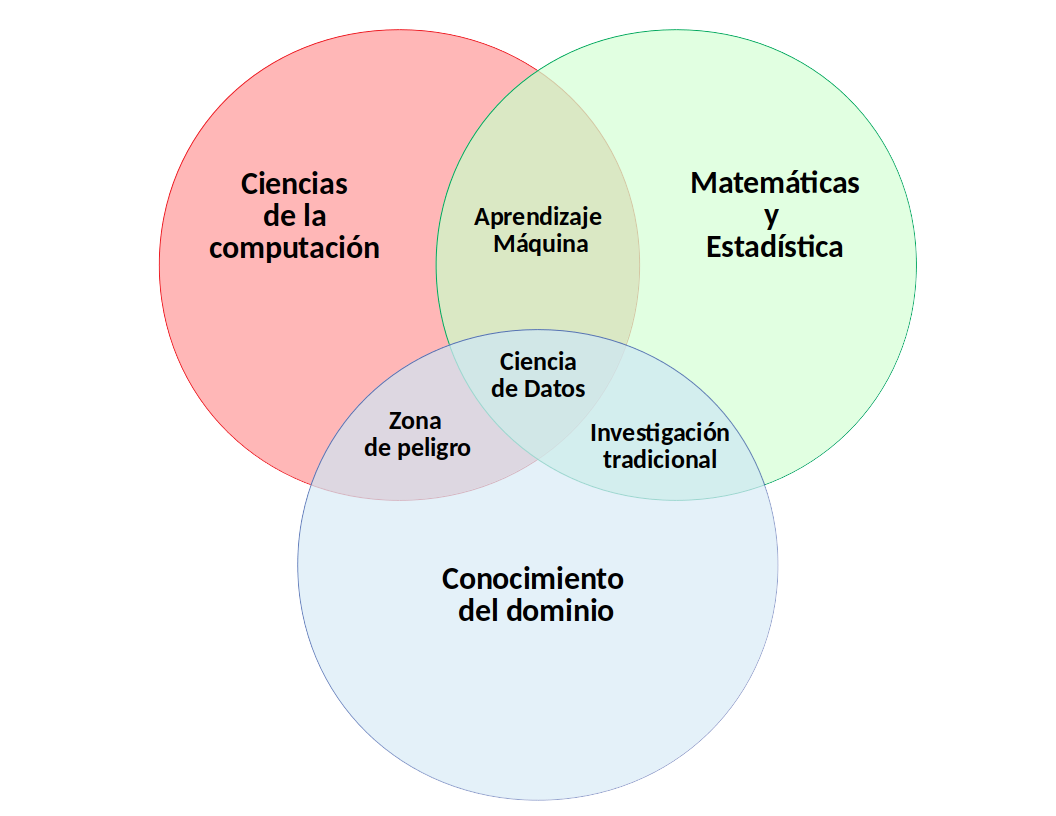
\includegraphics{datascience1.png}

}

\subcaption{\label{fig-ds1}Fundamentos}
\end{minipage}%
%
\begin{minipage}[b]{0.50\linewidth}

{\centering 

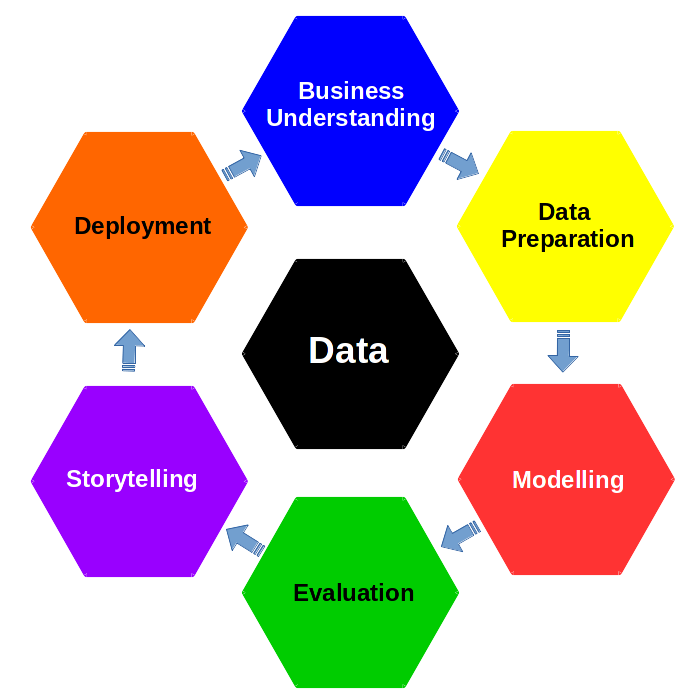
\includegraphics[width=2.86458in,height=\textheight]{datascience_english.png}

}

\subcaption{\label{fig-ds2}Aplicaciones}
\end{minipage}%

\caption{\label{fig-ds}Ciencia de datos}

\end{figure}

La Figura Figure~\ref{fig-ds2} basada en CRISP-DM: ``\emph{Cross
Industry Standard Process for Data Mining}'' (Wirth and Hipp 2000)
presenta el ciclo de vida que todo proyecto de ciencia de datos debería
seguir. El inicio del proyecto viene dado por la definición de los
objetivos de la organización. A continuación, se recogen y gestionan los
datos. Como siguiente paso, se desarrollan y evalúan algoritmos
matemáticos sobre los datos. Los resultados de estos modelos se
presentan a los expertos en el dominio de aplicación para su posterior
integración dentro de la organización. Nótese que el proyecto puede
tener varias iteraciones, volviendo a alguna de las etapas anteriores
siempre que una etapa posterior así lo requiera. Para saber más detalles
sobre estas etapas investigad los paneles siguientes:

\begin{tcolorbox}[enhanced jigsaw, arc=.35mm, breakable, coltitle=black, left=2mm, opacityback=0, bottomtitle=1mm, colbacktitle=quarto-callout-note-color!10!white, title=\textcolor{quarto-callout-note-color}{\faInfo}\hspace{0.5em}{Definir objetivos}, titlerule=0mm, colback=white, colframe=quarto-callout-note-color-frame, bottomrule=.15mm, rightrule=.15mm, opacitybacktitle=0.6, toptitle=1mm, toprule=.15mm, leftrule=.75mm]

Entender el negocio es el primer paso en el proceso. Con ayuda de
expertos en el dominio, se definen las preguntas a responder con el
proyecto (definición de objetivos de la entidad responsable del
proyecto). Una vez comprendido el negocio se designa una solución
analítica para abordar el problema. En esta etapa las reuniones entre
los matemáticos, informáticos y los expertos del dominio (habitualmente
trabajadores con grandes conocimiento del problema que se trata de
abordar) son frecuentes, necesarias y (casi) nunca, suficientes.

\end{tcolorbox}

\begin{tcolorbox}[enhanced jigsaw, arc=.35mm, breakable, coltitle=black, left=2mm, opacityback=0, bottomtitle=1mm, colbacktitle=quarto-callout-note-color!10!white, title=\textcolor{quarto-callout-note-color}{\faInfo}\hspace{0.5em}{Obtener, preparar y gestionar los datos}, titlerule=0mm, colback=white, colframe=quarto-callout-note-color-frame, bottomrule=.15mm, rightrule=.15mm, opacitybacktitle=0.6, toptitle=1mm, toprule=.15mm, leftrule=.75mm]

Mediante técnicas informáticas, se recopilan y se preparan los datos
para su posterior análisis. Podremos hablar de Big Data si los datos se
caracterizan por su \textbf{volumen, variedad o velocidad} de
procesamiento. Todo proceso de Ciencia de Datos es un proceso de
aprendizaje en torno al dato. Las preguntas no surgen de los datos, pero
se necesitan datos para responderlas. Es esta la etapa en la que
trataremos una parte fundamental de todo el proceso: el análisis
exploratorio de datos. Podrás estudiar más sobre cómo preparar los datos
para etapas posteriores en el tema 3 de este libro.

\end{tcolorbox}

\begin{tcolorbox}[enhanced jigsaw, arc=.35mm, breakable, coltitle=black, left=2mm, opacityback=0, bottomtitle=1mm, colbacktitle=quarto-callout-note-color!10!white, title=\textcolor{quarto-callout-note-color}{\faInfo}\hspace{0.5em}{Construir un modelo}, titlerule=0mm, colback=white, colframe=quarto-callout-note-color-frame, bottomrule=.15mm, rightrule=.15mm, opacitybacktitle=0.6, toptitle=1mm, toprule=.15mm, leftrule=.75mm]

A través de métodos matemáticos y estadísticos se estudian y analizan
los datos, se construyen algoritmos y se aplican modelos. Es la etapa
asociada a los modelos de ML que trataremos en los temas 5,7 y 8.

\end{tcolorbox}

\begin{tcolorbox}[enhanced jigsaw, arc=.35mm, breakable, coltitle=black, left=2mm, opacityback=0, bottomtitle=1mm, colbacktitle=quarto-callout-note-color!10!white, title=\textcolor{quarto-callout-note-color}{\faInfo}\hspace{0.5em}{Evaluar y criticar el modelo}, titlerule=0mm, colback=white, colframe=quarto-callout-note-color-frame, bottomrule=.15mm, rightrule=.15mm, opacitybacktitle=0.6, toptitle=1mm, toprule=.15mm, leftrule=.75mm]

Se definen medidas de rendimiento de los modelos que permitan su
evaluación tanto por parte del desarrollador como por parte del cliente.
Trataremos estas medidas en el tema 6 de nuestro curso.

\end{tcolorbox}

\begin{tcolorbox}[enhanced jigsaw, arc=.35mm, breakable, coltitle=black, left=2mm, opacityback=0, bottomtitle=1mm, colbacktitle=quarto-callout-note-color!10!white, title=\textcolor{quarto-callout-note-color}{\faInfo}\hspace{0.5em}{Visualización y presentación}, titlerule=0mm, colback=white, colframe=quarto-callout-note-color-frame, bottomrule=.15mm, rightrule=.15mm, opacitybacktitle=0.6, toptitle=1mm, toprule=.15mm, leftrule=.75mm]

Se presentan los resultados buscando la comprensión por parte del
cliente. No se trata únicamente de aplicar modelos complejos que nadie,
más allá del desarrollador o experto matemático, pueda comprender. Muy
al contrario, existe en la actualidad una corriente de investigación
orientada a construir métodos capaces de ser explicables, junto con
otras técnicas para convertir en entendibles los resultados obtenidos
por los más complejos algoritmos matemáticos. Hablaremos de
explicabilidad de modelos en el último tema del curso.

\end{tcolorbox}

\begin{tcolorbox}[enhanced jigsaw, arc=.35mm, breakable, coltitle=black, left=2mm, opacityback=0, bottomtitle=1mm, colbacktitle=quarto-callout-note-color!10!white, title=\textcolor{quarto-callout-note-color}{\faInfo}\hspace{0.5em}{Despliegue en producción}, titlerule=0mm, colback=white, colframe=quarto-callout-note-color-frame, bottomrule=.15mm, rightrule=.15mm, opacitybacktitle=0.6, toptitle=1mm, toprule=.15mm, leftrule=.75mm]

La solución final se convierte en un producto que podrá ser
comercializado. Los modelos de ML se construyen para un propósito dentro
de una organización. La integración de este modelo dentro del proceso de
la organización debería de ser el último paso del proyecto de ciencia de
datos.

\end{tcolorbox}

En este libro vamos a tratar en profundidad la \emph{Inferencia
Estadística}. Pero, ¿qué relación tiene con la Estadística. Vamos a
verlo.

La estadística es la ciencia que se encarga de recolectar, organizar,
analizar e interpretar datos para tomar decisiones informadas. Su
objetivo principal es comprender y describir la \emph{variabilidad}
inherente en los datos y utilizar esta comprensión para hacer
predicciones y tomar decisiones bajo condiciones de incertidumbre. La
estadística se divide en dos ramas principales:

\begin{tcolorbox}[enhanced jigsaw, arc=.35mm, breakable, coltitle=black, left=2mm, opacityback=0, bottomtitle=1mm, colbacktitle=quarto-callout-note-color!10!white, title=\textcolor{quarto-callout-note-color}{\faInfo}\hspace{0.5em}{Estadística Descriptiva}, titlerule=0mm, colback=white, colframe=quarto-callout-note-color-frame, bottomrule=.15mm, rightrule=.15mm, opacitybacktitle=0.6, toptitle=1mm, toprule=.15mm, leftrule=.75mm]

Se ocupa de resumir y describir las características de un conjunto de
datos mediante herramientas gráficas y numéricas, como tablas, gráficos,
medias, medianas, varianzas, etc. Su objetivo es proporcionar una visión
clara y comprensible de la estructura y características de los datos.

\end{tcolorbox}

\begin{tcolorbox}[enhanced jigsaw, arc=.35mm, breakable, coltitle=black, left=2mm, opacityback=0, bottomtitle=1mm, colbacktitle=quarto-callout-note-color!10!white, title=\textcolor{quarto-callout-note-color}{\faInfo}\hspace{0.5em}{Estadística Inferencial}, titlerule=0mm, colback=white, colframe=quarto-callout-note-color-frame, bottomrule=.15mm, rightrule=.15mm, opacitybacktitle=0.6, toptitle=1mm, toprule=.15mm, leftrule=.75mm]

Utiliza muestras de datos para hacer generalizaciones o inferencias
sobre una población más amplia. Involucra el uso de métodos como la
estimación de parámetros, pruebas de hipótesis y la construcción de
intervalos de confianza. La inferencia estadística permite tomar
decisiones y hacer predicciones basadas en datos muestreados.

\end{tcolorbox}

\hypertarget{sec-inferencia}{%
\section{Inferencia Estadística}\label{sec-inferencia}}

La inferencia estadística se refiere a los métodos y procesos utilizados
para extraer conclusiones acerca de una población a partir de una
muestra de datos. A diferencia de la mera descripción de datos, la
inferencia permite ir más allá de lo observado y hacer generalizaciones,
estimaciones y decisiones en presencia de incertidumbre. Esto es
fundamental para cualquier análisis de datos que aspire a ser predictivo
o que busque comprender fenómenos más amplios que los capturados por los
datos disponibles.

Algunos ejemplos del uso de la inteferencia estadística son:

\begin{itemize}
\tightlist
\item
  Proporción de votantes a un determinado partido,
\item
  Proporción de elementos defectuosos en una partida de productos
\item
  Proporción de paquetes que llegan tarde
\item
  Salario medio
\item
  Altura media
\item
  Concentración media de un componente
\item
  Duración media de un viaje en tren
\item
  Espera media entre dos trenes consecutivos
\end{itemize}

En el contexto de la Ciencia de Datos, la inferencia estadística permite
abordar preguntas críticas como: ¿Cuál es la efectividad de un nuevo
medicamento? ¿Qué factores influyen en la satisfacción del cliente?
¿Cómo se puede predecir el comportamiento futuro de los mercados
financieros? Estas preguntas no solo requieren una recopilación
cuidadosa de datos, sino también un análisis riguroso que tenga en
cuenta la variabilidad inherente y las posibles fuentes de error.

La relevancia de la inferencia estadística en la Ciencia de Datos se
manifiesta en varias áreas clave. Despliega el panel para averiguarlas

\begin{tcolorbox}[enhanced jigsaw, arc=.35mm, breakable, coltitle=black, left=2mm, opacityback=0, bottomtitle=1mm, colbacktitle=quarto-callout-note-color!10!white, title=\textcolor{quarto-callout-note-color}{\faInfo}\hspace{0.5em}{Áreas clave}, titlerule=0mm, colback=white, colframe=quarto-callout-note-color-frame, bottomrule=.15mm, rightrule=.15mm, opacitybacktitle=0.6, toptitle=1mm, toprule=.15mm, leftrule=.75mm]

Estas son algunas de las áreas clave donde la inferencia estadística
cobra valor.

\begin{enumerate}
\def\labelenumi{\arabic{enumi}.}
\item
  \textbf{Modelado Predictivo}: La inferencia estadística es fundamental
  para construir modelos que pueden predecir resultados futuros
  basándose en datos históricos. Estos modelos se utilizan en una
  variedad de campos, desde el marketing hasta la medicina y las
  finanzas.
\item
  \textbf{Análisis Experimental}: En muchos dominios, como la
  biomedicina y la psicología, los experimentos controlados son
  esenciales para determinar causación y no solo correlación. La
  inferencia estadística proporciona el marco para diseñar estos
  experimentos y analizar los resultados de manera adecuada.
\item
  \textbf{Decisiones Basadas en Datos}: En el ámbito empresarial y
  gubernamental, las decisiones basadas en datos permiten optimizar
  procesos, asignar recursos de manera eficiente y mejorar los
  servicios. La inferencia estadística permite que estas decisiones sean
  informadas y respaldadas por evidencia cuantitativa.
\item
  \textbf{Manejo de la Incertidumbre}: En cualquier análisis de datos,
  es crucial manejar y comunicar la incertidumbre. La inferencia
  estadística ofrece métodos para cuantificar esta incertidumbre y tomar
  decisiones informadas pese a la presencia de variabilidad y error.
\end{enumerate}

\end{tcolorbox}

Este libro está diseñado para equipar a los estudiantes del Grado en
Ciencia e Ingeniería de datos con los conocimientos y habilidades
necesarias para aplicar la inferencia estadística en sus estudios y
futuras carreras profesionales. A lo largo de sus capítulos,
exploraremos los fundamentos teóricos y las aplicaciones prácticas de
los métodos inferenciales, proporcionando ejemplos concretos y
ejercicios que reflejan desafíos del mundo real.

La ciencia de datos es un campo dinámico y en constante evolución. La
capacidad de aplicar técnicas de inferencia estadística de manera
efectiva permitirá a los profesionales no solo seguir el ritmo de estos
cambios, sino también liderar innovaciones y descubrimientos basados en
datos. Es nuestra esperanza que este libro sirva como una guía completa
y accesible en este viaje de aprendizaje y aplicación.

Bienvenidos a la apasionante aventura de la inferencia estadística en la
Ciencia de Datos.

\hypertarget{datos-y-variables}{%
\section{Datos y variables}\label{datos-y-variables}}

Los datos son las observaciones o medidas que recopilamos del mundo que
nos rodea. Estos pueden ser números, categorías o cualquier tipo de
información cuantificable. Llamaremos elementos a los individuos, los
sujetos, las observaciones sobre las que se recojen un conjunto de
variables.

\hypertarget{sec-datos}{%
\subsection{Datos en R}\label{sec-datos}}

R incluye en sus librerías numerosos conjuntos de datos. Para acceder a
ellos, basta con cargar la librería correspondiente.

\begin{Shaded}
\begin{Highlighting}[]
\FunctionTok{library}\NormalTok{(tidyverse)}
\FunctionTok{library}\NormalTok{(palmerpenguins)}

\FunctionTok{summary}\NormalTok{(penguins)}
\end{Highlighting}
\end{Shaded}

\begin{verbatim}
      species          island    bill_length_mm  bill_depth_mm  
 Adelie   :152   Biscoe   :168   Min.   :32.10   Min.   :13.10  
 Chinstrap: 68   Dream    :124   1st Qu.:39.23   1st Qu.:15.60  
 Gentoo   :124   Torgersen: 52   Median :44.45   Median :17.30  
                                 Mean   :43.92   Mean   :17.15  
                                 3rd Qu.:48.50   3rd Qu.:18.70  
                                 Max.   :59.60   Max.   :21.50  
                                 NA's   :2       NA's   :2      
 flipper_length_mm  body_mass_g       sex           year     
 Min.   :172.0     Min.   :2700   female:165   Min.   :2007  
 1st Qu.:190.0     1st Qu.:3550   male  :168   1st Qu.:2007  
 Median :197.0     Median :4050   NA's  : 11   Median :2008  
 Mean   :200.9     Mean   :4202                Mean   :2008  
 3rd Qu.:213.0     3rd Qu.:4750                3rd Qu.:2009  
 Max.   :231.0     Max.   :6300                Max.   :2009  
 NA's   :2         NA's   :2                                 
\end{verbatim}

Es posible leer datos desde una cuenta de git. Y podemos tener una
primera visión de los datos con sentencias como\texttt{head} que nos
enseña las primeras observaciones y sus variables.

\begin{Shaded}
\begin{Highlighting}[]
\FunctionTok{library}\NormalTok{ (readr)}

\NormalTok{urlfile}\OtherTok{=}\StringTok{"https://raw.githubusercontent.com/IsaacMartindeDiego/IA/master/datasets/california\_housing.csv"}

\NormalTok{mydata}\OtherTok{\textless{}{-}}\FunctionTok{read\_csv}\NormalTok{(}\FunctionTok{url}\NormalTok{(urlfile))}

\FunctionTok{head}\NormalTok{(mydata)}
\end{Highlighting}
\end{Shaded}

\begin{verbatim}
# A tibble: 6 x 10
  longitude latitude housing_median_age total_rooms total_bedrooms population
      <dbl>    <dbl>              <dbl>       <dbl>          <dbl>      <dbl>
1     -122.     37.9                 41         880            129        322
2     -122.     37.9                 21        7099           1106       2401
3     -122.     37.8                 52        1467            190        496
4     -122.     37.8                 52        1274            235        558
5     -122.     37.8                 52        1627            280        565
6     -122.     37.8                 52         919            213        413
# i 4 more variables: households <dbl>, median_income <dbl>,
#   median_house_value <dbl>, ocean_proximity <chr>
\end{verbatim}

\begin{Shaded}
\begin{Highlighting}[]
\FunctionTok{dim}\NormalTok{(mydata)}
\end{Highlighting}
\end{Shaded}

\begin{verbatim}
[1] 20640    10
\end{verbatim}

\begin{Shaded}
\begin{Highlighting}[]
\FunctionTok{summary}\NormalTok{(mydata)}
\end{Highlighting}
\end{Shaded}

\begin{verbatim}
   longitude         latitude     housing_median_age  total_rooms   
 Min.   :-124.3   Min.   :32.54   Min.   : 1.00      Min.   :    2  
 1st Qu.:-121.8   1st Qu.:33.93   1st Qu.:18.00      1st Qu.: 1448  
 Median :-118.5   Median :34.26   Median :29.00      Median : 2127  
 Mean   :-119.6   Mean   :35.63   Mean   :28.64      Mean   : 2636  
 3rd Qu.:-118.0   3rd Qu.:37.71   3rd Qu.:37.00      3rd Qu.: 3148  
 Max.   :-114.3   Max.   :41.95   Max.   :52.00      Max.   :39320  
                                                                    
 total_bedrooms     population      households     median_income    
 Min.   :   1.0   Min.   :    3   Min.   :   1.0   Min.   : 0.4999  
 1st Qu.: 296.0   1st Qu.:  787   1st Qu.: 280.0   1st Qu.: 2.5634  
 Median : 435.0   Median : 1166   Median : 409.0   Median : 3.5348  
 Mean   : 537.9   Mean   : 1425   Mean   : 499.5   Mean   : 3.8707  
 3rd Qu.: 647.0   3rd Qu.: 1725   3rd Qu.: 605.0   3rd Qu.: 4.7432  
 Max.   :6445.0   Max.   :35682   Max.   :6082.0   Max.   :15.0001  
 NA's   :207                                                        
 median_house_value ocean_proximity   
 Min.   : 14999     Length:20640      
 1st Qu.:119600     Class :character  
 Median :179700     Mode  :character  
 Mean   :206856                       
 3rd Qu.:264725                       
 Max.   :500001                       
                                      
\end{verbatim}

La estructura de datos más habitual para realizar análisis de datos es
el \texttt{data\ frame}. ¿Has estudiado este concepto en cursos
anteriores?. Los \texttt{data\ frame} son estructuras de datos de dos
dimensiones (como una matriz) que pueden contener datos de diferentes
tipos. Normalmente nos referimos a las filas de un data frame como
observaciones o registros, mientras que las columnas reciben el nombre
de campos, variables, o características.

\begin{Shaded}
\begin{Highlighting}[]
\NormalTok{L3 }\OtherTok{\textless{}{-}}\NormalTok{ LETTERS[}\DecValTok{1}\SpecialCharTok{:}\DecValTok{3}\NormalTok{]}
\NormalTok{char }\OtherTok{\textless{}{-}} \FunctionTok{sample}\NormalTok{(L3, }\DecValTok{10}\NormalTok{, }\AttributeTok{replace =} \ConstantTok{TRUE}\NormalTok{)}
\NormalTok{datos }\OtherTok{\textless{}{-}} \FunctionTok{data.frame}\NormalTok{(}\AttributeTok{x =} \DecValTok{1}\NormalTok{, }\AttributeTok{y =} \DecValTok{1}\SpecialCharTok{:}\DecValTok{10}\NormalTok{, }\AttributeTok{char =}\NormalTok{ char)}
\NormalTok{datos}
\end{Highlighting}
\end{Shaded}

\begin{verbatim}
   x  y char
1  1  1    B
2  1  2    C
3  1  3    B
4  1  4    C
5  1  5    C
6  1  6    A
7  1  7    C
8  1  8    C
9  1  9    B
10 1 10    C
\end{verbatim}

\begin{Shaded}
\begin{Highlighting}[]
\FunctionTok{is.data.frame}\NormalTok{(datos)}
\end{Highlighting}
\end{Shaded}

\begin{verbatim}
[1] TRUE
\end{verbatim}

Un \textbf{tibble}, o tbl\_df, es una actualización del concepto del
data frame. Los tibbles son data.frames perezosos. Esto le obliga a
enfrentarse a los problemas antes, lo que normalmente conduce a un
código más limpio y expresivo. Los tibbles también tienen un método
\texttt{print()} mejorado que facilita su uso con grandes conjuntos de
datos que contienen objetos complejos.

\begin{Shaded}
\begin{Highlighting}[]
\FunctionTok{library}\NormalTok{(tidyverse)}
\FunctionTok{as.tibble}\NormalTok{(iris)}
\end{Highlighting}
\end{Shaded}

\begin{verbatim}
# A tibble: 150 x 5
   Sepal.Length Sepal.Width Petal.Length Petal.Width Species
          <dbl>       <dbl>        <dbl>       <dbl> <fct>  
 1          5.1         3.5          1.4         0.2 setosa 
 2          4.9         3            1.4         0.2 setosa 
 3          4.7         3.2          1.3         0.2 setosa 
 4          4.6         3.1          1.5         0.2 setosa 
 5          5           3.6          1.4         0.2 setosa 
 6          5.4         3.9          1.7         0.4 setosa 
 7          4.6         3.4          1.4         0.3 setosa 
 8          5           3.4          1.5         0.2 setosa 
 9          4.4         2.9          1.4         0.2 setosa 
10          4.9         3.1          1.5         0.1 setosa 
# i 140 more rows
\end{verbatim}

\begin{tcolorbox}[enhanced jigsaw, arc=.35mm, breakable, coltitle=black, left=2mm, opacityback=0, bottomtitle=1mm, colbacktitle=quarto-callout-caution-color!10!white, title=\textcolor{quarto-callout-caution-color}{\faFire}\hspace{0.5em}{Práctica}, titlerule=0mm, colback=white, colframe=quarto-callout-caution-color-frame, bottomrule=.15mm, rightrule=.15mm, opacitybacktitle=0.6, toptitle=1mm, toprule=.15mm, leftrule=.75mm]

Es importante que realices algún ejercicio en R, leyendo datos de
diferentes fuentes y familiarizándote con las diferentes estructuras de
datos que R proporciona.

\end{tcolorbox}

\hypertarget{tipo-de-variables}{%
\subsection{Tipo de variables}\label{tipo-de-variables}}

Una \textbf{variable} es una característica o atributo que se pueden
observar en los elementos y que puede tomar diferentes valores.
Llamaremos valores a los resultados que se pueden observar de la
característica en el elemento. Las variables siguen una distribución de
probabilidad. Las variables pueden ser de varios tipos:

\begin{itemize}
\item
  Cualitativas: También conocidas como categóricas, estas variables
  describen atributos o cualidades y se dividen en nominales (sin orden
  específico, como colores) y ordinales (con un orden, como niveles de
  satisfacción).
\item
  Cuantitativas: Estas variables son numéricas y pueden ser discretas
  (valores contables, como el número de hijos) o continuas (valores
  dentro de un rango, como la altura o el peso).
\item
  Marcas de tiempo o identificadores: Como por ejemplo la fecha y hora
  de una transacción o el código de un producto o el número de
  identidad.
\end{itemize}

En este tema vamos a trabajar con los datos de
\href{https://archive.ics.uci.edu/dataset/222/bank+marketing}{\textbf{Bank
Marketing}} del repositorio UCI. En primer lugar debemos comprender el
problema. ¿Qué sabes del marketing bancario? En el caso que nos ocupa,
los datos están relacionados con campañas de marketing directo (llamadas
telefónicas) de una entidad bancaria portuguesa. El objetivo de la
clasificación es \emph{predecir si el cliente suscribirá un depósito} a
plazo (variable objetivo).

Las variables que debemos estudiar son:

Variables de entrada:

\# datos del cliente bancario:

\begin{enumerate}
\def\labelenumi{\arabic{enumi}.}
\item
  edad (variable numérica)
\item
  empleo : tipo de empleo (variable categórica con las siguientes
  categorías: ``admin.'', ``desconocido'', ``desempleado'',
  ``directivo'', ``empleada del hogar'', ``empresario'', ``estudiante'',
  ``obrero'', ``autónomo'', ``jubilado'', ``técnico'', ``servicios'')
\item
  estado civil : estado civil (variable categórica con categorías:
  ``casado'', ``divorciado'', ``soltero''; nota: ``divorciado''
  significa divorciado o viudo)
\item
  educación (variable categórica con categorías: ``desconocida'',
  ``secundaria'', ``primaria'', ``terciaria'')
\item
  impago: ¿tiene un crédito impagado? (variable binaria con dos posibles
  valores: ``sí'', ``no'')
\item
  saldo: saldo medio anual, en euros (variable numérica)
\item
  vivienda: ¿tiene préstamo para vivienda? (variable binaria: ``sí'',
  ``no'')
\item
  préstamo: ¿tiene préstamo personal? (variable binaria: ``sí'', ``no'')

  \# relacionado con el último contacto de la campaña actual:
\item
  contacto: tipo de comunicación del contacto (variable categórica:
  ``desconocido'', ``teléfono'', ``móvil'')
\item
  día: día del mes del último contacto (variable numérica)
\item
  mes: mes del año del último contacto (variable categórica: ``ene'',
  ``feb'', ``mar'', \ldots, ``nov'', ``dic'')
\item
  duración: duración del último contacto, en segundos (variable
  numérica)
\end{enumerate}

\# otros atributos

\begin{enumerate}
\def\labelenumi{\arabic{enumi}.}
\setcounter{enumi}{12}
\item
  campaña: número de contactos realizados durante esta campaña y para
  este cliente (variable numérica, incluye el último contacto)
\item
  pdays: número de días transcurridos desde que el cliente fue
  contactado por última vez en una campaña anterior (variable numérica,
  -1 significa que el cliente no fue contactado previamente)
\item
  previous: número de contactos realizados antes de esta campaña y para
  este cliente (variable numérica)
\item
  poutcome: resultado de la campaña de marketing anterior (variable
  categórica: ``desconocido'', ``otro'', ``fracaso'', ``éxito'')
\end{enumerate}

\# Variable de salida (objetivo deseado):

17 - y: ¿ha suscrito el cliente un depósito a plazo? (variable binaria:
``sí'', ``no'')

\begin{tcolorbox}[enhanced jigsaw, arc=.35mm, breakable, coltitle=black, left=2mm, opacityback=0, bottomtitle=1mm, colbacktitle=quarto-callout-important-color!10!white, title=\textcolor{quarto-callout-important-color}{\faExclamation}\hspace{0.5em}{Para recordar}, titlerule=0mm, colback=white, colframe=quarto-callout-important-color-frame, bottomrule=.15mm, rightrule=.15mm, opacitybacktitle=0.6, toptitle=1mm, toprule=.15mm, leftrule=.75mm]

A veces (muchas veces) la descripción que encontramos en una primera
etapa no coincide al completo con los datos que luego nos entrega el
cliente.

En otras ocasiones no se dispone de la descripción de las variables. En
ese caso, ¡hay que hacer lo imposible por conseguirla!

\end{tcolorbox}

Leemos los datos con R.

\begin{Shaded}
\begin{Highlighting}[]
\FunctionTok{library}\NormalTok{(tidyverse)}
\NormalTok{bank }\OtherTok{=} \FunctionTok{read.csv}\NormalTok{(}\StringTok{\textquotesingle{}https://raw.githubusercontent.com/rafiag/DTI2020/main/data/bank.csv\textquotesingle{}}\NormalTok{)}
\FunctionTok{dim}\NormalTok{(bank)}
\end{Highlighting}
\end{Shaded}

\begin{verbatim}
[1] 11162    17
\end{verbatim}

\begin{Shaded}
\begin{Highlighting}[]
\NormalTok{bank}\OtherTok{=}\FunctionTok{as.tibble}\NormalTok{(bank)}
\NormalTok{bank}
\end{Highlighting}
\end{Shaded}

\begin{verbatim}
# A tibble: 11,162 x 17
     age job       marital education default balance housing loan  contact   day
   <int> <chr>     <chr>   <chr>     <chr>     <int> <chr>   <chr> <chr>   <int>
 1    59 admin.    married secondary no         2343 yes     no    unknown     5
 2    56 admin.    married secondary no           45 no      no    unknown     5
 3    41 technici~ married secondary no         1270 yes     no    unknown     5
 4    55 services  married secondary no         2476 yes     no    unknown     5
 5    54 admin.    married tertiary  no          184 no      no    unknown     5
 6    42 manageme~ single  tertiary  no            0 yes     yes   unknown     5
 7    56 manageme~ married tertiary  no          830 yes     yes   unknown     6
 8    60 retired   divorc~ secondary no          545 yes     no    unknown     6
 9    37 technici~ married secondary no            1 yes     no    unknown     6
10    28 services  single  secondary no         5090 yes     no    unknown     6
# i 11,152 more rows
# i 7 more variables: month <chr>, duration <int>, campaign <int>, pdays <int>,
#   previous <int>, poutcome <chr>, deposit <chr>
\end{verbatim}

Disponemos de más de 10000 observaciones y un total de 17 variables.

Para averiguar qué tipo de variables manejamos, ejecutar:

\begin{Shaded}
\begin{Highlighting}[]
\FunctionTok{str}\NormalTok{(bank)}
\end{Highlighting}
\end{Shaded}

\begin{verbatim}
tibble [11,162 x 17] (S3: tbl_df/tbl/data.frame)
 $ age      : int [1:11162] 59 56 41 55 54 42 56 60 37 28 ...
 $ job      : chr [1:11162] "admin." "admin." "technician" "services" ...
 $ marital  : chr [1:11162] "married" "married" "married" "married" ...
 $ education: chr [1:11162] "secondary" "secondary" "secondary" "secondary" ...
 $ default  : chr [1:11162] "no" "no" "no" "no" ...
 $ balance  : int [1:11162] 2343 45 1270 2476 184 0 830 545 1 5090 ...
 $ housing  : chr [1:11162] "yes" "no" "yes" "yes" ...
 $ loan     : chr [1:11162] "no" "no" "no" "no" ...
 $ contact  : chr [1:11162] "unknown" "unknown" "unknown" "unknown" ...
 $ day      : int [1:11162] 5 5 5 5 5 5 6 6 6 6 ...
 $ month    : chr [1:11162] "may" "may" "may" "may" ...
 $ duration : int [1:11162] 1042 1467 1389 579 673 562 1201 1030 608 1297 ...
 $ campaign : int [1:11162] 1 1 1 1 2 2 1 1 1 3 ...
 $ pdays    : int [1:11162] -1 -1 -1 -1 -1 -1 -1 -1 -1 -1 ...
 $ previous : int [1:11162] 0 0 0 0 0 0 0 0 0 0 ...
 $ poutcome : chr [1:11162] "unknown" "unknown" "unknown" "unknown" ...
 $ deposit  : chr [1:11162] "yes" "yes" "yes" "yes" ...
\end{verbatim}

\begin{tcolorbox}[enhanced jigsaw, arc=.35mm, breakable, coltitle=black, left=2mm, opacityback=0, bottomtitle=1mm, colbacktitle=quarto-callout-caution-color!10!white, title=\textcolor{quarto-callout-caution-color}{\faFire}\hspace{0.5em}{Ejercicio}, titlerule=0mm, colback=white, colframe=quarto-callout-caution-color-frame, bottomrule=.15mm, rightrule=.15mm, opacitybacktitle=0.6, toptitle=1mm, toprule=.15mm, leftrule=.75mm]

Identifica el tipo de cada variable y las unidades de medida.

\end{tcolorbox}

\hypertarget{escalas-de-mediciuxf3n}{%
\subsection{Escalas de medición}\label{escalas-de-mediciuxf3n}}

Una escala de medición define cómo se cuantifican o categorizan las
variables recogidas sobre un conjunto de datos, influyendo en el
análisis estadístico aplicable.

\begin{itemize}
\item
  \textbf{Nominal}: categorización sin orden inherente. Por ejemplo, el
  género, la nacionalidad o el tipo de sangre.
\item
  \textbf{Ordinal}: categorización con un orden lógico. Por ejemplo, el
  nivel educativo, o una clasificación de hoteles.
\item
  \textbf{Métrica}: medición de diferentes escalas:

  \begin{itemize}
  \item
    Intervalo: sin cero verdadero, por ejemplo la temperatura en
    Celsius.
  \item
    Razón: con cero verdadero, por ejemplo los ingresos o la distancia.
  \end{itemize}
\end{itemize}

En estadística y análisis de datos, es muy común recurrir a conversión
entre diferentes escalas de medición. Las más comunes son:

\begin{itemize}
\tightlist
\item
  Fechas a categóricas: convertir fechas exactas en mes, día de la
  semana, etc.
\item
  Cuantitativas a cualitativas: crear clases o rangos a partir de datos
  numéricos. Por ejemplo convertir el nivel de ingresos en ``bajo'',
  ``medio'' y ``alto''.
\item
  Ordinales como numéricas: pasar de un orden a unos valores numéricos
  puede ser peligroso. Esta transformación ha de ser empleada con
  precaución, especialmente cuando se trabaja con pocos datos
  (\(<100\)). Ten en cuenta que combinar en índices puede ser más
  informativo.
\item
  Variables calculadas: creación de nuevas variables a partir de las
  existentes es una práctica muy habitual en análisis de datos. Hay una
  gran cantidad de situaciones donde esta tarea será muy beneficiosa.
  Por ejemplo, se crea el Índice de Masa Corporal (IMC) a partir de peso
  y altura.
\end{itemize}

\hypertarget{poblaciuxf3n-y-muestra}{%
\section{Población y muestra}\label{poblaciuxf3n-y-muestra}}

La \textbf{población} es el conjunto completo de todos los elementos o
individuos que se desean estudiar. Puede ser una colección de personas,
objetos, eventos o cualquier unidad de observación que sea de interés en
un estudio. Por ejemplo, la población podría ser todos los estudiantes
de una universidad, todos los árboles en un bosque, o todos los
productos fabricados en una planta.

Dado que es a menudo impráctico o imposible estudiar toda la población,
se selecciona una muestra, que es un subconjunto de la población. El
estudio de las observaciones de una población podría implicar destruir
dichas observaciones (vida útil del componente). El coste del estudio de
las características de las observaciones podría ser muy elevado
(experimentos biológicos). A veces el tamaño de la población es tan
elevado (\emph{very big data!}) que es obligatorio utilizar métodos de
muestreo. Eso sí, es importante que la muestra sea representativa para
que las conclusiones que se extraen de ella sean válidas para la
población completa.

\begin{tcolorbox}[enhanced jigsaw, arc=.35mm, breakable, coltitle=black, left=2mm, opacityback=0, bottomtitle=1mm, colbacktitle=quarto-callout-tip-color!10!white, title=\textcolor{quarto-callout-tip-color}{\faLightbulb}\hspace{0.5em}{Ejemplo. Sondeo Electoral de 1936}, titlerule=0mm, colback=white, colframe=quarto-callout-tip-color-frame, bottomrule=.15mm, rightrule=.15mm, opacitybacktitle=0.6, toptitle=1mm, toprule=.15mm, leftrule=.75mm]

El caso del sondeo electoral de 1936, realizado por la revista
``Literary Digest'' en Estados Unidos, es un ejemplo clásico que ilustra
la importancia de la representatividad de una muestra en la
investigación estadística y en particular en la realización de
encuestas.

En 1936, la revista ``Literary Digest'' llevó a cabo un sondeo para
predecir el resultado de la elección presidencial entre el candidato
demócrata Franklin D. Roosevelt y el candidato republicano Alf Landon.
La revista enviaba millones de encuestas a sus lectores y a otras listas
de individuos, como propietarios de automóviles y personas que aparecían
en directorios telefónicos. En ese año, ``Literary Digest'' envió unos
10 millones de encuestas y recibió alrededor de 2.4 millones de
respuestas, lo que constituía una muestra enorme para los estándares de
la época.

La predicción del sondeo fue que Alf Landon ganaría la elección con un
margen significativo. Sin embargo, el resultado real fue una victoria
aplastante para Franklin D. Roosevelt, quien ganó con más del 60\% del
voto popular y el 98.5\% del voto electoral. Este error de predicción se
debió principalmente a problemas relacionados con la representatividad
de la muestra.

\textbf{Problemas de Representatividad}

\begin{enumerate}
\def\labelenumi{\arabic{enumi}.}
\item
  \textbf{Sesgo de Selección}: La muestra del sondeo no era
  representativa de la población general. La lista de encuestados estaba
  basada en suscriptores de la revista, propietarios de automóviles y
  personas que aparecían en directorios telefónicos. En la década de
  1930, estos grupos eran, en su mayoría, personas de ingresos más altos
  y de tendencia republicana, que no representaban adecuadamente a la
  población estadounidense en general, que incluía una proporción
  significativa de votantes de ingresos más bajos y de tendencia
  demócrata.
\item
  \textbf{Tasa de Respuesta}: Aunque el tamaño de la muestra era grande
  (2.4 millones de respuestas), la tasa de respuesta fue baja en
  relación al número de encuestas enviadas (10 millones). Esto puede
  introducir un sesgo adicional, ya que las personas que respondieron
  pueden no ser representativas de la población objetivo. Es posible que
  aquellos más inclinados a responder fueran también más inclinados a
  votar por Landon.
\item
  \textbf{Muestreo No Aleatorio}: El método de selección de la muestra
  no era aleatorio. Las listas utilizadas para enviar las encuestas no
  cubrían todas las demografías de manera equitativa. Un muestreo
  aleatorio hubiera asegurado que cada individuo de la población tuviera
  una probabilidad conocida y no nula de ser seleccionado, lo cual es
  crucial para la representatividad.
\end{enumerate}

\end{tcolorbox}

La \textbf{probabilidad} juega un papel crucial en el diseño del
muestreo y en la inferencia estadística. En el contexto del muestreo, la
probabilidad asegura que cada miembro de la población tiene una
oportunidad conocida y, generalmente, igual de ser incluido en la
muestra. Esto permite que las muestras sean representativas y que los
resultados sean generalizables. La teoría de la probabilidad también se
utiliza para modelar la incertidumbre y el comportamiento aleatorio
inherente en los datos.

\begin{tcolorbox}[enhanced jigsaw, arc=.35mm, breakable, coltitle=black, left=2mm, opacityback=0, bottomtitle=1mm, colbacktitle=quarto-callout-warning-color!10!white, title=\textcolor{quarto-callout-warning-color}{\faExclamationTriangle}\hspace{0.5em}{Warning}, titlerule=0mm, colback=white, colframe=quarto-callout-warning-color-frame, bottomrule=.15mm, rightrule=.15mm, opacitybacktitle=0.6, toptitle=1mm, toprule=.15mm, leftrule=.75mm]

Probablemente has estudiado estos conceptos en la asignatura de
\emph{Probabilidad y Simulación}.

\end{tcolorbox}

Una vez que se ha recolectado una muestra, la \textbf{estadística
descriptiva} se utiliza para organizar, resumir y presentar los datos de
manera comprensible. Las herramientas de estadística descriptiva
incluyen:

\begin{itemize}
\tightlist
\item
  Medidas de tendencia central: como la media, mediana y moda, que
  resumen el centro de los datos.
\item
  Medidas de dispersión: como el rango, la varianza y la desviación
  estándar, que describen la variabilidad de los datos.
\item
  Gráficos: como histogramas, gráficos de caja y gráficos de dispersión,
  que visualizan los datos.
\end{itemize}

La estadística descriptiva se centra en describir lo que los datos
muestran, sin hacer inferencias o generalizaciones sobre la población.

La \textbf{inferencia estadística} utiliza los datos de la muestra para
hacer estimaciones, predicciones y generalizaciones sobre la población
completa. Esto incluye dos aspectos principales:

\begin{itemize}
\tightlist
\item
  Estimación: Utilizar los datos de la muestra para estimar parámetros
  de la población, como la media o la proporción. Las estimaciones
  pueden ser puntuales (un solo valor) o por intervalo (un rango de
  valores con un nivel de confianza asociado).
\item
  Contraste de hipótesis: Probar afirmaciones sobre la población
  utilizando los datos de la muestra. Esto implica formular una
  hipótesis nula y una hipótesis alternativa, y usar pruebas
  estadísticas para decidir cuál es más consistente con los datos
  observados.
\end{itemize}

La inferencia estadística se basa en la teoría de la probabilidad para
evaluar la incertidumbre y la variabilidad en las estimaciones y
pruebas.

La Figure~\ref{fig-muestreo} muestra la relación entre los conceptos de
Población, Muestra, Inferencia Estadística, Probabilida y Estadística
Descriptiva. Estos conceptos permiten a los estadísticos recolectar
datos de manera eficiente, describir los datos recolectados y hacer
inferencias significativas y precisas sobre la población a partir de la
muestra.

\begin{figure}

{\centering 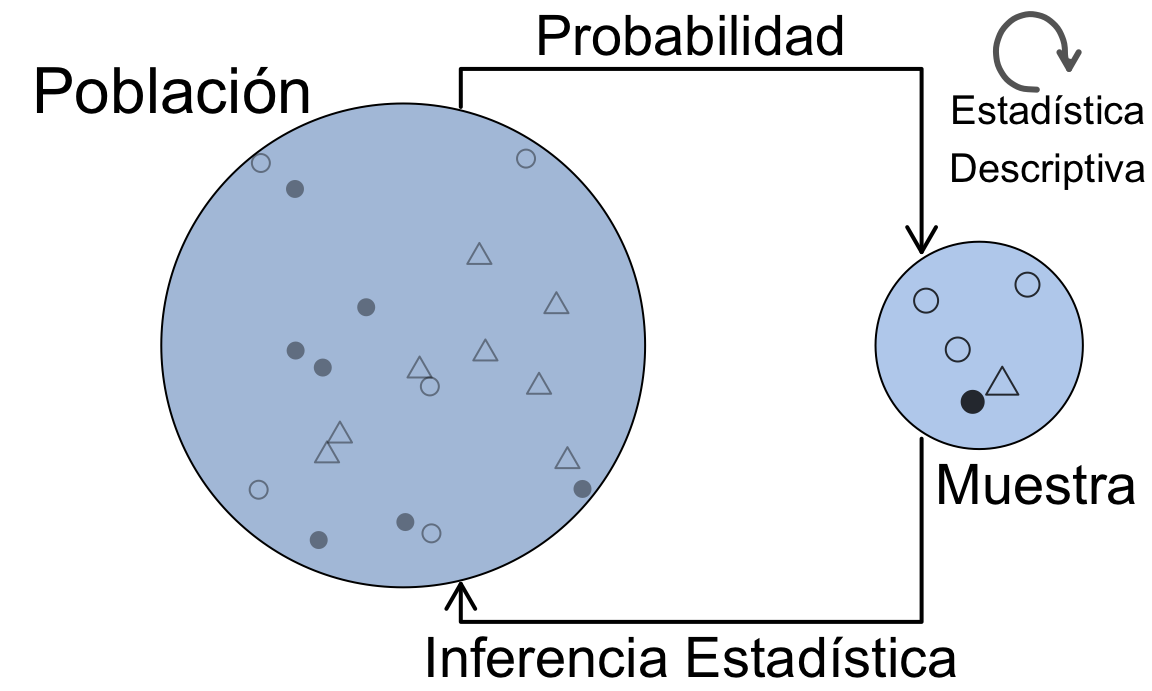
\includegraphics[width=0.5\textwidth,height=\textheight]{dogma1.png}

}

\caption{\label{fig-muestreo}La esencia de la Estadística}

\end{figure}

Existe un principio fundamental en el análisis de datos que podríamos
simplificar así:

\[DATOS = MODELO + ERROR\]

\begin{itemize}
\item
  Los \textbf{datos} representan la realidad (procesos de negocios,
  clientes, productos, actividades, fenómenos físicos, etc.) que se
  quiere comprender, predecir o mejorar.
\item
  El \textbf{modelo} es una representación \textbf{simplificada} de la
  realidad que proponemos para describirla e interpretarla más
  fácilmente.
\item
  El \textbf{error} refleja la diferencia entre nuestra representación
  simplificada de la realidad (el modelo) y los datos que relamente
  describen esa realidad de forma precisa.
\end{itemize}

Buscaremos encontrar el modelo que explique los datos minimizando al
máximo el error.

\hypertarget{muestreo}{%
\subsection{Muestreo}\label{muestreo}}

El muestreo estadístico es una técnica fundamental en la estadística que
permite extraer conclusiones sobre una población basándose en el
análisis de una parte más pequeña de dicha población, conocida como
muestra. A continuación, presentamos algunas de las principales técnicas
de muestreo estadístico. Cada una de estas técnicas tiene sus propias
ventajas y limitaciones, y la elección de la técnica adecuada depende
del objetivo del estudio, las características de la población y los
recursos disponibles.

\hypertarget{muestreo-aleatorio-simple}{%
\subsubsection{Muestreo Aleatorio
Simple}\label{muestreo-aleatorio-simple}}

En el muestreo aleatorio simple, cada miembro de la población tiene la
misma probabilidad de ser seleccionado. Diremos que la muestra es
aletoria simple (\textbf{m.a.s.}) cuando empleamos este tipo de
muestroe. Se suele realizar utilizando métodos aleatorios, como sorteo,
tablas de números aleatorios o generadores de números aleatorios. Este
método es simple y fácil de entender, pero puede no ser siempre el más
eficiente, especialmente si la población es muy grande. Podemos realizar
el muestro con o sin reemplazamiento. Diremos que un muestreo es con
reemplazamiento cuando una observación poblacional puede ser elegida
varias veces para formar parte de la muestra. La misma observación puede
aparecer repetida. Habitualmente se recurre al muestro sin
reemplazamiento, donde una observación población, una vez elegida para
formar parte de la muestra, es eliminada de la población y no puede
volver a ser elegida.

La siguiente sentencia de \texttt{R} elige \(5\) observaciones de la
base de datos \texttt{bank} mediante un muestreo aleatorio simple.

\begin{Shaded}
\begin{Highlighting}[]
\NormalTok{n}\OtherTok{=}\FunctionTok{dim}\NormalTok{(bank)[}\DecValTok{1}\NormalTok{] }\CommentTok{\# número de observaciones en la base de datos}
\NormalTok{indices}\OtherTok{=}\FunctionTok{sample}\NormalTok{(}\DecValTok{1}\SpecialCharTok{:}\NormalTok{n,}\AttributeTok{size=}\DecValTok{5}\NormalTok{,}\AttributeTok{replace=}\ConstantTok{FALSE}\NormalTok{)}
\NormalTok{indices }\CommentTok{\# indices de las observaciones elegidas}
\end{Highlighting}
\end{Shaded}

\begin{verbatim}
[1] 2220 6790  637 8636 7653
\end{verbatim}

\begin{Shaded}
\begin{Highlighting}[]
\NormalTok{muestra}\OtherTok{=}\NormalTok{bank[indices,] }\CommentTok{\# muestra de observaciones }
\end{Highlighting}
\end{Shaded}

Esta técnica será empleada en la asignatura de \textbf{Aprendizaje
Automático} para crear las particiones de entrenamiento, test y
validación.

Para aprender otros tipos de muestreos, despliega los siguientes
paneles:

\begin{tcolorbox}[enhanced jigsaw, arc=.35mm, breakable, coltitle=black, left=2mm, opacityback=0, bottomtitle=1mm, colbacktitle=quarto-callout-note-color!10!white, title=\textcolor{quarto-callout-note-color}{\faInfo}\hspace{0.5em}{Muestreo Sistemático}, titlerule=0mm, colback=white, colframe=quarto-callout-note-color-frame, bottomrule=.15mm, rightrule=.15mm, opacitybacktitle=0.6, toptitle=1mm, toprule=.15mm, leftrule=.75mm]

En el muestreo sistemático, se selecciona un punto de inicio al azar y
luego se elige a cada n-ésimo individuo de la lista de la población. Por
ejemplo, si se quiere una muestra del 10\% de una población de 1000
individuos, se seleccionaría un punto de inicio al azar entre los
primeros 10 individuos y luego se seleccionaría cada décimo individuo a
partir de ese punto. Este método es más fácil de ejecutar que el
muestreo aleatorio simple, pero puede introducir sesgos si hay un patrón
en la lista de la población.

\end{tcolorbox}

\begin{tcolorbox}[enhanced jigsaw, arc=.35mm, breakable, coltitle=black, left=2mm, opacityback=0, bottomtitle=1mm, colbacktitle=quarto-callout-note-color!10!white, title=\textcolor{quarto-callout-note-color}{\faInfo}\hspace{0.5em}{Muestreo Estratificado}, titlerule=0mm, colback=white, colframe=quarto-callout-note-color-frame, bottomrule=.15mm, rightrule=.15mm, opacitybacktitle=0.6, toptitle=1mm, toprule=.15mm, leftrule=.75mm]

El muestreo estratificado implica dividir la población en subgrupos o
estratos homogéneos y luego tomar una muestra aleatoria de cada estrato.
Los estratos se forman en base a una característica específica como la
edad, el género, el nivel socioeconómico, etc. Este método asegura que
todas las subpoblaciones importantes estén representadas en la muestra y
puede proporcionar estimaciones más precisas que el muestreo aleatorio
simple. En el Aprendizaje Automático la variable elegida será la
variable respuesta, o variable objetivo. De este modo, cuando los datos
están desequilibrados, es decir, cuando tenemos más observaciones de una
clase que de otra en los valores de la variable respuesta, aseguramos
que todas los grupos están igualmente representados en la myestra.

\end{tcolorbox}

\begin{tcolorbox}[enhanced jigsaw, arc=.35mm, breakable, coltitle=black, left=2mm, opacityback=0, bottomtitle=1mm, colbacktitle=quarto-callout-note-color!10!white, title=\textcolor{quarto-callout-note-color}{\faInfo}\hspace{0.5em}{Muestreo por Conglomerados}, titlerule=0mm, colback=white, colframe=quarto-callout-note-color-frame, bottomrule=.15mm, rightrule=.15mm, opacitybacktitle=0.6, toptitle=1mm, toprule=.15mm, leftrule=.75mm]

En el muestreo por conglomerados, la población se divide en grupos o
conglomerados, y se seleccionan algunos de estos conglomerados al azar.
Luego, todos los individuos dentro de los conglomerados seleccionados se
incluyen en la muestra. Este método es útil cuando es difícil o costoso
crear una lista completa de la población, pero puede ser menos preciso
si los conglomerados no son homogéneos.

\end{tcolorbox}

\begin{tcolorbox}[enhanced jigsaw, arc=.35mm, breakable, coltitle=black, left=2mm, opacityback=0, bottomtitle=1mm, colbacktitle=quarto-callout-note-color!10!white, title=\textcolor{quarto-callout-note-color}{\faInfo}\hspace{0.5em}{Muestreo por Cuotas}, titlerule=0mm, colback=white, colframe=quarto-callout-note-color-frame, bottomrule=.15mm, rightrule=.15mm, opacitybacktitle=0.6, toptitle=1mm, toprule=.15mm, leftrule=.75mm]

El muestreo por cuotas es un tipo de muestreo no probabilístico en el
que se selecciona una muestra que cumple con ciertas cuotas
preestablecidas basadas en características específicas. Por ejemplo, se
puede querer que la muestra tenga un cierto número de individuos de
diferentes edades o géneros. Aunque este método es práctico y rápido, no
permite estimaciones estadísticas precisas de la población porque no
todos los individuos tienen la misma probabilidad de ser seleccionados.

\end{tcolorbox}

\begin{tcolorbox}[enhanced jigsaw, arc=.35mm, breakable, coltitle=black, left=2mm, opacityback=0, bottomtitle=1mm, colbacktitle=quarto-callout-note-color!10!white, title=\textcolor{quarto-callout-note-color}{\faInfo}\hspace{0.5em}{Muestreo de Bola de Nieve}, titlerule=0mm, colback=white, colframe=quarto-callout-note-color-frame, bottomrule=.15mm, rightrule=.15mm, opacitybacktitle=0.6, toptitle=1mm, toprule=.15mm, leftrule=.75mm]

El muestreo de bola de nieve es otra técnica no probabilística,
utilizada principalmente cuando es difícil acceder a los miembros de la
población. Se empieza con unos pocos individuos conocidos de la
población, quienes a su vez refieren a otros individuos, y así
sucesivamente. Este método es útil para estudios de poblaciones ocultas
o difíciles de alcanzar, como personas sin hogar o usuarios de drogas,
pero introduce un alto riesgo de sesgo. Es muy común utilizar este tipo
de muestreo cuando se realizan encuestas en redes sociales.

\end{tcolorbox}

\begin{tcolorbox}[enhanced jigsaw, arc=.35mm, breakable, coltitle=black, left=2mm, opacityback=0, bottomtitle=1mm, colbacktitle=quarto-callout-note-color!10!white, title=\textcolor{quarto-callout-note-color}{\faInfo}\hspace{0.5em}{Muestreo Intencional o Dirigido}, titlerule=0mm, colback=white, colframe=quarto-callout-note-color-frame, bottomrule=.15mm, rightrule=.15mm, opacitybacktitle=0.6, toptitle=1mm, toprule=.15mm, leftrule=.75mm]

En el muestreo intencional o dirigido, se seleccionan individuos que
cumplen con ciertos criterios específicos de la investigación. Es un
método no probabilístico donde la selección se basa en el juicio del
investigador. Es útil cuando se busca estudiar casos específicos, pero
no permite hacer generalizaciones precisas sobre la población completa.

\end{tcolorbox}

\hypertarget{paruxe1metros-y-estaduxedsticos}{%
\section{Parámetros y
Estadísticos}\label{paruxe1metros-y-estaduxedsticos}}

Los \textbf{parámetros} son (casi) siempre desconocidos. Son valores
teóricos que se definen sobre la población. Son sobre los que haremos
\emph{inferencia}. Normalmente se representan con letras griegas.

Diremos que un \textbf{estadístico} (además de un señor que hace
estadística) es una función definida sobre los datos de una muestra
(valores de una o más variables). En cada muestra serán distintos,
debido a la variabilidad inherente a la extracción de una muestra
representativa de una población. Los estadísticos siguen una
distribución en el muestro y se representa con letras latinas.

\begin{figure}

{\centering 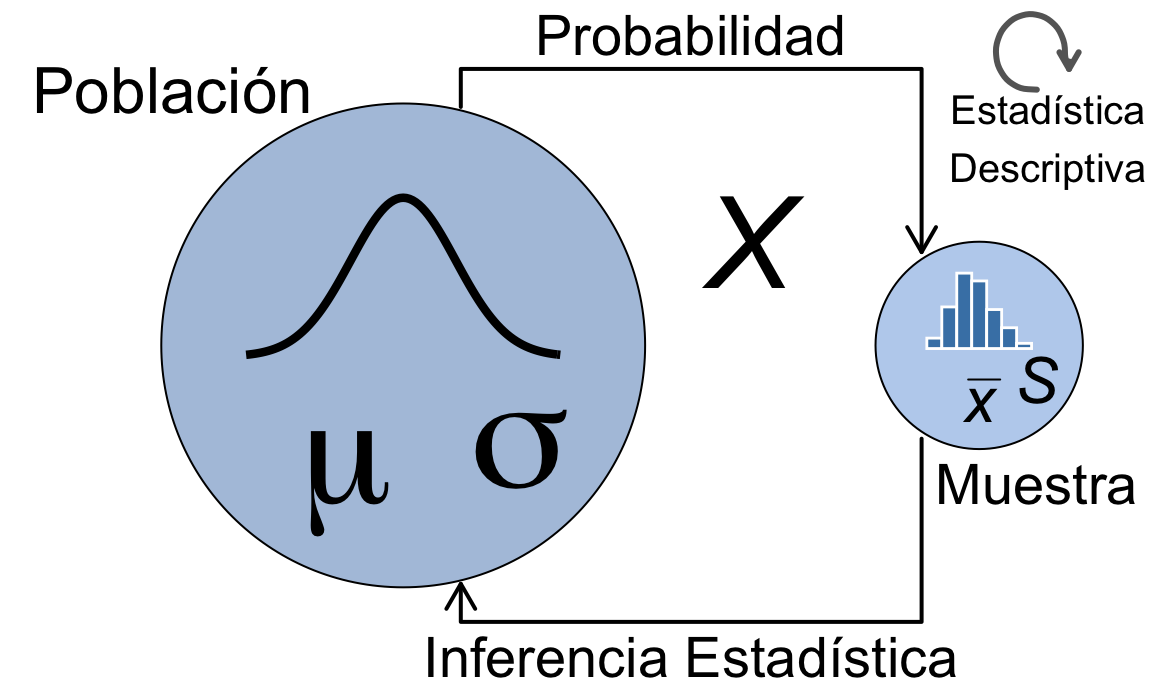
\includegraphics[width=0.5\textwidth,height=\textheight]{dogma2.png}

}

\caption{\label{fig-muestreo2}Parámetros vs.~Estadísticos}

\end{figure}

Es decir, una vez obtenida una muestra, es necesario extraer información
útil de la misma. Esto se hace a través de los estadístico.

Diremos que un estadístico \(T= T(x_1,\ldots,x_n)\) es una función real
de la muestra aleatoria \((x_1,\ldots,x_n)\).

Un estadístico es una variable aleatoria, y por lo tanto, tiene asociada
una distribución. La ditribución de probabilidad correspondiente a un
estadístico se denomina \textbf{distribución muestral}.

Por ejemplo, sea \((X_1,\ldots,X_n)\) una muestra aletoria de una
población \(X\) con esperanza \(\mu\) y vaianza \(\sigma^2\).
Consideremos los siguientes ejemplos de estadísticos:

\begin{itemize}
\tightlist
\item
  \textbf{Media Muestral} (\(\bar{X}\)): Utilizada para estimar la media
  poblacional. \[
  \bar{X}=\frac{1}{n}\sum_{i=1}^nX_i
  \]
\item
  \textbf{Varianza Muestral} (\(V\)): Utilizada para estimar la varianza
  poblacional. \[
  V=\frac{1}{n}\sum_{i=1}^n(X_i-\bar{X})^2
  \]
\item
  \textbf{Cuasivarianza muestral} (\(S^2\)) \[
  S^2=\frac{1}{n-1}\sum_{i=1}^n(X_i-\bar{X})^2=\frac{1}{n-1}\left [ \sum_{i=1}^nX_i^2-n\bar{X}^2\right]
  \] Entonces se tienen las siguientes propiedades:
\end{itemize}

\[
E(\bar{X})=\mu
\] \[
Var(\bar{X})=\frac{\sigma^2}{n}
\]

\[
E(V)=\frac{n-1}{n}\sigma^2
\] \[
E(S^2)=\sigma^2
\]

\hypertarget{uso-de-la-muestra}{%
\subsection{Uso de la muestra}\label{uso-de-la-muestra}}

Supongamos que queremos estudiar una característica de cierta población.
Est característica se representa mediante una variable aleatoria \(X\) y
el estudio se centra en su valor medio \(E[X]\). Para ello, se decide
tomar una muestra y se obtiene un estadístico, la \emph{media muestral},
que se utiliza para estimar el valor de \(E[X]\): \[
\bar{X}=\frac{1}{n}\sum_{i=1}^nX_i
\] Fíjate que este estadístico \(\bar{X}\) es una variable aleatoria.
Una vez tomada una muestra particular \((x_1,\ldots,x_n)\) de la
variable aleatoria \(X\) se obtiene un valor numérico particular para la
variable aleatoria \(\bar{X}\): \[
\bar{x}=\frac{1}{n}\sum_{i=1}^nx_i
\]

\begin{tcolorbox}[enhanced jigsaw, arc=.35mm, breakable, coltitle=black, left=2mm, opacityback=0, bottomtitle=1mm, colbacktitle=quarto-callout-important-color!10!white, title=\textcolor{quarto-callout-important-color}{\faExclamation}\hspace{0.5em}{Para recordar}, titlerule=0mm, colback=white, colframe=quarto-callout-important-color-frame, bottomrule=.15mm, rightrule=.15mm, opacitybacktitle=0.6, toptitle=1mm, toprule=.15mm, leftrule=.75mm]

\[\bar{X}\neq\bar{x}\]

\end{tcolorbox}

\begin{tcolorbox}[enhanced jigsaw, arc=.35mm, breakable, coltitle=black, left=2mm, opacityback=0, bottomtitle=1mm, colbacktitle=quarto-callout-tip-color!10!white, title=\textcolor{quarto-callout-tip-color}{\faLightbulb}\hspace{0.5em}{Ejemplo. Diferencia entre parámetro y estadístico}, titlerule=0mm, colback=white, colframe=quarto-callout-tip-color-frame, bottomrule=.15mm, rightrule=.15mm, opacitybacktitle=0.6, toptitle=1mm, toprule=.15mm, leftrule=.75mm]

Se quiere estudiar la temperatura de una solución líquida en un
labortorio y conocer el valor medio \(\mu\) (parámetro de la población),
que es desconocido. Se supone que la temperatura se puede aproximar
mediante una variable aleatoria de la que se desconoce su distribución.
Una opción razonable para estimarla sería escoger una muestra de la
solución, medir su temperatura, y estimar \(\mu\) mediante el promedio
de esa muestra (estadístico muestral): \[ \hat{\mu}=\bar{X}\] Es
importante señalar que podríamo emplear otros estadísticos diferentes.

Supongamos ahora que se toma una muestra de 10 mediciones de temperatura
de dicha solución, obteniendo estos valores:

\begin{verbatim}
 [1] 45.76 42.75 45.54 49.61 53.00 44.15 51.48 48.69 51.33 49.21
\end{verbatim}

Siendo su valor promedio \(\bar{x}=\) 48.15. Este valor estima el
verdadero valor desconocido del parámetro \(\mu\).

Ahora, supongamos que se toma otra muestra de 5 mediciones de
temperatura de dicha solución, obteniendo estos valores:

\begin{verbatim}
[1] 50.18 43.89 46.18 47.74 46.59
\end{verbatim}

La media de esta otra muestra es \(\bar{x}=\) 46.92 otra estimación del
desconocido valor del parámetro \(\mu\).

¿Cuál de las dos estimaciones te parece más fiable? ¿Por qué? ¿Cómo
podríamos ``asegurar'' que nuestro estimar es altamente fiable?

Repetimos el primer experimento \(100\) días consecutivos. Es decir,
tomamos \(10\) muestras de tamaño 10 y estimamos, para cada muestra el
valor del parámetro \(\mu\) mediante la media muestral. El siguiente
gráfico muestra los valores de esas \(100\) muestras:

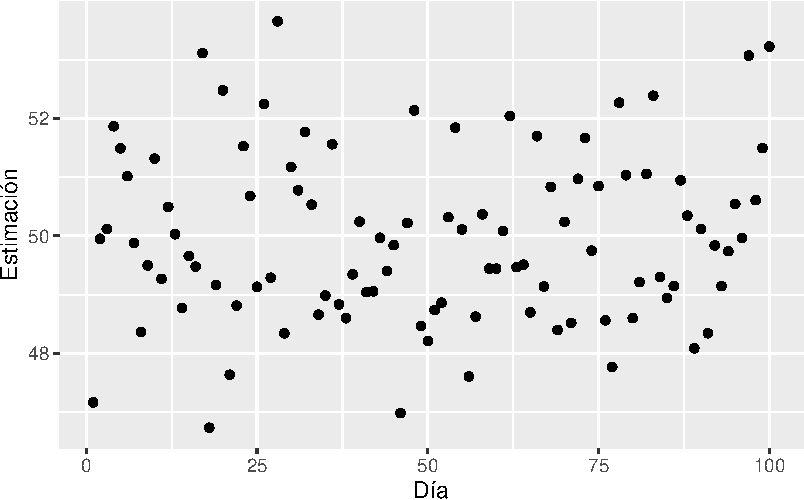
\includegraphics{intro_files/figure-pdf/sample3-1.pdf}

¿Cuál es, a tu juicio, un buen valor del estimador del parámetro?
Supongamos que tu profesor ha simulado estos datos. Es decir, tu
profesor \emph{conoce} realmente el \emph{verdadero} valor del
parámetro. En ese caso, te propone el siguiente reto: Dame dos valores
(uno bajo y otro alto) entre los cuales crees que está el verdadero
valor que solo yo (el profesor) conozco. ¿Qué valores darías? Te propone
un reto mayor: ¿Qué valores darías si quisieras estar seguro al \(100%
\) de acertar? Es decir, que la probabilidad de fallo sea \(0\).

\end{tcolorbox}

\hypertarget{estaduxedstica-paramuxe9trica-y-no-paramuxe9trica}{%
\section{Estadística paramétrica y no
paramétrica}\label{estaduxedstica-paramuxe9trica-y-no-paramuxe9trica}}

Tal y como hemos visto hasta ahora, el objetivo general de la inferencia
es obtener información acerca de la distribución de una variable
aleatoria \(X\) mediante la observación de una muestra
\((X_1,\ldots,X_n)\). En este curso vamos a tratar con dos tipos de
herramientas para realizar inferencia estadística: la estadística
paramétrica y la no paramétrica. Veamos sus semejanzas y diferencias:

\textbf{Estadística Paramétrica}

La estadística paramétrica se basa en la suposición de que los datos
siguen una distribución conocida, como la distribución normal, binomial,
Poisson, etc. Estas suposiciones (o hipótesis) deben ser comprobadas
para dar validez a este tipo de pruebas. Los parámetros de estas
distribuciones, como la media y la varianza, se utilizan para resumir la
información de los datos y realizar inferencias.

\begin{tcolorbox}[enhanced jigsaw, arc=.35mm, breakable, coltitle=black, left=2mm, opacityback=0, bottomtitle=1mm, colbacktitle=quarto-callout-tip-color!10!white, title=\textcolor{quarto-callout-tip-color}{\faLightbulb}\hspace{0.5em}{Familias paramétricas}, titlerule=0mm, colback=white, colframe=quarto-callout-tip-color-frame, bottomrule=.15mm, rightrule=.15mm, opacitybacktitle=0.6, toptitle=1mm, toprule=.15mm, leftrule=.75mm]

Se tiene una variable aleatoria \(X\) cuya distribución se supone
perteneciente a una cierta familia paramétrica \{\(f_\theta\)\} donde
\(\theta \in \Theta\).

La distribución de \(X\) es conocida excepto por el valor del parámetro
\(\theta\), del cual lo único que se conoce es su rango de posibles
valores, \(\Theta\), denominado espacio parémtrico.

\textbf{Ejemplos de familias paramétricas}

\begin{itemize}
\tightlist
\item
  \(X \sim N(\mu,\sigma^2) \rightarrow \theta=(\mu,\sigma^2)\)
\item
  \(X \sim Bernoulli(p) \rightarrow \theta=p\)
\item
  \(X \sim Exp(\lambda) \rightarrow \theta=\lambda\)
\end{itemize}

\end{tcolorbox}

Por tanto, el objeto de los métodos paramétricos es obtener información
sobre el parámetro de interés mediante la obtención de muestras de la
variable aleatoria.

Los métodos paramétricos son más potentes que los no paramétricos (es
decir, tienen una mayor probabilidad de detectar un efecto verdadero) si
las suposiciones son correctas. Ejemplos de pruebas paramétricas
incluyen la prueba \emph{t de Student}, el \emph{análisis de varianza
(ANOVA)} y la \emph{regresión lineal} que veréis en el segundo
cuatrimestre.

\textbf{Estadística No Paramétrica}

La estadística no paramétrica no hace suposiciones fuertes sobre la
distribución de los datos. Estos métodos son más flexibles y robustos a
las violaciones de las suposiciones, pero pueden ser menos potentes si
las suposiciones de los métodos paramétricos son verdaderas. Los métodos
no paramétricos a menudo se basan en el orden de los datos, en lugar de
sus valores exactos. Ejemplos de pruebas no paramétricas incluyen la
prueba de \emph{Mann-Whitney U}, la prueba de \emph{Kruskal-Wallis} y la
prueba de \emph{Chi-cuadrado}.

La elección entre métodos paramétricos y no paramétricos depende de la
naturaleza de tus datos y de las suposiciones que estés dispuesto a
hacer. Si tus datos cumplen con las suposiciones de una prueba
paramétrica, esa prueba puede ser la opción más potente. Si no, una
prueba no paramétrica puede ser más apropiada.

\hypertarget{frecuentistas-vs-bayesianos}{%
\section{Frecuentistas vs
Bayesianos}\label{frecuentistas-vs-bayesianos}}

En el campo de la estadística existen dos enfoques diferentes que han de
ser comentados, la inferencia clásica (o frecuentista) y la inferencia
Bayesiana.

\textbf{Enfoque Frecuentista}

Los frecuentistas interpretan la probabilidad como la frecuencia
relativa de un evento en un número infinito de repeticiones del
experimento. Se obtienen datos a través de una muestra y con técnicas
estadísticas se extrae informaión de los mismos mediante, los llamados,
estimadores. En base a esas estimaciones se toman decisiones en el
dominio de aplicación.

Los métodos frecuentistas son ampliamente utilizados y son la base de
muchas técnicas estadísticas clásicas. Los parámetros son considerados
como valores fijos y desconocidos que se estiman a partir de los datos.
Los intervalos de confianza, que veremos más adelante, se interpretan en
términos de repetibilidad: si se repite el experimento muchas veces, el
intervalo de confianza capturará el verdadero parámetro en un porcentaje
dado de las veces. Esta interpretación es un poco \emph{extraña} para el
no iniciado y trataremos de explicarlo en detalle en capítulos
posteriores.

\textbf{Enfoque Bayesiano}

La inferencia Bayesiana tiene su fundamento en el teorema de Bayes. El
teorema de Bayes, también conocido como regla de Bayes, es un principio
fundamental en la teoría de la probabilidad que describe la forma de
actualizar las probabilidades de una hipótesis basándose en nueva
evidencia o información. Fue formulado por el matemático británico
Thomas Bayes en el siglo XVIII. Probablemente hayas estudiado este
teorema en asignaturas anterires del grado. En cualquier caso, es
sencillo y dice así:

\[
P(A|B) = \frac{P(B|A) \cdot P(A)}{P(B)}
\]

donde:

\begin{itemize}
\tightlist
\item
  \(P(A|B)\) es la probabilidad de que ocurra el evento \(A\) dado que
  ha ocurrido el evento \(B\). Esta es conocida como la
  \textbf{probabilidad a posteriori}.
\item
  \(P(B|A)\) es la probabilidad de que ocurra el evento \(B\) dado que
  ha ocurrido el evento \(A\). Esta es conocida como la
  \textbf{probabilidad verosímil} o \textbf{likelihood}.
\item
  \(P(A)\) es la probabilidad de que ocurra el evento \(A\) sin ninguna
  información adicional sobre \(B\). Esta es conocida como la
  \textbf{probabilidad a priori} o simplemente la \textbf{probabilidad
  previa}.
\item
  \(P(B)\) es la probabilidad de que ocurra el evento \(B\) bajo todas
  las posibles hipótesis. Esta es conocida como la \textbf{probabilidad
  marginal} de \(B\).
\end{itemize}

Vemos que el teorema de Bayes permite actualizar la probabilidad de una
hipótesis \(A\) a la luz de nueva evidencia \(B\). Básicamente,
proporciona una forma de ajustar nuestras creencias iniciales
(probabilidad a priori) en base a la nueva información disponible
(evidencia).

\begin{tcolorbox}[enhanced jigsaw, arc=.35mm, breakable, coltitle=black, left=2mm, opacityback=0, bottomtitle=1mm, colbacktitle=quarto-callout-tip-color!10!white, title=\textcolor{quarto-callout-tip-color}{\faLightbulb}\hspace{0.5em}{Ejemplo. Teorema de Bayes.}, titlerule=0mm, colback=white, colframe=quarto-callout-tip-color-frame, bottomrule=.15mm, rightrule=.15mm, opacitybacktitle=0.6, toptitle=1mm, toprule=.15mm, leftrule=.75mm]

Imaginemos que estamos tratando de diagnosticar una enfermedad rara que
afecta al \(1\%\) de la población \((P(\text{Enfermedad}) = 0.01\).
Existe una prueba para esta enfermedad que es \(99\%\) precisa:

\begin{itemize}
\tightlist
\item
  Si una persona tiene la enfermedad, la prueba es positiva el \(99\%\)
  de las veces, es decir
  \(P(\text{Positivo}|\text{Enfermedad}) = 0.99\).
\item
  Si una persona no tiene la enfermedad, la prueba es negativa el
  \(99\%\) de las veces
  \(P(\text{Negativo}|\text{No Enfermedad}) = 0.99\), lo que significa
  que tiene un \(1\%\) de falsos positivos
  \(P(\text{Positivo}|\text{No Enfermedad}) = 0.01\).
\end{itemize}

En este caso, deseamos saber cuál es la probabilidad de que una persona
tenga la enfermedad si la prueba ha sido positiva
\(P(\text{Enfermedad}|\text{Positivo}\).

Aplicamos el teorema de Bayes:

\[
P(\text{Enfermedad}|\text{Positivo}) = \frac{P(\text{Positivo}|\text{Enfermedad}) \cdot P(\text{Enfermedad})}{P(\text{Positivo})}
\]

Primero, calculamos \(P(\text{Positivo})\), la probabilidad total de que
la prueba sea positiva:

\[
P(\text{Positivo}) = P(\text{Positivo}|\text{Enfermedad}) \cdot P(\text{Enfermedad}) +
\]
\[P(\text{Positivo}|\text{No Enfermedad}) \cdot P(\text{No Enfermedad})
\]

\[
P(\text{Positivo}) = (0.99 \times 0.01) + (0.01 \times 0.99) = 0.0099 + 0.0099 = 0.0198
\]

Ahora, aplicamos el teorema de Bayes:

\[
P(\text{Enfermedad}|\text{Positivo}) = \frac{0.99 \times 0.01}{0.0198} = \frac{0.0099}{0.0198} \approx 0.50
\]

Esto significa que, a pesar de que la prueba es bastante precisa, si una
persona da positivo en la prueba, la probabilidad de que realmente tenga
la enfermedad es aproximadamente \(50\%\), debido a la baja prevalencia
de la enfermedad en la población.

\end{tcolorbox}

El teorema de Bayes es una herramienta poderosa para la toma de
decisiones y la inferencia estadística, ya que proporciona un marco
formal para actualizar nuestras creencias en base a la evidencia
disponible.

Los bayesianos interpretan la probabilidad como una medida de la
creencia o confianza en un evento. Esta creencia puede ser actualizada a
medida que se obtiene más información. Los parámetros son considerados
como variables aleatorias y se describe su incertidumbre a través de
distribuciones de probabilidad. Los intervalos de credibilidad
bayesianos proporcionan una medida directa de la incertidumbre del
parámetro: hay una probabilidad dada de que el verdadero parámetro esté
dentro del intervalo de credibilidad. Esto parece tener más
\emph{lógica} que el enfoque frecuentista, pero es menos habitual. Los
métodos bayesianos permiten la incorporación directa de conocimientos
previos en el análisis a través de la distribución a priori.

Por tanto, la principal diferencia entre los enfoques frecuentista y
bayesiano radica en cómo interpretan el concepto de probabilidad. El
enfoque frecuentista se basa en frecuencias de eventos, mientras que el
enfoque bayesiano se basa en la incertidumbre y la actualización de las
creencias.

\hypertarget{notaciuxf3n}{%
\section{Notación}\label{notaciuxf3n}}

A lo largo de este libro vamos a usar la siguiente notación:

\begin{itemize}
\item
  \(X, Y\): Variables
\item
  \(i\): Identificador o índice para cada observación o clase
\item
  \(x_i\): Valor que toma la variable \(X\) en la observación \(i\)
\item
  \(c_i\): Marca de clase en datos agrupados
\item
  \(n\): Número total de observaciones
\item
  \(k\): Número de clases
\item
  \(n_i\): Número de observaciones en la clase \(i\)
\item
  \(\bar{x}\): Media muestral de la variable \(X\)
\item
  \(s^2\): Varianza muestral de la variable \(X\)
\item
  \(s\): Desviación típica muestral de la variable \(X\)
\item
  \(\mu\): Media poblacional
\item
  \(\sigma^2\): Varianza poblacional
\item
  \(\hat{[\cdot]}\): Simboliza un estimador de \(\cdot\). Por ejemplo,
  \(s = \hat{\sigma}\) quiere decir que la desviación típica muestral
  \(s\) es un estimador de la desviación típica poblacional \(\sigma\).
  {]}
\end{itemize}

\hypertarget{resuxfamenes-gruxe1ficas-y-numuxe9ricas-uxfatiles-en-la-inferencia-estaduxedstica}{%
\section{Resúmenes gráficas y numéricas útiles en la inferencia
estadística}\label{resuxfamenes-gruxe1ficas-y-numuxe9ricas-uxfatiles-en-la-inferencia-estaduxedstica}}

\hypertarget{muxe9todos-numuxe9ricos}{%
\subsection{Métodos numéricos}\label{muxe9todos-numuxe9ricos}}

Tal y como hemos indicado anteriormente, los métodos numéricos de
inferencia estadística son técnicas y procedimientos utilizados para
analizar datos y hacer inferencias sobre una población a partir de una
muestra. Estos métodos se apoyan en herramientas matemáticas y
computacionales para estimar parámetros, evaluar hipótesis y tomar
decisiones informadas. A continuación, se describen los principales
métodos numéricos en la inferencia estadística. No tienes que
aprenderlos ahora puesto que vamos a trabajar con estos métodos a lo
largo de todo el curso. Los veremos con mayor detalle en los próximos
capítulos.

\begin{tcolorbox}[enhanced jigsaw, arc=.35mm, breakable, coltitle=black, left=2mm, opacityback=0, bottomtitle=1mm, colbacktitle=quarto-callout-note-color!10!white, title=\textcolor{quarto-callout-note-color}{\faInfo}\hspace{0.5em}{Estimación puntual}, titlerule=0mm, colback=white, colframe=quarto-callout-note-color-frame, bottomrule=.15mm, rightrule=.15mm, opacitybacktitle=0.6, toptitle=1mm, toprule=.15mm, leftrule=.75mm]

La \textbf{estimación puntual} implica el uso de un solo valor
estadístico de la muestra para estimar un parámetro de la población.

\begin{itemize}
\tightlist
\item
  \textbf{Media Muestral (}\(\bar{x}\)): Utilizada para estimar la media
  poblacional (\(\mu\)).
\item
  \textbf{Proporción Muestral (}\(\hat{p}\)): Utilizada para estimar la
  proporción poblacional (\(p\)).
\item
  \textbf{Varianza Muestral (}\(s^2\)): Utilizada para estimar la
  varianza poblacional (\(\sigma^2\)).
\end{itemize}

\end{tcolorbox}

\begin{tcolorbox}[enhanced jigsaw, arc=.35mm, breakable, coltitle=black, left=2mm, opacityback=0, bottomtitle=1mm, colbacktitle=quarto-callout-note-color!10!white, title=\textcolor{quarto-callout-note-color}{\faInfo}\hspace{0.5em}{Estimación por intervalo}, titlerule=0mm, colback=white, colframe=quarto-callout-note-color-frame, bottomrule=.15mm, rightrule=.15mm, opacitybacktitle=0.6, toptitle=1mm, toprule=.15mm, leftrule=.75mm]

La \textbf{estimación por intervalo} proporciona un rango de valores
dentro del cual se espera que se encuentre el parámetro poblacional con
un cierto nivel de confianza.

\begin{itemize}
\tightlist
\item
  \textbf{Intervalo de confianza para la media}:

  \begin{itemize}
  \tightlist
  \item
    Para muestras grandes (\(n \ge 30\)):
    \(\bar{x} \pm Z_{\alpha/2} \left(\frac{\sigma}{\sqrt{n}}\right )\)\\
  \item
    Para muestras pequeñas (\(n < 30\)) y cuando la distribución es
    normal:
    \(\bar{x} \pm t_{\alpha/2, n-1} \left(\frac{s}{\sqrt{n}}\right)\)
  \end{itemize}
\item
  \textbf{Intervalo de confianza para la proporción}:
  \(\hat{p} \pm Z_{\alpha/2} \sqrt{\frac{\hat{p}(1-\hat{p})}{n}}\)
\item
  \textbf{Intervalo de confianza para la varianza}:
  \(\left( \frac{(n-1)s^2}{\chi^2_{\alpha/2, n-1}}, \frac{(n-1)s^2}{\chi^2_{1-\alpha/2, n-1}} \right)\)
\end{itemize}

\end{tcolorbox}

\begin{tcolorbox}[enhanced jigsaw, arc=.35mm, breakable, coltitle=black, left=2mm, opacityback=0, bottomtitle=1mm, colbacktitle=quarto-callout-note-color!10!white, title=\textcolor{quarto-callout-note-color}{\faInfo}\hspace{0.5em}{Contraste de hipótesis}, titlerule=0mm, colback=white, colframe=quarto-callout-note-color-frame, bottomrule=.15mm, rightrule=.15mm, opacitybacktitle=0.6, toptitle=1mm, toprule=.15mm, leftrule=.75mm]

El \textbf{contraste de hipótesis} es un procedimiento para tomar
decisiones sobre los parámetros poblacionales basándose en la evidencia
proporcionada por los datos muestrales.

\begin{itemize}
\item
  \textbf{Formulación de hipótesis}:

  \begin{itemize}
  \item
    Hipótesis nula (\(H_0\)): Es la afirmación que se desea probar o
    refutar.
  \item
    Hipótesis alternativa (\(H_1\)): Es la afirmación que se acepta si
    se rechaza (\(H_0\)).
  \end{itemize}
\item
  \textbf{Pruebas para la media}:

  \begin{itemize}
  \item
    \textbf{Prueba Z}: Utilizada para muestras grandes (\(n \ge 30\)) o
    cuando se conoce la desviación estándar poblacional (\(\sigma\)).
  \item
    \textbf{Prueba t}: Utilizada para muestras pequeñas (\(n < 30\)) y
    cuando no se conoce (\(\sigma\)).
  \end{itemize}
\item
  \textbf{Pruebas para la proporción}:

  \begin{itemize}
  \tightlist
  \item
    \textbf{Prueba Z para proporciones}: Utilizada para evaluar
    hipótesis sobre una proporción poblacional.
  \end{itemize}
\item
  \textbf{Pruebas para la Varianza}:

  \begin{itemize}
  \tightlist
  \item
    \textbf{Prueba Chi-cuadrado}: Utilizada para evaluar hipótesis sobre
    la varianza poblacional.
  \end{itemize}
\end{itemize}

\end{tcolorbox}

\begin{tcolorbox}[enhanced jigsaw, arc=.35mm, breakable, coltitle=black, left=2mm, opacityback=0, bottomtitle=1mm, colbacktitle=quarto-callout-note-color!10!white, title=\textcolor{quarto-callout-note-color}{\faInfo}\hspace{0.5em}{Métodos de resampling}, titlerule=0mm, colback=white, colframe=quarto-callout-note-color-frame, bottomrule=.15mm, rightrule=.15mm, opacitybacktitle=0.6, toptitle=1mm, toprule=.15mm, leftrule=.75mm]

Los métodos de resampling, como el \textbf{bootstrap} y el
\textbf{jackknife}, son técnicas computacionales utilizadas para estimar
la precisión de los estadísticos de la muestra.

\begin{itemize}
\item
  \textbf{Bootstrap}: Consiste en tomar múltiples muestras con reemplazo
  de los datos originales y calcular el estadístico de interés para cada
  muestra. Esto permite construir una distribución empírica del
  estadístico y estimar intervalos de confianza.
\item
  \textbf{Jackknife}: Involucra excluir sistemáticamente cada
  observación de la muestra y recalcular el estadístico de interés. Esto
  proporciona una manera de estimar el sesgo y la varianza del
  estimador.
\end{itemize}

\end{tcolorbox}

\begin{tcolorbox}[enhanced jigsaw, arc=.35mm, breakable, coltitle=black, left=2mm, opacityback=0, bottomtitle=1mm, colbacktitle=quarto-callout-note-color!10!white, title=\textcolor{quarto-callout-note-color}{\faInfo}\hspace{0.5em}{Métodos bayesianos}, titlerule=0mm, colback=white, colframe=quarto-callout-note-color-frame, bottomrule=.15mm, rightrule=.15mm, opacitybacktitle=0.6, toptitle=1mm, toprule=.15mm, leftrule=.75mm]

La inferencia bayesiana utiliza la probabilidad subjetiva para
actualizar la creencia sobre los parámetros poblacionales basándose en
la evidencia muestral.

\begin{itemize}
\tightlist
\item
  \textbf{Teorema de Bayes}:
  \(P( \theta |x) = \frac{P(x | \theta)P( \theta)}{P(x)}\), donde
  \(P(\theta|x)\) es la distribución a posteriori, \(P(x|\theta)\) es la
  verosimilitud, \(P(\theta)\) es la distribución a priori y \(P(x)\) es
  la probabilidad marginal de los datos.
\item
  \textbf{Simulación Monte Carlo Markov Chain (MCMC)}: Es un método
  numérico para aproximar distribuciones posteriores complejas.
\end{itemize}

\end{tcolorbox}

\begin{tcolorbox}[enhanced jigsaw, arc=.35mm, breakable, coltitle=black, left=2mm, opacityback=0, bottomtitle=1mm, colbacktitle=quarto-callout-note-color!10!white, title=\textcolor{quarto-callout-note-color}{\faInfo}\hspace{0.5em}{Pruebas no paramétricas}, titlerule=0mm, colback=white, colframe=quarto-callout-note-color-frame, bottomrule=.15mm, rightrule=.15mm, opacitybacktitle=0.6, toptitle=1mm, toprule=.15mm, leftrule=.75mm]

Cuando no se cumplen los supuestos de normalidad, se utilizan pruebas no
paramétricas que no requieren asumir una distribución específica.

\begin{itemize}
\tightlist
\item
  \textbf{Prueba de Wilcoxon}: Para comparar medianas entre dos muestras
  emparejadas.
\item
  \textbf{Prueba de Mann-Whitney}: Para comparar medianas entre dos
  muestras independientes.
\item
  \textbf{Prueba de Kruskal-Wallis}: Extensión de la prueba de
  Mann-Whitney para más de dos grupos.
\item
  \textbf{Prueba de Chi-cuadrado}: Para pruebas de independencia y
  homogeneidad en tablas de contingencia.
\end{itemize}

\end{tcolorbox}

\hypertarget{muxe9todos-gruxe1ficos}{%
\subsection{Métodos gráficos}\label{muxe9todos-gruxe1ficos}}

A lo largo del curso usaremos numerosos métodos gráficos para explorar
los datos dentro del contexto de la inferencia estadística. Algunas de
los métodos básicos son:

\begin{tcolorbox}[enhanced jigsaw, arc=.35mm, breakable, coltitle=black, left=2mm, opacityback=0, bottomtitle=1mm, colbacktitle=quarto-callout-note-color!10!white, title=\textcolor{quarto-callout-note-color}{\faInfo}\hspace{0.5em}{Histogramas}, titlerule=0mm, colback=white, colframe=quarto-callout-note-color-frame, bottomrule=.15mm, rightrule=.15mm, opacitybacktitle=0.6, toptitle=1mm, toprule=.15mm, leftrule=.75mm]

Gráficos de barras que muestran la distribución de frecuencias de datos
cuantitativos.

\end{tcolorbox}

\begin{tcolorbox}[enhanced jigsaw, arc=.35mm, breakable, coltitle=black, left=2mm, opacityback=0, bottomtitle=1mm, colbacktitle=quarto-callout-note-color!10!white, title=\textcolor{quarto-callout-note-color}{\faInfo}\hspace{0.5em}{Gráficos de caja (boxplots)}, titlerule=0mm, colback=white, colframe=quarto-callout-note-color-frame, bottomrule=.15mm, rightrule=.15mm, opacitybacktitle=0.6, toptitle=1mm, toprule=.15mm, leftrule=.75mm]

Muestran la mediana, los cuartiles y los posibles valores atípicos.

\end{tcolorbox}

\begin{tcolorbox}[enhanced jigsaw, arc=.35mm, breakable, coltitle=black, left=2mm, opacityback=0, bottomtitle=1mm, colbacktitle=quarto-callout-note-color!10!white, title=\textcolor{quarto-callout-note-color}{\faInfo}\hspace{0.5em}{Gráficos de dispersión (scatterplots)}, titlerule=0mm, colback=white, colframe=quarto-callout-note-color-frame, bottomrule=.15mm, rightrule=.15mm, opacitybacktitle=0.6, toptitle=1mm, toprule=.15mm, leftrule=.75mm]

Utilizados para observar la relación entre dos variables cuantitativas.

\end{tcolorbox}

\hypertarget{teorema-central-del-luxedmite}{%
\section{Teorema Central del
Límite}\label{teorema-central-del-luxedmite}}

El Teorema Central del Límite (TCL) es uno de los principios más
fundamentales en la estadística y la probabilidad. Establece que, bajo
ciertas condiciones, la distribución de la suma (o el promedio) de un
gran número de variables aleatorias independientes e identicamente
distribuidas tiende a seguir una distribución Normal, independientemente
de la distribución original de las variables.

Formalmente, el TCL establece que si, \(X_1,X_2,\ldots,X_n\) son
variables aleatorias independientes e idénticamente distribuidas, con
media \(\mu\) y varianza \(\sigma^2<\infty\), entonces, para \(n\)
suficientemente grande se verifica:

\[\bar{X} \approx N \left ( \mu,\frac{\sigma^2}{n}\right )\] Este
resultado es válido tanto para variables discretas como continuas, sean
simétricas o asimétricas, unimodales o multimodales.

\begin{tcolorbox}[enhanced jigsaw, arc=.35mm, breakable, coltitle=black, left=2mm, opacityback=0, bottomtitle=1mm, colbacktitle=quarto-callout-important-color!10!white, title=\textcolor{quarto-callout-important-color}{\faExclamation}\hspace{0.5em}{Para recordar}, titlerule=0mm, colback=white, colframe=quarto-callout-important-color-frame, bottomrule=.15mm, rightrule=.15mm, opacitybacktitle=0.6, toptitle=1mm, toprule=.15mm, leftrule=.75mm]

El Teorema Central del Límite asegura que con muestas suficientemente
grandes se pueden utilizar estimaciones basadas en la distribución
Normal independientemente del tipo de distribución que siga la variable
que nos interesa.

\end{tcolorbox}

\begin{tcolorbox}[enhanced jigsaw, arc=.35mm, breakable, coltitle=black, left=2mm, opacityback=0, bottomtitle=1mm, colbacktitle=quarto-callout-tip-color!10!white, title=\textcolor{quarto-callout-tip-color}{\faLightbulb}\hspace{0.5em}{Ejemplo. Teorema Central del Límite}, titlerule=0mm, colback=white, colframe=quarto-callout-tip-color-frame, bottomrule=.15mm, rightrule=.15mm, opacitybacktitle=0.6, toptitle=1mm, toprule=.15mm, leftrule=.75mm]

Acabamos de ver que el TCL establece que, para una gran cantidad de
muestras aleatorias tomadas de una población con una distribución
cualquiera (con una media y una varianza finitas), la distribución de
las medias muestrales tiende a ser Normal, independientemente de la
forma de la distribución original.

Aquí tienes un ejemplo en R que ilustra el Teorema Central del Límite.
Vamos a tomar muestras de una distribución no normal (por ejemplo, una
distribución uniforme). Calcularemos las medias de estas muestras y
observaremos cómo las medias muestrales se aproximan a una distribución
normal.

\begin{Shaded}
\begin{Highlighting}[]
\CommentTok{\# Configuraciones iniciales}
\FunctionTok{set.seed}\NormalTok{(}\DecValTok{123}\NormalTok{)          }\CommentTok{\# Fijamos la semilla para reproducibilidad}
\NormalTok{n\_samples }\OtherTok{\textless{}{-}} \DecValTok{1000}      \CommentTok{\# Número de muestras}
\NormalTok{sample\_size }\OtherTok{\textless{}{-}} \DecValTok{30}      \CommentTok{\# Tamaño de cada muestra}

\CommentTok{\# Generamos las muestras de una distribución uniforme}
\NormalTok{sample\_means }\OtherTok{\textless{}{-}} \FunctionTok{numeric}\NormalTok{(n\_samples)}
\ControlFlowTok{for}\NormalTok{ (i }\ControlFlowTok{in} \DecValTok{1}\SpecialCharTok{:}\NormalTok{n\_samples) \{}
\NormalTok{  sample }\OtherTok{\textless{}{-}} \FunctionTok{runif}\NormalTok{(sample\_size, }\AttributeTok{min =} \DecValTok{0}\NormalTok{, }\AttributeTok{max =} \DecValTok{10}\NormalTok{)}
\NormalTok{  sample\_means[i] }\OtherTok{\textless{}{-}} \FunctionTok{mean}\NormalTok{(sample)}
\NormalTok{\}}

\CommentTok{\# Crear un data frame con las medias muestrales}
\NormalTok{data }\OtherTok{\textless{}{-}} \FunctionTok{data.frame}\NormalTok{(sample\_means)}

\CommentTok{\# Graficamos el histograma de las medias muestrales utilizando ggplot2}
\FunctionTok{ggplot}\NormalTok{(data, }\FunctionTok{aes}\NormalTok{(}\AttributeTok{x =}\NormalTok{ sample\_means)) }\SpecialCharTok{+}
  \FunctionTok{geom\_histogram}\NormalTok{(}\FunctionTok{aes}\NormalTok{(}\AttributeTok{y =}\NormalTok{ ..density..), }\AttributeTok{bins =} \DecValTok{30}\NormalTok{, }\AttributeTok{fill =} \StringTok{"lightblue"}\NormalTok{, }\AttributeTok{color =} \StringTok{"black"}\NormalTok{) }\SpecialCharTok{+}
  \FunctionTok{stat\_function}\NormalTok{(}\AttributeTok{fun =}\NormalTok{ dnorm, }\AttributeTok{args =} \FunctionTok{list}\NormalTok{(}\AttributeTok{mean =} \FunctionTok{mean}\NormalTok{(sample\_means), }\AttributeTok{sd =} \FunctionTok{sd}\NormalTok{(sample\_means)),}
                \AttributeTok{color =} \StringTok{"red"}\NormalTok{, }\AttributeTok{size =} \DecValTok{1}\NormalTok{) }\SpecialCharTok{+}
  \FunctionTok{labs}\NormalTok{(}\AttributeTok{title =} \StringTok{"Distribución de las Medias Muestrales"}\NormalTok{,}
       \AttributeTok{x =} \StringTok{"Medias Muestrales"}\NormalTok{, }\AttributeTok{y =} \StringTok{"Densidad"}\NormalTok{) }\SpecialCharTok{+}
  \FunctionTok{theme\_minimal}\NormalTok{() }\SpecialCharTok{+}
  \FunctionTok{theme}\NormalTok{(}\AttributeTok{plot.title =} \FunctionTok{element\_text}\NormalTok{(}\AttributeTok{hjust =} \FloatTok{0.5}\NormalTok{)) }\SpecialCharTok{+}
  \FunctionTok{annotate}\NormalTok{(}\StringTok{"text"}\NormalTok{, }\AttributeTok{x =} \FunctionTok{mean}\NormalTok{(sample\_means), }\AttributeTok{y =} \FunctionTok{max}\NormalTok{(}\FunctionTok{density}\NormalTok{(sample\_means)}\SpecialCharTok{$}\NormalTok{y) }\SpecialCharTok{/} \DecValTok{2}\NormalTok{,}
           \AttributeTok{label =} \StringTok{"Distribución Normal"}\NormalTok{, }\AttributeTok{color =} \StringTok{"red"}\NormalTok{)}
\end{Highlighting}
\end{Shaded}

\begin{figure}[H]

{\centering 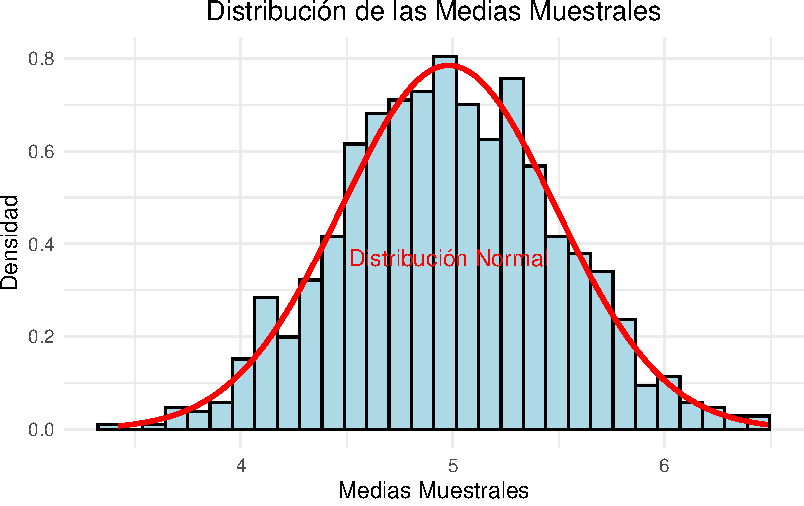
\includegraphics{intro_files/figure-pdf/TCL-1.pdf}

}

\end{figure}

Para visualizar el resultado, graficamos un histograma de las medias
muestrales. Luego, superponemos una curva de densidad de una
distribución normal con la misma media y desviación estándar que las
medias muestrales para observar cómo se ajusta a una distribución
normal.

El histograma de las medias muestrales se aproxima a una distribución
normal, a pesar de que las muestras originales provienen de una
distribución uniforme.

\end{tcolorbox}

\bookmarksetup{startatroot}

\hypertarget{sec-eda}{%
\chapter{Análisis Exploratorio de Datos}\label{sec-eda}}

En Chapter~\ref{sec-intro} hablamos de las dos ramas fundamentales de la
estadística:

\begin{itemize}
\item
  Estadística Descriptiva: buscamos una visión comprensible de los datos
  en base a resumir las características de un conjunto de datos mediante
  herramientas gráficas y numéricas.
\item
  Estadística Inferencial: utiliza muestras de datos para hacer
  generalizaciones o inferencias sobre una población más amplia.
\end{itemize}

La estadística descriptiva no solo proporciona las bases necesarias para
la inferencia estadística, sino que también juega un papel crucial en la
preparación, comprensión y comunicación de los datos. Para estudiantes
de Ciencia e Ingeniería de Datos, dominar estas herramientas es esencial
para poder aplicar técnicas inferenciales de manera correcta y efectiva.

\begin{itemize}
\item
  La estadística descriptiva proporciona las herramientas básicas
  necesarias para resumir y entender los datos. Sin una comprensión
  clara de cómo describir y resumir los datos, es difícil avanzar hacia
  métodos más complejos de inferencia estadística.
\item
  Las medidas descriptivas como la media, mediana, moda, varianza y
  desviación estándar son fundamentales para interpretar los resultados
  de las pruebas inferenciales.
\item
  Herramientas descriptivas como los gráficos (histogramas, diagramas de
  caja, gráficos de dispersión) ayudan a visualizar la distribución de
  los datos, detectar problemas y plantear hipótesis.
\item
  Sin una comprensión de la estadística descriptiva, los resultados de
  las pruebas inferenciales que estudiaremos en cap´itulos posteriores,
  pueden ser malinterpretados o exagerados. La interpretación de los
  resultados inferenciales se basa en la comprensión del contexto de los
  datos. Las estadísticas descriptivas proporcionan el contexto
  necesario para entender lo que los resultados inferenciales realmente
  significan.
\item
  Muchas técnicas de inferencia estadística se basan en ciertos
  supuestos sobre los datos (como la normalidad de las distribuciones,
  homogeneidad de varianzas, etc.). La estadística descriptiva permite
  verificar si estos supuestos se cumplen. Por ejemplo, se puede usar un
  histograma o un gráfico Q-Q para verificar la normalidad de los datos
  antes de aplicar una prueba t.
\end{itemize}

El análisis exploratorio de datos o (EDA, del inglés ``Exploratory Data
Analysis'') representa un conjunto de técnicas que permiten resumir los
aspectos más importantes de un conjunto de datos, normalmente con
especial énfasis en el uso de métodos de visualización gráfica. El
término fue popularizado, entre otros, por el estadístico norteamericano
\emph{John W. Tukey} como método para descubrir información importante
(y no evidente) contenida en los datos (Tukey et al. 1977). Estas
técnicas se emplean habitualmente como paso previo a la inferencia
estadística, orientada hacia un análisis confirmatorio. Así, con EDA se
estudian los datos, se descubre cómo son y cómo se comportan y con la
inferencia estadística se comprueba analíticamente si esos
comportamientos y diferencias halladas son realmente significativos
(desde un punto de vista estadístico). El EDA es, sin duda, fundamental
para adquirir conocimiento de los datos, antes de emplearlos dentro de
un modelo de ML como los que vais a aprendener a lo largo del grado en
Ciencia e Ingeniería de Datos. Es un error muy típico de algunos
analistas de datos aplicar modelos a sus datos en cuanto estos están
disponibles sin pasar previamente por el necesario análisis exploratorio
de los mismos.

\begin{tcolorbox}[enhanced jigsaw, arc=.35mm, breakable, coltitle=black, left=2mm, opacityback=0, bottomtitle=1mm, colbacktitle=quarto-callout-tip-color!10!white, title=\textcolor{quarto-callout-tip-color}{\faLightbulb}\hspace{0.5em}{John Tukey}, titlerule=0mm, colback=white, colframe=quarto-callout-tip-color-frame, bottomrule=.15mm, rightrule=.15mm, opacitybacktitle=0.6, toptitle=1mm, toprule=.15mm, leftrule=.75mm]

``El análisis exploratorio de datos es una actitud, un estado de
flexibilidad, una voluntad de buscar aquellas cosas que creemos que no
están ahí, así como aquellas que creemos que están ahí.''

\end{tcolorbox}

Es decir, el EDA no sigue un proceso formal con normas estrictas, algo
que sí suele ocurrir con la inferencia. Más bien, podemos decir que EDA
es una mentalidad o enfoque. En otras palabras, una forma de hacer las
cosas. Cuando lleves a cabo un EDA, debes sentirte libre para explorar
todas las ideas que se te ocurran. En inferencia, suele ocurrir que esas
ideas están planteadas a priori. Algunas de estas ideas serán
fructíferas, mientras que otras pueden llevarte a callejones sin salida.
No te preocupes, probablemente no hayas roto nada. Simplemente habrás
``gastado'' tiempo. A medida que sigas explorando, te enfocarás en áreas
particularmente prometedoras, las cuales documentarás y compartirás con
otros.

A menudo se necesita mucho tiempo para explorar los datos. Se dice que
el \emph{80\%} del tiempo del proyecto se gasta en EDA. A través del
proceso de EDA, podemos pedir que se redefina el enunciado del problema
o la definición de nuestro conjunto de datos, lo cual es muy importante.

\begin{tcolorbox}[enhanced jigsaw, arc=.35mm, breakable, coltitle=black, left=2mm, opacityback=0, bottomtitle=1mm, colbacktitle=quarto-callout-important-color!10!white, title=\textcolor{quarto-callout-important-color}{\faExclamation}\hspace{0.5em}{Para recordar}, titlerule=0mm, colback=white, colframe=quarto-callout-important-color-frame, bottomrule=.15mm, rightrule=.15mm, opacitybacktitle=0.6, toptitle=1mm, toprule=.15mm, leftrule=.75mm]

Cuando nos enfrentamos a un EDA, lo ideal es contar con un objetivo que
se haya definido junto con los datos, indicando qué se quiere conseguir
a partir de ellos. Por ejemplo, ``\emph{predecir las ventas en los
próximos 30 días}'', ``\emph{estimar el riesgo que tiene un paciente de
no superar una determinada operación quirúrgica}'', ``\emph{clasificar
como fraudulenta, o no, una página web}'', etc.

\end{tcolorbox}

EDA es un ciclo iterativo:

\begin{enumerate}
\def\labelenumi{\arabic{enumi}.}
\item
  Genera preguntas sobre los datos.
\item
  Busca respuestas visualizando, transformando y modelizando los datos.
\item
  Utiliza lo que hayas aprendido para refinar las preguntas y/o generar
  otras nuevas.
\end{enumerate}

La inferencia estadística se puede utilizar en diferentes etapas del
ciclo iterativo de EDA:

\begin{itemize}
\item
  \textbf{Antes de EDA} para formular hipótesis y establecer objetivos
  de análisis.
\item
  \textbf{Durante el ciclo de EDA} para explorar relaciones preliminares
  y guiar el análisis iterativo.
\item
  \textbf{Después de EDA} para realizar pruebas formales, validar
  modelos y comunicar resultados.
\end{itemize}

\hypertarget{preguntas}{%
\section{Preguntas}\label{preguntas}}

Tu objetivo principal durante el EDA es adquirir una comprensión
profunda de los datos. La forma más sencilla de hacerlo es utilizar
preguntas como herramientas para guiar la investigación. Cuando planteas
una pregunta, ésta centra tu atención en una parte específica del
conjunto de datos y te ayuda a decidir qué gráficos, modelos o
transformaciones realizar.

EDA es un proceso creativo y como tal, la clave para llevarlo a cabo
consiste en el planteamiento de preguntas de calidad. ¿Qué preguntas son
las correctas? La respuesta es que depende del conjunto de datos con el
que se trabaje.

\begin{tcolorbox}[enhanced jigsaw, arc=.35mm, breakable, coltitle=black, left=2mm, opacityback=0, bottomtitle=1mm, colbacktitle=quarto-callout-tip-color!10!white, title=\textcolor{quarto-callout-tip-color}{\faLightbulb}\hspace{0.5em}{John Tukey}, titlerule=0mm, colback=white, colframe=quarto-callout-tip-color-frame, bottomrule=.15mm, rightrule=.15mm, opacitybacktitle=0.6, toptitle=1mm, toprule=.15mm, leftrule=.75mm]

Mucho mejor una respuesta aproximada a la pregunta correcta, que a
menudo es vaga, que una respuesta exacta a la pregunta incorrecta, que
siempre se puede precisar.

\end{tcolorbox}

Al inicio del análisis, puede resultar todo un desafío formular
preguntas reveladoras, ya que aún no se conoce completamente la
información contenida en el conjunto de datos. Sin embargo, cada nueva
pregunta que plantees te llevará a explorar un nuevo aspecto de tus
datos, aumentando así las posibilidades de hacer descubrimientos
importantes.

\begin{tcolorbox}[enhanced jigsaw, arc=.35mm, breakable, coltitle=black, left=2mm, opacityback=0, bottomtitle=1mm, colbacktitle=quarto-callout-important-color!10!white, title=\textcolor{quarto-callout-important-color}{\faExclamation}\hspace{0.5em}{Para recordar}, titlerule=0mm, colback=white, colframe=quarto-callout-important-color-frame, bottomrule=.15mm, rightrule=.15mm, opacitybacktitle=0.6, toptitle=1mm, toprule=.15mm, leftrule=.75mm]

Durante la preparación y limpieza de los datos acumulamos pistas sobre
los modelos más adecuados que podrán ser aplicados en etapas
posteriores.

\end{tcolorbox}

Algunas de las preguntas que, generalmente, deberían de abordarse
durante el EDA son:

\begin{itemize}
\item
  ¿Cuál es el tamaño de la base de datos? Es decir:

  \begin{itemize}
  \item
    ¿Cuántas observaciones hay?
  \item
    ¿Cuántas variables/características están medidas?
  \item
    ¿Disponemos de capacidad de cómputo en nuestra máquina para procesar
    la base de datos o necesitamos más recursos?
  \item
    ¿Existen valores faltantes?
  \end{itemize}
\item
  ¿Qué tipo variables aparecen en la base de datos?

  \begin{itemize}
  \item
    ¿Qué variables son discretas?
  \item
    ¿Cuáles son continuas?
  \item
    ¿Qué categorías tienen las variables?
  \item
    ¿Hay variables tipo texto?
  \end{itemize}
\item
  Variable objetivo: ¿Existe una variable de ``respuesta''?

  \begin{itemize}
  \tightlist
  \item
    ¿Binaria o multiclase?
  \end{itemize}
\item
  ¿Es posible identificar variables irrelevantes?. Estudiar variables
  relevantes requiere, habitualmente, métodos estadísticos.
\item
  ¿Es posible identificar la distribución que siguen las variables?
\item
  Calcular estadísticos resumen (media, desviación típica,
  frecuencia,...) de todas las variables de interés. Estudiaremos las
  propiedades de estos \emph{estimadores} en el próximo capítulo.
\item
  Detección y tratamiento de valores atípicos.

  \begin{itemize}
  \item
    ¿Son errores de media?
  \item
    ¿Podemos eliminarlos?
  \end{itemize}
\item
  ¿Existe correlación entre variables?
\end{itemize}

\begin{tcolorbox}[enhanced jigsaw, arc=.35mm, breakable, coltitle=black, left=2mm, opacityback=0, bottomtitle=1mm, colbacktitle=quarto-callout-important-color!10!white, title=\textcolor{quarto-callout-important-color}{\faExclamation}\hspace{0.5em}{Para recordar}, titlerule=0mm, colback=white, colframe=quarto-callout-important-color-frame, bottomrule=.15mm, rightrule=.15mm, opacitybacktitle=0.6, toptitle=1mm, toprule=.15mm, leftrule=.75mm]

Una correcta preparación y limpieza de datos implica, sin duda, un
ahorro de tiempo en etapas posteriores del proyecto.

\end{tcolorbox}

\hypertarget{entender-el-negocio}{%
\section{Entender el negocio}\label{entender-el-negocio}}

La comprensión del problema que estamos abordando representa una de las
primeras etapas en cualquier proyecto de ciencia de datos. En la mayoría
de los casos, esta tarea se realiza en estrecha colaboración con
expertos en el dominio correspondiente, quienes a menudo son las
personas que han solicitado (y a menudo financian) el análisis de datos.
Es importante recordar que cualquier estudio que involucre ciencia de
datos requiere un conocimiento profundo del dominio, el cual debe ser
compartido con el científico de datos. Por lo tanto, el profesional de
la ciencia de datos debe poseer un conocimiento suficiente para
enfrentar con confianza los diversos desafíos que puedan surgir. Esta
comprensión inicial permite establecer los objetivos del proyecto y
procesar los datos de manera significativa para obtener información
valiosa. A través de esta información, se busca derivar conocimientos
aplicables. Este conocimiento puede ser aprendido y almacenado para su
uso futuro, lo que lleva a la sabiduría, según la jerarquía de
conocimiento presentada en la Figura Figure~\ref{fig-cono}.

\begin{figure}

{\centering 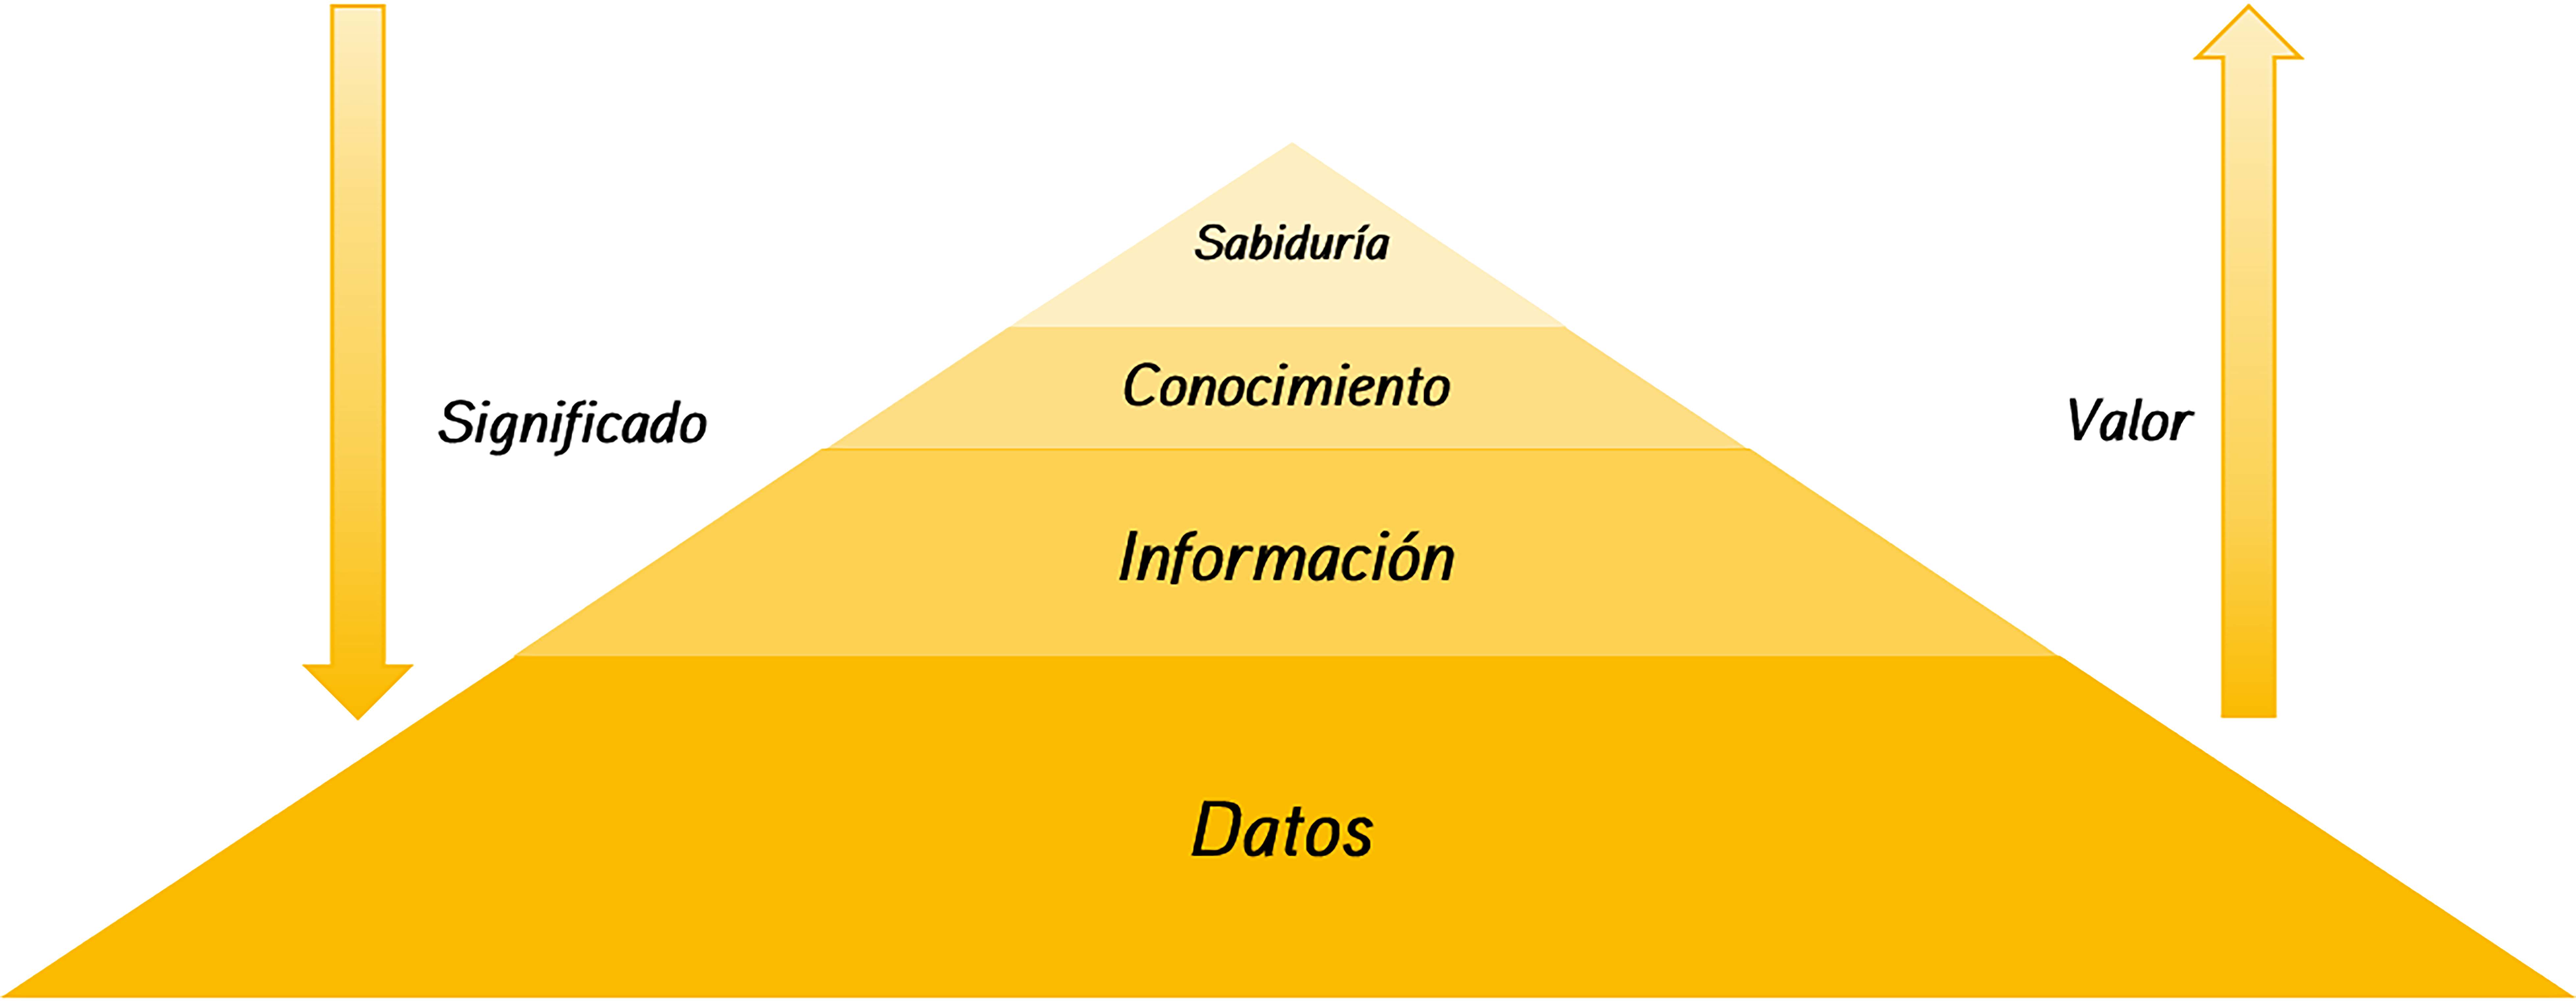
\includegraphics[width=0.8\textwidth,height=\textheight]{EDA/conocimiento.png}

}

\caption{\label{fig-cono}Jerarquía de Conocimiento}

\end{figure}

\begin{tcolorbox}[enhanced jigsaw, arc=.35mm, breakable, coltitle=black, left=2mm, opacityback=0, bottomtitle=1mm, colbacktitle=quarto-callout-tip-color!10!white, title=\textcolor{quarto-callout-tip-color}{\faLightbulb}\hspace{0.5em}{Claude Lévi-Strauss}, titlerule=0mm, colback=white, colframe=quarto-callout-tip-color-frame, bottomrule=.15mm, rightrule=.15mm, opacitybacktitle=0.6, toptitle=1mm, toprule=.15mm, leftrule=.75mm]

``El científico no es una persona que da las respuestas correctas, sino
una persona que hace las preguntas correctas.''

\end{tcolorbox}

\hypertarget{un-primer-vistazo-a-los-datos}{%
\section{Un primer vistazo a los
datos}\label{un-primer-vistazo-a-los-datos}}

En este tema vamos a trabajar con los datos de
\href{https://archive.ics.uci.edu/dataset/222/bank+marketing}{\textbf{Bank
Marketing}} del repositorio UCI. En primer lugar debemos comprender el
problema. ¿Qué sabes del marketing bancario? En el caso que nos ocupa,
los datos están relacionados con campañas de marketing directo (llamadas
telefónicas) de una entidad bancaria portuguesa. El objetivo de la
clasificación es \emph{predecir si el cliente suscribirá un depósito} a
plazo (variable objetivo).

Las variables que debemos estudiar son:

Variables de entrada:

\# datos del cliente bancario:

\begin{enumerate}
\def\labelenumi{\arabic{enumi}.}
\item
  edad (variable numérica)
\item
  empleo : tipo de empleo (variable categórica con las siguientes
  categorías: ``admin.'', ``desconocido'', ``desempleado'',
  ``directivo'', ``empleada del hogar'', ``empresario'', ``estudiante'',
  ``obrero'', ``autónomo'', ``jubilado'', ``técnico'', ``servicios'')
\item
  estado civil : estado civil (variable categórica con categorías:
  ``casado'', ``divorciado'', ``soltero''; nota: ``divorciado''
  significa divorciado o viudo)
\item
  educación (variable categórica con categorías: ``desconocida'',
  ``secundaria'', ``primaria'', ``terciaria'')
\item
  impago: ¿tiene un crédito impagado? (variable binaria con dos posibles
  valores: ``sí'', ``no'')
\item
  saldo: saldo medio anual, en euros (variable numérica)
\item
  vivienda: ¿tiene préstamo para vivienda? (variable binaria: ``sí'',
  ``no'')
\item
  préstamo: ¿tiene préstamo personal? (variable binaria: ``sí'', ``no'')

  \# relacionado con el último contacto de la campaña actual:
\item
  contacto: tipo de comunicación del contacto (variable categórica:
  ``desconocido'', ``teléfono'', ``móvil'')
\item
  día: día del mes del último contacto (variable numérica)
\item
  mes: mes del año del último contacto (variable categórica: ``ene'',
  ``feb'', ``mar'', \ldots, ``nov'', ``dic'')
\item
  duración: duración del último contacto, en segundos (variable
  numérica)
\end{enumerate}

\# otros atributos

\begin{enumerate}
\def\labelenumi{\arabic{enumi}.}
\setcounter{enumi}{12}
\item
  campaña: número de contactos realizados durante esta campaña y para
  este cliente (variable numérica, incluye el último contacto)
\item
  pdays: número de días transcurridos desde que el cliente fue
  contactado por última vez en una campaña anterior (variable numérica,
  -1 significa que el cliente no fue contactado previamente)
\item
  previous: número de contactos realizados antes de esta campaña y para
  este cliente (variable numérica)
\item
  poutcome: resultado de la campaña de marketing anterior (variable
  categórica: ``desconocido'', ``otro'', ``fracaso'', ``éxito'')
\end{enumerate}

\# Variable de salida (objetivo deseado):

17 - y: ¿ha suscrito el cliente un depósito a plazo? (variable binaria:
``sí'', ``no'')

\begin{tcolorbox}[enhanced jigsaw, arc=.35mm, breakable, coltitle=black, left=2mm, opacityback=0, bottomtitle=1mm, colbacktitle=quarto-callout-important-color!10!white, title=\textcolor{quarto-callout-important-color}{\faExclamation}\hspace{0.5em}{Para recordar}, titlerule=0mm, colback=white, colframe=quarto-callout-important-color-frame, bottomrule=.15mm, rightrule=.15mm, opacitybacktitle=0.6, toptitle=1mm, toprule=.15mm, leftrule=.75mm]

A veces (muchas veces) la descripción que encontramos en una primera
etapa no coincide al completo con los datos que luego nos entrega el
cliente.

En otras ocasiones no se dispone de la descripción de las variables. En
ese caso, ¡hay que hacer lo imposible por conseguirla!

\end{tcolorbox}

Leemos los datos con R.

\begin{Shaded}
\begin{Highlighting}[]
\FunctionTok{library}\NormalTok{(tidyverse)}
\NormalTok{bank }\OtherTok{=} \FunctionTok{read.csv}\NormalTok{(}\StringTok{\textquotesingle{}https://raw.githubusercontent.com/rafiag/DTI2020/main/data/bank.csv\textquotesingle{}}\NormalTok{)}
\FunctionTok{dim}\NormalTok{(bank)}
\end{Highlighting}
\end{Shaded}

\begin{verbatim}
[1] 11162    17
\end{verbatim}

\begin{Shaded}
\begin{Highlighting}[]
\NormalTok{bank}\OtherTok{=}\FunctionTok{as.tibble}\NormalTok{(bank)}
\NormalTok{bank}
\end{Highlighting}
\end{Shaded}

\begin{verbatim}
# A tibble: 11,162 x 17
     age job       marital education default balance housing loan  contact   day
   <int> <chr>     <chr>   <chr>     <chr>     <int> <chr>   <chr> <chr>   <int>
 1    59 admin.    married secondary no         2343 yes     no    unknown     5
 2    56 admin.    married secondary no           45 no      no    unknown     5
 3    41 technici~ married secondary no         1270 yes     no    unknown     5
 4    55 services  married secondary no         2476 yes     no    unknown     5
 5    54 admin.    married tertiary  no          184 no      no    unknown     5
 6    42 manageme~ single  tertiary  no            0 yes     yes   unknown     5
 7    56 manageme~ married tertiary  no          830 yes     yes   unknown     6
 8    60 retired   divorc~ secondary no          545 yes     no    unknown     6
 9    37 technici~ married secondary no            1 yes     no    unknown     6
10    28 services  single  secondary no         5090 yes     no    unknown     6
# i 11,152 more rows
# i 7 more variables: month <chr>, duration <int>, campaign <int>, pdays <int>,
#   previous <int>, poutcome <chr>, deposit <chr>
\end{verbatim}

Disponemos de más de 10000 observaciones y un total de 17 variables.

\hypertarget{tipo-de-variables-1}{%
\section{Tipo de variables}\label{tipo-de-variables-1}}

Para averiguar qué tipo de variables manejamos, ejecutar:

\begin{Shaded}
\begin{Highlighting}[]
\FunctionTok{str}\NormalTok{(bank)}
\end{Highlighting}
\end{Shaded}

\begin{verbatim}
tibble [11,162 x 17] (S3: tbl_df/tbl/data.frame)
 $ age      : int [1:11162] 59 56 41 55 54 42 56 60 37 28 ...
 $ job      : chr [1:11162] "admin." "admin." "technician" "services" ...
 $ marital  : chr [1:11162] "married" "married" "married" "married" ...
 $ education: chr [1:11162] "secondary" "secondary" "secondary" "secondary" ...
 $ default  : chr [1:11162] "no" "no" "no" "no" ...
 $ balance  : int [1:11162] 2343 45 1270 2476 184 0 830 545 1 5090 ...
 $ housing  : chr [1:11162] "yes" "no" "yes" "yes" ...
 $ loan     : chr [1:11162] "no" "no" "no" "no" ...
 $ contact  : chr [1:11162] "unknown" "unknown" "unknown" "unknown" ...
 $ day      : int [1:11162] 5 5 5 5 5 5 6 6 6 6 ...
 $ month    : chr [1:11162] "may" "may" "may" "may" ...
 $ duration : int [1:11162] 1042 1467 1389 579 673 562 1201 1030 608 1297 ...
 $ campaign : int [1:11162] 1 1 1 1 2 2 1 1 1 3 ...
 $ pdays    : int [1:11162] -1 -1 -1 -1 -1 -1 -1 -1 -1 -1 ...
 $ previous : int [1:11162] 0 0 0 0 0 0 0 0 0 0 ...
 $ poutcome : chr [1:11162] "unknown" "unknown" "unknown" "unknown" ...
 $ deposit  : chr [1:11162] "yes" "yes" "yes" "yes" ...
\end{verbatim}

Creamos las particiones sobre los datos y trabajamos sobre la partición
de entrenamiento.

\begin{Shaded}
\begin{Highlighting}[]
\CommentTok{\# Parciticionamos los datos}
\FunctionTok{set.seed}\NormalTok{(}\DecValTok{2138}\NormalTok{)}
\NormalTok{n}\OtherTok{=}\FunctionTok{dim}\NormalTok{(bank)[}\DecValTok{1}\NormalTok{]}
\NormalTok{indices}\OtherTok{=}\FunctionTok{seq}\NormalTok{(}\DecValTok{1}\SpecialCharTok{:}\NormalTok{n)}
\NormalTok{indices.train}\OtherTok{=}\FunctionTok{sample}\NormalTok{(indices,}\AttributeTok{size=}\NormalTok{n}\SpecialCharTok{*}\NormalTok{.}\DecValTok{5}\NormalTok{,}\AttributeTok{replace=}\ConstantTok{FALSE}\NormalTok{)}
\NormalTok{indices.test}\OtherTok{=}\FunctionTok{sample}\NormalTok{(indices[}\SpecialCharTok{{-}}\NormalTok{indices.train],}\AttributeTok{size=}\NormalTok{n}\SpecialCharTok{*}\NormalTok{.}\DecValTok{25}\NormalTok{,}\AttributeTok{replace=}\ConstantTok{FALSE}\NormalTok{)}
\NormalTok{indices.valid}\OtherTok{=}\NormalTok{indices[}\SpecialCharTok{{-}}\FunctionTok{c}\NormalTok{(indices.train,indices.test)]}

\NormalTok{bank.train}\OtherTok{=}\NormalTok{bank[indices.train,]}
\NormalTok{bank.test}\OtherTok{=}\NormalTok{bank[indices.test,]}
\NormalTok{bank.valid}\OtherTok{=}\NormalTok{bank[indices.valid,]}
\end{Highlighting}
\end{Shaded}

\begin{tcolorbox}[enhanced jigsaw, arc=.35mm, breakable, coltitle=black, left=2mm, opacityback=0, bottomtitle=1mm, colbacktitle=quarto-callout-caution-color!10!white, title=\textcolor{quarto-callout-caution-color}{\faFire}\hspace{0.5em}{Atrévete}, titlerule=0mm, colback=white, colframe=quarto-callout-caution-color-frame, bottomrule=.15mm, rightrule=.15mm, opacitybacktitle=0.6, toptitle=1mm, toprule=.15mm, leftrule=.75mm]

¿Te has hecho (ya) alguna pregunta sobre los datos? Si es así, no
esperes más, busca la respuesta!

\end{tcolorbox}

Por ejemplo, ¿qué te parecen estas preguntas que nosotros proponemos?

¿Qué día del año se producen más depósitos por parte de los estudiantes?

\begin{Shaded}
\begin{Highlighting}[]
\NormalTok{bank.train }\SpecialCharTok{\%\textgreater{}\%} 
  \FunctionTok{filter}\NormalTok{(deposit}\SpecialCharTok{==}\StringTok{"yes"}\NormalTok{) }\SpecialCharTok{\%\textgreater{}\%} 
  \FunctionTok{count}\NormalTok{(month, day) }\SpecialCharTok{\%\textgreater{}\%} 
  \FunctionTok{top\_n}\NormalTok{(}\DecValTok{1}\NormalTok{,n)}
\end{Highlighting}
\end{Shaded}

\begin{verbatim}
# A tibble: 1 x 3
  month   day     n
  <chr> <int> <int>
1 apr      30    79
\end{verbatim}

¿En qué mes del año realizan más depósitos los estudiantes?

\begin{Shaded}
\begin{Highlighting}[]
\NormalTok{bank.train }\SpecialCharTok{\%\textgreater{}\%} 
  \FunctionTok{filter}\NormalTok{(deposit}\SpecialCharTok{==}\StringTok{"yes"} \SpecialCharTok{\&}\NormalTok{ job}\SpecialCharTok{==}\StringTok{"student"}\NormalTok{) }\SpecialCharTok{\%\textgreater{}\%} 
  \FunctionTok{count}\NormalTok{(month) }\SpecialCharTok{\%\textgreater{}\%} 
  \FunctionTok{top\_n}\NormalTok{(}\DecValTok{1}\NormalTok{,n)}
\end{Highlighting}
\end{Shaded}

\begin{verbatim}
# A tibble: 1 x 2
  month     n
  <chr> <int>
1 apr      21
\end{verbatim}

¿Qué trabajo está asociado con el mayor porcentaje de depósitos?

\begin{Shaded}
\begin{Highlighting}[]
\NormalTok{bank.train }\SpecialCharTok{\%\textgreater{}\%}
  \FunctionTok{group\_by}\NormalTok{(job) }\SpecialCharTok{\%\textgreater{}\%}
  \FunctionTok{mutate}\NormalTok{(}\AttributeTok{d =} \FunctionTok{n}\NormalTok{()) }\SpecialCharTok{\%\textgreater{}\%}
  \FunctionTok{group\_by}\NormalTok{(job, deposit) }\SpecialCharTok{\%\textgreater{}\%}
  \FunctionTok{summarise}\NormalTok{(}\AttributeTok{Perc =} \FunctionTok{n}\NormalTok{()}\SpecialCharTok{/}\FunctionTok{first}\NormalTok{(d), }\AttributeTok{.groups =} \StringTok{"drop"}\NormalTok{) }\SpecialCharTok{\%\textgreater{}\%}
  \FunctionTok{pivot\_wider}\NormalTok{(}
    \AttributeTok{id\_cols =}\NormalTok{ job,}
    \AttributeTok{names\_from =}\NormalTok{ deposit,}
    \AttributeTok{values\_from =}\NormalTok{ Perc}
\NormalTok{  ) }\SpecialCharTok{\%\textgreater{}\%}
  \FunctionTok{top\_n}\NormalTok{(}\DecValTok{1}\NormalTok{)}
\end{Highlighting}
\end{Shaded}

\begin{verbatim}
# A tibble: 1 x 3
  job        no   yes
  <chr>   <dbl> <dbl>
1 student 0.218 0.782
\end{verbatim}

\begin{tcolorbox}[enhanced jigsaw, arc=.35mm, breakable, coltitle=black, left=2mm, opacityback=0, bottomtitle=1mm, colbacktitle=quarto-callout-caution-color!10!white, title=\textcolor{quarto-callout-caution-color}{\faFire}\hspace{0.5em}{Repaso}, titlerule=0mm, colback=white, colframe=quarto-callout-caution-color-frame, bottomrule=.15mm, rightrule=.15mm, opacitybacktitle=0.6, toptitle=1mm, toprule=.15mm, leftrule=.75mm]

\texttt{dplyr} es un paquete en R diseñado para facilitar la
manipulación y transformación de datos de manera eficiente y
estructurada. Fue desarrollado por \textbf{Hadley Wickham} y se ha
convertido en una de las herramientas más populares en la ciencia de
datos y análisis de datos.

\end{tcolorbox}

\hypertarget{variable-objetivo}{%
\section{Variable objetivo}\label{variable-objetivo}}

En el ámbito del Aprendizaje Automático, en problemas de clasificación
(Aprendizaje Supervisado) existe una variable de interés fundamental, es
la variable respuesta o variable objetivo. En el caso que nos ocupa
dicha variable es la característica: ``deposit''. Vamos a estudiar la
información que nos proporciona dicha variable.

\begin{Shaded}
\begin{Highlighting}[]
\FunctionTok{library}\NormalTok{(ggplot2)}
\FunctionTok{table}\NormalTok{(bank.train}\SpecialCharTok{$}\NormalTok{deposit)}
\end{Highlighting}
\end{Shaded}

\begin{verbatim}

  no  yes 
2908 2673 
\end{verbatim}

\begin{Shaded}
\begin{Highlighting}[]
\FunctionTok{ggplot}\NormalTok{(}\AttributeTok{data=}\NormalTok{bank.train,}\FunctionTok{aes}\NormalTok{(}\AttributeTok{x=}\NormalTok{deposit,}\AttributeTok{fill=}\NormalTok{deposit)) }\SpecialCharTok{+}
  \FunctionTok{geom\_bar}\NormalTok{(}\FunctionTok{aes}\NormalTok{(}\AttributeTok{y=}\NormalTok{(..count..)}\SpecialCharTok{/}\FunctionTok{sum}\NormalTok{(..count..))) }\SpecialCharTok{+}
  \FunctionTok{scale\_y\_continuous}\NormalTok{(}\AttributeTok{labels=}\NormalTok{scales}\SpecialCharTok{::}\NormalTok{percent) }\SpecialCharTok{+}
  \FunctionTok{theme}\NormalTok{(}\AttributeTok{legend.position=}\StringTok{"none"}\NormalTok{) }\SpecialCharTok{+}
  \FunctionTok{ylab}\NormalTok{(}\StringTok{"Frecuencia relativa"}\NormalTok{) }\SpecialCharTok{+}
  \FunctionTok{xlab}\NormalTok{(}\StringTok{"Variable respuesta: deposit"}\NormalTok{)}
\end{Highlighting}
\end{Shaded}

\begin{figure}[H]

{\centering 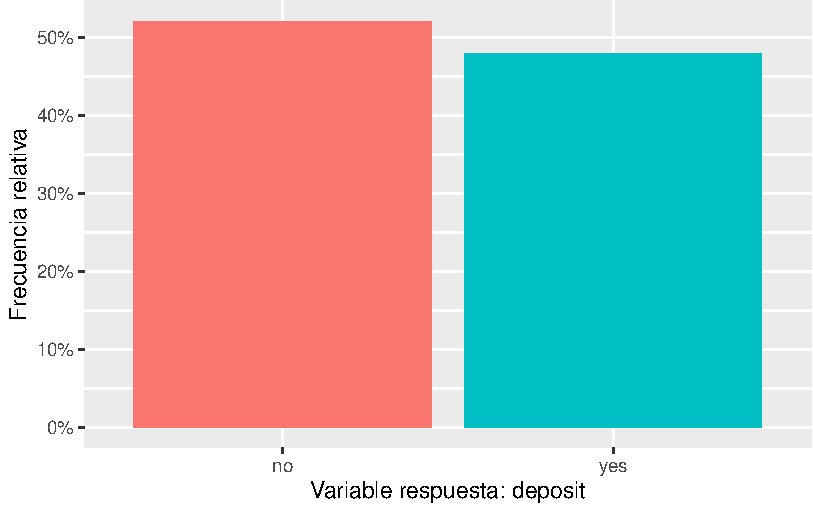
\includegraphics{eda_files/figure-pdf/variable_objetivo-1.pdf}

}

\end{figure}

\hypertarget{visualizar-distribuciones}{%
\section{Visualizar distribuciones}\label{visualizar-distribuciones}}

La forma de visualizar la distribución de una variable dependerá de si
la variable es categórica o continua. Una variable es categórica si sólo
puede tomar uno de un pequeño conjunto de valores. En R, las variables
categóricas suelen guardarse como factores o vectores de caracteres.
Para examinar la distribución de una variable categórica, utiliza un
gráfico de barras:

\begin{Shaded}
\begin{Highlighting}[]
\FunctionTok{ggplot}\NormalTok{(}\AttributeTok{data =}\NormalTok{ bank.train) }\SpecialCharTok{+}
  \FunctionTok{geom\_bar}\NormalTok{(}\AttributeTok{mapping =} \FunctionTok{aes}\NormalTok{(}\AttributeTok{x =}\NormalTok{ contact))}
\end{Highlighting}
\end{Shaded}

\begin{figure}[H]

{\centering 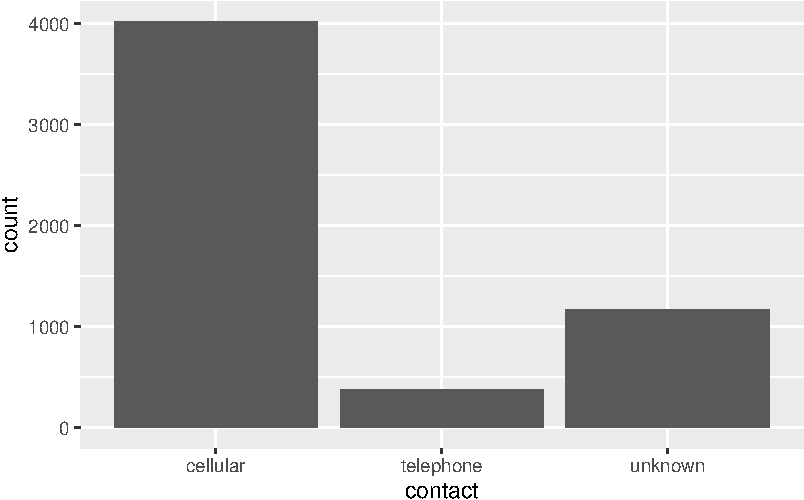
\includegraphics{eda_files/figure-pdf/unnamed-chunk-8-1.pdf}

}

\end{figure}

Puedes obtener los valores exactos en cada categoría como sigue:

\begin{Shaded}
\begin{Highlighting}[]
\NormalTok{bank.train}\SpecialCharTok{\%\textgreater{}\%} 
  \FunctionTok{count}\NormalTok{(contact)}
\end{Highlighting}
\end{Shaded}

\begin{verbatim}
# A tibble: 3 x 2
  contact       n
  <chr>     <int>
1 cellular   4025
2 telephone   383
3 unknown    1173
\end{verbatim}

Una variable es continua si puede tomar cualquiera de un conjunto
infinito de valores ordenados. Para examinar la distribución de una
variable continua, utiliza un histograma:

\begin{Shaded}
\begin{Highlighting}[]
\FunctionTok{ggplot}\NormalTok{(}\AttributeTok{data =}\NormalTok{ bank.train) }\SpecialCharTok{+}
  \FunctionTok{geom\_histogram}\NormalTok{(}\AttributeTok{mapping =} \FunctionTok{aes}\NormalTok{(}\AttributeTok{x =}\NormalTok{ age), }\AttributeTok{binwidth =} \DecValTok{5}\NormalTok{)}
\end{Highlighting}
\end{Shaded}

\begin{figure}[H]

{\centering 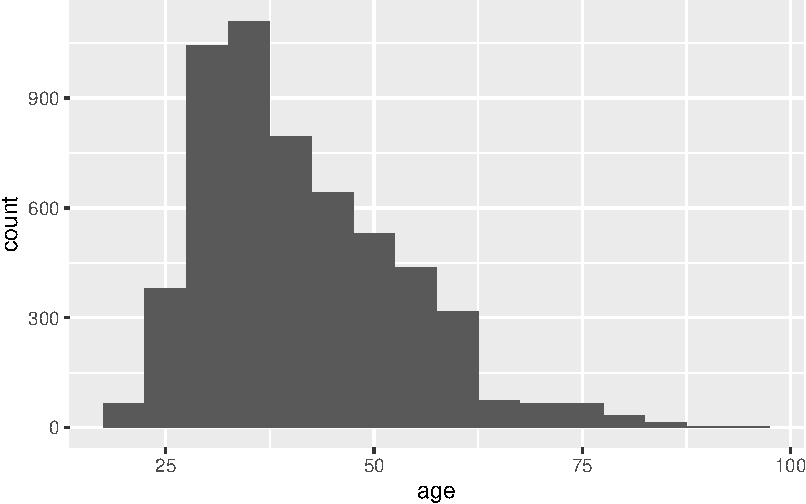
\includegraphics{eda_files/figure-pdf/unnamed-chunk-10-1.pdf}

}

\end{figure}

Un histograma divide el eje \(x\) en intervalos equidistantes y, a
continuación, utiliza la altura de una barra para mostrar el número de
observaciones que se encuentran en cada intervalo. En el gráfico
anterior, la primera barra muestra unas 100 observaciones (realmente son
119) tienen un valor de edad por debajo de 22.5 años. Puede establecer
la anchura de los intervalos en un histograma con el argumento binwidth,
que se mide en las unidades de la variable \(x\).

\begin{tcolorbox}[enhanced jigsaw, arc=.35mm, breakable, coltitle=black, left=2mm, opacityback=0, bottomtitle=1mm, colbacktitle=quarto-callout-important-color!10!white, title=\textcolor{quarto-callout-important-color}{\faExclamation}\hspace{0.5em}{Para recordar}, titlerule=0mm, colback=white, colframe=quarto-callout-important-color-frame, bottomrule=.15mm, rightrule=.15mm, opacitybacktitle=0.6, toptitle=1mm, toprule=.15mm, leftrule=.75mm]

Siempre se deben explorar una variedad de anchos de intervalo cuando
trabajamos con histogramas, ya que diferentes anchos de intervalo pueden
revelar diferentes patrones.

\end{tcolorbox}

Podemos representar funciones de densidad de probabilidad.

\begin{Shaded}
\begin{Highlighting}[]
\FunctionTok{ggplot}\NormalTok{(bank.train, }\FunctionTok{aes}\NormalTok{(}\AttributeTok{x =}\NormalTok{ age)) }\SpecialCharTok{+}
\FunctionTok{geom\_density}\NormalTok{() }\SpecialCharTok{+}
\FunctionTok{ggtitle}\NormalTok{(}\StringTok{\textquotesingle{}KDE de edad en datos bank\textquotesingle{}}\NormalTok{)}
\end{Highlighting}
\end{Shaded}

\begin{figure}[H]

{\centering 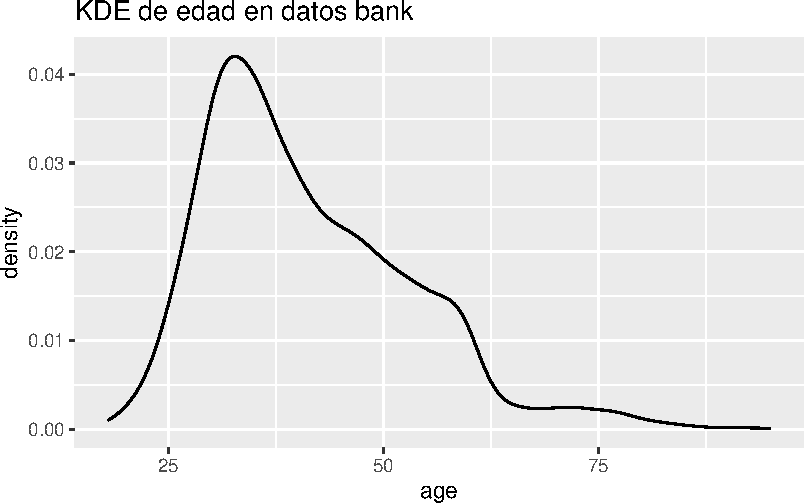
\includegraphics{eda_files/figure-pdf/unnamed-chunk-11-1.pdf}

}

\end{figure}

Otro gráfico muy utilizado para variables cuantitativas univariantes es
el \emph{boxplot}, también llamado \emph{box-and-whisker plot} (diagrama
de caja y bigotes). Es especialmente útil para detectar posibles datos
atípicos en los valores de una variable, siempre que su distribución sea
parecida a una distribución \emph{Normal}. El gráfico muestra:

\begin{itemize}
\item
  Una caja cuyos límites son el primer y el tercel cuartil de la
  distribución de valores.
\item
  Una línea central, que marca la mediana.
\item
  Los bigotes, que por defecto (en R) se extienden hasta 1.5 veces el
  valor del rango intercuartílico (IQR) por encima y por debajo de la
  caja.
\item
  Puntos individuales, que quedan más allá del límite de los bigotes,
  marcan posibles datos atípicos.
\end{itemize}

En distribuciones muy asimétricas o con muchos valores extremos, muy
diferentes a una distribución \emph{Normal}, aparecerán demasiados
puntos más allá de los bigotes y no se podrán apreciar fácilmente los
atípicos (demasiados puntos considerados como tales). En ese caso, es
conveniente intentar una transformación de la variable antes de
representar el \emph{boxplot}.

\begin{Shaded}
\begin{Highlighting}[]
\FunctionTok{ggplot}\NormalTok{(bank.train, }\FunctionTok{aes}\NormalTok{(}\AttributeTok{x=}\NormalTok{deposit, }\AttributeTok{y=}\NormalTok{age, }\AttributeTok{color=}\NormalTok{deposit)) }\SpecialCharTok{+}
  \FunctionTok{geom\_boxplot}\NormalTok{()}
\end{Highlighting}
\end{Shaded}

\begin{figure}[H]

{\centering 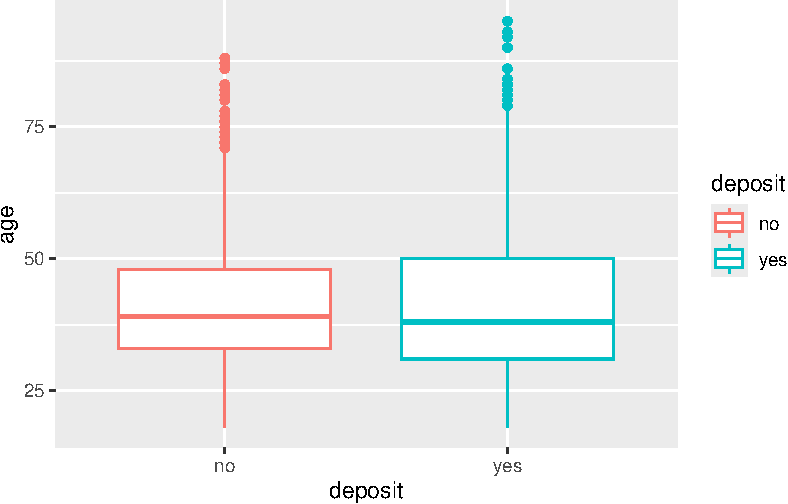
\includegraphics{eda_files/figure-pdf/unnamed-chunk-12-1.pdf}

}

\end{figure}

\hypertarget{transformaciuxf3n-de-variables}{%
\section{Transformación de
variables}\label{transformaciuxf3n-de-variables}}

\hypertarget{transformaciuxf3n-de-variables-cuantitativas}{%
\subsection{Transformación de variables
cuantitativas}\label{transformaciuxf3n-de-variables-cuantitativas}}

En algunos métodos de ML es necesario contar con variables que cumplan
requisitos de normalidad. Por ejemplo, si tomamos la transformación
\(log\) sobre la variable \texttt{edad} obtenemos una distribución
multimodal que, probablemente, corresponda a la combinación de dos (o
más) normales.

\begin{Shaded}
\begin{Highlighting}[]
\FunctionTok{ggplot}\NormalTok{(}\AttributeTok{data =}\NormalTok{ bank.train) }\SpecialCharTok{+}
  \FunctionTok{geom\_histogram}\NormalTok{(}\AttributeTok{mapping =} \FunctionTok{aes}\NormalTok{(}\AttributeTok{x =} \FunctionTok{log}\NormalTok{(age)), }\AttributeTok{binwidth =}\NormalTok{ .}\DecValTok{1}\NormalTok{)}
\end{Highlighting}
\end{Shaded}

\begin{figure}[H]

{\centering 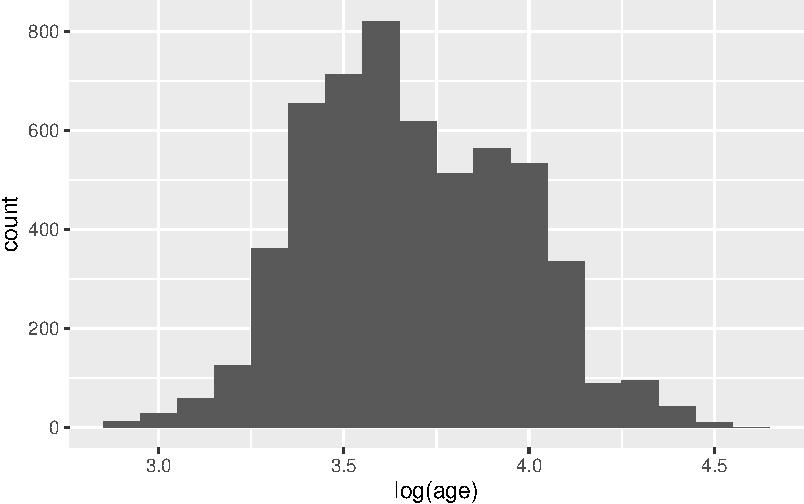
\includegraphics{eda_files/figure-pdf/unnamed-chunk-13-1.pdf}

}

\end{figure}

\begin{tcolorbox}[enhanced jigsaw, arc=.35mm, breakable, coltitle=black, left=2mm, opacityback=0, bottomtitle=1mm, colbacktitle=quarto-callout-important-color!10!white, title=\textcolor{quarto-callout-important-color}{\faExclamation}\hspace{0.5em}{Para recordar}, titlerule=0mm, colback=white, colframe=quarto-callout-important-color-frame, bottomrule=.15mm, rightrule=.15mm, opacitybacktitle=0.6, toptitle=1mm, toprule=.15mm, leftrule=.75mm]

Los modelos de ML serán tan buenos como lo sean las variables de entrada
de dichos algoritmos.

\end{tcolorbox}

\hypertarget{transformaciones-para-igualar-dispersiuxf3n}{%
\subsubsection{Transformaciones para igualar
dispersión}\label{transformaciones-para-igualar-dispersiuxf3n}}

Con frecuencia, el objetivo de la transformación de variables
cuantitativas es obtener una variable cuya distribución de valores sea:

\begin{itemize}
\item
  Más simétrica y con menor dispersión que la original.
\item
  Más semejante a una distribución normal (e.g.~para algunos modelos
  lineales).
\item
  Restringida en un intervalo de valores (e.g.~\([0,1]\) ).
\end{itemize}

La forma más sencilla de detectar que alguna de nuestras variables
necesita ser transformada es representar un gráfico que muestre la
distribución de valores de la variable. Por ejemplo, un histograma o un
diagrama de densidad de probabilidad (o ambos).

El uso de los logaritmos tiene su propia recomendación en preparación de
datos (Fox and Weisberg 2018):

\begin{tcolorbox}[enhanced jigsaw, arc=.35mm, breakable, coltitle=black, left=2mm, opacityback=0, bottomtitle=1mm, colbacktitle=quarto-callout-tip-color!10!white, title=\textcolor{quarto-callout-tip-color}{\faLightbulb}\hspace{0.5em}{John Fox}, titlerule=0mm, colback=white, colframe=quarto-callout-tip-color-frame, bottomrule=.15mm, rightrule=.15mm, opacitybacktitle=0.6, toptitle=1mm, toprule=.15mm, leftrule=.75mm]

``Si la variable es estrictamente positiva, no tiene un límite superior
para sus valores, y su rango abarca dos o más órdenes de magnitud
(potencias de 10), entonces la transformación logarítmica suele ser
útil. A la inversa, cuando la variable tiene un rango de valores pequeño
(menor de un orden de magnitud), el logaritmo o cualquier otra
transformación simple no ayudará mucho.''

\end{tcolorbox}

La versión general de esta transformación son las transformaciones de
escala-potencia (scaled-power transformations), también denominadas
transformaciones de \textbf{Box-Cox}.

\[x(\lambda)= \begin{cases} \frac{x^\lambda-1}{\lambda},& \text{cuando } \lambda \neq 0,\\ log_e(x), & \text{cuando } \lambda = 0 \end{cases}\]

La función \texttt{car::symbox(...)} permite probar varias combinaciones
típicas del parámetro λ , para comprobar con cuál de ellas obtenemos una
distribución más simétrica de valores.

\begin{Shaded}
\begin{Highlighting}[]
\FunctionTok{library}\NormalTok{(car)}

\NormalTok{bank.train }\SpecialCharTok{\%\textgreater{}\%} \FunctionTok{symbox}\NormalTok{(}\SpecialCharTok{\textasciitilde{}}\NormalTok{ age, }\AttributeTok{data =}\NormalTok{ .)}
\end{Highlighting}
\end{Shaded}

\begin{figure}[H]

{\centering 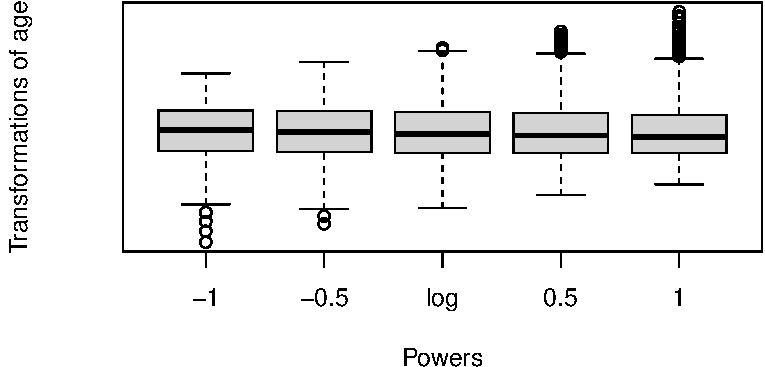
\includegraphics{eda_files/figure-pdf/unnamed-chunk-14-1.pdf}

}

\end{figure}

\hypertarget{transformaciones-para-igualar-dispersiuxf3n-1}{%
\subsubsection{Transformaciones para igualar
dispersión}\label{transformaciones-para-igualar-dispersiuxf3n-1}}

También es bastante común aplicar transformaciones en datos
cuantitativos para igualar las escalas de representación de las
variables. En muchos modelos, si una de nuestras variables tiene una
escala mucho mayor que las demás, sus valores tienden a predominar en
los resultados, enmascarando la influencia del resto de variables en el
modelo.

Por este motivo, en muchos modelos es importante garantizar que todas
las variables se representan en escalas comparables, de forma que
ninguna predomine sobre el resto. Conviene aclarar un poco algunos
términos que se suelen emplear de forma indistinta:

\begin{itemize}
\item
  \textbf{Reescalado o cambio de escala}: Consiste en sumar o restar una
  constante a un vector, y luego multiplicar o dividir por una
  constante. Por ejemplo, para transformar la unidad de medida de una
  variable (grados Farenheit → grados Celsius).
\item
  \textbf{Normalización}: Consiste en dividir por la norma de un vector,
  por ejemplo para hacer su distancia euclídea igual a \(1\).
\item
  \textbf{Estandarización}: Consiste en restar a un vector una medida de
  localización o nivel (e.g.~media, mediana) y dividir por una medida de
  escala (dispersión). Por ejemplo, si restamos la media y dividimos por
  la desviación típica hacemos que la distribución tenga media \(0\) y
  desviación típica \(1\).
\end{itemize}

Algunas aternativas comunes son:

\[
Estandarización \rightarrow Y=\frac{X-\overline{x}}{s_x}
\]

\[
Escalado \space min-max \rightarrow Y=\frac{X-min_x}{max_x-min_x}
\]

En R, la función \texttt{scale()} se puede utilizar para realizar estas
operaciones de estandarización. Automáticamente, puede actuar sobre las
columnas de un \texttt{data.frame}, aplicando la misma operación a todas
ellas (siempre que todas sean cuantitativas).

\hypertarget{transformaciuxf3n-de-variables-cualitativas}{%
\subsection{Transformación de variables
cualitativas}\label{transformaciuxf3n-de-variables-cualitativas}}

A diferencia de las variables cuantitativas, que representan cantidades
numéricas, las variables cualitativas, también conocidas como variables
categóricas, se utilizan para describir características o cualidades que
no tienen un valor numérico intrínseco. Las variables cualitativas son
esenciales en la investigación y el análisis de datos, ya que a menudo
se utilizan para clasificar, segmentar y comprender información sobre
grupos, categorías o características. Algunas técnicas comunes para
analizar variables cualitativas incluyen la creación de tablas de
frecuencia para contar la ocurrencia de cada categoría y el uso de
gráficos como gráficos de barras o diagramas de sectores para visualizar
la distribución de categorías. Estos análisis pueden proporcionar
información valiosa sobre patrones, tendencias y relaciones en los datos
cualitativos, lo que puede ser fundamental para tomar decisiones
informadas en una amplia gama de campos, desde marketing hasta
investigación social y más.

Las variables cualitativas se dividen en dos categorías principales:

\begin{tcolorbox}[enhanced jigsaw, arc=.35mm, breakable, coltitle=black, left=2mm, opacityback=0, bottomtitle=1mm, colbacktitle=quarto-callout-note-color!10!white, title=\textcolor{quarto-callout-note-color}{\faInfo}\hspace{0.5em}{Variables Cualitativas Nominales}, titlerule=0mm, colback=white, colframe=quarto-callout-note-color-frame, bottomrule=.15mm, rightrule=.15mm, opacitybacktitle=0.6, toptitle=1mm, toprule=.15mm, leftrule=.75mm]

Las variables nominales representan categorías o etiquetas que no tienen
un orden inherente. Ejemplos comunes incluyen el género (masculino,
femenino, otro), el estado civil (soltero, casado, divorciado) o los
colores (rojo, azul, verde). No se pueden realizar operaciones
matemáticas en variables nominales, como sumar o restar.

\end{tcolorbox}

\begin{tcolorbox}[enhanced jigsaw, arc=.35mm, breakable, coltitle=black, left=2mm, opacityback=0, bottomtitle=1mm, colbacktitle=quarto-callout-note-color!10!white, title=\textcolor{quarto-callout-note-color}{\faInfo}\hspace{0.5em}{Variables Cualitativas Ordinales}, titlerule=0mm, colback=white, colframe=quarto-callout-note-color-frame, bottomrule=.15mm, rightrule=.15mm, opacitybacktitle=0.6, toptitle=1mm, toprule=.15mm, leftrule=.75mm]

Las variables ordinales representan categorías con un orden natural o
jerarquía, pero la distancia entre las categorías no es necesariamente
uniforme ni conocida. Ejemplos incluyen la calificación de satisfacción
del cliente (muy insatisfecho, insatisfecho, neutral, satisfecho, muy
satisfecho) o el nivel de educación (primaria, secundaria,
universitaria). Aunque se pueden establecer comparaciones de orden (por
ejemplo, ``mayor que'' o ``menor que''), no es apropiado realizar
operaciones matemáticas en variables ordinales.

\end{tcolorbox}

En R, las variables categóricas se denominan \textbf{factores} (factors)
y sus categorías \textbf{niveles} (levels). Es importante procesarlos
adecuadamente para que los modelos aprovechen la información que
contienen estas variables. Por otro lado, si se codifica incorrectamente
esta información los modelos pueden estar realizando operaciones
absurdas aunque nos devuelvan resultados aparentemente válidos.

\begin{tcolorbox}[enhanced jigsaw, arc=.35mm, breakable, coltitle=black, left=2mm, opacityback=0, bottomtitle=1mm, colbacktitle=quarto-callout-warning-color!10!white, title=\textcolor{quarto-callout-warning-color}{\faExclamationTriangle}\hspace{0.5em}{R}, titlerule=0mm, colback=white, colframe=quarto-callout-warning-color-frame, bottomrule=.15mm, rightrule=.15mm, opacitybacktitle=0.6, toptitle=1mm, toprule=.15mm, leftrule=.75mm]

Por defecto, R transforma columnas tipo string en factores al leer los
datos de un archivo. Además, por defecto, R \textbf{ordena los niveles
de los factores alfabéticamente}, según sus etiquetas. Debemos tener
cuidado con esto, puesto que en muchos análisis es muy importante saber
qué nivel se está tomando como referencia, de entre los valores posibles
de un factor, para comparar con los restantes. En ciertos modelos, la
elección como referencia de uno de los valores del factor (típicamente
el primero que aparece en la lista de niveles) cambia por completo los
resultados, así como la interpretación de los mismos.

\end{tcolorbox}

En variables ordinales se debe respetar estrictamente el orden
preestablecido de los niveles. Por ejemplo, una ordenación (``regular''
\textless{} ``bueno'' \textless{} ``malo'') es inaceptable. Para
establecer una ordenación explícita entre los niveles hay que
especificarla manualmente si no coincide con la alfabética, y además
configurar el argumento ordered = TRUE en la función factor():

\begin{Shaded}
\begin{Highlighting}[]
\NormalTok{satisfaccion }\OtherTok{\textless{}{-}} \FunctionTok{rep}\NormalTok{(}\FunctionTok{c}\NormalTok{(}\StringTok{"malo"}\NormalTok{, }\StringTok{"bueno"}\NormalTok{, }\StringTok{"regular"}\NormalTok{), }\FunctionTok{c}\NormalTok{(}\DecValTok{3}\NormalTok{,}\DecValTok{3}\NormalTok{,}\DecValTok{3}\NormalTok{))}
\NormalTok{satisfaccion }\OtherTok{\textless{}{-}} \FunctionTok{factor}\NormalTok{(satisfaccion, }\AttributeTok{ordered =} \ConstantTok{TRUE}\NormalTok{, }\AttributeTok{levels =} \FunctionTok{c}\NormalTok{(}\StringTok{"malo"}\NormalTok{, }\StringTok{"regular"}\NormalTok{, }\StringTok{"bueno"}\NormalTok{))}
\NormalTok{satisfaccion}
\end{Highlighting}
\end{Shaded}

\begin{verbatim}
[1] malo    malo    malo    bueno   bueno   bueno   regular regular regular
Levels: malo < regular < bueno
\end{verbatim}

Para comprobar qué nivel se toma como referencia en cada uno de los
factores de una base de datos usamos la funión \texttt{levels()}:

\begin{Shaded}
\begin{Highlighting}[]
\FunctionTok{levels}\NormalTok{(bank.train}\SpecialCharTok{$}\NormalTok{marital)}
\end{Highlighting}
\end{Shaded}

\begin{verbatim}
NULL
\end{verbatim}

Y esto, ¿es correcto? Veamos la distribución de las observaciones en las
categorías de la variable \texttt{marital}:

\begin{Shaded}
\begin{Highlighting}[]
\FunctionTok{ggplot}\NormalTok{(}\AttributeTok{data =}\NormalTok{ bank.train) }\SpecialCharTok{+}
  \FunctionTok{geom\_bar}\NormalTok{(}\AttributeTok{mapping =} \FunctionTok{aes}\NormalTok{(}\AttributeTok{x =}\NormalTok{ marital))}
\end{Highlighting}
\end{Shaded}

\begin{figure}[H]

{\centering 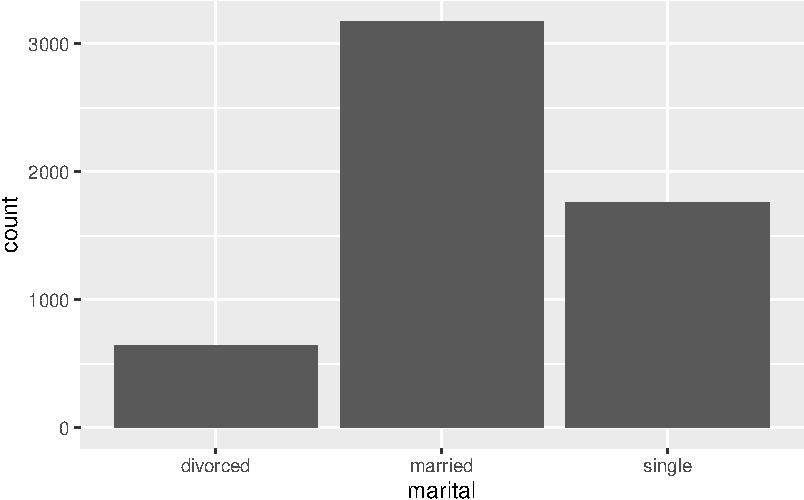
\includegraphics{eda_files/figure-pdf/unnamed-chunk-17-1.pdf}

}

\end{figure}

\begin{tcolorbox}[enhanced jigsaw, arc=.35mm, breakable, coltitle=black, left=2mm, opacityback=0, bottomtitle=1mm, colbacktitle=quarto-callout-warning-color!10!white, title=\textcolor{quarto-callout-warning-color}{\faExclamationTriangle}\hspace{0.5em}{Recomendación}, titlerule=0mm, colback=white, colframe=quarto-callout-warning-color-frame, bottomrule=.15mm, rightrule=.15mm, opacitybacktitle=0.6, toptitle=1mm, toprule=.15mm, leftrule=.75mm]

Habitualmente será más recomendable elegir como categoría de referencia
para variables categóricas aquella categoría con mayor número de
observaciones.

\end{tcolorbox}

Por tanto, en este caso particular deberíamos modificar la categoría de
referencia como sigue:

\begin{Shaded}
\begin{Highlighting}[]
\NormalTok{reorder\_marital }\OtherTok{=} \FunctionTok{factor}\NormalTok{(bank.train}\SpecialCharTok{$}\NormalTok{marital, }\AttributeTok{levels=}\NormalTok{(}\FunctionTok{c}\NormalTok{(}\StringTok{\textquotesingle{} married\textquotesingle{}}\NormalTok{, }\StringTok{\textquotesingle{} single\textquotesingle{}}\NormalTok{, }\StringTok{\textquotesingle{} divorced\textquotesingle{}}\NormalTok{)))}
\FunctionTok{levels}\NormalTok{(reorder\_marital)}
\end{Highlighting}
\end{Shaded}

\begin{verbatim}
[1] " married"  " single"   " divorced"
\end{verbatim}

Nótese que la nueva variable aquí creada, \texttt{reorder\_marital}, no
ha sido incluida (aún) en el tibble \texttt{bank}. Para ello:

\begin{Shaded}
\begin{Highlighting}[]
\NormalTok{bank.train}\SpecialCharTok{$}\NormalTok{marital }\OtherTok{=}\NormalTok{ reorder\_marital}
\end{Highlighting}
\end{Shaded}

\hypertarget{conversiuxf3n-de-variables-cuantitativas-a-variables-categuxf3ricas}{%
\subsubsection{Conversión de variables cuantitativas a variables
categóricas}\label{conversiuxf3n-de-variables-cuantitativas-a-variables-categuxf3ricas}}

La conversión de variables cuantitativas a variables categóricas es un
proceso importante en EDA que implica transformar datos numéricos en
categorías. Esto se realiza con el propósito de simplificar el análisis,
resaltar patrones específicos y facilitar la interpretación de los
resultados. A continuación, se destacan algunas situaciones comunes en
las que se realiza esta conversión y cómo se lleva a cabo:

\begin{enumerate}
\def\labelenumi{\arabic{enumi}.}
\item
  \textbf{Agrupación de datos numéricos:} En ocasiones, es útil agrupar
  datos numéricos en intervalos o categorías para resaltar tendencias
  generales. Por ejemplo, en un estudio de edades de una población, en
  lugar de analizar cada edad individual, se pueden crear grupos como
  ``menos de 18 años'', ``18-30 años'', ``31-45 años'' y así
  sucesivamente.
\item
  \textbf{Creación de variables binarias:} A menudo, se convierten
  variables numéricas en variables binarias (\(1\) o \(0\)) para
  simplificar el análisis. Por ejemplo, en un estudio de satisfacción
  del cliente, se puede crear una variable binaria donde ``\(1\)''
  indica clientes satisfechos y ``\(0\)'' indica clientes insatisfechos.
\item
  \textbf{Categorización de variables continuas:} Las variables
  continuas, como ingresos o puntuaciones, se pueden convertir en
  categorías para segmentar la población. Esto puede ser útil en
  análisis demográficos o de segmentación de mercado.
\item
  \textbf{Simplificación de modelos:} Algunos modelos de ML pueden
  beneficiarse de la conversión de variables cuantitativas a categóricas
  para mejorar la interpretación y la eficacia del modelo.
\end{enumerate}

\begin{tcolorbox}[enhanced jigsaw, arc=.35mm, breakable, coltitle=black, left=2mm, opacityback=0, bottomtitle=1mm, colbacktitle=quarto-callout-important-color!10!white, title=\textcolor{quarto-callout-important-color}{\faExclamation}\hspace{0.5em}{Para recordar}, titlerule=0mm, colback=white, colframe=quarto-callout-important-color-frame, bottomrule=.15mm, rightrule=.15mm, opacitybacktitle=0.6, toptitle=1mm, toprule=.15mm, leftrule=.75mm]

El proceso de conversión de variables cuantitativas a categóricas
generalmente implica definir criterios o reglas claras para agrupar los
valores numéricos en categorías significativas. Estos criterios pueden
basarse en \textbf{conocimiento previo del dominio}, EDA o
consideraciones específicas del problema. En esta etapa te vendrá genial
contar con la ayuda de un experto en el dominio de aplicación, y puedes
llevar a cabo cambios catastróficos en caso de no contar con esa ayuda.

\end{tcolorbox}

Es importante tener en cuenta que la conversión de variables
cuantitativas a categóricas debe realizarse de manera cuidadosa y
considerar el impacto en el análisis. La elección de cómo categorizar
los datos debe estar respaldada por una \textbf{comprensión sólida del
problema} y los objetivos del estudio. Además, se debe documentar
claramente el proceso de conversión para que otros puedan replicarlo y
comprender las categorías resultantes.

A modo de ejemplo, vamos a categorizar la varible \texttt{age} en la
base de datos \texttt{bank}. Para ello elegimos (elegimos!!!) las
siguientes agrupaciones en la variable edad:
(0,40{]},(40,60{]},(60,100{]}.

\begin{Shaded}
\begin{Highlighting}[]
\NormalTok{ bank.train }\OtherTok{\textless{}{-}} \FunctionTok{within}\NormalTok{(bank.train, \{   }
\NormalTok{  age.cat }\OtherTok{\textless{}{-}} \ConstantTok{NA} \CommentTok{\# need to initialize variable}
\NormalTok{  age.cat[age }\SpecialCharTok{\textless{}=} \DecValTok{40}\NormalTok{] }\OtherTok{\textless{}{-}} \StringTok{"Low"}
\NormalTok{  age.cat[age }\SpecialCharTok{\textgreater{}} \DecValTok{40} \SpecialCharTok{\&}\NormalTok{ age }\SpecialCharTok{\textless{}=} \DecValTok{60}\NormalTok{] }\OtherTok{\textless{}{-}} \StringTok{"Middle"}
\NormalTok{  age.cat[age }\SpecialCharTok{\textgreater{}} \DecValTok{60}\NormalTok{] }\OtherTok{\textless{}{-}} \StringTok{"High"}
\NormalTok{   \} )}

\NormalTok{bank.train}\SpecialCharTok{$}\NormalTok{age.cat }\OtherTok{\textless{}{-}} \FunctionTok{factor}\NormalTok{(bank.train}\SpecialCharTok{$}\NormalTok{age.cat, }\AttributeTok{levels =} \FunctionTok{c}\NormalTok{(}\StringTok{"Low"}\NormalTok{, }\StringTok{"Middle"}\NormalTok{, }\StringTok{"High"}\NormalTok{))}
\FunctionTok{summary}\NormalTok{(bank.train}\SpecialCharTok{$}\NormalTok{age.cat)}
\end{Highlighting}
\end{Shaded}

\begin{verbatim}
   Low Middle   High 
  3116   2151    314 
\end{verbatim}

\hypertarget{valores-comunes-y-atuxedpicos}{%
\section{Valores comunes y
atípicos}\label{valores-comunes-y-atuxedpicos}}

Los gráficos de barras relacionados con variables \textbf{cualitativas}
nos han ayudado a identificar los valores más frecuentes o las
categorías más repetidas en esas variables. Estos gráficos reflejan la
frecuencia de cada categoría, es decir, el número de veces que aparece
en el conjunto de datos. A veces ese número se representa en porcentaje
respecto al número total de observaciones, proporcionando una visión
relativa de la prevalencia en cada categoría. La moda es la categoría
que aparece con mayor frecuencia en el conjunto de datos. Es
especialmente útil para identificar la categoría más común y es
aplicable a variables categóricas.

En el caso de las variables \textbf{cuantitativas}, el histograma de
frecuencias se convierte en una herramienta gráfica sumamente útil para
alcanzar este mismo objetivo.

\hypertarget{estaduxedsticos-resumen}{%
\subsection{Estadísticos resumen}\label{estaduxedsticos-resumen}}

En asignaturas o cursos anteriores de estadística te habrán explicado
medidas que resumen el comportamiento de una variable aleatoria
cuantitativa (¿verdad?). Recordemos algunas de ellas:

\begin{tcolorbox}[enhanced jigsaw, arc=.35mm, breakable, coltitle=black, left=2mm, opacityback=0, bottomtitle=1mm, colbacktitle=quarto-callout-note-color!10!white, title=\textcolor{quarto-callout-note-color}{\faInfo}\hspace{0.5em}{Media}, titlerule=0mm, colback=white, colframe=quarto-callout-note-color-frame, bottomrule=.15mm, rightrule=.15mm, opacitybacktitle=0.6, toptitle=1mm, toprule=.15mm, leftrule=.75mm]

La media aritmética es el promedio de todos los valores de la variable.
Se calcula sumando todos los valores y dividiendo por el número de
observaciones. La media proporciona una indicación de la tendencia
central de los datos.

\end{tcolorbox}

\begin{tcolorbox}[enhanced jigsaw, arc=.35mm, breakable, coltitle=black, left=2mm, opacityback=0, bottomtitle=1mm, colbacktitle=quarto-callout-note-color!10!white, title=\textcolor{quarto-callout-note-color}{\faInfo}\hspace{0.5em}{Mediana}, titlerule=0mm, colback=white, colframe=quarto-callout-note-color-frame, bottomrule=.15mm, rightrule=.15mm, opacitybacktitle=0.6, toptitle=1mm, toprule=.15mm, leftrule=.75mm]

La mediana es el valor central en un conjunto de datos ordenados en
forma ascendente o descendente. Divide el conjunto de datos en dos
mitades iguales. La mediana es menos sensible a valores extremos que la
media y es especialmente útil cuando los datos no siguen una
distribución (aproximadamente) normal.

\end{tcolorbox}

\begin{tcolorbox}[enhanced jigsaw, arc=.35mm, breakable, coltitle=black, left=2mm, opacityback=0, bottomtitle=1mm, colbacktitle=quarto-callout-note-color!10!white, title=\textcolor{quarto-callout-note-color}{\faInfo}\hspace{0.5em}{Moda}, titlerule=0mm, colback=white, colframe=quarto-callout-note-color-frame, bottomrule=.15mm, rightrule=.15mm, opacitybacktitle=0.6, toptitle=1mm, toprule=.15mm, leftrule=.75mm]

La moda es el valor que ocurre con mayor frecuencia en un conjunto de
datos. Puede haber una o más modas en un conjunto de datos, y esta
medida es especialmente útil para variables discretas.

\end{tcolorbox}

\begin{tcolorbox}[enhanced jigsaw, arc=.35mm, breakable, coltitle=black, left=2mm, opacityback=0, bottomtitle=1mm, colbacktitle=quarto-callout-note-color!10!white, title=\textcolor{quarto-callout-note-color}{\faInfo}\hspace{0.5em}{Rango}, titlerule=0mm, colback=white, colframe=quarto-callout-note-color-frame, bottomrule=.15mm, rightrule=.15mm, opacitybacktitle=0.6, toptitle=1mm, toprule=.15mm, leftrule=.75mm]

El rango es la diferencia entre el valor máximo y el valor mínimo en un
conjunto de datos. Proporciona una indicación de la dispersión o
variabilidad de los datos.

\end{tcolorbox}

\begin{tcolorbox}[enhanced jigsaw, arc=.35mm, breakable, coltitle=black, left=2mm, opacityback=0, bottomtitle=1mm, colbacktitle=quarto-callout-note-color!10!white, title=\textcolor{quarto-callout-note-color}{\faInfo}\hspace{0.5em}{Desviación Estándar}, titlerule=0mm, colback=white, colframe=quarto-callout-note-color-frame, bottomrule=.15mm, rightrule=.15mm, opacitybacktitle=0.6, toptitle=1mm, toprule=.15mm, leftrule=.75mm]

La desviación estándar mide la dispersión de los datos con respecto a la
media, y tiene sus mismas unidades de medida. Valores más altos indican
mayor variabilidad. Es especialmente útil cuando se asume una
distribución normal.

\end{tcolorbox}

\begin{tcolorbox}[enhanced jigsaw, arc=.35mm, breakable, coltitle=black, left=2mm, opacityback=0, bottomtitle=1mm, colbacktitle=quarto-callout-note-color!10!white, title=\textcolor{quarto-callout-note-color}{\faInfo}\hspace{0.5em}{Cuartiles y Percentiles}, titlerule=0mm, colback=white, colframe=quarto-callout-note-color-frame, bottomrule=.15mm, rightrule=.15mm, opacitybacktitle=0.6, toptitle=1mm, toprule=.15mm, leftrule=.75mm]

Los cuartiles dividen un conjunto de datos en cuatro partes iguales,
mientras que los percentiles dividen los datos en cien partes iguales.
Los cuartiles y percentiles son útiles para identificar valores atípicos
y comprender la distribución de los datos.

\end{tcolorbox}

\begin{tcolorbox}[enhanced jigsaw, arc=.35mm, breakable, coltitle=black, left=2mm, opacityback=0, bottomtitle=1mm, colbacktitle=quarto-callout-note-color!10!white, title=\textcolor{quarto-callout-note-color}{\faInfo}\hspace{0.5em}{Coeficiente de Variación}, titlerule=0mm, colback=white, colframe=quarto-callout-note-color-frame, bottomrule=.15mm, rightrule=.15mm, opacitybacktitle=0.6, toptitle=1mm, toprule=.15mm, leftrule=.75mm]

El coeficiente de variación es una medida de la variabilidad relativa de
los datos y se calcula como la desviación estándar dividida por la
media. Se expresa como un porcentaje y es útil para comparar la
variabilidad entre diferentes conjuntos de datos.

\end{tcolorbox}

En R, podemos obtener algunos estadísticos resumen mediante la opción
\texttt{summary}

\begin{Shaded}
\begin{Highlighting}[]
\FunctionTok{summary}\NormalTok{(bank.train}\SpecialCharTok{$}\NormalTok{age)}
\end{Highlighting}
\end{Shaded}

\begin{verbatim}
   Min. 1st Qu.  Median    Mean 3rd Qu.    Max. 
  18.00   32.00   39.00   41.24   49.00   95.00 
\end{verbatim}

Curiosamente, R no tiene una función estándar incorporada para calcular
la moda. Así que creamos una función de usuario para calcular la moda de
un conjunto de datos en R. Esta función toma el vector como entrada y da
el valor de la moda como salida.

\begin{Shaded}
\begin{Highlighting}[]
\CommentTok{\# Create the function.}
\NormalTok{summary\_moda }\OtherTok{\textless{}{-}} \ControlFlowTok{function}\NormalTok{(v) \{}
\NormalTok{   uniqv }\OtherTok{\textless{}{-}} \FunctionTok{unique}\NormalTok{(v)}
\NormalTok{   uniqv[}\FunctionTok{which.max}\NormalTok{(}\FunctionTok{tabulate}\NormalTok{(}\FunctionTok{match}\NormalTok{(v, uniqv)))]}
\NormalTok{\}}

\FunctionTok{summary\_moda}\NormalTok{(bank.train}\SpecialCharTok{$}\NormalTok{age)}
\end{Highlighting}
\end{Shaded}

\begin{verbatim}
[1] 31
\end{verbatim}

\hypertarget{valores-atuxedpicos}{%
\subsection{Valores atípicos}\label{valores-atuxedpicos}}

Los valores atípicos (\textbf{outliers} en inglés) son observaciones
inusuales, puntos de datos que no parecen encajar en el patrón o el
rango de la variable estudiada. A veces, los valores atípicos son
errores de introducción de datos; otras veces, sugieren nuevos datos
científicos importantes.

Cuando es posible, es una buena práctica llevar a cabo el análisis con y
sin los valores atípicos. Si se determina que su influencia en los
resultados es insignificante y no se puede identificar su origen, puede
ser razonable reemplazarlos con valores faltantes y continuar con el
análisis. Sin embargo, si estos valores atípicos tienen un impacto
sustancial en los resultados, no se deben eliminar sin una justificación
adecuada. En este caso, será necesario investigar la causa subyacente
(por ejemplo, un error en la entrada de datos) y documentar su exclusión
en el informe correspondiente.

\hypertarget{valores-faltantes}{%
\section{Valores faltantes}\label{valores-faltantes}}

Los valores faltantes (\emph{missing}), también conocidos como valores
nulos o valores ausentes, son observaciones o datos que no están
disponibles o que no han sido registrados para una o más variables en un
conjunto de datos. Estos valores pueden surgir por diversas razones,
como errores de entrada de datos, respuestas incompletas en una
encuesta, fallos en la medición o simplemente porque cierta información
no está disponible en un momento dado.

\begin{tcolorbox}[enhanced jigsaw, arc=.35mm, breakable, coltitle=black, left=2mm, opacityback=0, bottomtitle=1mm, colbacktitle=quarto-callout-important-color!10!white, title=\textcolor{quarto-callout-important-color}{\faExclamation}\hspace{0.5em}{Para recordar}, titlerule=0mm, colback=white, colframe=quarto-callout-important-color-frame, bottomrule=.15mm, rightrule=.15mm, opacitybacktitle=0.6, toptitle=1mm, toprule=.15mm, leftrule=.75mm]

La presencia de valores faltantes en un conjunto de datos es un problema
común en el análisis de datos y puede tener un impacto significativo en
la \textbf{calidad} de los resultados. Es importante abordar
adecuadamente los valores faltantes, ya que pueden \textbf{sesgar los
análisis} y conducir a conclusiones incorrectas si no se manejan
correctamente.

\end{tcolorbox}

Algunas de las estrategias comunes para tratar los valores faltantes
incluyen:

\begin{enumerate}
\def\labelenumi{\arabic{enumi}.}
\item
  \textbf{Eliminación de filas o columnas:} Si la cantidad de valores
  faltantes es pequeña en comparación con el tamaño total del conjunto
  de datos, una opción es eliminar las filas o columnas que contengan
  valores faltantes. Sin embargo, esta estrategia puede llevar a la
  pérdida de información importante.
\item
  \textbf{Imputación de valores:} Esta estrategia implica estimar o
  llenar los valores faltantes con valores calculados a partir de otros
  datos disponibles. Esto puede hacerse utilizando técnicas como la
  imputación media (rellenar con la media de la variable), imputación
  mediana (rellenar con la mediana), imputación de vecinos más cercanos
  o técnicas más avanzadas como regresión u otras técnicas de modelado.
\item
  \textbf{Marcadores especiales:} En algunos casos, es útil asignar un
  valor específico (como ``N/A'' o ``-999'') para indicar que un valor
  está ausente. Esto puede ser útil cuando se desea mantener un registro
  explícito de los valores faltantes sin eliminarlos o imputarlos. Es
  importante que, en este caso, el valor asignado no tenga otro
  significado. Por ejemplo, asignamos ``-999'' como marcador de valor
  faltante y sin embargo, es un valor plausible dentro del rango de
  valores de la variable.
\item
  \textbf{Métodos basados en modelos:} Utilizar modelos estadísticos o
  de ML para predecir los valores faltantes en función de otras
  variables disponibles. Esto puede ser especialmente eficaz cuando los
  datos faltantes siguen un patrón que puede ser capturado por el
  modelo.
\end{enumerate}

La elección de la estrategia adecuada para tratar los valores faltantes
depende del contexto del análisis, la cantidad de datos faltantes y la
naturaleza de los datos. Es fundamental abordar este problema de manera
cuidadosa y transparente, documentando cualquier procedimiento de
imputación o tratamiento de valores faltantes utilizado en el análisis
para garantizar la integridad y la validez de los resultados.

\begin{tcolorbox}[enhanced jigsaw, arc=.35mm, breakable, coltitle=black, left=2mm, opacityback=0, bottomtitle=1mm, colbacktitle=quarto-callout-warning-color!10!white, title=\textcolor{quarto-callout-warning-color}{\faExclamationTriangle}\hspace{0.5em}{Peligro}, titlerule=0mm, colback=white, colframe=quarto-callout-warning-color-frame, bottomrule=.15mm, rightrule=.15mm, opacitybacktitle=0.6, toptitle=1mm, toprule=.15mm, leftrule=.75mm]

Sustituir valores faltantes por otros obtenidos con técnicas y métodos
estadísticos o de ML siempre es un riesgo, pues implica ``inventar''
datos allá donde no los hay.

\end{tcolorbox}

\hypertarget{correlaciuxf3n-entre-variables}{%
\section{Correlación entre
variables}\label{correlaciuxf3n-entre-variables}}

Existen varios métodos y técnicas para estudiar la correlación entre
variables, lo que ayuda a comprender las relaciones entre las diferentes
características en un conjunto de datos. En ML, especial interés van a
tener las relaciones entre la variable objetivo y las variables
explicativas.

Puedes desplegar los paneles siguientes para averiguar alguno de los
métodos más comunes.

\begin{tcolorbox}[enhanced jigsaw, arc=.35mm, breakable, coltitle=black, left=2mm, opacityback=0, bottomtitle=1mm, colbacktitle=quarto-callout-note-color!10!white, title=\textcolor{quarto-callout-note-color}{\faInfo}\hspace{0.5em}{Matriz de correlación}, titlerule=0mm, colback=white, colframe=quarto-callout-note-color-frame, bottomrule=.15mm, rightrule=.15mm, opacitybacktitle=0.6, toptitle=1mm, toprule=.15mm, leftrule=.75mm]

La matriz de correlación es una tabla que muestra las correlaciones
entre todas las combinaciones de variables en un conjunto de datos. Los
valores de correlación varían entre \(-1\) y \(1\), donde \(-1\) indica
una correlación negativa perfecta, \(1\) indica una correlación positiva
perfecta y \(0\) indica la ausencia de correlación. Este método es
especialmente útil para identificar relaciones lineales entre variables
numéricas.

\end{tcolorbox}

\begin{tcolorbox}[enhanced jigsaw, arc=.35mm, breakable, coltitle=black, left=2mm, opacityback=0, bottomtitle=1mm, colbacktitle=quarto-callout-note-color!10!white, title=\textcolor{quarto-callout-note-color}{\faInfo}\hspace{0.5em}{Gráficos de dispersión}, titlerule=0mm, colback=white, colframe=quarto-callout-note-color-frame, bottomrule=.15mm, rightrule=.15mm, opacitybacktitle=0.6, toptitle=1mm, toprule=.15mm, leftrule=.75mm]

Los gráficos de dispersión muestran la relación entre dos variables
numéricas mediante puntos en un plano cartesiano. Estos gráficos
permiten visualizar patrones de dispersión y tendencias entre las
variables. Si los puntos se agrupan en una forma lineal, indica una
posible correlación lineal.

\end{tcolorbox}

\begin{tcolorbox}[enhanced jigsaw, arc=.35mm, breakable, coltitle=black, left=2mm, opacityback=0, bottomtitle=1mm, colbacktitle=quarto-callout-note-color!10!white, title=\textcolor{quarto-callout-note-color}{\faInfo}\hspace{0.5em}{Mapas de calor}, titlerule=0mm, colback=white, colframe=quarto-callout-note-color-frame, bottomrule=.15mm, rightrule=.15mm, opacitybacktitle=0.6, toptitle=1mm, toprule=.15mm, leftrule=.75mm]

Los mapas de calor son representaciones visuales de la matriz de
correlación en forma de un gráfico de colores. Permiten identificar
rápidamente las relaciones fuertes o débiles entre variables y son
útiles para resaltar patrones en grandes conjuntos de datos.

\end{tcolorbox}

\begin{tcolorbox}[enhanced jigsaw, arc=.35mm, breakable, coltitle=black, left=2mm, opacityback=0, bottomtitle=1mm, colbacktitle=quarto-callout-note-color!10!white, title=\textcolor{quarto-callout-note-color}{\faInfo}\hspace{0.5em}{Coeficiente de Correlación de Pearson}, titlerule=0mm, colback=white, colframe=quarto-callout-note-color-frame, bottomrule=.15mm, rightrule=.15mm, opacitybacktitle=0.6, toptitle=1mm, toprule=.15mm, leftrule=.75mm]

Este coeficiente mide la correlación lineal entre dos variables
numéricas. Varía entre \(-1\) y \(+1\), donde valores cercanos a \(-1\)
o \(+1\) indican una correlación fuerte, mientras que valores cercanos a
\(0\) indican una correlación débil o nula.

\end{tcolorbox}

\begin{tcolorbox}[enhanced jigsaw, arc=.35mm, breakable, coltitle=black, left=2mm, opacityback=0, bottomtitle=1mm, colbacktitle=quarto-callout-note-color!10!white, title=\textcolor{quarto-callout-note-color}{\faInfo}\hspace{0.5em}{Coeficiente de Correlación de Spearman}, titlerule=0mm, colback=white, colframe=quarto-callout-note-color-frame, bottomrule=.15mm, rightrule=.15mm, opacitybacktitle=0.6, toptitle=1mm, toprule=.15mm, leftrule=.75mm]

Este coeficiente evalúa la correlación monotónica entre dos variables,
lo que significa que puede detectar relaciones no lineales. Es útil
cuando las variables no siguen una distribución normal.

\end{tcolorbox}

\begin{tcolorbox}[enhanced jigsaw, arc=.35mm, breakable, coltitle=black, left=2mm, opacityback=0, bottomtitle=1mm, colbacktitle=quarto-callout-note-color!10!white, title=\textcolor{quarto-callout-note-color}{\faInfo}\hspace{0.5em}{Coeficiente de Correlación de Kendall}, titlerule=0mm, colback=white, colframe=quarto-callout-note-color-frame, bottomrule=.15mm, rightrule=.15mm, opacitybacktitle=0.6, toptitle=1mm, toprule=.15mm, leftrule=.75mm]

Similar al coeficiente de Spearman, evalúa la correlación entre
variables, pero se centra en la concordancia de los rangos de datos, lo
que lo hace útil para datos no paramétricos y muestras pequeñas.

\end{tcolorbox}

\begin{tcolorbox}[enhanced jigsaw, arc=.35mm, breakable, coltitle=black, left=2mm, opacityback=0, bottomtitle=1mm, colbacktitle=quarto-callout-note-color!10!white, title=\textcolor{quarto-callout-note-color}{\faInfo}\hspace{0.5em}{Coeficiente de Correlación de Kendall}, titlerule=0mm, colback=white, colframe=quarto-callout-note-color-frame, bottomrule=.15mm, rightrule=.15mm, opacitybacktitle=0.6, toptitle=1mm, toprule=.15mm, leftrule=.75mm]

Las pruebas estadísticas, como la prueba t de Student o la ANOVA, pueden
utilizarse para evaluar si existe una diferencia significativa en los
promedios de una variable entre diferentes categorías de otra variable.
Si la diferencia es significativa, puede indicar una correlación entre
las variables.

\end{tcolorbox}

Vamos a estudiar la relación existente entre la variable objetivo
\texttt{deposit\textquotesingle{}\ y\ la\ variable}duration\texttt{de\ la\ base\ de\ datos}bank`.

\begin{Shaded}
\begin{Highlighting}[]
\FunctionTok{ggplot}\NormalTok{(bank.train, }\FunctionTok{aes}\NormalTok{(}\AttributeTok{x =} \FunctionTok{log}\NormalTok{(duration), }\AttributeTok{colour =}\NormalTok{ deposit)) }\SpecialCharTok{+}
  \FunctionTok{geom\_density}\NormalTok{(}\AttributeTok{lwd=}\DecValTok{2}\NormalTok{, }\AttributeTok{linetype=}\DecValTok{1}\NormalTok{)}
\end{Highlighting}
\end{Shaded}

\begin{figure}[H]

{\centering 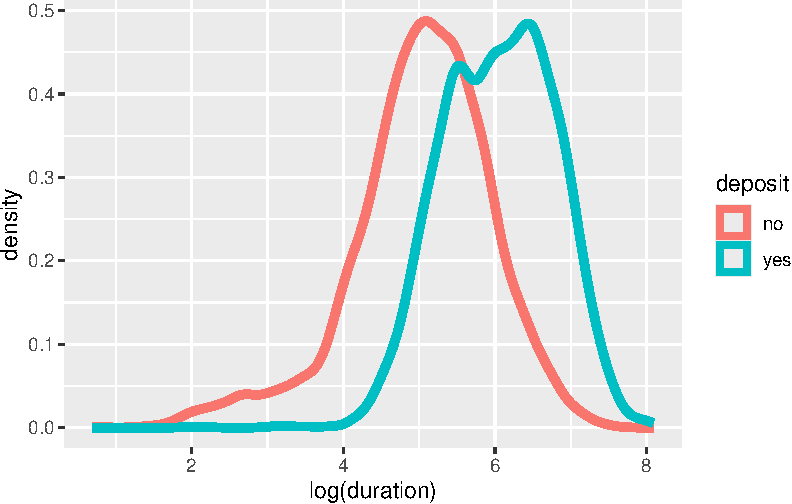
\includegraphics{eda_files/figure-pdf/unnamed-chunk-23-1.pdf}

}

\end{figure}

Puede observarse una relación. Valores altos de la variable
\texttt{duración} parecen estar relacionados con observaciones con
\texttt{deposit} igual a `yes'.

\begin{Shaded}
\begin{Highlighting}[]
\NormalTok{df }\OtherTok{=}\NormalTok{ bank.train }\SpecialCharTok{\%\textgreater{}\%} 
      \FunctionTok{select}\NormalTok{(duration,deposit)}\SpecialCharTok{\%\textgreater{}\%}
      \FunctionTok{mutate}\NormalTok{(}\AttributeTok{log.duration=}\FunctionTok{log}\NormalTok{(duration))}

\CommentTok{\# Resumen para los casos de depósito}
\FunctionTok{summary}\NormalTok{(df }\SpecialCharTok{\%\textgreater{}\%} \FunctionTok{filter}\NormalTok{(deposit}\SpecialCharTok{==}\StringTok{"yes"}\NormalTok{) }\SpecialCharTok{\%\textgreater{}\%}\NormalTok{ .}\SpecialCharTok{$}\NormalTok{log.duration)}
\end{Highlighting}
\end{Shaded}

\begin{verbatim}
   Min. 1st Qu.  Median    Mean 3rd Qu.    Max. 
  2.079   5.497   6.073   6.046   6.593   8.087 
\end{verbatim}

\begin{Shaded}
\begin{Highlighting}[]
\CommentTok{\# Resumen para los casos de no depósito}
\FunctionTok{summary}\NormalTok{(df }\SpecialCharTok{\%\textgreater{}\%} \FunctionTok{filter}\NormalTok{(deposit}\SpecialCharTok{==}\StringTok{"no"}\NormalTok{) }\SpecialCharTok{\%\textgreater{}\%}\NormalTok{ .}\SpecialCharTok{$}\NormalTok{log.duration)}
\end{Highlighting}
\end{Shaded}

\begin{verbatim}
   Min. 1st Qu.  Median    Mean 3rd Qu.    Max. 
 0.6931  4.5433  5.0999  5.0308  5.6276  7.5022 
\end{verbatim}

Gráficamente, podemos comparar los boxplots.

\begin{Shaded}
\begin{Highlighting}[]
\FunctionTok{ggplot}\NormalTok{(df, }\FunctionTok{aes}\NormalTok{(deposit, log.duration)) }\SpecialCharTok{+}
        \FunctionTok{geom\_boxplot}\NormalTok{()}
\end{Highlighting}
\end{Shaded}

\begin{figure}[H]

{\centering 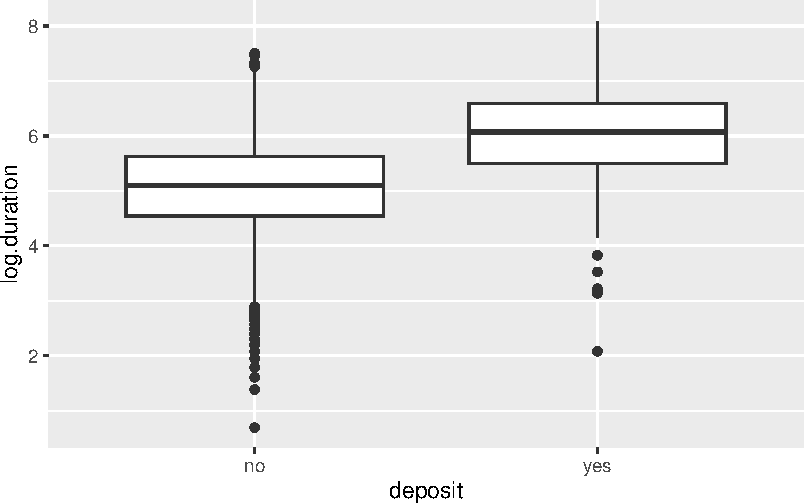
\includegraphics{eda_files/figure-pdf/unnamed-chunk-25-1.pdf}

}

\end{figure}

Podemos determinar la importancia de relación. Por ejemplo, podemos
realizar un test de la T para igualdad de medias. Estudiaremos estos
conceptos en el Chapter~\ref{sec-para}.

\begin{Shaded}
\begin{Highlighting}[]
\FunctionTok{t.test}\NormalTok{(log.duration }\SpecialCharTok{\textasciitilde{}}\NormalTok{ deposit, }\AttributeTok{data =}\NormalTok{ df)}
\end{Highlighting}
\end{Shaded}

\begin{verbatim}

    Welch Two Sample t-test

data:  log.duration by deposit
t = -45.828, df = 5464.5, p-value < 2.2e-16
alternative hypothesis: true difference in means between group no and group yes is not equal to 0
95 percent confidence interval:
 -1.0583835 -0.9715488
sample estimates:
 mean in group no mean in group yes 
         5.030821          6.045787 
\end{verbatim}

\begin{tcolorbox}[enhanced jigsaw, arc=.35mm, breakable, coltitle=black, left=2mm, opacityback=0, bottomtitle=1mm, colbacktitle=quarto-callout-caution-color!10!white, title=\textcolor{quarto-callout-caution-color}{\faFire}\hspace{0.5em}{Ejercicio}, titlerule=0mm, colback=white, colframe=quarto-callout-caution-color-frame, bottomrule=.15mm, rightrule=.15mm, opacitybacktitle=0.6, toptitle=1mm, toprule=.15mm, leftrule=.75mm]

Comprenderás este resultado a lo largo del curso. De momento, puedes
preguntar al profesor. Dejamos como ejercicio para el alumno la
interpretación del resultado del test.

\end{tcolorbox}

Es posible estudiar la relación entre dos variables categóricas de
manera gráfica.

\begin{Shaded}
\begin{Highlighting}[]
\FunctionTok{ggplot}\NormalTok{(}\AttributeTok{data =}\NormalTok{ bank.train, }\FunctionTok{aes}\NormalTok{(}\AttributeTok{x =}\NormalTok{ housing, }\AttributeTok{fill =}\NormalTok{ deposit)) }\SpecialCharTok{+}
    \FunctionTok{geom\_bar}\NormalTok{()}
\end{Highlighting}
\end{Shaded}

\begin{figure}[H]

{\centering 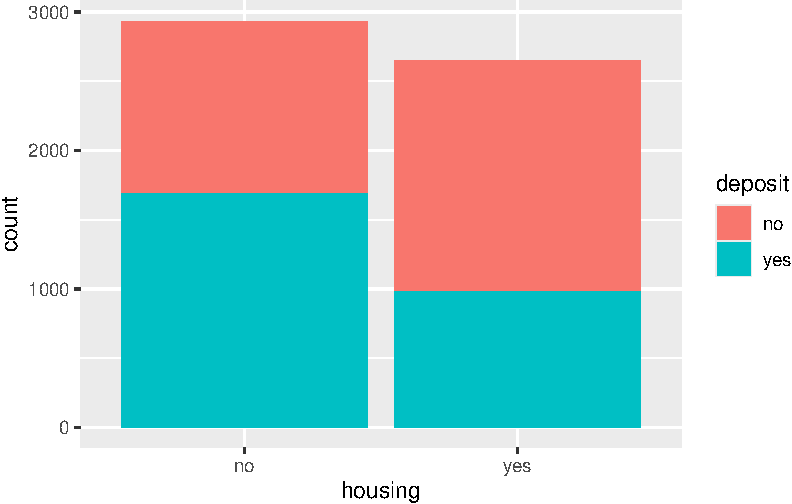
\includegraphics{eda_files/figure-pdf/unnamed-chunk-27-1.pdf}

}

\end{figure}

Parece haber una relación, estando asociados las observaciones de
personas con casa propia a un mayor porcentaje de `no' en la variable
respuesta. Podemos obtener la tabla de contingencia:

\begin{Shaded}
\begin{Highlighting}[]
\NormalTok{data1}\OtherTok{=}\FunctionTok{table}\NormalTok{(bank.train}\SpecialCharTok{$}\NormalTok{housing, bank.train}\SpecialCharTok{$}\NormalTok{deposit)}


\FunctionTok{dimnames}\NormalTok{(data1) }\OtherTok{\textless{}{-}} \FunctionTok{list}\NormalTok{(}\AttributeTok{housing =} \FunctionTok{c}\NormalTok{(}\StringTok{"no"}\NormalTok{, }\StringTok{"yes"}\NormalTok{),}
                        \AttributeTok{deposit =} \FunctionTok{c}\NormalTok{(}\StringTok{"no"}\NormalTok{, }\StringTok{"yes"}\NormalTok{))}
\NormalTok{data1}
\end{Highlighting}
\end{Shaded}

\begin{verbatim}
       deposit
housing   no  yes
    no  1246 1688
    yes 1662  985
\end{verbatim}

Y el contraste correspondiente para la hipótesis nula de no existencia
de relación. Estudiaremos estos conceptos en el Chapter~\ref{sec-para}.

\begin{Shaded}
\begin{Highlighting}[]
\FunctionTok{chisq.test}\NormalTok{(bank.train}\SpecialCharTok{$}\NormalTok{housing, bank.train}\SpecialCharTok{$}\NormalTok{deposit)}
\end{Highlighting}
\end{Shaded}

\begin{verbatim}

    Pearson's Chi-squared test with Yates' continuity correction

data:  bank.train$housing and bank.train$deposit
X-squared = 229.44, df = 1, p-value < 2.2e-16
\end{verbatim}

\begin{tcolorbox}[enhanced jigsaw, arc=.35mm, breakable, coltitle=black, left=2mm, opacityback=0, bottomtitle=1mm, colbacktitle=quarto-callout-caution-color!10!white, title=\textcolor{quarto-callout-caution-color}{\faFire}\hspace{0.5em}{Ejercicio}, titlerule=0mm, colback=white, colframe=quarto-callout-caution-color-frame, bottomrule=.15mm, rightrule=.15mm, opacitybacktitle=0.6, toptitle=1mm, toprule=.15mm, leftrule=.75mm]

Dejamos como ejercicio para el alumno la interpretación del resultado
del test.

\end{tcolorbox}

\bookmarksetup{startatroot}

\hypertarget{sec-para}{%
\chapter{Estimación y contraste paramétrico}\label{sec-para}}

\hypertarget{definiciuxf3n-de-estaduxedstico}{%
\section{Definición de
estadístico}\label{definiciuxf3n-de-estaduxedstico}}

Un \textbf{estadístico} es una medida calculada a partir de una muestra
de datos que se utiliza para describir o resumir características de la
muestra. En otras palabras, un estadístico es un valor numérico que
resume o describe algún aspecto de los datos recolectados. Los
estadísticos se utilizan ampliamente en análisis de datos, inferencia
estadística y para hacer estimaciones sobre poblaciones más grandes
basadas en la información obtenida de una muestra.

Como puedes ver, en la Chapter~\ref{sec-eda} hemos estado trabajando con
estadísticos. Los estadísticos juegan un papel crucial en la inferencia
estadística, donde se utilizan para hacer estimaciones o probar
hipótesis sobre una población a partir de la información contenida en
una muestra.

Ejemplos comunes de estadísticos incluyen:

\begin{itemize}
\tightlist
\item
  Media: Promedio aritmético de los valores en la muestra.
\item
  Mediana: Valor que divide la muestra en dos partes iguales.
\item
  Moda: Valor que aparece con mayor frecuencia en la muestra.
\item
  Varianza: Medida de la dispersión de los datos respecto a la media.
\item
  Desviación estándar: Raíz cuadrada de la varianza, que también mide la
  dispersión.
\item
  Coeficiente de correlación: Medida de la relación entre dos variables.
\end{itemize}

\hypertarget{estimaciuxf3n-puntual-1}{%
\section{Estimación puntual}\label{estimaciuxf3n-puntual-1}}

La \textbf{estimación puntual} es una técnica en estadística que
consiste en utilizar los datos de una muestra para calcular un valor
único, denominado \textbf{estimador puntual}, que se usa como mejor
aproximación de un parámetro desconocido de la población. Este parámetro
puede ser, por ejemplo, la media, la varianza, la proporción, entre
otros. La estimación puntual proporciona una forma simple y directa de
hacer inferencias sobre parámetros poblacionales a partir de una
muestra, aunque su simplicidad también implica que no proporciona
información sobre la precisión o variabilidad de la estimación, aspectos
que se abordan mediante la \textbf{estimación por intervalos} y otras
técnicas inferenciales.

\hypertarget{conceptos-clave-en-la-estimaciuxf3n-puntual}{%
\subsection{Conceptos Clave en la Estimación
Puntual}\label{conceptos-clave-en-la-estimaciuxf3n-puntual}}

\textbf{Estimador}: Es una fórmula o función que se aplica a los datos
de la muestra para obtener la estimación puntual. Por ejemplo, la media
muestral (\(\bar{x}\)) es un estimador de la media poblacional
(\(\mu\)).

\textbf{Estimación}: Es el valor numérico específico obtenido al aplicar
el estimador a una muestra concreta de datos. Por ejemplo, si
\(\bar{x} = 5.4\), esa es la estimación puntual de \(\mu\).

\hypertarget{ejemplos-de-estimadores-puntuales}{%
\subsection{Ejemplos de Estimadores
Puntuales}\label{ejemplos-de-estimadores-puntuales}}

\begin{itemize}
\item
  \textbf{Media Muestral (}\(\bar{x}\)): Utilizada para estimar la media
  poblacional (\(\mu\)). \[
  \bar{x} = \frac{1}{n} \sum_{i=1}^n x_i
  \]
\item
  \textbf{Varianza Muestral (}\(s^2\)): Utilizada para estimar la
  varianza poblacional (\(\sigma^2\)). \[
  s^2 = \frac{1}{n-1} \sum_{i=1}^n (x_i - \bar{x})^2
  \]
\item
  \textbf{Proporción Muestral (}\(\hat{p}\)): Utilizada para estimar la
  proporción poblacional (\(p\)). \[
  \hat{p} = \frac{x}{n}
  \] donde \(x\) es el número de éxitos en la muestra y \(n\) es el
  tamaño de la muestra.
\end{itemize}

\hypertarget{propiedades-de-los-estimadores}{%
\section{Propiedades de los
estimadores}\label{propiedades-de-los-estimadores}}

Existen diferentes métodos diferentes para obtener estimadores de un
parámetro poblacional. ¿Cómo elegir el estimador más adecuado para un
parámetro desconocid? ¿Cuáles son las propiedades de un buen estimador?

Para que un estimador sea considerado adecuado, generalmente debe
cumplir con ciertas propiedades:

\begin{itemize}
\tightlist
\item
  \textbf{Insesgadez}: Un estimador es insesgado si, en promedio,
  coincide con el valor verdadero del parámetro que se estima. Es decir,
  el valor esperado del estimador es igual al parámetro poblacional.
\end{itemize}

\[E(\hat{\theta}) = \theta\] La comparaciones que implican estimadores
sesgados a menudo se basan en el \emph{error cuadrático medio} definido
como: \[
ECM(\hat{\theta})=E[(\hat{\theta}- \theta)^2]=Var(\hat{\theta})+(E(\hat{\theta})- \theta)^2=Eficiencia+  Sesgo
\] En este grado vas a volver a oir hablar de esta medida en la
asignatura de regresión. En ese caso, la medida de error más empleada
es: \[
ECM=\frac{1}{n}\sum_{i=1}^n(y_i-\hat{f}(x_i))^2
\] donde \(\hat{f}(x_i)\) e sla predicción que hace un modelo de
regresión mediante una función \(\hat{f}\) para la i-ésima observación
muestral \(x_i\).

\begin{itemize}
\item
  \textbf{Consistencia}: Un estimador es consistente si, a medida que el
  tamaño de la muestra aumenta, la estimación se aproxima al valor
  verdadero del parámetro. Es decir: \[
  lim_{n  \rightarrow \infty}P(|\hat{\theta}-\theta|\geq\delta)=0, \forall\delta>0
  \] donde \(n\) es el tamaño muestral.
\item
  \textbf{Eficiencia}: La varianza de un estimador debe ser lo más
  pequeña posible. Entre dos estimadores insesgados, el más eficiente es
  el que tiene menor varianza, es decir, el que proporciona estimaciones
  más precisas.
\item
  \textbf{Suficiencia}: Un estimador es suficiente si utiliza toda la
  información contenida en la muestra sobre el parámetro que se está
  estimando.
\end{itemize}

\begin{tcolorbox}[enhanced jigsaw, arc=.35mm, breakable, coltitle=black, left=2mm, opacityback=0, bottomtitle=1mm, colbacktitle=quarto-callout-tip-color!10!white, title=\textcolor{quarto-callout-tip-color}{\faLightbulb}\hspace{0.5em}{Ejemplo Práctico. Insesgadez}, titlerule=0mm, colback=white, colframe=quarto-callout-tip-color-frame, bottomrule=.15mm, rightrule=.15mm, opacitybacktitle=0.6, toptitle=1mm, toprule=.15mm, leftrule=.75mm]

Para entender la propiedad de insesgadez en inferencia estadística, es
útil realizar una simulación en \texttt{R}. Como hemos visto, la
insesgadez de un estimador significa que, en promedio, el estimador
coincide con el parámetro verdadero de la población.

Vamos a realizar una simulación para ilustrar esta propiedad utilizando
la media muestral como estimador de la media poblacional. Generaremos
muchas muestras aleatorias de una distribución normal y compararemos la
media de las medias muestrales con la media verdadera de la población.

\begin{Shaded}
\begin{Highlighting}[]
\CommentTok{\# Cargar la librería ggplot2}
\FunctionTok{library}\NormalTok{(ggplot2)}

\CommentTok{\# Parámetros de la simulación}
\FunctionTok{set.seed}\NormalTok{(}\DecValTok{123}\NormalTok{)  }\CommentTok{\# Para reproducibilidad}
\NormalTok{n\_muestras }\OtherTok{\textless{}{-}} \DecValTok{1000}  \CommentTok{\# Número de muestras}
\NormalTok{tamano\_muestra }\OtherTok{\textless{}{-}} \DecValTok{30}  \CommentTok{\# Tamaño de cada muestra}
\NormalTok{media\_poblacional }\OtherTok{\textless{}{-}} \DecValTok{50}  \CommentTok{\# Media verdadera de la población}
\NormalTok{desviacion\_estandar }\OtherTok{\textless{}{-}} \DecValTok{10}  \CommentTok{\# Desviación estándar de la población}

\CommentTok{\# Generar muestras y calcular medias muestrales}
\NormalTok{medias\_muestrales }\OtherTok{\textless{}{-}} \FunctionTok{numeric}\NormalTok{(n\_muestras)}
\ControlFlowTok{for}\NormalTok{ (i }\ControlFlowTok{in} \DecValTok{1}\SpecialCharTok{:}\NormalTok{n\_muestras) \{}
\NormalTok{  muestra }\OtherTok{\textless{}{-}} \FunctionTok{rnorm}\NormalTok{(tamano\_muestra, }\AttributeTok{mean =}\NormalTok{ media\_poblacional, }\AttributeTok{sd =}\NormalTok{ desviacion\_estandar)}
\NormalTok{  medias\_muestrales[i] }\OtherTok{\textless{}{-}} \FunctionTok{mean}\NormalTok{(muestra)}
\NormalTok{\}}

\CommentTok{\# Calcular la media de las medias muestrales}
\NormalTok{media\_de\_medias\_muestrales }\OtherTok{\textless{}{-}} \FunctionTok{mean}\NormalTok{(medias\_muestrales)}

\CommentTok{\# Imprimir resultados}
\FunctionTok{cat}\NormalTok{(}\StringTok{"Media verdadera de la población:"}\NormalTok{, media\_poblacional, }\StringTok{"}\SpecialCharTok{\textbackslash{}n}\StringTok{"}\NormalTok{)}
\end{Highlighting}
\end{Shaded}

\begin{verbatim}
Media verdadera de la población: 50 
\end{verbatim}

\begin{Shaded}
\begin{Highlighting}[]
\FunctionTok{cat}\NormalTok{(}\StringTok{"Media de las medias muestrales:"}\NormalTok{, media\_de\_medias\_muestrales, }\StringTok{"}\SpecialCharTok{\textbackslash{}n}\StringTok{"}\NormalTok{)}
\end{Highlighting}
\end{Shaded}

\begin{verbatim}
Media de las medias muestrales: 49.93807 
\end{verbatim}

\begin{Shaded}
\begin{Highlighting}[]
\CommentTok{\# Crear un data frame para ggplot}
\NormalTok{datos }\OtherTok{\textless{}{-}} \FunctionTok{data.frame}\NormalTok{(medias\_muestrales)}

\CommentTok{\# Graficar las medias muestrales usando ggplot2}
\FunctionTok{ggplot}\NormalTok{(datos, }\FunctionTok{aes}\NormalTok{(}\AttributeTok{x =}\NormalTok{ medias\_muestrales)) }\SpecialCharTok{+}
  \FunctionTok{geom\_histogram}\NormalTok{(}\AttributeTok{bins =} \DecValTok{30}\NormalTok{, }\AttributeTok{fill =} \StringTok{"lightblue"}\NormalTok{, }\AttributeTok{color =} \StringTok{"black"}\NormalTok{, }\AttributeTok{alpha =} \FloatTok{0.7}\NormalTok{) }\SpecialCharTok{+}
  \FunctionTok{geom\_vline}\NormalTok{(}\FunctionTok{aes}\NormalTok{(}\AttributeTok{xintercept =}\NormalTok{ media\_poblacional), }\AttributeTok{color =} \StringTok{"red"}\NormalTok{, }\AttributeTok{linetype =} \StringTok{"dashed"}\NormalTok{, }\AttributeTok{size =} \FloatTok{1.2}\NormalTok{) }\SpecialCharTok{+}
  \FunctionTok{geom\_vline}\NormalTok{(}\FunctionTok{aes}\NormalTok{(}\AttributeTok{xintercept =}\NormalTok{ media\_de\_medias\_muestrales), }\AttributeTok{color =} \StringTok{"blue"}\NormalTok{, }\AttributeTok{linetype =} \StringTok{"dashed"}\NormalTok{, }\AttributeTok{size =} \FloatTok{1.2}\NormalTok{) }\SpecialCharTok{+}
  \FunctionTok{labs}\NormalTok{(}\AttributeTok{title =} \StringTok{"Distribución de las Medias Muestrales"}\NormalTok{,}
       \AttributeTok{x =} \StringTok{"Medias Muestrales"}\NormalTok{,}
       \AttributeTok{y =} \StringTok{"Frecuencia"}\NormalTok{) }\SpecialCharTok{+}
  \FunctionTok{theme\_minimal}\NormalTok{() }\SpecialCharTok{+}
  \FunctionTok{theme}\NormalTok{(}\AttributeTok{plot.title =} \FunctionTok{element\_text}\NormalTok{(}\AttributeTok{hjust =} \FloatTok{0.5}\NormalTok{)) }\SpecialCharTok{+}
  \FunctionTok{annotate}\NormalTok{(}\StringTok{"text"}\NormalTok{, }\AttributeTok{x =}\NormalTok{ media\_poblacional, }\AttributeTok{y =} \FunctionTok{max}\NormalTok{(}\FunctionTok{table}\NormalTok{(datos}\SpecialCharTok{$}\NormalTok{medias\_muestrales)) }\SpecialCharTok{*} \FloatTok{0.9}\NormalTok{, }\AttributeTok{label =} \StringTok{"Media Verdadera"}\NormalTok{, }\AttributeTok{color =} \StringTok{"red"}\NormalTok{, }\AttributeTok{angle =} \DecValTok{90}\NormalTok{, }\AttributeTok{vjust =} \SpecialCharTok{{-}}\FloatTok{0.5}\NormalTok{) }\SpecialCharTok{+}
  \FunctionTok{annotate}\NormalTok{(}\StringTok{"text"}\NormalTok{, }\AttributeTok{x =}\NormalTok{ media\_de\_medias\_muestrales, }\AttributeTok{y =} \FunctionTok{max}\NormalTok{(}\FunctionTok{table}\NormalTok{(datos}\SpecialCharTok{$}\NormalTok{medias\_muestrales)) }\SpecialCharTok{*} \FloatTok{0.9}\NormalTok{, }\AttributeTok{label =} \StringTok{"Media de las Medias Muestrales"}\NormalTok{, }\AttributeTok{color =} \StringTok{"blue"}\NormalTok{, }\AttributeTok{angle =} \DecValTok{90}\NormalTok{, }\AttributeTok{vjust =} \FloatTok{1.5}\NormalTok{)}
\end{Highlighting}
\end{Shaded}

\begin{verbatim}
Warning: Using `size` aesthetic for lines was deprecated in ggplot2 3.4.0.
i Please use `linewidth` instead.
\end{verbatim}

\begin{figure}[H]

{\centering 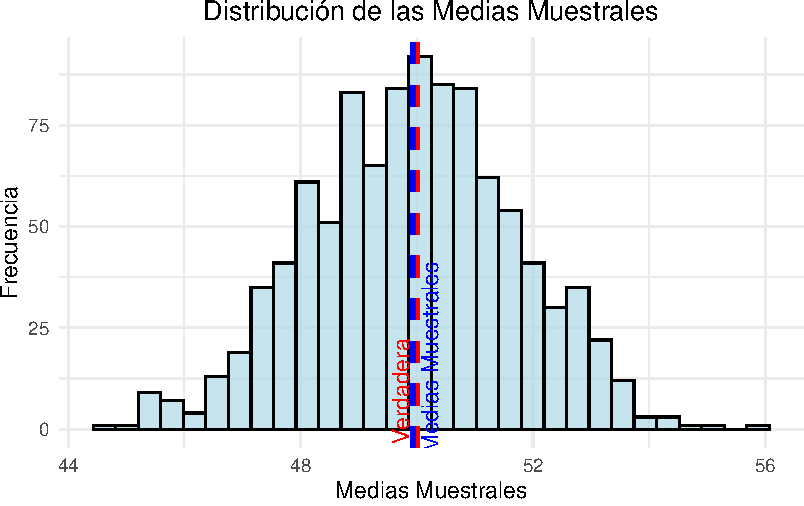
\includegraphics{para_files/figure-pdf/inses1-1.pdf}

}

\end{figure}

Hemos creado un bucle para generar \texttt{n\_muestras} muestras
aleatorias de una distribución normal con la media y desviación estándar
especificadas. Para cada muestra, calculamos la media muestral y la
almacenamos en el vector \texttt{medias\_muestrales}. Calculamos la
media de todas las medias muestrales generadas y mostramos la media
verdadera de la población y la media de las medias muestrales.

El gráfico resultante muestra un histograma de las medias muestrales con
líneas verticales indicando la media verdadera de la población y la
media de las medias muestrales. Esto ilustra visualmente la propiedad de
insesgadez del estimador de la media.

\end{tcolorbox}

\hypertarget{muxe9todo-de-los-momentos}{%
\section{Método de los momentos}\label{muxe9todo-de-los-momentos}}

El método de los momentos es una técnica utilizada en estadística para
estimar los parámetros desconocidos de una distribución de probabilidad.
Fue introducido por el estadístico \emph{Karl Pearson} en 1984. Este
método se basa en igualar los momentos muestrales (calculados a partir
de los datos observados) con los momentos teóricos (expresados en
términos de los parámetros de la distribución).

\hypertarget{definiciuxf3n-de-momentos}{%
\subsection{Definición de Momentos}\label{definiciuxf3n-de-momentos}}

En estadística, los \textbf{momentos} de una distribución son medidas
que describen diversas características de la distribución, como su
media, varianza, simetría y curtosis. Los momentos más comunes son:

\begin{enumerate}
\def\labelenumi{\arabic{enumi}.}
\tightlist
\item
  \textbf{Primer Momento (Media)}: \(\mu = E[X]\)
\item
  \textbf{Segundo Momento (Varianza)}:\(\mu_2 = E[X^2]\)
\item
  \textbf{Tercer Momento (Asimetría)}:\(\mu_3 = E[X^3]\)
\item
  \textbf{Cuarto Momento (Curtosis)}:\(\mu_4 = E[X^4]\)
\end{enumerate}

\begin{enumerate}
\def\labelenumi{\alph{enumi}.}
\setcounter{enumi}{10}
\tightlist
\item
  \textbf{k-esimo Momento}:\(\mu_k = E[X^k]\)
\end{enumerate}

Los momentos poblacionales pueden ser vistos como funciones de los
parámetros desconocidos \(\theta_1,\ldots,\theta_k\). Se asume que se
conoce el modelo de probabilidad de la variable objeto de estudio.

\hypertarget{pasos-del-muxe9todo-de-los-momentos}{%
\subsection{Pasos del Método de los
Momentos}\label{pasos-del-muxe9todo-de-los-momentos}}

El método de los momentos consiste en resolver un conjunto de ecuaciones
y tiene los siguientes pasos:

\begin{enumerate}
\def\labelenumi{\arabic{enumi}.}
\item
  \textbf{Calcular Momentos Muestrales}: Se calculan los momentos
  muestrales de los datos observados. El (k)-ésimo momento muestral se
  define como: \(m_k = \frac{1}{n} \sum_{i=1}^{n}X_i^k\) donde \(n\) es
  el tamaño de la muestra y \(X_i\) son los valores de la muestra.
\item
  \textbf{Igualar Momentos Muestrales y Teóricos}: Se igualan los
  momentos muestrales con los momentos teóricos de la distribución. Los
  momentos teóricos se expresan en términos de los parámetros
  desconocidos que se desean estimar.
\item
  \textbf{Resolver el Sistema de Ecuaciones}: Se resuelve el sistema de
  ecuaciones resultante para encontrar los estimadores de los parámetros
  desconocidos. Fíjate que tenemos \(k\) ecuaciones y \(k\) parámetros
  (\(\theta_1,\ldots,\theta_k\)). De modo que es posible despejar los
  parámetros de estas ecuaciones, que quedando estos parámetros en
  función de los momentos. En estas ecuaciones se sustituyen los
  momentos poblacionales por sus correspondientes momentos
  poblacionales. Esto da como resultado estimaciones de esos parámetros.
\end{enumerate}

\begin{tcolorbox}[enhanced jigsaw, arc=.35mm, breakable, coltitle=black, left=2mm, opacityback=0, bottomtitle=1mm, colbacktitle=quarto-callout-tip-color!10!white, title=\textcolor{quarto-callout-tip-color}{\faLightbulb}\hspace{0.5em}{Ejemplo, distribución Normal}, titlerule=0mm, colback=white, colframe=quarto-callout-tip-color-frame, bottomrule=.15mm, rightrule=.15mm, opacitybacktitle=0.6, toptitle=1mm, toprule=.15mm, leftrule=.75mm]

Supongamos que deseamos estimar los parámetros (\(\mu\)) y
(\(\sigma^2\)) de una distribución Normal (\(N(\mu, \sigma^2)\)).

\begin{enumerate}
\def\labelenumi{\arabic{enumi}.}
\item
  \textbf{Calcular los momentos muestrales}:
  \[m_1 = \frac{1}{n} \sum_{i=1}^n X_i \]
  \[m_2 = \frac{1}{n}\sum_{i=1}^nX_i^2 \]
\item
  \textbf{Igualar los momentos muestrales con los momentos teóricos}:
  Para una distribución Normal, el primer momento teórico (media) es
\end{enumerate}

\[\mu_1=E(X)=\mu\]

y el segundo momento teórico es:

\[\mu_2=E(X^2)=Var(X)+E(X)^2=\mu^2 + \sigma^2\]

Igualando estos con los momentos muestrales obtenidos de los datos:
\[m_1 = \bar{X}=\mu\]
\[m_2 = \frac{1}{n}\sum_{i=1}^n X_i^2=\mu_2= \mu^2 + \sigma^2\]

\begin{enumerate}
\def\labelenumi{\arabic{enumi}.}
\setcounter{enumi}{2}
\tightlist
\item
  \textbf{Resolver el sistema de ecuaciones}: De la primera ecuación,
  tenemos:
\end{enumerate}

\[\hat{\mu} = \bar{X}\]

Sustituyendo en la segunda ecuación:
\[\hat{\sigma}^2=\frac{1}{n}\sum_{i=1}^n X_i^2-\bar{X}^2=\frac{1}{n}\sum_{i=1}^n (X_i-\bar{X})^2\]

Que son los estimadores de los parámetros.

\end{tcolorbox}

\begin{tcolorbox}[enhanced jigsaw, arc=.35mm, breakable, coltitle=black, left=2mm, opacityback=0, bottomtitle=1mm, colbacktitle=quarto-callout-tip-color!10!white, title=\textcolor{quarto-callout-tip-color}{\faLightbulb}\hspace{0.5em}{Ejemplo, distribución Binomial}, titlerule=0mm, colback=white, colframe=quarto-callout-tip-color-frame, bottomrule=.15mm, rightrule=.15mm, opacitybacktitle=0.6, toptitle=1mm, toprule=.15mm, leftrule=.75mm]

Sea \(X_1,\ldots,X_n\) una muestra aleatoria simple de una
\(Binom(k,p)\), con \(k\) y \(p\) desconocidos. Entonces, los momentos
poblacionales son:

\[\mu_1=E(X)=kp\] \[\mu_2=E(X^2)=Var(X)+E(X)^2=kp(1-p)+k^2p^2\] Los
momentos muestrales son:

\[
m_1=\bar{X}
\] \[
m_2=\frac{1}{n}\sum_{i=1}^nX_i^2
\] Igualando los momentos poblacionales a los muestrales, obtenemos:

\[
m_1=\bar{X}=kp
\]

\[
m_2=\frac{1}{n}\sum_{i=1}^nX_i^2=\mu_2=kp(1-p)+k^2p^2
\] Despejando \(k\) y \(p\), obtenemos los estimadores:

\[
\hat{k}^2=\frac{\bar{X}^2}{\bar{X}-(1/n)\sum_{i=1}^n(X_i- \bar{X})^2}
\] \[\hat{p}=\frac{\bar{X}}{\hat{k}}\]

\end{tcolorbox}

\hypertarget{ventajas-y-limitaciones}{%
\subsection{Ventajas y Limitaciones}\label{ventajas-y-limitaciones}}

Los estimadores de los momentos presentan interesantes propiedades
estadísticas, aunqeu también tienen sus limitaciones.

\textbf{Ventajas}:

\begin{itemize}
\tightlist
\item
  \textbf{Simplicidad}: El método de los momentos es relativamente
  sencillo de aplicar y no requiere técnicas complejas de optimización.
\item
  \textbf{Intuición}: Ofrece una interpretación intuitiva de los
  parámetros en términos de momentos.
\end{itemize}

\textbf{Limitaciones}:

\begin{itemize}
\tightlist
\item
  \textbf{Precisión}: Los estimadores de los momentos no siempre son los
  estimadores más eficientes (no tienen la mínima varianza posible).
\item
  \textbf{Aplicabilidad}: En algunas distribuciones complejas, los
  momentos pueden no existir o ser difíciles de calcular.
\item
  \textbf{Consistencia}: Los estimadores de momentos no siempre son
  consistentes, especialmente en muestras pequeñas.
\end{itemize}

\hypertarget{muxe9todo-de-la-muxe1xima-verosimilud}{%
\section{Método de la máxima
verosimilud}\label{muxe9todo-de-la-muxe1xima-verosimilud}}

El método de la máxima verosimilitud es una técnica estadística
ampliamente utilizada para estimar los parámetros desconocidos de una
distribución de probabilidad. Este método se basa en encontrar los
valores de los parámetros que maximicen la función de verosimilitud, la
cual mide la probabilidad de observar los datos dados los parámetros. El
método de m-axima verosimilitud es el método más popular para obtener un
estimador. La idea básica es seleccionar el valor del parámetro que hace
que los datos sean más probables.

Dado un modelo estadiıstico (es decir, una familia de distribuciones
\(f(·|\theta)| \theta \in \Theta\) donde \(\theta\) es el parámetro del
modelo), el método de máxima verosimilitud encuentra el valor del
parámetro del modelo \(\theta\) que maximiza la función de
verosimilitud:

\[
\hat{\theta}(x)= \max_{\theta \in \Theta}L(\theta|\mathbf{x})
\]

Para una muestra aleatoria \(\mathbf{x}=(x_1,\ldots,x_n)\) de una
variable aleatoria \(X\), la \emph{verosimilitud} es proporcional al
producto de las probabilidades asociadas a los valores individuales: \[
\prod_jP(X=x_j)
\] El término fue acuñado por Sir Roland Fisher.

Cuando \(X\) es una variable aleatoria continua, un valor muestral
\(x_j\) debe considerarse como que está (en general) en el intervalo
\((x_j-\delta,x_j+\delta)\), donde \(\delta\) representa la precisión de
la medición. La verosimilutd es entonces proporcional a: \[
\prod_jP(x_j-\delta<X<x_j+\delta).
\] Si \(\delta\) es suficientemente pequeño, esta expresión es
aproximadamente proporcional a: \[
\prod_jf(x_j).
\] donde \(f\) es la función de densidad de \(X\). Por lo tanto, la
\emph{verosimilitd} describe lo plausible que es un valor del parámetro
poblacional, dadas unas observaciones concretas de la muestra.

\hypertarget{conceptos-buxe1sicos}{%
\subsection{Conceptos Básicos}\label{conceptos-buxe1sicos}}

\begin{enumerate}
\def\labelenumi{\arabic{enumi}.}
\item
  \textbf{Función de Verosimilitud}: La función de verosimilitud,
  \(L(\theta|\mathbf{x})\), para un conjunto de datos
  \(\mathbf{x} = (x_1, x_2, \ldots, x_n)\) y un vector de parámetros
  \(\theta\), es el producto de las funciones de densidad (o de
  probabilidad) de los datos observados, dadas las posibles
  realizaciones de \(\theta\): \[
  L(\theta|\mathbf{x}) = f(\mathbf{x}|\theta)=f(x_1,\ldots,x_n|\theta)=f(x_1|\theta)f(x_2|\theta)\ldots f(x_n|\theta)=\prod_{i=1}^n f(x_i| \theta)
  \] donde \(f(x_i|\theta)\) es la función de densidad (o de
  probabilidad) de \(x_i\) dado \(\theta\).
\item
  \textbf{Log-Verosimilitud}: Debido a que la función de verosimilitud
  puede implicar productos de muchos términos, es más práctico trabajar
  con su logaritmo natural, conocido como la log-verosimilitud: \[
  \ell(\theta|\mathbf{x}) = \log L(\theta|\mathbf{x}) = \sum_{i=1}^n \log f(x_i|\theta)
  \]
\end{enumerate}

\hypertarget{procedimiento-del-muxe9todo-de-muxe1xima-verosimilitud}{%
\subsection{Procedimiento del Método de Máxima
Verosimilitud}\label{procedimiento-del-muxe9todo-de-muxe1xima-verosimilitud}}

\begin{enumerate}
\def\labelenumi{\arabic{enumi}.}
\item
  \textbf{Especificar la Función de Verosimilitud}: Identificar la
  función de verosimilitud correspondiente a los datos observados y a la
  distribución supuesta.
\item
  \textbf{Calcular la Log-Verosimilitud}: Tomar el logaritmo natural de
  la función de verosimilitud para obtener la función de
  log-verosimilitud.
\item
  \textbf{Derivar y Resolver}: Derivar la función de log-verosimilitud
  con respecto a cada parámetro y resolver las ecuaciones obtenidas
  igualando a cero (puntos críticos) para encontrar los estimadores de
  máxima verosimilitud (EMV).
\item
  \textbf{Verificar Máximos}: Asegurarse de que las soluciones
  encontradas corresponden a máximos y no a mínimos o puntos de
  inflexión, típicamente verificando la segunda derivada.
\end{enumerate}

\begin{tcolorbox}[enhanced jigsaw, arc=.35mm, breakable, coltitle=black, left=2mm, opacityback=0, bottomtitle=1mm, colbacktitle=quarto-callout-tip-color!10!white, title=\textcolor{quarto-callout-tip-color}{\faLightbulb}\hspace{0.5em}{Ejemplo, distribución Normal}, titlerule=0mm, colback=white, colframe=quarto-callout-tip-color-frame, bottomrule=.15mm, rightrule=.15mm, opacitybacktitle=0.6, toptitle=1mm, toprule=.15mm, leftrule=.75mm]

Supongamos que tenemos una muestra
\(\mathbf{x} = (x_1, x_2, \ldots, x_n)\) de una distribución Normal con
media \(\mu\) y varianza \(\sigma^2\), y queremos estimar estos
parámetros.

\begin{enumerate}
\def\labelenumi{\arabic{enumi}.}
\item
  \textbf{Función de Verosimilitud}: La función de densidad para una
  distribución normal es: \[
  f(x_i|\mu, \sigma^2) = \frac{1}{\sqrt{2\pi\sigma^2}} \exp\left(-\frac{(x_i - \mu)^2}{2\sigma^2}\right)
  \] Por lo tanto, la función de verosimilitud es: \[
  L(\mu, \sigma^2| \mathbf{x}) = \prod_{i=1}^n \frac{1}{\sqrt{2\pi\sigma^2}} \exp\left(-\frac{(x_i - \mu)^2}{2\sigma^2}\right)
  \]
\item
  \textbf{Log-Verosimilitud}: Tomamos el logaritmo natural de la función
  de verosimilitud: \[
  \ell(\mu, \sigma^2|\mathbf{x}) = \sum_{i=1}^n \left[ -\frac{1}{2} \log(2\pi\sigma^2) - \frac{(x_i - \mu)^2}{2\sigma^2} \right]
  \]
\item
  \textbf{Derivadas y Resolución}: Derivamos la log-verosimilitud con
  respecto a \(\mu\) y \(\sigma^2\) y las igualamos a cero: \[
  \frac{\partial \ell}{\partial \mu} = \sum_{i=1}^n \frac{x_i - \mu}{\sigma^2} = 0 \implies \hat{\mu} = \frac{1}{n} \sum_{i=1}^n x_i
  \] \[
  \frac{\partial \ell}{\partial \sigma^2} = -\frac{n}{2\sigma^2} + \frac{1}{2\sigma^4} \sum_{i=1}^n (x_i - \mu)^2 = 0 \implies \hat{\sigma}^2 = \frac{1}{n} \sum_{i=1}^n (x_i - \hat{\mu})^2
  \]

  Así, los estimadores de máxima verosimilitud para \(\mu\) y
  \(\sigma^2\) son la media muestral y la varianza muestral,
  respectivamente.
\end{enumerate}

\end{tcolorbox}

\begin{tcolorbox}[enhanced jigsaw, arc=.35mm, breakable, coltitle=black, left=2mm, opacityback=0, bottomtitle=1mm, colbacktitle=quarto-callout-tip-color!10!white, title=\textcolor{quarto-callout-tip-color}{\faLightbulb}\hspace{0.5em}{Ejemplo, distribución Binomial}, titlerule=0mm, colback=white, colframe=quarto-callout-tip-color-frame, bottomrule=.15mm, rightrule=.15mm, opacitybacktitle=0.6, toptitle=1mm, toprule=.15mm, leftrule=.75mm]

Supongamos que tenemos una muestra de tamaño
\(\mathbf{x} = (x_1, x_2, \ldots, x_n)\) de una variable aleatoria
Binomial con parámetro \(p\) que deseamos estimar. Se emplea dicha
variable para describir el número de errores en las \(n\) pruebas
asociadas. Se realiza un experimento y se obtienen un total de \(4\)
errores en las \(10\) pruebas.

\begin{enumerate}
\def\labelenumi{\arabic{enumi}.}
\tightlist
\item
  \textbf{Función de Verosimilitud}: La verosimilud viene dada por:
\end{enumerate}

\[
L(p|\mathbf{x}) = {10 \choose 4}p^4(1-p)^6
\]

\begin{enumerate}
\def\labelenumi{\arabic{enumi}.}
\setcounter{enumi}{1}
\item
  \textbf{Log-Verosimilitud}: Tomamos el logaritmo natural de la función
  de verosimilitud: \[
  \ell(p|\mathbf{x}) = log\left({10 \choose 4}\right) +4log(p)+6log(1-p)
  \]
\item
  \textbf{Derivadas y Resolución}: Derivamos la log-verosimilitud con
  respecto a \(p\) y las igualamos a cero: \[
  \frac{\partial \ell}{\partial p} =\frac{4}{p} -\frac{6}{1-p}= 0 \implies \frac{4}{p}=\frac{6}{1-p}\implies 4-4p=6p\implies 4=10p \implies p=4/10=0.4
  \]
\end{enumerate}

La función de verosimilud nos informa, dados los datos, sobre los
valores más plausibles (o creíbles) para el parámetroo \(p\).

\end{tcolorbox}

\hypertarget{ventajas-y-limitaciones-1}{%
\subsection{Ventajas y Limitaciones}\label{ventajas-y-limitaciones-1}}

Los estimadores de máxima verosimilutd presentan buenas propiedades
estadísticas.

\textbf{Ventajas}:

\begin{itemize}
\tightlist
\item
  \textbf{Consistencia}: Los estimadores de máxima verosimilitud son
  consistentes, es decir, convergen en probabilidad al valor verdadero
  del parámetro a medida que el tamaño de la muestra aumenta.
\item
  \textbf{Eficiencia}: En muchos casos, los estimadores de máxima
  verosimilitud son eficientes, alcanzando la varianza mínima entre los
  estimadores insesgados (cumplen la igualdad de Cramér-Rao). El
  estimador máximo verosimil es asintóticamente eficiente y su
  distribución converge a la distribución Normal con valor esperado
  \(\theta\) y la varianza es igual al inverso de la información de
  Fisher. La informacioon de Fisher es la cantidad de información que
  una muestra proporciona sobre el valor de un parámetro desconocido.
\item
  \textbf{Flexibilidad}: Se puede aplicar a una amplia gama de
  distribuciones y modelos complejos.
\item
  \textbf{Invariantes}: Si \(T\) es el estimador de máxima verosimilitud
  para \(\theta\), entonces \(\tau(T)\) es el estimador de máxima
  verosimilutd para \(\tau(\theta)\) para cualquier función \(\tau\).
\end{itemize}

\textbf{Limitaciones}:

\begin{itemize}
\tightlist
\item
  \textbf{Complejidad Computacional}: Encontrar los estimadores de
  máxima verosimilitud puede implicar resolver ecuaciones no lineales,
  lo cual puede ser complejo y requerir técnicas numéricas.
\item
  \textbf{Existencia y Unicidad}: Los estimadores de máxima
  verosimilitud no siempre existen y, si existen, no siempre son únicos.
  En problemas reales, la derivada de la función de verosimilitud es, a
  veces, analíticamente intratable. En esos casos, se utilizan métodos
  iterativos para encontrar soluciones numéricas para las estimaciones
  de los parámetros.
\item
  \textbf{Sesgo en Muestras Pequeñas}: Los estimadores pueden ser
  sesgados en muestras pequeñas, aunque el sesgo disminuye a medida que
  el tamaño de la muestra aumenta.
\end{itemize}

\hypertarget{estimaciuxf3n-por-intervalo-1}{%
\section{Estimación por intervalo}\label{estimaciuxf3n-por-intervalo-1}}

La estimación puntual proporciona una aproximación razonable para un
parámetro de la población, pero no tiene en cuenta la variabilidad
debido al tamaño muestral, la variabilidad en la población, el
conocimiento de otros parámetros, etc.

La \textbf{estimación por intervalo} es una técnica en estadística que,
a diferencia de la estimación puntual que proporciona un único valor,
ofrece un rango de valores dentro del cual se espera que se encuentre el
parámetro poblacional desconocido con un cierto nivel de confianza. Este
rango se denomina \textbf{intervalo de confianza}.

La estimación por intervalos es una herramienta esencial en la
inferencia estadística, ya que no solo ofrece una estimación del
parámetro poblacional, sino que también proporciona un marco para
entender la precisión y confiabilidad de esa estimación. Esto la
convierte en una técnica poderosa para hacer inferencias más robustas y
útiles basadas en datos muestrales.

\hypertarget{conceptos-clave-en-la-estimaciuxf3n-por-intervalo}{%
\subsection{Conceptos Clave en la Estimación por
Intervalo}\label{conceptos-clave-en-la-estimaciuxf3n-por-intervalo}}

\textbf{Intervalo de Confianza (IC)}: Es un rango de valores calculado a
partir de los datos de la muestra, que se utiliza para estimar el
parámetro poblacional desconocido. Se expresa comúnmente como
\((\text{Límite Inferior}, \text{Límite Superior})\).

Dada una muestra aleatoria simple \(\mathbf{X}=(X_1,X_2,\ldots,X_n)\) de
una población \(X\) con función de distribución \(F\) que depende de un
parámetro desconocido \(\theta\), diremos que un estimador por
intervalos de confianza del parámetro \(\theta\) con un nivel de
confianza de \((1-\alpha)=100*(1-\alpha)\%\) es un intervalo de la forma
\((T_{inf}(\mathbf{X}),T_{sup}(\mathbf{X}))\) que satisface:
\[P(\theta \in (T_{inf}(\mathbf{X}),T_{sup}(\mathbf{X})))=1-\alpha\]

\textbf{Nivel de Confianza}: Es la probabilidad de que el intervalo de
confianza contenga el verdadero valor del parámetro poblacional. Se
denota como \(1 - \alpha\), donde \(\alpha\) es el nivel de
significancia. Un nivel de confianza común es el \(95\%\), lo que
significa que estamos un \(95\%\) seguros de que el intervalo contiene
el parámetro verdadero. Si repetimos el experimento \(N\) veces, en el
\(95\%\) de las ocasiones el verdadero valor del parámetro estará
incluido en el intervalo proporcionado. Sin embargo es importante
señalar que, dado que el experimento solo suele realizarse en una
ocasión, no podemos estar seguros de que el verdadero valor del
parámetro está incluido en nuestro intervalo. Estará incluido o no
estará incluido, pero no podemos saber en qué situación nos encontramos.
Estar seguro sería tanto como decir que conocemos el verdadero valor del
parámetro. En ese caso, obviamente, no necesitaríamos estimación
ninguna.

\textbf{Error Estándar (SE)}: Es una medida de la variabilidad de un
estimador. Se utiliza para calcular los límites del intervalo de
confianza.

\hypertarget{cuxe1lculo-del-intervalo-de-confianza}{%
\subsection{Cálculo del Intervalo de
Confianza}\label{cuxe1lculo-del-intervalo-de-confianza}}

El cálculo de un intervalo de confianza generalmente sigue la fórmula:

\[
\text{Estimación Puntual} \pm (\text{Valor Crítico} \times \text{Error Estándar})
\] Para alcanzar el intervalo de confianza, generalmente se busca una
cantidad (aletoria) \(C(\mathbf{X},\theta)\) relacionada con el
parámetro desconocido \(\theta\) y con la muestras \(\mathbf{X}\), cuya
distribución sea conocida y no dependa del valor del parámetro. Esta
cantidad recibe el nombre de \emph{pivote} o \emph{cantidad pivotal}
para \(theta\).

Dado que conocemos la distribución del pivote, podemos usar los
cuartiles \(1-\alpha/2\) y \(\alpha/2\) de dicha distribuciuón, y la
desviación estándar dle estimador por intervalos de confianza, para
plantear la siguiente ecuación: \[
P(1-\alpha/2 \text{ cuantil}< C(\mathbf{X},\theta)<\alpha/2 \text{ cuantil}) = 1- \alpha
\] Para obtener los extremos (inferior y superior) del estimador por
intervalos de confianza \(T_{inf}(\mathbf{X})\) y
\(T_{sup}(\mathbf{X})\), se resuelve la doble desigualdad en \(\theta\).
De este modo el intervalo de confianza al \(100(1-\alpha)\%\) para
\(\theta\) es \((T_{inf}(\mathbf{x}),T_{sup}(\mathbf{x}))\)

\hypertarget{importancia-de-la-estimaciuxf3n-por-intervalos}{%
\subsection{Importancia de la Estimación por
Intervalos}\label{importancia-de-la-estimaciuxf3n-por-intervalos}}

A diferencia de la estimación puntual, el intervalo de confianza
proporciona información sobre la precisión de la estimación y la
variabilidad inherente en los datos muestrales.

Además, la estimación por intervalo proporciona un rango de valores que
es útil para la toma de decisiones en el dominio de aplicación.

Podemos señalar que la estimación por intervalos es menos susceptible a
errores muestrales y proporciona una medida más realista del parámetro
poblacional que la obtenida con la estimación puntual.

\hypertarget{intervalo-de-confianza-para-la-media-cuando-la-varianza-es-conocida}{%
\subsection{Intervalo de Confianza para la Media (cuando la varianza es
conocida)}\label{intervalo-de-confianza-para-la-media-cuando-la-varianza-es-conocida}}

Sea una muestra aleatoria simple \(\mathbf{X}\) de tamño \(n\) obtenida
de \(X\). Supongamos que \(X\) sigue una distribución normal con
parámetros (\(\mu\)) y varianza conocida (\(\sigma^2\)). Fijate que este
último supuesto es muy poco realista. El estadístico \(\bar{X}\) tiene
una distribución normal: \[
\bar{X} \sim N \left( \mu,\sigma_{\bar{X}}=\frac{\sigma}{\sqrt{n}}\right )
\] La desviación típica de \(\bar{X}\) ( o de cualquier otro
estadístico) se conoce como su \textbf{error estándar}.

La cantidad pivotal para \(\mu\) es: \[
Z=\frac{\bar{X}-\mu}{\sigma/\sqrt{n}} \sim N \left( 0,1 \right )
\] Ahora, si \(z_{1-\alpha/2}\) y \(z_{\alpha/2}\) son los cuartiles
\((1-alpha/2)\) y \(\alpha/2\) de la distribución \(N(0,1\), entonces
tenemos: \[
P(z_{1-\alpha/2}<Z<z_{\alpha/2})=1-\alpha
\] Es decir: \[
P\left (z_{1-\alpha/2}<\frac{\bar{X}-\mu}{\sigma/\sqrt{n}}<z_{\alpha/2} \right)=1-\alpha
\] Hay que notar que para la distribución Normal:
\(z_{1-\alpha/2}=-z_{\alpha/2}\)

Resolvemos la doble desigualdad para\(\mu\): \[
-z_{\alpha/2}<\frac{\bar{X}-\mu}{\sigma/\sqrt{n}}<z_{\alpha/2} 
\] \[
-z_{\alpha/2}\frac{\sigma}{\sqrt{n}}<\bar{X}-\mu<z_{\alpha/2}\frac{\sigma}{\sqrt{n}} 
\]
\[ -z_{\alpha/2}\frac{\sigma}{\sqrt{n}}-\bar{X}<-\mu<-\bar{X}+z_{\alpha/2}\frac{\sigma}{\sqrt{n}} \]
\[ -z_{\alpha/2}\frac{\sigma}{\sqrt{n}}+\bar{X}>\mu>\bar{X}-z_{\alpha/2}\frac{\sigma}{\sqrt{n}}
\] De modo que el estimador por intervalos de confianza es: \[
\left ( \bar{X}-z_{\alpha/2}\frac{\sigma}{\sqrt{n}},\bar{X}+z_{\alpha/2}\frac{\sigma}{\sqrt{n}} \right)
\] y por tanto, el intervalo de confianza para la media se calcula como:
\[     
IC_{1-\alpha}(\mu)=\left (\bar{x} -z_{\alpha/2} \frac{\sigma}{\sqrt{n}},\bar{x} +z_{\alpha/2}  \frac{\sigma}{\sqrt{n}} \right )= \left( \bar{x} \pm z_{\alpha/2} \frac{\sigma}{\sqrt{n}} \right)
\] donde \(\bar{x}\) es la media muestral, \(z_{\alpha/2}\) es el valor
crítico del estadístico \(z\) para el nivel de confianza deseado,
\(\sigma\) es la desviación estándar poblacional, y \(n\) es el tamaño
de la muestra.

\begin{tcolorbox}[enhanced jigsaw, arc=.35mm, breakable, coltitle=black, left=2mm, opacityback=0, bottomtitle=1mm, colbacktitle=quarto-callout-tip-color!10!white, title=\textcolor{quarto-callout-tip-color}{\faLightbulb}\hspace{0.5em}{Ejemplo. Intervalo de confianza para la media de una distribución normal}, titlerule=0mm, colback=white, colframe=quarto-callout-tip-color-frame, bottomrule=.15mm, rightrule=.15mm, opacitybacktitle=0.6, toptitle=1mm, toprule=.15mm, leftrule=.75mm]

Se ha probado que la altura de los alumnas de primer curso de la URJC se
puede aproximar mediante una variable aleatoria con distribución normal
con desviación típica \(\sigma=10\) cm pero la media \((\mu)\)
desconocida. En un estudio con \(25\) alumnas se obtiene una media de
\(166\) cm. Vamos a construir un intervalo de confianza al \(95\%\) para
\(\mu\).

Sea \(X\) la altura, y sabemos que las variables independientes y
identicamente distribuidas: \[
X_1,X_2,\ldots,X_{50}\sim N(\mu,\sigma^2=10^2).
\] Dado que: \[
\frac{\sigma^2}{n}=\frac{10^2}{50}=2,
\] sabemos que: \[
\bar{X}\sim N(\mu,2),
\] y por tanto: \[
\frac{\bar{X}-\mu}{\sqrt{2}}\sim N(0,1).
\] Además los cuartiles de la distribución normal nos dicen que si
\(Z\sim N(0,1)\), entonces: \[
P(-1,96<Z<1,96)=0,95.
\] Por tanto: \[
P\left(-1,96<\frac{\bar{X}-\mu}{\sqrt{2}}<1,96\right)=0,95.
\] Despejamos \(\mu\):

\[
P\left(\bar{X}-1,96\sqrt{2}<\mu<\bar{X}+1,96\sqrt{2}\right)=0,95.
\] Por tanto, si \(\bar{x}\) es una realización particular de la
variable aleatoria \(\bar{X}\) en la muestra observada, el intervalo de
confianza al \(95\%\) será: \[
IC_{0.5}(\mu)=\bar{x}\pm1.96 \sqrt{2} = \bar{x}\pm2.77
\] En nuestro caso particular como la media era \(\bar{x}=166\) cm,
tenemos: \[
IC_{0.5}(\mu)= 166\pm2.77=(163.23 , 168,77)
\]

\end{tcolorbox}

\hypertarget{intervalo-de-confianza-para-la-media-cuando-la-varianza-es-desconocida}{%
\subsection{Intervalo de Confianza para la media (cuando la varianza es
desconocida)}\label{intervalo-de-confianza-para-la-media-cuando-la-varianza-es-desconocida}}

Sea una muestra aleatoria simple \(\mathbf{X}\) de tamaño \(n\) obtenida
de \(X\). Supongamos que \(X\) sigue una distribución normal con
parámetros (\(\mu\)) y varianza desconocida (\(\sigma^2\)). Este
supuesto es más realista que el caso anterior. Lo habitual es no
disponer de información sobre la varianza poblacional.

La cantidad pivotal para \(mu\) es: \[
T=\frac{\bar{X}-\mu}{s/\sqrt{n}}\sim t_{n-1}
\] donde \(s^2\) es la es la cuasi-varianza muestral:
\(s^2=\frac{1}{n-1} \sum_{i=1}^n (x_i - \bar{x})^2\) y \(t_n\) es la
distribución \(t\) de Student con \(n\) grados de libertad.

\begin{tcolorbox}[enhanced jigsaw, arc=.35mm, breakable, coltitle=black, left=2mm, opacityback=0, bottomtitle=1mm, colbacktitle=quarto-callout-caution-color!10!white, title=\textcolor{quarto-callout-caution-color}{\faFire}\hspace{0.5em}{Repaso}, titlerule=0mm, colback=white, colframe=quarto-callout-caution-color-frame, bottomrule=.15mm, rightrule=.15mm, opacitybacktitle=0.6, toptitle=1mm, toprule=.15mm, leftrule=.75mm]

Es posible que hayas estudiado la distribución \(t\) de Student en la
asignatura de \emph{Probabilidad} del primer curso del grado en Ciencia
e Ingeniería de datos. En cualquier caso, repasamos: Si \(T\sim t_n\)
entonces: \[
E[T]=0
\] y \[
Var[T]=\frac{n}{n-2}
\]

\end{tcolorbox}

Si \(t_{n-1;1-\alpha/2}\) y \(t_{n-1;\alpha/2}\) son los cuantiles
\((1-\alpha/2)\) y \((\alpha/2)\) respectivamente de una distribución
\(t\) de Student con \(n-1\) grados de libertad: \[
P(t_{n-1;1-\alpha/2}<T<t_{n-1;\alpha/2})=1-\alpha
\] Es decir: \[
P(-t_{n-1;\alpha/2}<\frac{\bar{X}-\mu}{s/\sqrt{n}}<t_{n-1;\alpha/2})=1-\alpha
\] Se resuelve la doble desigualdad para \(mu\) y se obtiene el
estimador por intervalos de confianza: \[
\left ( \bar{X}-t_{n-1;\alpha/2}\frac{s}{\sqrt{n}}, \bar{X}+t_{n-1;\alpha/2}\frac{s}{\sqrt{n}} \right )
\] Resultando el intervalo de confianza: \[
IC_{1-\alpha}(\mu) = \left ( \bar{\mathbf{x}}-t_{n-1;\alpha/2}\frac{s}{\sqrt{n}}, \bar{\mathbf{x}}+t_{n-1;\alpha/2}\frac{s}{\sqrt{n}} \right )
\]

\begin{tcolorbox}[enhanced jigsaw, arc=.35mm, breakable, coltitle=black, left=2mm, opacityback=0, bottomtitle=1mm, colbacktitle=quarto-callout-tip-color!10!white, title=\textcolor{quarto-callout-tip-color}{\faLightbulb}\hspace{0.5em}{Ejemplo. Intervalo de confianza para la media de una distribución normal
con varianza desconocida}, titlerule=0mm, colback=white, colframe=quarto-callout-tip-color-frame, bottomrule=.15mm, rightrule=.15mm, opacitybacktitle=0.6, toptitle=1mm, toprule=.15mm, leftrule=.75mm]

Se ha medido la temperatura media de una muestra aleatoria de \(10\)
soluciones salinas, obteniendo los siguiente resultados:

\begin{verbatim}
 [1] 37.2 34.1 35.5 34.5 32.9 37.3 32.0 33.1 42.0 34.8
\end{verbatim}

Se nos mide calcular el IC al \(90\%\) para la temperatura media,
suponiendo que la temperatura de la solución salina se puede aproximar
mediante una variable aleatoria con distribución normal.

Vemos que la población a estudiar es ``X=temperatura de una solución
salina'' donde \(X \sim N(\mu,\sigma^2)\) con \(\sigma 2\) desconocida.

Tenemos: \(n=10\), \(\bar{x}=\) 35.3,
\(s^2=\frac{12565.5-10(35.3)^2}{10-1}=11.62\), \(s=3.41\). Además:
\(t_{9;0.05}=1.83\).

Por tanto el intervalo de confianza que buscamos es: \[
IC_{0.9}(\mu)=\left (35.34\pm 1.83\frac{11.62}{\sqrt{10}} \right )=(35.34\pm6.72)=(28.62;42.06)
\]

\end{tcolorbox}

\hypertarget{media-poblacional-para-muestras-grandes}{%
\subsection{Media poblacional para muestras
grandes}\label{media-poblacional-para-muestras-grandes}}

Sea \(\mathbf{X}=(X_1,\ldots,X_n)\) una muestra aleatoria simple de
tamaño \(n\) de una variable aleatoria \(X\). Supongamos que \(X\) sigue
una distribución (conocida o no) con parámetros \(\mu\) y \(\sigma^2\).
Además, supongamos que \(n \geq 30\). Entonces, por el \emph{Teorema
Central del Límite} se tiene que la cantidad pivotal para \(\mu\) cumple
la siguiente propiedad:

\[
Z=\frac{\bar{X}-\mu}{\hat{\sigma}/\sqrt{n}}\sim approx. N(0,1)
\] Si \(z_{1-\alpha/2}\) y \(z_{\alpha/2}\) son los cuantiles
\((1-\alpha/2)\) y \(\alpha/2\) de \(N(0,1)\), tenemos: \[
P(z_{1-\alpha/2}<Z<z_{\alpha/2})=1-\alpha
\]

Y así, tenemos la condición: \[
P\left ( -z_{\alpha/2}<\frac{\bar{X}-\mu}{\hat{\sigma}/\sqrt{n}}<z_{\alpha/2} \right )=1-\alpha
\] Obtenemos el estimador por intervalos de confianza resolviendo la
doble desigualdad para \(\mu\): \[
\left ( \bar{X}-z_{\alpha/2}\frac{\hat{\sigma}}{\sqrt{n}}, \bar{X}+z_{\alpha/2}\frac{\hat{\sigma}}{\sqrt{n}} \right )
\] El intervalo de confianza es: \[
IC_{1-\alpha}(\mu)=\left ( \bar{\mathbf{x}}-z_{\alpha/2}\frac{\hat{\sigma}}{\sqrt{n}}, \bar{\mathbf{x}}+z_{\alpha/2}\frac{\hat{\sigma}}{\sqrt{n}} \right )
\]

\begin{tcolorbox}[enhanced jigsaw, arc=.35mm, breakable, coltitle=black, left=2mm, opacityback=0, bottomtitle=1mm, colbacktitle=quarto-callout-tip-color!10!white, title=\textcolor{quarto-callout-tip-color}{\faLightbulb}\hspace{0.5em}{Ejemplo. Intervalo de confianza para media de muestras grandes}, titlerule=0mm, colback=white, colframe=quarto-callout-tip-color-frame, bottomrule=.15mm, rightrule=.15mm, opacitybacktitle=0.6, toptitle=1mm, toprule=.15mm, leftrule=.75mm]

Supongamos que estamos interesados en estimar la media del tiempo diario
que las personas pasan en redes sociales en la URJC. Hemos tomado una
muestra aleatoria de \(200\) estudiantes y medido el tiempo que pasan en
redes sociales. Los resultados muestran una media muestral \(\bar{x}\)
de \(2.5\) horas al día con una desviación estándar muestral \(s\) de
\(0.8\) horas. Es decir, de \(2\) horas y \(30\) minutos.

Queremos calcular un intervalo de confianza del \(95\%\) para la media
del tiempo que la población pasa en redes sociales.

Calculamos el error estándar de la media (SE):

\[
SE = \frac{s}{\sqrt{n}}= \frac{0.8}{\sqrt{200}} \approx 0.0566
\]

De este modo el IC al \(95\%\) queda como sigue: \[
IC_{0.95}(\mu)=\left ( 2.5\pm1.96 * 0.0566\right) =(2.389, 2.611)
\]

Con un \(95\%\) de confianza, podemos decir que la media del tiempo
diario que las personas pasan en redes sociales en la población está
entre \(2.389\) y \(2.611\) horas. Esto es, entre \(2\) horas y \(23\)
minutos y \(2\) horas y \(37\) minutos, aproximadamente.

\end{tcolorbox}

\hypertarget{intervalo-de-confianza-para-la-proporciuxf3n}{%
\subsection{Intervalo de Confianza para la
Proporción}\label{intervalo-de-confianza-para-la-proporciuxf3n}}

Sea \(\mathbf{X}=(X_1,\ldots,X_n)\) una muestra aleatoria simple de
tamaño \(n\) de una variable aleatora \(X\). Supongamos que \(X\) sigue
una distribución de Bernoulli con parámetro \(p\). Esto es: \[
\mu=E[X]=p
\] y \[
\sigma^2=Var[X]=p(1-p)
\] Además, supongamos que \(n \geq 30\). Entonces, por el \emph{Teorema
Central del Límite} se tiene que la cantidad pivotal para
\(\hat{p}=\bar{X}\) cumple la siguiente propiedad:

\[
Z=\frac{\hat{p}-p}{\sqrt{\hat{p}(1-\hat{p})/n}}\sim approx. N(0,1)
\] EL intervalor de confianza para estimar una proporción poblacional
(\(p\)) es: \[
IC_{1-\alpha}(p)=\left ( \hat{p} \pm z_{\alpha/2} \sqrt{\frac{\hat{p}(1 - \hat{p})}{n}} \right )
\]

\begin{tcolorbox}[enhanced jigsaw, arc=.35mm, breakable, coltitle=black, left=2mm, opacityback=0, bottomtitle=1mm, colbacktitle=quarto-callout-tip-color!10!white, title=\textcolor{quarto-callout-tip-color}{\faLightbulb}\hspace{0.5em}{Ejemplo. Intervalo de confianza para proporción}, titlerule=0mm, colback=white, colframe=quarto-callout-tip-color-frame, bottomrule=.15mm, rightrule=.15mm, opacitybacktitle=0.6, toptitle=1mm, toprule=.15mm, leftrule=.75mm]

Supongamos que estamos realizando una encuesta para determinar la
proporción de personas que apoyan una nueva política ambiental en una
ciudad. Hemos encuestado a \(1000\) personas, y \(560\) de ellas han
respondido que apoyan la nueva política.

Es decir, la proporción muestral es:
\(\hat{p} = \frac{560}{1000} = 0.56\)

Queremos calcular un intervalo de confianza del \(95\%\) para la
proporción de apoyo en toda la población.

El error estándar para la proporción es:

\[
SE = \sqrt{\frac{\hat{p}(1 - \hat{p})}{n}}=\sqrt{\frac{0.56 \times (1 - 0.56)}{1000}}  \approx 0.016
\]

Obteniendo: \[
IC_{0.95}(p)= 56 \pm 1.96 * 0.016 =  (0.529, 0.591)
\]

Con un \(95\%\) de confianza, podemos decir que la proporción de
personas en la población que apoyan la nueva política ambiental está
entre el \(52.9\%\) y el \(59.1\%\).

\end{tcolorbox}

\hypertarget{interpretaciuxf3n-de-los-intervalos-de-confianza}{%
\subsection{Interpretación de los intervalos de
confianza}\label{interpretaciuxf3n-de-los-intervalos-de-confianza}}

Si calculamos un intervalo de confianza del \(95\%\) para la media
poblacional y, por ejemplo, obtenemos un intervalo de \((5, 10)\), esto
no significa que hay un \(95\%\) de probabilidad de que la media
poblacional esté en ese intervalo en un caso particular, sino que, si
repetimos este procedimiento muchas veces, el \(95\%\) de los intervalos
construidos contendrán la verdadera media poblacional. Podríamos decir
que estamos un \(95\%\) seguros de que la media poblacional se encuentra
entre \(5\) y \(10\), pero ¡ojo!, la media poblacional (cuyo valor
desconocemos) estará o no estará en ese intervalo.

\begin{tcolorbox}[enhanced jigsaw, arc=.35mm, breakable, coltitle=black, left=2mm, opacityback=0, bottomtitle=1mm, colbacktitle=quarto-callout-tip-color!10!white, title=\textcolor{quarto-callout-tip-color}{\faLightbulb}\hspace{0.5em}{Simulación Intervalo de Confianza}, titlerule=0mm, colback=white, colframe=quarto-callout-tip-color-frame, bottomrule=.15mm, rightrule=.15mm, opacitybacktitle=0.6, toptitle=1mm, toprule=.15mm, leftrule=.75mm]

Vamos a realizar un ejercicio de simulación para interpretar
correctamente el concepto frecuentista de \textbf{intervalo de
confianza}. Para ello, generamos \(100\)muestras de tamaño \(n=50\) de
una distribución \(X\sim N(\mu=10,sigma^2=1)\). Para cada una de estas
muestras, se construye un intervalo de confianza para la media con
\(\alpha=0.05\). Y representamos todos esos intervalos de confianza en
un único gráfico. En verde se pintan los intervalos de confianza que
incluyen el verdadero valor del parámetro \(10\). En rojo los que no.

\begin{Shaded}
\begin{Highlighting}[]
\FunctionTok{set.seed}\NormalTok{(}\DecValTok{3983}\NormalTok{)}
\FunctionTok{library}\NormalTok{(dplyr)}
\FunctionTok{library}\NormalTok{(ggplot2)}
\NormalTok{ic}\OtherTok{=}\FunctionTok{matrix}\NormalTok{(}\DecValTok{0}\NormalTok{,}\DecValTok{100}\NormalTok{,}\DecValTok{5}\NormalTok{)}
\NormalTok{ic[,}\DecValTok{1}\NormalTok{]}\OtherTok{=}\FunctionTok{seq}\NormalTok{(}\DecValTok{1}\SpecialCharTok{:}\DecValTok{100}\NormalTok{)}
\NormalTok{ic}\OtherTok{=}\FunctionTok{as.data.frame}\NormalTok{(ic)}
\FunctionTok{colnames}\NormalTok{(ic)}\OtherTok{=}\FunctionTok{c}\NormalTok{(}\StringTok{"id"}\NormalTok{,}\StringTok{"estimador"}\NormalTok{,}\StringTok{"inferior"}\NormalTok{,}\StringTok{"superior"}\NormalTok{,}\StringTok{"resultado"}\NormalTok{)}
\NormalTok{ic}\SpecialCharTok{$}\NormalTok{resultado}\OtherTok{=}\StringTok{"in"}
\ControlFlowTok{for}\NormalTok{ (i }\ControlFlowTok{in} \DecValTok{1}\SpecialCharTok{:}\DecValTok{100}\NormalTok{)\{}
\NormalTok{  muestra}\OtherTok{=}\FunctionTok{rnorm}\NormalTok{(}\DecValTok{50}\NormalTok{,}\DecValTok{10}\NormalTok{,}\DecValTok{1}\NormalTok{)}
\NormalTok{  ic[i,}\DecValTok{2}\NormalTok{]}\OtherTok{=}\FunctionTok{mean}\NormalTok{(muestra)}
\NormalTok{  ic[i,}\DecValTok{3}\NormalTok{]}\OtherTok{=}\FunctionTok{mean}\NormalTok{(muestra)}\SpecialCharTok{{-}}\FloatTok{1.96}\SpecialCharTok{*}\DecValTok{1}\SpecialCharTok{/}\FunctionTok{sqrt}\NormalTok{(}\DecValTok{50}\NormalTok{)   }
\NormalTok{  ic[i,}\DecValTok{4}\NormalTok{]}\OtherTok{=}\FunctionTok{mean}\NormalTok{(muestra)}\SpecialCharTok{+}\FloatTok{1.96}\SpecialCharTok{*}\DecValTok{1}\SpecialCharTok{/}\FunctionTok{sqrt}\NormalTok{(}\DecValTok{50}\NormalTok{) }
\NormalTok{\}}
\NormalTok{ic}\SpecialCharTok{$}\NormalTok{resultado}\OtherTok{=}\SpecialCharTok{!}\NormalTok{(ic[,}\DecValTok{3}\NormalTok{]}\SpecialCharTok{\textgreater{}}\DecValTok{10} \SpecialCharTok{|}\NormalTok{ ic[,}\DecValTok{4}\NormalTok{]}\SpecialCharTok{\textless{}}\DecValTok{10}\NormalTok{)}
\NormalTok{ic }\SpecialCharTok{\%\textgreater{}\%}
  \FunctionTok{ggplot}\NormalTok{(}\FunctionTok{aes}\NormalTok{(estimador, id, }\AttributeTok{color =}\NormalTok{ resultado)) }\SpecialCharTok{+}
  \FunctionTok{geom\_point}\NormalTok{() }\SpecialCharTok{+}
  \FunctionTok{geom\_segment}\NormalTok{(}\FunctionTok{aes}\NormalTok{(}\AttributeTok{x =}\NormalTok{inferior, }\AttributeTok{y =}\NormalTok{ id, }\AttributeTok{xend =}\NormalTok{ superior, }\AttributeTok{yend =}\NormalTok{ id, }\AttributeTok{color =}\NormalTok{ resultado))}\SpecialCharTok{+}
  \FunctionTok{geom\_vline}\NormalTok{(}\AttributeTok{xintercept =} \DecValTok{10}\NormalTok{, }\AttributeTok{linetype =} \StringTok{"dashed"}\NormalTok{) }\SpecialCharTok{+}
  \FunctionTok{ggtitle}\NormalTok{(}\StringTok{"Varios Intervalos de Confianza"}\NormalTok{) }\SpecialCharTok{+}
  \FunctionTok{scale\_color\_manual}\NormalTok{(}\AttributeTok{values =} \FunctionTok{c}\NormalTok{(}\StringTok{"\#FF3333"}\NormalTok{, }\StringTok{"\#009900"}\NormalTok{)) }\SpecialCharTok{+}
  \FunctionTok{theme\_minimal}\NormalTok{() }\SpecialCharTok{+}
  \FunctionTok{theme}\NormalTok{(}\AttributeTok{axis.text.y =} \FunctionTok{element\_blank}\NormalTok{(), }
        \AttributeTok{axis.title.y =} \FunctionTok{element\_blank}\NormalTok{(),}
        \AttributeTok{axis.title.x =} \FunctionTok{element\_blank}\NormalTok{(),}
        \AttributeTok{legend.position =} \StringTok{"none"}\NormalTok{,}
        \AttributeTok{plot.title.position =} \StringTok{"plot"}\NormalTok{)}
\end{Highlighting}
\end{Shaded}

\begin{figure}[H]

{\centering 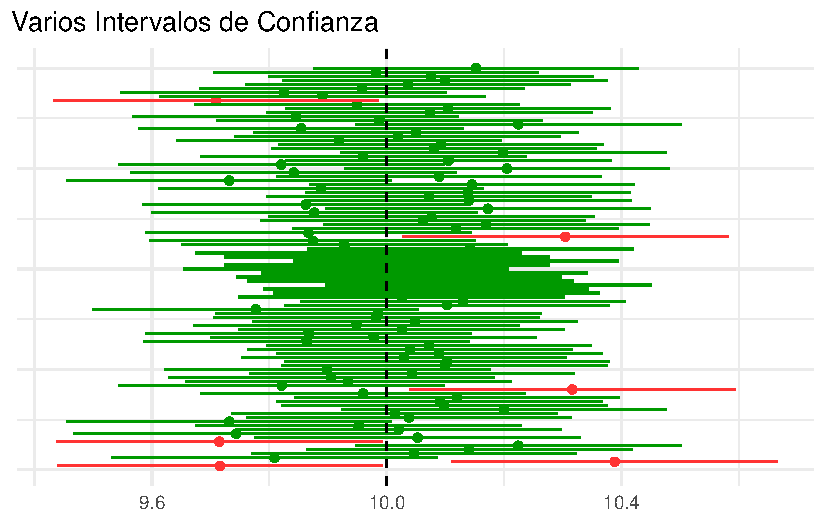
\includegraphics{para_files/figure-pdf/ic1-1.pdf}

}

\end{figure}

\begin{itemize}
\tightlist
\item
  ¿Cuántos intervalos de confianza, de entre los \(100\), contienen al
  verdadero valor del parámetro? Razona ese resultado.
\item
  ¿Cuándo se toma una única muestra, cómo podrías estar seguro de estar
  en uno de los intervalos de confianza que recoge el verdadero valor
  del parámetro?
\item
  ¿Cómo crees que afecta a la longitud del intervalo de confianza los
  siguientes aspectos:?

  \begin{itemize}
  \tightlist
  \item
    Tamaño muestral
  \item
    Nivel de confianza
  \end{itemize}
\end{itemize}

Discute estas cuestiones con tu profesor.

\end{tcolorbox}

\hypertarget{determinaciuxf3n-del-tamauxf1o-muestral}{%
\subsection{Determinación del tamaño
muestral}\label{determinaciuxf3n-del-tamauxf1o-muestral}}

Determinar el tamaño adecuado de una muestra es crucial en la inferencia
estadística, ya que un tamaño muestral adecuado garantiza que los
intervalos de confianza sean precisos y que las conclusiones obtenidas
sean representativas de la población. Las técnicas para determinar el
tamaño muestral están relacionadas directamente con los intervalos de
confianza y se basan en varios factores, entre los que se incluyen el
nivel de confianza deseado, la precisión (o margen de error) deseada y
la variabilidad esperada en la población.

Los factores clave para determinar el \textbf{tamaño muestral} son:

\begin{enumerate}
\def\labelenumi{\arabic{enumi}.}
\tightlist
\item
  \textbf{Nivel de Confianza} \(1-\alpha\):

  \begin{itemize}
  \tightlist
  \item
    El nivel de confianza indica el grado de certeza de que el intervalo
    de confianza contiene el parámetro poblacional. Tal y como hemos
    indicado anteriormente, niveles de confianza comunes son \(90\%\),
    \(95\%\) y \(99\%\). Un nivel de confianza más alto requiere una
    muestra más grande para asegurar la misma precisión.
  \end{itemize}
\item
  \textbf{Margen de Error (E)}:

  \begin{itemize}
  \tightlist
  \item
    El margen de error es la máxima diferencia tolerable entre la
    estimación muestral y el valor real del parámetro poblacional. Un
    margen de error más pequeño requiere una muestra más grande para
    asegurar una estimación precisa.
  \end{itemize}
\item
  \textbf{Variabilidad Poblacional} \(\sigma\):

  \begin{itemize}
  \tightlist
  \item
    La variabilidad en la población, medida por la desviación estándar,
    afecta directamente al tamaño muestral. Una mayor variabilidad
    requiere una muestra más grande para obtener una estimación precisa.
  \end{itemize}
\end{enumerate}

A continuación mostramos algunos ejemplos del cálculo del tamaño
muestral para diferentes situaciones.

\hypertarget{tamauxf1o-muestral-para-estimar-una-media-poblacional-de-una-normal}{%
\subsubsection{Tamaño muestral para estimar una media poblacional de una
Normal}\label{tamauxf1o-muestral-para-estimar-una-media-poblacional-de-una-normal}}

El tamaño muestral \(n\) necesario para estimar una media poblacional
con un margen de error \(E\) y un nivel de confianza \(1 - \alpha\) se
puede calcular usando la fórmula:

\[
n = \left( \frac{z_{\alpha/2} \cdot \sigma}{E} \right)^2
\]

donde: - \(z_{\alpha/2}\) es el valor crítico del estadístico \(z\)
correspondiente al nivel de confianza deseado. - \(\sigma\) es la
desviación estándar de la población (si es desconocida, se puede usar la
desviación estándar de la muestra \(s\)).

Efectivamente, teníamos que el intervalo de confianza para la media se
obtenía mediante la fórmula: \[
\left ( \bar{x} \pm z_{\alpha/2}\frac{\sigma}{\sqrt{n}} \right )
\] Y buscamos el \(n\) tal que la desviación respecto a la media sea
menor que \(E\), es decir: \[
 z_{\alpha/2}\frac{\sigma}{\sqrt{n}}  < E
\] \[
n >  \left ( \frac{z_{\alpha/2} \sigma}{\sqrt{n}} \right )^2
\]

\begin{tcolorbox}[enhanced jigsaw, arc=.35mm, breakable, coltitle=black, left=2mm, opacityback=0, bottomtitle=1mm, colbacktitle=quarto-callout-tip-color!10!white, title=\textcolor{quarto-callout-tip-color}{\faLightbulb}\hspace{0.5em}{Ejemplo. Tamaño muestral para la estimación de una Media}, titlerule=0mm, colback=white, colframe=quarto-callout-tip-color-frame, bottomrule=.15mm, rightrule=.15mm, opacitybacktitle=0.6, toptitle=1mm, toprule=.15mm, leftrule=.75mm]

Supongamos que deseamos estimar la media de una población con un nivel
de confianza del \(95\%\), un margen de error de \(5\) unidades y se
estima que la desviación estándar de la población es \(15\) unidades. El
valor crítico \(z_{\alpha/2}\) para un nivel de confianza del \(95\%\)
es aproximadamente \(1.96\).

\[
n = \left( \frac{1.96 \cdot 15}{5} \right)^2 = \left( \frac{29.4}{5} \right)^2 \approx 34.57
\]

Por lo tanto, necesitamos una muestra de al menos \(35\) individuos.

\end{tcolorbox}

\hypertarget{tamauxf1o-muestral-para-estimar-una-proporciuxf3n-poblacional}{%
\subsubsection{Tamaño muestral para estimar una proporción
poblacional}\label{tamauxf1o-muestral-para-estimar-una-proporciuxf3n-poblacional}}

El tamaño muestral \(n\) necesario para estimar una proporción
poblacional \(p\) con un margen de error \(E\) y un nivel de confianza
\(1 - \alpha\) se puede calcular usando la fórmula:

\[
n = \frac{z_{\alpha/2}^2 \cdot p \cdot (1 - p)}{E^2}
\]

donde: - \(p\) es la proporción esperada (si no se conoce, se usa
\(p = 0.5\) para maximizar el tamaño muestral). - \(z_{\alpha/2}\) es el
valor crítico del estadístico \(z\) correspondiente al nivel de
confianza deseado.

\begin{tcolorbox}[enhanced jigsaw, arc=.35mm, breakable, coltitle=black, left=2mm, opacityback=0, bottomtitle=1mm, colbacktitle=quarto-callout-tip-color!10!white, title=\textcolor{quarto-callout-tip-color}{\faLightbulb}\hspace{0.5em}{Ejemplo. Tamaño muestral para la estimación de una proporción}, titlerule=0mm, colback=white, colframe=quarto-callout-tip-color-frame, bottomrule=.15mm, rightrule=.15mm, opacitybacktitle=0.6, toptitle=1mm, toprule=.15mm, leftrule=.75mm]

Supongamos que deseamos estimar la proporción de personas que aprueban
una nueva ley con un nivel de confianza del \(95\%\), un margen de error
del \(3\%\) \((0.03)\) y se estima que la proporción esperada es
\(p = 0.5\). El valor crítico \(z_{\alpha/2}\) para un nivel de
confianza del \(95\%\) es aproximadamente \(1.96\).

\[
n = \frac{1.96^2 \cdot 0.5 \cdot (1 - 0.5)}{0.03^2} = \frac{3.8416 \cdot 0.25}{0.0009} = \frac{0.9604}{0.0009} \approx 1067.11
\]

Por lo tanto, necesitamos una muestra de al menos \(1068\) individuos.

\end{tcolorbox}

\hypertarget{contraste-de-hipuxf3tesis-1}{%
\section{Contraste de hipótesis}\label{contraste-de-hipuxf3tesis-1}}

Los contrastes de hipótesis son una herramienta fundamental en la
inferencia estadística utilizada para tomar decisiones basadas en datos
muestrales. Permiten evaluar si los datos disponibles proporcionan
suficiente evidencia en contra de una hipótesis previamente establecida
sobre una población.

El contraste de hipótesis es un proceso estructurado para evaluar
afirmaciones sobre parámetros poblacionales utilizando datos muestrales.
Mediante la formulación de hipótesis, selección de niveles de
significancia, elección de estadísticas de prueba y evaluación del valor
p, podemos tomar decisiones informadas y cuantitativamente justificadas.
Este enfoque es fundamental en muchas áreas de investigación y análisis
de datos, proporcionando un marco riguroso para la inferencia
estadística.

\hypertarget{conceptos-buxe1sicos-1}{%
\subsection{Conceptos Básicos}\label{conceptos-buxe1sicos-1}}

\textbf{Hipótesis Nula} \((H_0)\):

\begin{itemize}
\item
  La hipótesis nula es una afirmación sobre un parámetro poblacional que
  se asume verdadera hasta que se presente suficiente evidencia en
  contra. Se asume inicialmente que la hipótesis nula es correcta
  (semejante a suponer inocencia a menos que se pruebe la culpa).
  Habitualmente corresponde al estatus quo. Esto es, generalmente, la
  hipótesis nula representa un estado de ``no efecto'' o ``no
  diferencia''.

  \begin{itemize}
  \tightlist
  \item
    Ejemplo: \((H_0: \mu = 50)\) (la media poblacional es \(50\)). En
    este ejemplo, la idea fundamental del contraste sería toma una
    muestra aleatoria simple de la población, estudiar su media, y ver
    si hay evidencia suficiente como para rechazar la hipótesis nula
    establecida. La probabilidad de que la media sea \emph{exactamente}
    igual a \(50\) en la muestra es muy baja. Es decir, probablemente
    \(\bar{\mathbf{x}} \neq 50\). Sin embargo, lo importante para
    rechazar la hipótesis nula es si la diferencia encontrada entre la
    media muestral y \(50\) es tan grande como para rechazar que podría
    ser \(50\).
  \end{itemize}
\end{itemize}

\textbf{Hipótesis Alternativa} \((H_1)\):

\begin{itemize}
\item
  La hipótesis alternativa es una afirmación que contrasta con la
  hipótesis nula y representa el efecto o diferencia que se desea
  detectar.

  \begin{itemize}
  \tightlist
  \item
    Ejemplo: \((H_1: \mu \neq 50)\) (la media poblacional no es 50).
  \item
    Ejemplo: \((H_1: \mu \geq 50)\) (la media poblacional es mayor o
    igual que 50).
  \end{itemize}
\end{itemize}

\begin{tcolorbox}[enhanced jigsaw, arc=.35mm, breakable, coltitle=black, left=2mm, opacityback=0, bottomtitle=1mm, colbacktitle=quarto-callout-tip-color!10!white, title=\textcolor{quarto-callout-tip-color}{\faLightbulb}\hspace{0.5em}{Ejemplo \(H_0\) vs \(H_1\). Media poblacional}, titlerule=0mm, colback=white, colframe=quarto-callout-tip-color-frame, bottomrule=.15mm, rightrule=.15mm, opacitybacktitle=0.6, toptitle=1mm, toprule=.15mm, leftrule=.75mm]

Supongamos que una empresa de educación en línea afirma que sus
estudiantes pasan en promedio al menos \(4\) horas diarias estudiando en
su plataforma. Queremos comprobar si esta afirmación es cierta
basándonos en una muestra de estudiantes.

\begin{itemize}
\item
  La hipótesis nula es la afirmación que queremos poner a prueba y que
  asumimos verdadera inicialmente. En este caso, la hipótesis nula es
  que la media del tiempo de estudio diario es de \(4\) horas. \[
   H_0: \mu \geq 4 \text{ horas}
   \]
\item
  La hipótesis alternativa es lo que queremos demostrar y se contrapone
  a la hipótesis nula. En este caso, queremos ver si el tiempo de
  estudio diario es menor de \(4\) horas. Fíjate que la empresa podría
  estar ``inflando'' sus resultados y lo ``intersante'' en este caso es
  ``demostrar'' que realmente los alumnos pasan menos tiempo en la
  plataforma. \[
   H_1: \mu < 4 \text{ horas}
  \]
\end{itemize}

\end{tcolorbox}

\begin{tcolorbox}[enhanced jigsaw, arc=.35mm, breakable, coltitle=black, left=2mm, opacityback=0, bottomtitle=1mm, colbacktitle=quarto-callout-tip-color!10!white, title=\textcolor{quarto-callout-tip-color}{\faLightbulb}\hspace{0.5em}{Ejemplo \(H_0\) vs \(H_1\). Proporción poblacional}, titlerule=0mm, colback=white, colframe=quarto-callout-tip-color-frame, bottomrule=.15mm, rightrule=.15mm, opacitybacktitle=0.6, toptitle=1mm, toprule=.15mm, leftrule=.75mm]

Supongamos que el rectorado de la URJC afirma que menos del \(20\%\) de
los estudiantes de sus grados, fuman. Queremos verificar si la
proporción de fumadores es mayor al \(20\%\).

\begin{itemize}
\item
  La hipótesis nula es la afirmación que queremos poner a prueba y que
  asumimos verdadera inicialmente. En este caso, la hipótesis nula es
  que la proporción de fumadores es menor o igual al \(20\%\). \[
   H_0: p \leq 0.20
  \]
\item
  La hipótesis alternativa es lo que queremos demostrar y se contrapone
  a la hipótesis nula. En este caso, queremos ver si la proporción de
  fumadores es mayor al \(20\%\). \[
   H_1: p > 0.20
  \]
\end{itemize}

\end{tcolorbox}

\hypertarget{pasos-en-un-contraste-de-hipuxf3tesis}{%
\subsection{Pasos en un Contraste de
Hipótesis}\label{pasos-en-un-contraste-de-hipuxf3tesis}}

\begin{enumerate}
\def\labelenumi{\arabic{enumi}.}
\tightlist
\item
  \textbf{Formular las hipótesis}:

  \begin{itemize}
  \tightlist
  \item
    Definir \(H_0\) y \(H_1\) claramente.
  \end{itemize}
\item
  \textbf{Seleccionar el nivel de significatividad estadística}
  \((\alpha)\):

  \begin{itemize}
  \tightlist
  \item
    El nivel de significatividad estadística es la probabilidad de
    rechazar \(H_0\) cuando es verdadera. Comúnmente, se utilizan
    \(\alpha = 0.05\), \(\alpha = 0.01\), o \(\alpha = 0.10\).
  \end{itemize}
\item
  \textbf{Elegir el estadístico de prueba}:

  \begin{itemize}
  \tightlist
  \item
    Seleccionar un estadístico que siga una distribución conocida bajo
    \(H_0\) (por ejemplo, la distribución Normal, t de Student o
    Chi-cuadrado).
  \end{itemize}
\item
  \textbf{Calcular el} \(p-valor\):

  \begin{itemize}
  \tightlist
  \item
    El \(p-valor\) es la probabilidad de observar un valor tan extremo o
    más extremo que el observado, bajo la suposición de que \(H_0\) es
    verdadera. Después volveremos sobre este valor.
  \end{itemize}
\item
  \textbf{Tomar una decisión}:

  \begin{itemize}
  \tightlist
  \item
    La regla de decisión de un contraste de hipótesis se basa en la
    ``distancia'' entre los datos muestrales y los valores esperados si
    \(H_0\) es cierta. Esta distancia se calcula a partir de un
    estadístico del contraste y se considera ``grande'' o no, en base a
    la distribución del mismo y a la probabilidad de observar
    realizaciones ``más extremas'' de dicho estadístico. Para tomar la
    decisión, comparamos el valor p con \(\alpha\):
  \item
    Si \(p-valor \leq \alpha\), se rechaza \(H_0\). Hay suficiente
    evidencia en la muestra como para rechazar la hipótesis nula. El
    valor del parámetro establecido en \(H_0\) es poco creíble dada la
    muestra observada.
  \item
    Si \(p-valor > \alpha\), no se rechaza \(H_0\). \textbf{Muy
    importante}: esto no significa que la hipótesis nula sea cierta. La
    interpretación es que no existe, en la muestra que hemos observado,
    suficiente evidencia en contra de la hipótesis nula como para
    recharzarla.
  \end{itemize}
\end{enumerate}

Tenemos por tanto que el \(p-valor\) es una medida que nos dice cuán
probable sería obtener nuestros datos observados si la hipótesis nula
fuera verdadera. En otras palabras, mide la evidencia en contra \(H_0\).
Si el \(p-valor\) es pequeño (generalmente menor que \(0.05\)), tenemos
razones para rechazar \(H_0\). Si es grande, no tenemos suficiente
evidencia para rechazarla.

\begin{tcolorbox}[enhanced jigsaw, arc=.35mm, breakable, coltitle=black, left=2mm, opacityback=0, bottomtitle=1mm, colbacktitle=quarto-callout-tip-color!10!white, title=\textcolor{quarto-callout-tip-color}{\faLightbulb}\hspace{0.5em}{Ejemplo Práctico. Contraste de Hipótesis}, titlerule=0mm, colback=white, colframe=quarto-callout-tip-color-frame, bottomrule=.15mm, rightrule=.15mm, opacitybacktitle=0.6, toptitle=1mm, toprule=.15mm, leftrule=.75mm]

Supongamos que una empresa afirma que el tiempo promedio de espera en su
servicio al cliente es de \(10\) minutos. Queremos probar esta
afirmación con una muestra de \(30\) clientes que tienen un tiempo
promedio de espera de \(12\) minutos y una desviación estándar de \(3\)
minutos.

Formulamos las hipótesis: - \(H_0: \mu = 10\) - \(H_1: \mu \neq 10\)

Seleccionamos el nivel de significancia estadística deseado:
\(\alpha = 0.05\).

Elegimos el estadístico de prueba: usamos una prueba \(t\) (dado que la
muestra es pequeña y no conocemos la desviación estándar poblacional) y
calculamos su valor:

\[
   t = \frac{\bar{x} - \mu_0}{s / \sqrt{n}} = \frac{12 - 10}{3 / \sqrt{30}} \approx \frac{2}{0.5477} \approx 3.65
\]

A continuación, obtenemos el \(p-valor\) correspondiente al estadístico
para la distribución \(t\) de Studento con \(29\) grados de libertad.
Para \(t = 3.65\), el \(p-valor\) es menor que \(0.001\).

Dado que \(p < 0.05\), rechazamos la hipótesis nula \(H_0\). Podemos
afirmar que los resultados muestrales son ``demasiado extraños'' para
aceptar la hipótesis nula.

\end{tcolorbox}

\hypertarget{errores-tipo-i-y-tipo-ii.-potencia}{%
\subsection{Errores tipo I y tipo II.
Potencia}\label{errores-tipo-i-y-tipo-ii.-potencia}}

Como hemos visto, una vez especificadas las hipótesis nula y alternativa
y recogida la información muestral, se toma una decisióon sobre la
hipótesis nula (rechazar o no rechazar H0). Sin embargo, Existe la
posibilidad de llegar a una conclusión equivocada, porque solo se
dispone de una muestra aleatoria y no se puede tener la certeza de que
\(H_0\) sea correcta o no.

En la inferencia estadística, cuando realizamos un contraste de
hipótesis, hay dos tipos de errores que pueden ocurrir: el \textbf{error
de tipo I o} \(\alpha\) y el \textbf{error de tipo II on} \(\beta\).
Entender estos errores es fundamental para interpretar correctamente los
resultados de cualquier prueba estadística. El balance entre \(\alpha\)
y \(\beta\), así como el tamaño de la muestra, juegan un papel
importante en la fiabilidad de los resultados obtenidos.

\hypertarget{error-de-tipo-i-alpha}{%
\subsubsection{\texorpdfstring{Error de Tipo I
\((\alpha)\)}{Error de Tipo I (\textbackslash alpha)}}\label{error-de-tipo-i-alpha}}

El error de tipo I ocurre cuando rechazamos la hipótesis nula \(H_0\)
siendo esta verdadera. En otras palabras, concluimos que hay un efecto o
una diferencia cuando, en realidad, no la hay. El nivel de significancia
\(\alpha\) es la probabilidad de cometer un error de tipo I.

\[
\alpha=P(\text{rechazar } H_0 \text{ | } H_0 \text{ es correcta})
\]

Recuerda que establecemos de antemano esta valor, comúnmente \(0.05\),
\(0.01\) o \(0.10\). Si el \(p-valor\) de nuestra prueba es menor o
igual a \(\alpha\), rechazamos \(H_0\).

Así, por ejemplo, Si \(\alpha = 0.05\), esto significa que estamos
dispuestos a aceptar un \(5\%\) de probabilidad de rechazar \(H_0\)
cuando es verdadera.

::: \{callout-caution title=``Atención''\} ¿Qué relación existe entre el
error de tipo I y el \(\%\) de un IC? :::

\hypertarget{error-de-tipo-ii-beta}{%
\subsubsection{\texorpdfstring{Error de Tipo II
\((\beta)\)}{Error de Tipo II (\textbackslash beta)}}\label{error-de-tipo-ii-beta}}

El error de tipo II ocurre cuando no rechazamos la hipótesis nula
\(H_0\) siendo esta falsa. En otras palabras, concluimos que no hay un
efecto o una diferencia cuando, en realidad, sí la hay.

\[
\beta=P(\text{No rechazar } H_0 \text{ | } H_0 \text{ es incorrecta})
\]

\textbf{Potencia del test}: La potencia de una prueba estadística es la
probabilidad de rechazar \(H_0\) cuando \(H_0\) es falsa. Se calcula
como \(1 - \beta\). Una alta potencia es deseable ya que indica una
mayor probabilidad de detectar un efecto o diferencia cuando realmente
existe.

\[
Potencia=1-\beta=P(\text{Rechazar } H_0 \text{ | } H_1 \text{ es correcta})
\]

Así, por ejemplo, si \(\beta = 0.20\), esto significa que hay un
\(20\%\) de probabilidad de no rechazar \(H_0\) cuando es falsa. La
potencia de la prueba sería \(0.80\) (o del \(80\%\)). La probabilidad
de detectar un efecto cuando relamente existe es del \(80\%\)

\begin{tcolorbox}[enhanced jigsaw, arc=.35mm, breakable, coltitle=black, left=2mm, opacityback=0, bottomtitle=1mm, colbacktitle=quarto-callout-tip-color!10!white, title=\textcolor{quarto-callout-tip-color}{\faLightbulb}\hspace{0.5em}{Ejemplo Práctico. Errores Tipo I y II}, titlerule=0mm, colback=white, colframe=quarto-callout-tip-color-frame, bottomrule=.15mm, rightrule=.15mm, opacitybacktitle=0.6, toptitle=1mm, toprule=.15mm, leftrule=.75mm]

Supongamos que estamos evaluando la efectividad de un nuevo medicamento.

\begin{itemize}
\tightlist
\item
  Hipótesis Nula \(H_0\): El medicamento no tiene efecto \((\mu = 0)\).
\item
  Hipótesis Alternativa \(H_1\): El medicamento tiene un efecto
  \((\mu \neq 0)\).
\end{itemize}

\begin{enumerate}
\def\labelenumi{\arabic{enumi}.}
\item
  Error de Tipo I: Si el medicamento no tiene ningún efecto pero el
  estudio concluye que sí lo tiene, hemos cometido un error de tipo I.
  Esto podría llevar a la aprobación y uso de un medicamento ineficaz.
\item
  Error de Tipo II: Si el medicamento tiene un efecto, pero el estudio
  concluye que no lo tiene, hemos cometido un error de tipo II. Esto
  podría llevar a la no aprobación de un medicamento potencialmente
  beneficioso.
\end{enumerate}

\end{tcolorbox}

\hypertarget{relaciuxf3n-entre-errores-de-tipo-i-y-ii}{%
\subsubsection{Relación entre errores de tipo I y
II}\label{relaciuxf3n-entre-errores-de-tipo-i-y-ii}}

\begin{itemize}
\tightlist
\item
  \textbf{Inversamente proporcionales}: Reducir \(\alpha\) (haciendo la
  prueba más conservadora y menos propensa a rechazar \(H_0\)
  generalmente aumenta \(\beta\) (haciendo la prueba más propensa a no
  detectar un efecto cuando realmente existe), y viceversa. Fíjate que
  los errores de Tipo I y de Tipo II no se pueden comenter
  simultáneamente:

  \begin{itemize}
  \tightlist
  \item
    El error de Tipo I solo puede darse si \(H_0\) es correcta.
  \item
    El error de Tipo II solo puede darse si \(H_0\) es incorrecta.
  \end{itemize}
\item
  \textbf{Tamaño de la muestra}: Aumentar el tamaño de la muestra puede
  reducir ambos tipos de errores, incrementando la precisión de la
  prueba.
\end{itemize}

La siguiente tabla refleja la relación entre los dos tipos de errores en
relación con la decisión del contraste y la verdadera situación en la
población:

\begin{longtable}[]{@{}
  >{\raggedright\arraybackslash}p{(\columnwidth - 4\tabcolsep) * \real{0.2603}}
  >{\raggedright\arraybackslash}p{(\columnwidth - 4\tabcolsep) * \real{0.3425}}
  >{\raggedright\arraybackslash}p{(\columnwidth - 4\tabcolsep) * \real{0.3973}}@{}}
\toprule\noalign{}
\begin{minipage}[b]{\linewidth}\raggedright
\end{minipage} & \begin{minipage}[b]{\linewidth}\raggedright
\textbf{Verdadera situación}
\end{minipage} & \begin{minipage}[b]{\linewidth}\raggedright
\end{minipage} \\
\midrule\noalign{}
\endhead
\bottomrule\noalign{}
\endlastfoot
\textbf{Decisión} & \(H_0\) correcta & \(H_0\) incorrecta \\
No rechazar \(H_0\) & Sin error (\(1-\alpha\)) & Error de Tipo II
(\(\beta\)) \\
Rechazar \(H_0\) & Error de Tipo I (\(\alpha\)) & Sin error
(\(1-\beta\)=potencia) \\
\end{longtable}

Es importante notar que, si todo lo demás no cambia, entonces la
potencia del contraste disminuye cuando:

\begin{itemize}
\tightlist
\item
  La diferencia entre el valor supuesto para el parámetro y el valor
  real disminuye.
\item
  La variabilidad de la población aumenta.
\item
  El tamaño muestra disminuye.
\end{itemize}

\begin{tcolorbox}[enhanced jigsaw, arc=.35mm, breakable, coltitle=black, left=2mm, opacityback=0, bottomtitle=1mm, colbacktitle=quarto-callout-tip-color!10!white, title=\textcolor{quarto-callout-tip-color}{\faLightbulb}\hspace{0.5em}{Ejemplo Práctico. Errores Tipo I y II}, titlerule=0mm, colback=white, colframe=quarto-callout-tip-color-frame, bottomrule=.15mm, rightrule=.15mm, opacitybacktitle=0.6, toptitle=1mm, toprule=.15mm, leftrule=.75mm]

Los errores de tipo I y tipo II son inversamente proporcionales. Al
disminuir la probabilidad de cometer un error de tipo I (haciendo la
prueba más conservadora), aumentamos la probabilidad de cometer un error
de tipo II (haciendo la prueba menos sensible), y viceversa.

Supongamos que estamos evaluando la efectividad de un nuevo medicamento
para reducir la presión arterial. Queremos probar la siguiente
hipótesis:

\begin{itemize}
\tightlist
\item
  Hipótesis Nula \((H_0)\): El nuevo medicamento no reduce la presión
  arterial (\(\mu = 0\)).
\item
  Hipótesis Alternativa \((H_1)\): El nuevo medicamento reduce la
  presión arterial \((\mu \neq 0)\).
\end{itemize}

Inicialmente fijamos el nivel de significancia (\(\alpha\)) en \(0.05\).
Consideramos un tamaño de muestra inicial de \(100\) pacientes.

En este caso el error de Tipo I, significa que estamos dispuestos a
aceptar un \(5\%\) de probabilidad de concluir que el medicamento es
efectivo cuando en realidad no lo es.

La probabilidad de error de Tipo II (\(\beta\)) y, por tanto, la
pontencia del contraste depende de varios factores, incluidos el tamaño
del efecto, el tamaño de la muestra y el nivel de significancia.

\textbf{Caso 1: (}\(\alpha = 0.05\))

En este caso somos bastante conservadores con el riesgo de falso
positivo. Supongamos que el poder estadístico de la prueba con
\((\alpha = 0.05)\) y una muestra de \(100\) es \(0.80\), lo que
significa que (\(\beta = 0.20\)).

\textbf{Caso 2: (}\(\alpha = 0.01\))

Ahora somos más conservadores, reduciendo la probabilidad de cometer un
error de tipo I. Al ser más conservadores y reducir (\(\alpha\)), la
prueba se vuelve menos sensible a detectar el efecto real. Esto aumenta
la probabilidad de cometer un error de tipo II, por ejemplo, supongamos
que (\(\beta\)) aumenta a \(0.30\). Se reduce la potencia del contraste.

\textbf{Caso 3: (}\(\alpha = 0.10\))

Ahora somos menos conservadores, aumentando la probabilidad de cometer
un error de tipo I. Al ser menos conservadores y aumentar (\(\alpha\)),
la prueba se vuelve más sensible a detectar el efecto real. Esto
disminuye la probabilidad de cometer un error de tipo II, por ejemplo,
supongamos que (\(\beta\)) disminuye a 0.10 y, por tanto, aumenta la
potencia del contraste.

En resumen:

\begin{longtable}[]{@{}ccc@{}}
\toprule\noalign{}
\(\alpha\) & \(\beta\) & Potencia (\(1-\beta\)) \\
\midrule\noalign{}
\endhead
\bottomrule\noalign{}
\endlastfoot
0.05 & 0.20 & 0.80 \\
0.01 & 0.30 & 0.70 \\
0.10 & 0.10 & 0.90 \\
\end{longtable}

y como conclusión

\begin{itemize}
\tightlist
\item
  \textbf{Caso 1 (}\(\alpha = 0.05\)): Balance estándar entre el riesgo
  de falso positivo y falso negativo.
\item
  \textbf{Caso 2 (}\(\alpha = 0.01\)): Reducimos el riesgo de falso
  positivo (\(\alpha\)), pero aumentamos el riesgo de falso negativo
  ((\beta)).
\item
  \textbf{Caso 3 (}\(\alpha = 0.10\)): Aumentamos el riesgo de falso
  positivo (\(\alpha\)), pero reducimos el riesgo de falso negativo
  (\(\beta\)).
\end{itemize}

\end{tcolorbox}

\hypertarget{contraste-para-la-media-de-una-poblaciuxf3n-normal-con-varianza-conocida}{%
\subsection{Contraste para la media de una población normal con varianza
conocida}\label{contraste-para-la-media-de-una-poblaciuxf3n-normal-con-varianza-conocida}}

El contraste para la media de una población normal con varianza conocida
es un procedimiento estadístico utilizado para determinar si la media de
una población difiere de un valor específico (hipótesis nula). Sin
embargo, como hemos indicado anteriormente, es poco realista pensar que
conocemos la varianza de una variable aleatoria en la población.

El parámetr de estudio es la media d ela variable aleatoria:

\[ X \sim N(\mu,\sigma^2) \]

En primer lugar fijamos las hipótesis:

\begin{itemize}
\tightlist
\item
  \(H_0\): \(\mu = \mu_0\) (La media de la población es igual a
  \(\mu_0\))
\end{itemize}

Tenemos varias opciones para la hipótesis alternativa:

\begin{itemize}
\tightlist
\item
  \(H_1\): \(\mu \neq \mu_0\) (Contraste bilateral)
\item
  \(H_1\): \(\mu > \mu_0\) (Contraste unilateral derecho)
\item
  \(H_1\): \(\mu < \mu_0\) (Contraste unilateral izquierdo)
\end{itemize}

Debemos fijar el nivel de el nivel de significación (\(\alpha\)).
Recordemos, es la probabilidad de rechazar la hipótesis nula cuando esta
es verdadera.

El estadístico de prueba se calcula utilizando la distribución Normal
estándar (\(Z\)), dado que la varianza (\(\sigma^2\)) es conocida. La
fórmula para el estadístico de prueba es:

\[ Z = \frac{\bar{\mathbf{X}} - \mu_0}{\sigma/\sqrt{n}} \sim N(0,1) \]

Donde \(\bar{\mathbf{X}}\) es la media poblacional. Calculamos el valor
observado del estadístico:
\[ z = \frac{\bar{\mathbf{x}} - \mu_0}{\sigma/\sqrt{n}} \] donde
\(\bar{\mathbf{x}}\) es la media muestral.

Después calculamos el \(p-valor\) como sigue:

\begin{itemize}
\item
  Contraste bilateral:\(p-valor=P(|Z|\geq z)\)
\item
  Contraste unilateral derecho:\(p-valor=P(Z\geq z)\)
\item
  Contraste unilateral izquierdo:\(p-valor=P(Z\leq z)\)
\end{itemize}

Si esta probabilidad es menor o igual que el valor de referencia
\(\alpha\) entonces, rechazamos la hipótesis nula en favor de la
alternativa.

Otra forma práctica de plantear el contraste de hipótesis es
determinando el Rechazo de \(H_0\) Para ello, debemos comparar el valor
del estadístico \(Z\) con los valores críticos de la distribución Normal
estándar.

\begin{itemize}
\tightlist
\item
  Para un contraste bilateral (dos colas):

  \begin{itemize}
  \tightlist
  \item
    Rechaza \(H_0\) si \(|z| > z_{\alpha/2}\).
  \end{itemize}
\item
  Para un contraste unilateral derecho (una cola):

  \begin{itemize}
  \tightlist
  \item
    Rechaza \(H_0\) si \(z > z_{\alpha}\).
  \end{itemize}
\item
  Para un contraste unilateral izquierdo (una cola):

  \begin{itemize}
  \tightlist
  \item
    Rechaza \(H_0\) si \(z < -z_{\alpha}\).
  \end{itemize}
\end{itemize}

Aquí, \(z_{\alpha}\) y \(z_{\alpha/2}\) son los valores críticos de la
distribución Normal estándar correspondientes al nivel de significación
\(\alpha\).

Es decir, decidimos si rechazamos o no la hipótesis nula del siguiente
modo:

\begin{itemize}
\tightlist
\item
  Si el valor del estadístico de prueba está en la región crítica,
  rechaza (H\_0).
\item
  Si el valor del estadístico de prueba no está en la región crítica, no
  rechaces (H\_0).
\end{itemize}

\begin{tcolorbox}[enhanced jigsaw, arc=.35mm, breakable, coltitle=black, left=2mm, opacityback=0, bottomtitle=1mm, colbacktitle=quarto-callout-tip-color!10!white, title=\textcolor{quarto-callout-tip-color}{\faLightbulb}\hspace{0.5em}{Ejemplo Práctico. Contraste de hipótesis media normal, varianza conocida}, titlerule=0mm, colback=white, colframe=quarto-callout-tip-color-frame, bottomrule=.15mm, rightrule=.15mm, opacitybacktitle=0.6, toptitle=1mm, toprule=.15mm, leftrule=.75mm]

Supón que queremos probar si la edad media de los profesores de la URJC
es igual a \(50\) años con una desviación estándar conocida de \(10\)
años, y tienes una muestra de \(36\) observaciones con una media
muestral de \(52\).

Formulamos las hipótesis:

\begin{itemize}
\tightlist
\item
  \(H_0\): \(\mu = 50\)
\item
  \(H_1\): \(\mu \neq 50\)
\end{itemize}

Fijamos el nivel de significación: \(\alpha = 0.05\).

Calculamos el estadístico de prueba:
\[ z = \frac{52 - 50}{10/\sqrt{36}}  \approx 1.20 \]

Para \(\alpha = 0.05\) en un contraste bilateral, los valores críticos
son \(z_{0.05/2}=\pm 1.96\). Como \(|1.20| < 1.96\), no tenemos
evidencia en la muestra como para rechazar \(H_0\).

Si hubiéramos calculado el \(p-valor\):
\[p-valor=P(|Z| \geq 1.20)=2*P(Z \geq 1.20)=2*0.115\approx0.23\] Como el
\(p-valor\) es mayor que el nivel de significatividad estadística, no
podemos rechazar la hipótesis nula en favor de la alternativa.

\end{tcolorbox}

\hypertarget{contraste-para-la-media-de-una-poblaciuxf3n-normal-con-varianza-desconocida}{%
\subsection{Contraste para la media de una población normal con varianza
desconocida}\label{contraste-para-la-media-de-una-poblaciuxf3n-normal-con-varianza-desconocida}}

El contraste de hipótesis para la media de una población normal con
varianza desconocida es similar al caso con varianza conocida, pero
utilizamos la distribución \(t\) de Student en lugar de la distribución
Normal estándar.

En este caso, el cuando la varianza poblacional es desconocida, se
utiliza la desviación estándar muestral (\(s\)) y el estadístico de
prueba se basa en la distribución \(t\) de Student con (\(n - 1\))
grados de libertad. La fórmula es:

\[ T=\frac{\bar{X} - \mu_0}{s/\sqrt{n}} \]

Donde \(\bar{\mathbf{X}}\) es la media poblacional. Calculamos el valor
observado del estadístico: \[ t = \frac{\bar{x} - \mu_0}{s/\sqrt{n}}  \]

El p-valor es la probabilidad de obtener un valor del estadístico de
prueba al menos tan extremo como el observado, bajo la suposición de que
\(H_0\) es verdadera. Dependiendo del tipo de contraste, el p-valor se
calcula de diferentes formas:

\begin{itemize}
\tightlist
\item
  Para un contraste bilateral:

  \begin{itemize}
  \tightlist
  \item
    p-valor = \(2 \cdot P(T_{n-1} > |t|)\)
  \end{itemize}
\item
  Para un contraste unilateral derecho:

  \begin{itemize}
  \tightlist
  \item
    p-valor = \(P(T_{n-1} > t)\)
  \end{itemize}
\item
  Para un contraste unilateral izquierdo:

  \begin{itemize}
  \tightlist
  \item
    p-valor = \(P(T_{n-1} < t)\)
  \end{itemize}
\end{itemize}

Aquí, \(T_{n-1}\) es una variable aleatoria con una distribución \(t\)
de Student con \(n - 1\) grados de libertad.

La decisión asociada al contraste es:

\begin{itemize}
\tightlist
\item
  Si el \(p-valor \leq \alpha\), rechazar \(H_0\).
\item
  Si el \(p-valor > \alpha\), no rechazar \(H_0\).
\end{itemize}

\begin{tcolorbox}[enhanced jigsaw, arc=.35mm, breakable, coltitle=black, left=2mm, opacityback=0, bottomtitle=1mm, colbacktitle=quarto-callout-tip-color!10!white, title=\textcolor{quarto-callout-tip-color}{\faLightbulb}\hspace{0.5em}{Ejemplo Práctico. Contraste de hipótesis media normal, varianza
desconocida}, titlerule=0mm, colback=white, colframe=quarto-callout-tip-color-frame, bottomrule=.15mm, rightrule=.15mm, opacitybacktitle=0.6, toptitle=1mm, toprule=.15mm, leftrule=.75mm]

Supón que una empresa quiere verificar si el tiempo promedio de entrega
de sus pedidos es mayor de \(30\) minutos. Toma una muestra aleatoria de
\(16\) entregas y encuentra que el tiempo promedio de entrega es de
\(32\) minutos con una desviación estándar muestral de \(4\) minutos.
Realiza un contraste de hipótesis con un nivel de significación del
\(0.05\) para ver si el tiempo promedio de entrega es mayor de \(30\)
minutos.

En primer lugar establecemos las hipótesis: - \(H_0\): \$\mu = 30 (El
tiempo promedio de entrega es de 30 minutos) - \(H_1\):
\$\mu \textgreater{} 30 (El tiempo promedio de entrega es mayor de 30
minutos)

Calculamos el estadístico de Prueba
\[ t = \frac{\bar{X} - \mu_0}{s/\sqrt{n}} = \frac{32 - 30}{4/\sqrt{16}} = \frac{2}{1} = 2.00 \]

Estamos ante un contraste unilateral derecho con \(n - 1 = 16 - 1 = 15\)
grados de libertad. El \(p-valor\) es:
\[P(T_{15} > 2.00) \approx 0.031\]

Como el \(p-valor\) es menor que el grado de significatividad
estadística \(0.05\), entonces podemos rechazar la hipótesis nula en
favor de la alternativa. Hay suficiente evidencia para rechazar la
hipótesis nula y concluir que el tiempo promedio de entrega es mayor de
\(30\) minutos con un nivel de significación del \(5\%\).

\end{tcolorbox}

\hypertarget{contraste-de-hipuxf3tesis-para-la-igualdad-de-medias-de-dos-muestras-independientes}{%
\subsection{Contraste de hipótesis para la igualdad de medias de dos
muestras
independientes}\label{contraste-de-hipuxf3tesis-para-la-igualdad-de-medias-de-dos-muestras-independientes}}

Cuando se desea comparar las medias de dos muestras independientes
asumiendo que los datos siguen una distribución normal, se puede usar el
contraste de hipótesis paramétrico conocido como la prueba \(t\) de
Student para muestras independientes. Este método es robusto y se basa
en suposiciones claras acerca de la normalidad de las distribuciones
subyacentes.

\textbf{Suposiciones:}

\begin{itemize}
\tightlist
\item
  Las dos muestras son independientes.
\item
  Los datos de cada muestra se distribuyen normalmente. Si las muestras
  son suficientemente grandes, se puede invocar el \emph{Teorema Central
  del Límite}, que establece que la distribución de la media muestral se
  aproxima a una distribución normal independientemente de la forma de
  la distribución original.
\item
  Las varianzas poblacionales son desconocidas, pero se pueden asumir
  iguales para una versión específica del test t (si esta suposición es
  razonable).
\end{itemize}

Supongamos m.a.s. independientes con medias, desviaciones típicas y
tamaño muestral igual a:
\(\bar{\mathbf{x}}_1\),\(\bar{\mathbf{x}}_2\),\(s_1^2\),\(s_2^2\),\(n_1\),y
\(n_2\), respectivamente.

Formulamos las hipótesis:

\begin{itemize}
\tightlist
\item
  \textbf{Hipótesis nula (}\(H_0\)): Las medias de las dos poblaciones
  son iguales (\(\mu_1=\mu_2\)).
\item
  \textbf{Hipótesis alternativa (}\(H_1\)): Las medias de las dos
  poblaciones son diferentes (\(mu_1 \neq \mu_2\)).
\end{itemize}

Consideramos un nivel de significancia estadística \(\alpha\).
Típicamente \(\alpha=0.05\).

Calculamos el estadístico muestras, en este caso: \[
t = \frac{\bar{\mathbf{x}}_1-\bar{\mathbf{x}}_2}{SE}
\] donde: \[
SE = \sqrt{S^2_p \left( \frac{1}{n₁} + \frac{1}{n₂} \right)}
\] siendo \(S_p\) la desviación típica combinada: \[
S^2_p= \frac{(n_1 - 1)s_1^2 + (n_2 - 1)s_2^2}{n_1 + n_2 - 2}
\]

Para un nivel de significancia \(\alpha= 0.05\) y grados de libertad
\(df = n_1+n_2-2\), buscamos el valor crítico \(t\) para la distribución
\(t\) de Student para una prueba de dos colas.

Comparamos el valor del estadístico \(t\) calculado con el valor
crítico:

\begin{itemize}
\tightlist
\item
  Si \(|t| > T_{df,1-\alpha/2}\), rechazamos \(H_0\).
\item
  Si \(|t| \leq T_{df,1-\alpha/2}\), no rechazamos \(H_0\).
\end{itemize}

\begin{tcolorbox}[enhanced jigsaw, arc=.35mm, breakable, coltitle=black, left=2mm, opacityback=0, bottomtitle=1mm, colbacktitle=quarto-callout-tip-color!10!white, title=\textcolor{quarto-callout-tip-color}{\faLightbulb}\hspace{0.5em}{Ejemplo Práctico. Contraste de hipótesis igualdad de medias}, titlerule=0mm, colback=white, colframe=quarto-callout-tip-color-frame, bottomrule=.15mm, rightrule=.15mm, opacitybacktitle=0.6, toptitle=1mm, toprule=.15mm, leftrule=.75mm]

Supongamos que un investigador quiere comparar la efectividad de dos
métodos de enseñanza de matemáticas. Se seleccionan dos grupos de
estudiantes al azar, uno para cada método. Después de un semestre, se
mide el puntaje de un examen final de matemáticas.

\textbf{Datos:}

\begin{itemize}
\tightlist
\item
  \textbf{Grupo A (Método 1):}

  \begin{itemize}
  \tightlist
  \item
    Tamaño de la muestra (\(n_1\)) = 12
  \item
    Puntajes: 85, 78, 92, 88, 75, 84, 90, 91, 83, 79, 87, 86
  \end{itemize}
\item
  \textbf{Grupo B (Método 2):}

  \begin{itemize}
  \tightlist
  \item
    Tamaño de la muestra (\(n_2\)) = 10
  \item
    Puntajes: 82, 77, 85, 80, 79, 81, 83, 78, 82, 76
  \end{itemize}
\end{itemize}

Las hipótesis del contraste son:

\begin{itemize}
\tightlist
\item
  \textbf{Hipótesis nula (}\(H_0\)): Las medias de las dos poblaciones
  son iguales (\(\mu_1=\mu_2\)).
\item
  \textbf{Hipótesis alternativa (}\(H_1\)): Las medias de las dos
  poblaciones son diferentes (\(\mu_1 \neq \mu_2\)).
\end{itemize}

Consideramos un nivel de significancia \(\alpha=0.05\).

Para el Grupo A, se tiene:

\begin{itemize}
\tightlist
\item
  Tamaño de la muestra (\(n_1= 12\))
\item
  Media (\(\bar{\mathbf{x}}_1 = 85.08\))
\item
  Desviación estándar (\(s_1=5.33\))
\end{itemize}

Para el Grupo B:

\begin{itemize}
\tightlist
\item
  Tamaño de la muestra (\(n_2= 10\))
\item
  Media (\(\bar{\mathbf{x}}_2 = 80.3\))
\item
  Desviación estándar (\(s_2=2.49\))
\end{itemize}

Usaremos la prueba t para muestras independientes. Calculamos la
varianza combinada: \[
S^2_p=  \frac{(n_1 - 1)s_1^2 + (n_2 - 1)s_2^2}{n_1 + n_2 - 2}=\frac{(12-1)5.33^2 + (10-1)2.49^2}{12+10-2} \approx 18.41419
\] El erro estándar combinados: \[
SE = \sqrt{S^2_p \left( \frac{1}{n₁} + \frac{1}{n₂} \right)}= \sqrt{18.4149 \left( \frac{1}{12} + \frac{1}{10} \right)}\approx 1.84
\] Para calcular el estadístico \(t\): \[ 
t = \frac{\bar{\mathbf{x}}_1-\bar{\mathbf{x}}_2}{SE}=\frac{85.08-80.3}{1.84}\approx2.60
\]

Para un nivel de significancia \(\alpha= 0.05\) y grados de libertad
\(df = n_1+n_2- 2 = 20\), el valor crítico t de t de Student para una
prueba de dos colas es aproximadamente \(\pm2.086\).

En nuestro caso, \(|t| = 2.60\), que es mayor que \(2.086\) y por tanto,
eechazamos la hipótesis nula (\(H_0\)). Esto indica que hay evidencia
suficiente para afirmar que existe una diferencia significativa en los
puntajes de los exámenes de matemáticas entre los dos grupos de
estudiantes.

\end{tcolorbox}

\hypertarget{contraste-de-hipuxf3tesis-para-la-diferencia-de-proporciones}{%
\subsection{Contraste de hipótesis para la diferencia de
proporciones}\label{contraste-de-hipuxf3tesis-para-la-diferencia-de-proporciones}}

El contraste de hipótesis para la diferencia de proporciones se utiliza
para determinar si hay una diferencia significativa entre las
proporciones de éxito en dos grupos independientes. Supongamos dos
variables aleatorias \(X\) e \(Y\) que siguen una distribución binomial
de parámetros \(p_1\) y \(p_2\) respectivamente.

Formulamos las hipótesis:

\begin{itemize}
\tightlist
\item
  \textbf{Hipótesis nula (}\(H_0\)): Las proporciones de las dos
  poblaciones son iguales (\(p_1=p_2\)).
\item
  \textbf{Hipótesis alternativa (}\(H_1\)): Las proporciones de las dos
  poblaciones son diferentes (\(p_1 \neq p_2\)).
\end{itemize}

Consideremos dos m.a.s. de tamaño \(n_1\) y \(n_2\), siendo
\(\mathbf{x}\) y \(\mathbf{y}\) el número de observaciones que cumplen
un criterio, de modo que: \[
\hat{p}_1=\frac{\mathbf{x}}{n_1}, \hat{p}_2=\frac{\mathbf{y}}{n_1}
\] son los estimadores de máxima verosimilutd de \(p_1\) y \(p_2\)
respectivamente.

Consideramos un nivel de significancia estadística \(\alpha\).
Típicamente \(\alpha=0.05\).

Calculamos el estadístico muestral, en este caso: \[
Z = \frac{\hat{p}_1-\hat{p_2}}{SE}
\]

dónde \[
SE=\sqrt{\hat{p}(1-\hat{p})}\left ( \sqrt{\frac{1}{n_1}+\frac{1}{n_2}}\right )
\] Donde \(\hat{p}=\frac{\mathbf{x}+\mathbf{y}}{n_1+n_2}\).

Para valores grandes de \(n_1\) y \(n_2\), la distribución de \(Z\) es
Normal de media \(0\) y desviación típica \(1\).

Para un nivel de significancia \(\alpha= 0.05\), buscamos el valor
crítico \(Z\) para la distribución Normal.

Comparamos el valor del estadístico \(Z\) calculado con el valor
crítico:

\begin{itemize}
\tightlist
\item
  Si \(|Z| > Z_{1-\alpha/2}\), rechazamos \(H_0\).
\item
  Si \(|Z| \leq Z_{1-\alpha/2}\), no rechazamos \(H_0\).
\end{itemize}

\begin{tcolorbox}[enhanced jigsaw, arc=.35mm, breakable, coltitle=black, left=2mm, opacityback=0, bottomtitle=1mm, colbacktitle=quarto-callout-tip-color!10!white, title=\textcolor{quarto-callout-tip-color}{\faLightbulb}\hspace{0.5em}{Ejemplo Práctico. Contraste de hipótesis igualdad de proporciones}, titlerule=0mm, colback=white, colframe=quarto-callout-tip-color-frame, bottomrule=.15mm, rightrule=.15mm, opacitybacktitle=0.6, toptitle=1mm, toprule=.15mm, leftrule=.75mm]

Supongamos que una empresa de marketing quiere evaluar la efectividad de
dos campañas publicitarias diferentes (Campaña A y Campaña B) para
atraer clientes. La empresa desea saber si hay una diferencia
significativa en la proporción de clientes que responden positivamente a
cada campaña.

\begin{itemize}
\tightlist
\item
  \textbf{Campaña A}:

  \begin{itemize}
  \tightlist
  \item
    Número de personas que recibieron la campaña: \(500\)
  \item
    Número de personas que respondieron positivamente: \(75\)
  \end{itemize}
\item
  \textbf{Campaña B}:

  \begin{itemize}
  \tightlist
  \item
    Número de personas que recibieron la campaña: \(600\)
  \item
    Número de personas que respondieron positivamente: \(120\)
  \end{itemize}
\end{itemize}

Las hipótesis son:

\begin{itemize}
\tightlist
\item
  \textbf{Hipótesis Nula} (\(H_0\)): No hay diferencia en la proporción
  de éxito entre las dos campañas \((p_1 = p_2)\).
\item
  \textbf{Hipótesis Alternativa} (\(H_1\)): Hay una diferencia en la
  proporción de éxito entre las dos campañas \((p_1 \neq p_2)\).
\end{itemize}

Calculamos las proporciones muestrales:

\[\hat{p}_1 = \frac{75}{500} = 0.15, \hat{p}_2 = \frac{120}{600} = 0.20\]
calculamos la proporción combinada:
\[  \hat{p} = \frac{x_1 + x_2}{n_1 + n_2} = \frac{75 + 120}{500 + 600} = \frac{195}{1100} = 0.1773
\]

Calcular el Error Estándar de la diferencia de proporciones
\[  SE = \sqrt{\hat{p} (1 - \hat{p}) \left( \frac{1}{n_1} + \frac{1}{n_2} \right)} = \sqrt{0.1733 \times 0.8227 \left( \frac{1}{500} + \frac{1}{600} \right)} \approx 0.0231
\]

A continuación calculamos el estadístico de prueba:
\[z = \frac{\hat{p}_1 - \hat{p}_2}{SE} = \frac{0.15 - 0.20}{0.0231} \approx -2.16\]
El \(p-valor\) asociado para una prueba bilateral es aproximadamente
\(P(|Z|\geq 2.16)\approx 0.031\).

Dado que el \(p-valor\) es menor que el nivel de significancia típico
(\(\alpha = 0.05\)), rechazamos la hipótesis nula. Por tanto, hay
evidencia suficiente para afirmar que existe una diferencia
significativa en las proporciones de éxito entre la Campaña A y la
Campaña B.

\end{tcolorbox}

\bookmarksetup{startatroot}

\hypertarget{sec-nopara}{%
\chapter{Contraste no paramétrico}\label{sec-nopara}}

\hypertarget{introducciuxf3n-a-los-contrastes-no-paramuxe9tricos}{%
\section{Introducción a los contrastes no
paramétricos}\label{introducciuxf3n-a-los-contrastes-no-paramuxe9tricos}}

En el campo de la inferencia estadística, los contrastes no paramétricos
se utilizan para comparar grupos o evaluar hipótesis cuando no se
cumplen los supuestos necesarios para aplicar métodos paramétricos
tradicionales visto en el Chapter~\ref{sec-para}. Estos métodos no
dependen de la suposición de que los datos sigan una distribución
específica, como la Normal, lo que los hace especialmente útiles en
situaciones donde los datos presentan sesgos, distribuciones
desconocidas o tamaños de muestra pequeños.

Los contrastes no paramétricos ofrecen una alternativa robusta y
flexible para analizar datos en diversas circunstancias. Entre sus
ventajas se incluyen la capacidad de manejar datos ordinales que no se
ajustan a una escala continua y la resistencia a la influencia de
valores atípicos. Esto permite obtener resultados fiables y válidos sin
necesidad de transformaciones complicadas de los datos.

Algunos de los contrastes no paramétricos más conocidos incluyen la
prueba de Mann-Whitney U, utilizada para comparar medianas entre dos
grupos independientes, y la prueba de Wilcoxon para muestras
relacionadas, que evalúa diferencias en medianas para datos apareados.
Otros ejemplos son la prueba de Kruskal-Wallis, que extiende el análisis
a más de dos grupos independientes, y la prueba de Friedman, que se
aplica a diseños con medidas repetidas.

\hypertarget{prueba-chi-cuadrado-de-independencia}{%
\section{Prueba Chi-cuadrado de
Independencia}\label{prueba-chi-cuadrado-de-independencia}}

La prueba chi-cuadrado de independencia se utiliza para determinar si
hay una asociación significativa entre dos variables categóricas \(X\)
con categorías \(X_1,X_2,\ldots,X_r\) e \(Y\) con categorías
\(Y_1,Y2,\ldots,Y_c\). Esta prueba compara las frecuencias observadas en
una tabla de contingencia con las frecuencias esperadas bajo la
hipótesis de independencia.

\begin{longtable}[]{@{}
  >{\raggedright\arraybackslash}p{(\columnwidth - 12\tabcolsep) * \real{0.1370}}
  >{\raggedright\arraybackslash}p{(\columnwidth - 12\tabcolsep) * \real{0.1507}}
  >{\raggedright\arraybackslash}p{(\columnwidth - 12\tabcolsep) * \real{0.1370}}
  >{\raggedright\arraybackslash}p{(\columnwidth - 12\tabcolsep) * \real{0.1507}}
  >{\raggedright\arraybackslash}p{(\columnwidth - 12\tabcolsep) * \real{0.1370}}
  >{\raggedright\arraybackslash}p{(\columnwidth - 12\tabcolsep) * \real{0.1507}}
  >{\raggedright\arraybackslash}p{(\columnwidth - 12\tabcolsep) * \real{0.1370}}@{}}
\toprule\noalign{}
\begin{minipage}[b]{\linewidth}\raggedright
\end{minipage} & \begin{minipage}[b]{\linewidth}\raggedright
\(Y_1\)
\end{minipage} & \begin{minipage}[b]{\linewidth}\raggedright
\(\ldots\)
\end{minipage} & \begin{minipage}[b]{\linewidth}\raggedright
\(Y_j\)
\end{minipage} & \begin{minipage}[b]{\linewidth}\raggedright
\(\ldots\)
\end{minipage} & \begin{minipage}[b]{\linewidth}\raggedright
\(Y_c\)
\end{minipage} & \begin{minipage}[b]{\linewidth}\raggedright
\end{minipage} \\
\midrule\noalign{}
\endhead
\bottomrule\noalign{}
\endlastfoot
\(X_1\) & \(n_{1,1}\) & \(\ldots\) & \(n_{1,j}\) & \(\ldots\) &
\(n_{1,c}\) & \(n_{1.}\) \\
\(\ldots\) & & & & & & \(\ldots\) \\
\(X_i\) & \(n_{i,1}\) & \(\ldots\) & \(n_{i,j}\) & \(\ldots\) &
\(n_{i,c}\) & \(n_{i.}\) \\
\(\ldots\) & & & & & & \(\ldots\) \\
\(X_r\) & \(n_{r,1}\) & \(\ldots\) & \(n_{r,j}\) & \(\ldots\) &
\(n_{r,c}\) & \(n_{r.}\) \\
& \(n_{.1}\) & & \(n_{.j}\) & & \(n_{.c}\) & \(n_{..}\) \\
\end{longtable}

La hipótesis nula \(H_0\) de esta prueba es que no hay asociación entre
las variables, esto es que las variables implicadas son independientes:

\begin{itemize}
\tightlist
\item
  \textbf{Hipótesis nula} \(H_0\): No hay asociación entre las variables
  (son independientes).
\item
  \textbf{Hipótesis alternativa} \(H_1\): Hay una asociación entre las
  variables (son dependientes).
\end{itemize}

Las frecuencias esperadas se calculan como sigue: \[
   E_{ij} = \frac{(n_{i.} \times n_{.j})}{N}
   \] donde \(E_{ij}\) es la frecuencia esperada en la celda \((i,j)\),
\(n_{i.}\) es el total de la fila (\(i\)), (\(n_{.j}\)) es el total de
la columna (\(j\)), y (\(n_{..}\)) es el total general.

Ahora, comparamos las frecuencias esperadas con las frecuencias
observadas, definiendo con ellos el estadístico chi-cuadrado: \[
\chi^2 = \sum \frac{(O_{ij} - E_{ij})^2}{E_{ij}} 
\]

donde (\(O_{ij}\)) es la frecuencia observada en la celda \((i,j)\).

Bajo la hipótesis nula, el estadístico de prueba sigue una distribución
chi-cuadrado con \((r-1)(c-1)\) grados de libertad, donde (\(r\)) es el
número de filas y (\(c\)) es el número de columnas. Podemos calcular el
\(p-valor\) como: \[
p-valor=P(Chi^2_{(r-1)(c-1)}\geq\chi^2)
\]

Como ocurría en los contrastes de hipótesis paramétricos, comparamos el
\(p-valor\) p con el nivel de significancia (\(\alpha\)), generalmente
\(0.05\). Si (\(p-valor < \alpha\)), se rechaza la hipótesis nula.

\begin{tcolorbox}[enhanced jigsaw, arc=.35mm, breakable, coltitle=black, left=2mm, opacityback=0, bottomtitle=1mm, colbacktitle=quarto-callout-tip-color!10!white, title=\textcolor{quarto-callout-tip-color}{\faLightbulb}\hspace{0.5em}{Ejemplo Práctico. Prueba Chi-cuadrado de independencia}, titlerule=0mm, colback=white, colframe=quarto-callout-tip-color-frame, bottomrule=.15mm, rightrule=.15mm, opacitybacktitle=0.6, toptitle=1mm, toprule=.15mm, leftrule=.75mm]

Supongamos que un investigador desea determinar si hay una asociación
entre el tipo de dispositivo usado (Laptop, Tablet, Smartphone) y la
satisfacción del usuario (Satisfecho, No Satisfecho).

Determinamos las hipótesis del problema:

\begin{itemize}
\tightlist
\item
  \textbf{Hipótesis nula} (\(H_0\)): No hay asociación entre el tipo de
  dispositivo y la satisfacción del usuario (son independientes).
\item
  \textbf{Hipótesis alternativa} (\(H_1\)): Hay una asociación entre el
  tipo de dispositivo y la satisfacción del usuario (son dependientes).
\end{itemize}

Recolectamos datos de una muestra de \(150\) usuarios y construimos la
siguiente tabla de contingencia:

\begin{longtable}[]{@{}llll@{}}
\toprule\noalign{}
& Satisfecho & No Satisfecho & Total \\
\midrule\noalign{}
\endhead
\bottomrule\noalign{}
\endlastfoot
Laptop & 30 & 10 & 40 \\
Tablet & 20 & 20 & 40 \\
Smartphone & 50 & 20 & 70 \\
\textbf{Total} & 100 & 50 & 150 \\
\end{longtable}

Vamos a utilizar R para realizar la prueba chi-cuadrado de
independencia.

\begin{Shaded}
\begin{Highlighting}[]
\CommentTok{\# Crear la tabla de contingencia}
\NormalTok{tabla }\OtherTok{\textless{}{-}} \FunctionTok{matrix}\NormalTok{(}\FunctionTok{c}\NormalTok{(}\DecValTok{30}\NormalTok{, }\DecValTok{10}\NormalTok{, }\DecValTok{20}\NormalTok{, }\DecValTok{20}\NormalTok{, }\DecValTok{50}\NormalTok{, }\DecValTok{20}\NormalTok{), }\AttributeTok{nrow =} \DecValTok{3}\NormalTok{, }\AttributeTok{byrow =} \ConstantTok{TRUE}\NormalTok{)}
\FunctionTok{rownames}\NormalTok{(tabla) }\OtherTok{\textless{}{-}} \FunctionTok{c}\NormalTok{(}\StringTok{"Laptop"}\NormalTok{, }\StringTok{"Tablet"}\NormalTok{, }\StringTok{"Smartphone"}\NormalTok{)}
\FunctionTok{colnames}\NormalTok{(tabla) }\OtherTok{\textless{}{-}} \FunctionTok{c}\NormalTok{(}\StringTok{"Satisfecho"}\NormalTok{, }\StringTok{"No Satisfecho"}\NormalTok{)}
\NormalTok{tabla }\OtherTok{\textless{}{-}} \FunctionTok{as.table}\NormalTok{(tabla)}

\CommentTok{\# Mostrar la tabla de contingencia}
\FunctionTok{print}\NormalTok{(tabla)}
\end{Highlighting}
\end{Shaded}

\begin{verbatim}
           Satisfecho No Satisfecho
Laptop             30            10
Tablet             20            20
Smartphone         50            20
\end{verbatim}

\begin{Shaded}
\begin{Highlighting}[]
\CommentTok{\# Realizar la prueba chi{-}cuadrado}
\NormalTok{chi2\_test }\OtherTok{\textless{}{-}} \FunctionTok{chisq.test}\NormalTok{(tabla)}

\CommentTok{\# Mostrar los resultados}
\FunctionTok{print}\NormalTok{(chi2\_test)}
\end{Highlighting}
\end{Shaded}

\begin{verbatim}

    Pearson's Chi-squared test

data:  tabla
X-squared = 6.9643, df = 2, p-value = 0.03074
\end{verbatim}

El resultado de \texttt{chisq.test} en R incluye varios componentes
clave:

\begin{itemize}
\tightlist
\item
  \textbf{Estadístico Chi-cuadrado (}\(chi^2\)): Este es el valor
  calculado del estadístico chi-cuadrado.
\item
  \textbf{Grados de libertad (}\(df\)): Los grados de libertad de la
  prueba.
\item
  \textbf{Valor p (}\(p-value\)): Este es el \(p-valor\) asociado con el
  estadístico chi-cuadrado calculado.
\end{itemize}

En este ejemplo, el valor p es 0.031, que es menor que \(0.05\). Por lo
tanto, rechazamos la hipótesis nula y concluimos que hay una asociación
significativa entre el tipo de dispositivo y la satisfacción del
usuario.

\end{tcolorbox}

\begin{tcolorbox}[enhanced jigsaw, arc=.35mm, breakable, coltitle=black, left=2mm, opacityback=0, bottomtitle=1mm, colbacktitle=quarto-callout-tip-color!10!white, title=\textcolor{quarto-callout-tip-color}{\faLightbulb}\hspace{0.5em}{Ejemplo Práctico. Prueba Chi-cuadrado en Aprendizaje Automático}, titlerule=0mm, colback=white, colframe=quarto-callout-tip-color-frame, bottomrule=.15mm, rightrule=.15mm, opacitybacktitle=0.6, toptitle=1mm, toprule=.15mm, leftrule=.75mm]

Vamos a realizar un ejemplo de la prueba Chi-cuadrado de independencia
utilizando la matriz de confusión de un modelo de aprendizaje
automático. Tal y como hemos visto, la prueba Chi-cuadrado de
independencia se utiliza para determinar si hay una asociación
significativa entre dos variables categóricas.

Supongamos que tenemos un modelo de clasificación binaria que predice si
un correo electrónico es spam o no. Construiremos estos modelos en la
asignatura de \textbf{Aprendizaje Automático I} del Grado en Ciencia e
Ingeniería de Datos. Tras entrenar y evaluar el modelo, obtenemos la
siguiente \textbf{matriz de confusión}:

\begin{longtable}[]{@{}lll@{}}
\toprule\noalign{}
& Predicción: No Spam & Predicción: Spam \\
\midrule\noalign{}
\endhead
\bottomrule\noalign{}
\endlastfoot
Actual: No Spam & 50 & 10 \\
Actual: Spam & 5 & 35 \\
\end{longtable}

Esta tabla de doble entrada cruza la predicción del modelo de aprendiaje
automático con el verdadero valor en la muestra sobre la que dicho
modelo ha sido entrenado. El objetivo de todo modelo de aprendizaje
automático es conseguir una matriz de confusión diagonal. En ese caso,
no hay errores en la predicción. Todo son éxitos y el modelo es
perfecto.

Vamos a realizar la prueba Chi-cuadrado de independencia para ver si hay
una asociación significativa entre las predicciones del modelo y las
etiquetas reales. Si el modelo es útil, dicha asociación ha de existir.
Si el modelo no es útil, entonces la prueba debería de decirnos que no
podemos rechazar la hipótesis nula de independencia entre las dos
variables (Predicción y Actual).

\begin{Shaded}
\begin{Highlighting}[]
\CommentTok{\# Cargar el paquete necesario}
\FunctionTok{library}\NormalTok{(MASS)}

\CommentTok{\# Crear la matriz de confusión}
\NormalTok{matriz\_confusion }\OtherTok{\textless{}{-}} \FunctionTok{matrix}\NormalTok{(}\FunctionTok{c}\NormalTok{(}\DecValTok{50}\NormalTok{, }\DecValTok{10}\NormalTok{, }\DecValTok{5}\NormalTok{, }\DecValTok{35}\NormalTok{), }\AttributeTok{nrow =} \DecValTok{2}\NormalTok{, }\AttributeTok{byrow =} \ConstantTok{TRUE}\NormalTok{)}
\FunctionTok{colnames}\NormalTok{(matriz\_confusion) }\OtherTok{\textless{}{-}} \FunctionTok{c}\NormalTok{(}\StringTok{"Predicción: No Spam"}\NormalTok{, }\StringTok{"Predicción: Spam"}\NormalTok{)}
\FunctionTok{rownames}\NormalTok{(matriz\_confusion) }\OtherTok{\textless{}{-}} \FunctionTok{c}\NormalTok{(}\StringTok{"Actual: No Spam"}\NormalTok{, }\StringTok{"Actual: Spam"}\NormalTok{)}

\CommentTok{\# Mostrar la matriz de confusión}
\FunctionTok{print}\NormalTok{(matriz\_confusion)}
\end{Highlighting}
\end{Shaded}

\begin{verbatim}
                Predicción: No Spam Predicción: Spam
Actual: No Spam                  50               10
Actual: Spam                      5               35
\end{verbatim}

\begin{Shaded}
\begin{Highlighting}[]
\CommentTok{\# Realizar la prueba Chi{-}cuadrado de independencia}
\NormalTok{prueba\_chi\_cuadrado }\OtherTok{\textless{}{-}} \FunctionTok{chisq.test}\NormalTok{(matriz\_confusion)}

\CommentTok{\# Mostrar los resultados de la prueba}
\FunctionTok{print}\NormalTok{(prueba\_chi\_cuadrado)}
\end{Highlighting}
\end{Shaded}

\begin{verbatim}

    Pearson's Chi-squared test with Yates' continuity correction

data:  matriz_confusion
X-squared = 45.833, df = 1, p-value = 1.288e-11
\end{verbatim}

El resultado de \texttt{chisq.test()} proporciona el valor de
Chi-cuadrado, los grados de libertad y el valor p.~En este caso, dado
que el \(p-valor\) de la prueba es menor que el nivel de significancia
(\(0.05\)), podemos rechazar la hipótesis nula de independencia y
concluir que hay una asociación significativa entre las predicciones del
modelo y las etiquetas reales. En otras palabras, el modelo de
aprendizaje máquina es útil para predecir si un correo electrónico es (o
no) spam.

\end{tcolorbox}

\hypertarget{prueba-de-chi-cuadrado-de-bondad-de-ajuste}{%
\section{Prueba de Chi-cuadrado de Bondad de
Ajuste}\label{prueba-de-chi-cuadrado-de-bondad-de-ajuste}}

Esta prueba se utiliza para determinar si una distribución de
frecuencias observadas sigue una distribución teórica esperada.

\begin{itemize}
\tightlist
\item
  \textbf{Hipótesis nula} (\(H_0\)): Las frecuencias observadas siguen
  la distribución esperada.
\item
  \textbf{Hipótesis alternativa} (\(H_1\)): Las frecuencias observadas
  no siguen la distribución esperada.
\end{itemize}

El estadístico del contraste, como en el caso anterior se calcula como
sigue: \[ \chi^2 = \sum \frac{(O_i - E_i)^2}{E_i}\] donde (\(O_i\)) son
las frecuencias observadas y (\(E_i\)) son las frecuencias esperadas
según la distribución teórica.

Utilizando la distribución chi-cuadrado con (\(k-1\)) grados de
libertad, donde (\(k\)) es el número de categorías, podemos calcular el
\(p-valor\). Comparamos el \(p-valor\) con el nivel de significancia. Si
(\(p-valor < \alpha\)), se rechaza la hipótesis nula.

\begin{tcolorbox}[enhanced jigsaw, arc=.35mm, breakable, coltitle=black, left=2mm, opacityback=0, bottomtitle=1mm, colbacktitle=quarto-callout-tip-color!10!white, title=\textcolor{quarto-callout-tip-color}{\faLightbulb}\hspace{0.5em}{Ejemplo Práctico. Prueba Chi-cuadrado de bondad de ajuste}, titlerule=0mm, colback=white, colframe=quarto-callout-tip-color-frame, bottomrule=.15mm, rightrule=.15mm, opacitybacktitle=0.6, toptitle=1mm, toprule=.15mm, leftrule=.75mm]

Supongamos que un investigador quiere determinar si los resultados de un
dado son uniformemente distribuidos. El dado se lanza \(60\) veces y los
resultados son los siguientes:

\begin{itemize}
\tightlist
\item
  1: 8 veces
\item
  2: 10 veces
\item
  3: 9 veces
\item
  4: 11 veces
\item
  5: 12 veces
\item
  6: 10 veces
\end{itemize}

Queremos comprobar si estos resultados siguen una distribución uniforme,
es decir, cada número tiene la misma probabilidad de 1/6.

Formulamos las hipótesis:

\begin{itemize}
\tightlist
\item
  \textbf{Hipótesis nula (H0):} Los resultados del dado siguen una
  distribución uniforme.
\item
  \textbf{Hipótesis alternativa (H1):} Los resultados del dado no siguen
  una distribución uniforme.
\end{itemize}

A continuación se recogen los datos:

\begin{Shaded}
\begin{Highlighting}[]
\CommentTok{\# Resultados observados}
\NormalTok{observed }\OtherTok{\textless{}{-}} \FunctionTok{c}\NormalTok{(}\DecValTok{8}\NormalTok{, }\DecValTok{10}\NormalTok{, }\DecValTok{9}\NormalTok{, }\DecValTok{11}\NormalTok{, }\DecValTok{12}\NormalTok{, }\DecValTok{10}\NormalTok{)}

\CommentTok{\# Frecuencias esperadas si el dado es justo (distribución uniforme)}
\NormalTok{expected }\OtherTok{\textless{}{-}} \FunctionTok{rep}\NormalTok{(}\DecValTok{60} \SpecialCharTok{/} \DecValTok{6}\NormalTok{, }\DecValTok{6}\NormalTok{)}
\end{Highlighting}
\end{Shaded}

Y se realiza la prueba

\begin{Shaded}
\begin{Highlighting}[]
\CommentTok{\# Realizar la prueba chi{-}cuadrado}
\NormalTok{chi2\_test }\OtherTok{\textless{}{-}} \FunctionTok{chisq.test}\NormalTok{(observed, }\AttributeTok{p =} \FunctionTok{rep}\NormalTok{(}\DecValTok{1}\SpecialCharTok{/}\DecValTok{6}\NormalTok{, }\DecValTok{6}\NormalTok{))}

\CommentTok{\# Mostrar los resultados}
\FunctionTok{print}\NormalTok{(chi2\_test)}
\end{Highlighting}
\end{Shaded}

\begin{verbatim}

    Chi-squared test for given probabilities

data:  observed
X-squared = 1, df = 5, p-value = 0.9626
\end{verbatim}

El resultado de \texttt{chisq.test} en R incluye varios componentes
clave:

\begin{itemize}
\tightlist
\item
  \textbf{Estadístico Chi-cuadrado (}\(\chi^2\))): Este es el valor
  calculado del estadístico chi-cuadrado.
\item
  \textbf{Grados de libertad (}\(df\)): Los grados de libertad de la
  prueba, que es \(n - 1\) donde \(n\) es el número de categorías.
\item
  \textbf{Valor p (p-value)}: Este es el \(p-valor\) asociado con el
  estadístico chi-cuadrado calculado.
\end{itemize}

En este ejemplo, el \(p-valor\) es 0.963, que es mucho mayor que
\(0.05\). Por lo tanto, no rechazamos la hipótesis nula y concluimos que
no hay suficiente evidencia para decir que los resultados del dado no
siguen una distribución uniforme.

\end{tcolorbox}

\hypertarget{pruebas-de-de-homogeneidad.}{%
\section{Pruebas de de
homogeneidad.}\label{pruebas-de-de-homogeneidad.}}

La prueba no paramétrica de homogeneidad se utiliza para determinar si
dos o más muestras independientes provienen de la misma distribución o
de distribuciones similares. Estas pruebas son útiles cuando no se
cumplen los supuestos necesarios para las pruebas paramétricas, como la
normalidad de los datos. Ejemplo de pruebas no paramétricas de
Homogeneidad son:

\begin{itemize}
\tightlist
\item
  \textbf{Prueba de Kolmogorov-Smirnov} para dos muestras: Compara dos
  muestras para verificar si provienen de la misma distribución.
\item
  \textbf{Prueba de Mann-Whitney U} (o Wilcoxon Rank-Sum Test): Compara
  dos muestras independientes para determinar si tienen la misma
  distribución.
\item
  \textbf{Prueba de Kruskal-Wallis}: Extiende la prueba de Mann-Whitney
  U a más de dos muestras independientes.
\end{itemize}

\hypertarget{prueba-de-kolmogorov-smirnov-para-dos-muestras}{%
\subsection{Prueba de Kolmogorov-Smirnov para dos
muestras}\label{prueba-de-kolmogorov-smirnov-para-dos-muestras}}

La Prueba de Kolmogorov-Smirnov (K-S) para dos muestras es una prueba no
paramétrica utilizada para determinar si dos muestras independientes
provienen de la misma distribución. A diferencia de otras pruebas que se
centran en comparar medias o varianzas, la prueba K-S compara las
distribuciones acumuladas de dos muestras.

Las hipótesis de la prueba son:

\begin{itemize}
\tightlist
\item
  \textbf{Hipótesis nula} (\(H_0\)): Las dos muestras provienen de la
  misma distribución.
\item
  \textbf{Hipótesis alternativa} (\(H_1\)): Las dos muestras provienen
  de distribuciones diferentes.
\end{itemize}

Para cada muestra, se construyen las funciones de distribución empírica
(EDF). La función de distribución empírica \(F_n(x)\) es una función
escalonada que aumenta en \(\frac{1}{n}\) en cada punto de datos, donde
\(n\) es el tamaño de la muestra. Para más detalles desplegar aquí:

\begin{tcolorbox}[enhanced jigsaw, arc=.35mm, breakable, coltitle=black, left=2mm, opacityback=0, bottomtitle=1mm, colbacktitle=quarto-callout-note-color!10!white, title=\textcolor{quarto-callout-note-color}{\faInfo}\hspace{0.5em}{Función de Distribución Empírica}, titlerule=0mm, colback=white, colframe=quarto-callout-note-color-frame, bottomrule=.15mm, rightrule=.15mm, opacitybacktitle=0.6, toptitle=1mm, toprule=.15mm, leftrule=.75mm]

La función de distribución empírica (EDF, por sus siglas en inglés) es
una función de distribución de probabilidad utilizada para estimar la
distribución subyacente de un conjunto de datos observados. Es una
herramienta no paramétrica que proporciona una estimación de la función
de distribución acumulada de una muestra de datos.

Dada una muestra de datos \((X_1, X_2, \ldots, X_n)\), la función de
distribución empírica \(F_n(x)\) se define como: \[
 F_n(x) = \frac{1}{n} \sum_{i=1}^{n} I(X_i \leq x) 
\] donde \(I(X_i \leq x)\) es una función indicadora que toma el valor
\(1\) si \(X_i \leq x\) y \(0\) en caso contrario.

En otras palabras, \(F_n(x)\) es la proporción de valores en la muestra
que son menores o iguales a \(x\).

\textbf{Propiedades de la Función de Distribución Empírica}

\begin{enumerate}
\def\labelenumi{\arabic{enumi}.}
\tightlist
\item
  \textbf{Escalonada}: La EDF es una función escalonada que incrementa
  en pasos de \(1/n\) en cada punto de datos.
\item
  \textbf{No decreciente}: La EDF nunca disminuye a medida que \(x\)
  aumenta.
\item
  \textbf{Límites}: La EDF varía entre \(0\) y \(1\). Específicamente,
  \(F_n(x) = 0\) para \(x\) menor que el valor mínimo de la muestra y
  \(F_n(x) = 1\) para \(x\) mayor que el valor máximo de la muestra.
\end{enumerate}

\end{tcolorbox}

Calculamos el Estadístico \(D\) de la prueba K-S es la máxima diferencia
absoluta entre las dos funciones de distribución empírica: \[
     D = \sup_x |F_{n_1}(x) - F_{n_2}(x)|
\]

Donde, \(F_{n_1}(x)\) y \(F_{n_2}(x)\) son las funciones de distribución
empírica de las dos muestras.

El \(p-valor\) se calcula para determinar la significancia de la
diferencia observada. Se utiliza la distribución asintótica del
estadístico D para calcular el valor p.~El valor p se determina
utilizando la distribución del estadístico \(D\) bajo la hipótesis nula
de que ambas muestras provienen de la misma distribución. El cálculo
exacto del \(p-valor\) para la prueba de K-S no es trivial y
generalmente se realiza mediante métodos numéricos o tablas
pre-calculadas. Sin embargo, se puede aproximar utilizando la
distribución asintótica del estadístico \(D\).

Para muestras grandes, el valor p se puede aproximar usando la fórmula:
\[
 p \approx Q_{KS}(\sqrt{n} D) 
\] donde:

\begin{itemize}
\tightlist
\item
  \(n = \frac{n_1 \cdot n_2}{n_1 + n_2}\) es el número efectivo de
  muestras.
\item
  \(D\) es el valor del estadístico K-S.
\item
  \(Q_{KS}\) es una función que representa la cola superior de la
  distribución de Kolmogorov-Smirnov.
\end{itemize}

La función \(Q_{KS}\) para grandes valores de \(n\) se puede aproximar
usando la siguiente fórmula: \[
 Q_{KS}(\lambda) = 2 \sum_{k=1}^{\infty} (-1)^{k-1} e^{-2k^2 \lambda^2} 
 \]

donde \(\lambda = \sqrt{n} D\).

Para valores prácticos, esta sumatoria converge rápidamente y a menudo
solo se necesita calcular unos pocos términos.

Como en otros contrastes, si el \(p-valor\) calculado es menor que un
grado de significancia estadística previamente fijado \(\alpha\),
entonces rechazamos la hipótesis nula en favor de la alternativa.

\begin{tcolorbox}[enhanced jigsaw, arc=.35mm, breakable, coltitle=black, left=2mm, opacityback=0, bottomtitle=1mm, colbacktitle=quarto-callout-tip-color!10!white, title=\textcolor{quarto-callout-tip-color}{\faLightbulb}\hspace{0.5em}{Ejemplo Práctico. Prueba K-S}, titlerule=0mm, colback=white, colframe=quarto-callout-tip-color-frame, bottomrule=.15mm, rightrule=.15mm, opacitybacktitle=0.6, toptitle=1mm, toprule=.15mm, leftrule=.75mm]

Supongamos que queremos comparar dos muestras para determinar si
provienen de la misma distribución.

\begin{itemize}
\tightlist
\item
  \textbf{Muestra 1}: 1, 2, 3, 4, 5
\item
  \textbf{Muestra 2}: 2, 3, 4, 5, 6
\end{itemize}

Formulamos las hipótesis

\begin{itemize}
\tightlist
\item
  \textbf{H0}: Las dos muestras provienen de la misma distribución.
\item
  \textbf{H1}: Las dos muestras provienen de distribuciones diferentes.
\end{itemize}

Calculamos las funciones de distribución empírica \(F_{n_1}(x)\) y
\(F_{n_2}(x)\) para las dos muestras.

\begin{longtable}[]{@{}lll@{}}
\toprule\noalign{}
\(x\) & \(F_{n_1}(x)\) & \(F_{n_2}(x)\) \\
\midrule\noalign{}
\endhead
\bottomrule\noalign{}
\endlastfoot
1 & 0.2 & 0.0 \\
2 & 0.4 & 0.2 \\
3 & 0.6 & 0.4 \\
4 & 0.8 & 0.6 \\
5 & 1.0 & 0.8 \\
6 & 1.0 & 1.0 \\
\end{longtable}

Calculamos la máxima diferencia absoluta entre \(F_{n_1}(x)\) y
\(F_{n_2}(x)\): \[
D = \max(|0.2 - 0.0|, |0.4 - 0.2|, |0.6 - 0.4|, |0.8 - 0.6|, |1.0 - 0.8|, |1.0 - 1.0|) = 0.2
\]

El valor p se determina utilizando la distribución asintótica del
estadístico \(D\). Esto generalmente se hace usando tablas de referencia
o software estadístico.

\hypertarget{implementaciuxf3n-en-r}{%
\subsection{Implementación en R}\label{implementaciuxf3n-en-r}}

Podemos realizar esta prueba en R utilizando la función
\texttt{ks.test}:

\begin{Shaded}
\begin{Highlighting}[]
\CommentTok{\# Datos de las dos muestras}
\NormalTok{muestra1 }\OtherTok{\textless{}{-}} \FunctionTok{c}\NormalTok{(}\DecValTok{1}\NormalTok{, }\DecValTok{2}\NormalTok{, }\DecValTok{3}\NormalTok{, }\DecValTok{4}\NormalTok{, }\DecValTok{5}\NormalTok{)}
\NormalTok{muestra2 }\OtherTok{\textless{}{-}} \FunctionTok{c}\NormalTok{(}\DecValTok{2}\NormalTok{, }\DecValTok{3}\NormalTok{, }\DecValTok{4}\NormalTok{, }\DecValTok{5}\NormalTok{, }\DecValTok{6}\NormalTok{)}

\CommentTok{\# Realizar la prueba de Kolmogorov{-}Smirnov}
\NormalTok{ks\_test }\OtherTok{\textless{}{-}} \FunctionTok{ks.test}\NormalTok{(muestra1, muestra2)}

\CommentTok{\# Mostrar los resultados}
\FunctionTok{print}\NormalTok{(ks\_test)}
\end{Highlighting}
\end{Shaded}

\begin{verbatim}

    Exact two-sample Kolmogorov-Smirnov test

data:  muestra1 and muestra2
D = 0.2, p-value = 1
alternative hypothesis: two-sided
\end{verbatim}

El resultado de \texttt{ks.test} incluye varios componentes clave:

\begin{itemize}
\tightlist
\item
  \textbf{Estadístico D}: Este es el valor calculado del estadístico
  K-S.
\item
  \textbf{Valor p (p-value)}: Este es el valor p asociado con el
  estadístico calculado.
\item
  \textbf{Descripción de las muestras}: Indica las muestras comparadas.
\end{itemize}

En este ejemplo, el valor p es 1, que es mayor que \(0.05\). Por lo
tanto, no rechazamos la hipótesis nula y concluimos que no hay
suficiente evidencia para decir que las dos muestras provienen de
distribuciones diferentes.

\end{tcolorbox}

\hypertarget{prueba-de-mann-whitney-u}{%
\subsection{Prueba de Mann-Whitney U}\label{prueba-de-mann-whitney-u}}

La prueba de Mann-Whitney U, también conocida como prueba de Wilcoxon
para muestras independientes, es una prueba no paramétrica que se
utiliza para comparar dos muestras independientes para determinar si
provienen de la misma distribución. Es una alternativa a la prueba t de
Student cuando no se cumplen los supuestos de normalidad. En lugar de
trabajar con los valores originales, la prueba utiliza los rangos de los
datos.

Las hipótesis que vamos a contrastar son:

\begin{itemize}
\tightlist
\item
  \textbf{Hipótesis Nula} (\(H_0\)): Las dos muestras provienen de la
  misma distribución.
\item
  \textbf{Hipótesis Alternativa} (\(H_1\)): Las dos muestras no
  provienen de la misma distribución.
\end{itemize}

En primer lugar se combinan los datos de ambas muestras y se ordenan los
valores de menor a mayor. A continuación se asignan rangos a estos
valores, manejando adecuadamente los empates (otorgando a los valores
iguales el rango promedio).

Se calcula el estadístico del contraste tal y como sigue:
\[  U_1 = n_1 n_2 + \frac{n_1 (n_1 + 1)}{2} - R_1
\] \[
U_2 = n_1 n_2 + \frac{n_2 (n_2 + 1)}{2} - R_2
\] donde:

\begin{itemize}
\tightlist
\item
  \(n_1\) y \(n_2\) son los tamaños de las dos muestras.
\item
  \(R_1\) y \(R_2\) son las sumas de los rangos de las muestras \(1\) y
  \(2\), respectivamente.
\end{itemize}

El estadístico \(U\) final es: \[
U=min(U_1,U_2)
\]

El \(p-valor\) se determina comparando el estadístico \(U\) con una
distribución de referencia para U (tabla de Mann-Whitney) o mediante
aproximación normal para grandes tamaños de muestra. En ese caso: \[
Z=\frac{U-E(U)}{\sqrt{Var(U)}} \approx N(0,1)
\] siendo \[
E(U)=n_1n_2+\frac{n_1(n_1+1)}{2}-E(R_1)
\] \[
E(U)= n_1n_2+\frac{n_1(n_1+1)}{2}-\frac{n_1(n_1+n_2+1)}{2}=\frac{n_1n_2}{2}
\] y \[
Var(U)=Var(R_1)=\frac{n_1n_2(n_1+n_2+1)}{12}
\] Y podemos calcular el \(p-valor\) como hemos hecho en métodos
anteriores: \[
p-valor=P(Z>z)
\] Siendo \(z\) el valor del estadístico calculado en las muestras.

Comparamos el \(p-valor\) p con el nivel de significancia (\(\alpha\)),
generalmente \(0.05\). Si (\(p-valor < \alpha\)), se rechaza la
hipótesis nula.

\begin{tcolorbox}[enhanced jigsaw, arc=.35mm, breakable, coltitle=black, left=2mm, opacityback=0, bottomtitle=1mm, colbacktitle=quarto-callout-tip-color!10!white, title=\textcolor{quarto-callout-tip-color}{\faLightbulb}\hspace{0.5em}{Ejemplo Práctico. Prueba Mann-Whitney}, titlerule=0mm, colback=white, colframe=quarto-callout-tip-color-frame, bottomrule=.15mm, rightrule=.15mm, opacitybacktitle=0.6, toptitle=1mm, toprule=.15mm, leftrule=.75mm]

Supongamos que queremos comparar los tiempos de entrega (en días) de dos
proveedores distintos:

\begin{itemize}
\tightlist
\item
  Proveedor A: \(2, 3, 5, 6, 8\)
\item
  Proveedor B: \(1, 4, 4, 7, 9\)
\end{itemize}

En primer lugar combinar y ordenamos las muestra

Valores combinados y ordenados: \(1, 2, 3, 4, 4, 5, 6, 7, 8, 9\)

Asignación de rangos:

\begin{itemize}
\tightlist
\item
  1: rango 1
\item
  2: rango 2
\item
  3: rango 3
\item
  4: rango 4.5 (promedio de rangos 4 y 5)
\item
  4: rango 4.5
\item
  5: rango 6
\item
  6: rango 7
\item
  7: rango 8
\item
  8: rango 9
\item
  9: rango 10
\end{itemize}

Rangos para cada muestra:

\begin{itemize}
\tightlist
\item
  Proveedor A: \(2, 3, 6, 7, 9\) (sumados dan \(R_1 = 27\))
\item
  Proveedor B: \(1, 4.5, 4.5, 8, 10\) (sumados dan \(R_2 = 28\))
\end{itemize}

Pasamos a calcular el estadístico \(U\)

Tamaños de muestra:

\begin{itemize}
\tightlist
\item
  \(n_1 = 5\)
\item
  \(n_2 = 5\)
\end{itemize}

Cálculo de \(U_1\) y \(U_2\):

\[
U_1 = n_1 n_2 + \frac{n_1 (n_1 + 1)}{2} - R_1 = 5 \cdot 5 + \frac{5 \cdot 6}{2} - 27 = 13
\]

\[
U_2 = n_1 n_2 + \frac{n_2 (n_2 + 1)}{2} - R_2 = 5 \cdot 5 + \frac{5 \cdot 6}{2} - 28 = 12
\]

El estadístico U es el menor de \(U_1\) y \(U_2\): \(U = 12\).

Para determinar el valor p, utilizamos una tabla de referencia para U o
una aproximación normal si las muestras son grandes. En este caso,
consultamos una tabla para \(n_1 = 5\) y \(n_2 = 5\). Si no se dispone
de la tabla, se puede utilizar software estadístico para calcular el
\(p-valor\) como sigue:

\begin{Shaded}
\begin{Highlighting}[]
\CommentTok{\# Datos de ejemplo}
\NormalTok{proveedorA }\OtherTok{\textless{}{-}} \FunctionTok{c}\NormalTok{(}\DecValTok{2}\NormalTok{, }\DecValTok{3}\NormalTok{, }\DecValTok{5}\NormalTok{, }\DecValTok{6}\NormalTok{, }\DecValTok{8}\NormalTok{)}
\NormalTok{proveedorB }\OtherTok{\textless{}{-}} \FunctionTok{c}\NormalTok{(}\DecValTok{1}\NormalTok{, }\DecValTok{4}\NormalTok{, }\DecValTok{4}\NormalTok{, }\DecValTok{7}\NormalTok{, }\DecValTok{9}\NormalTok{)}

\CommentTok{\# Realizar la prueba de Mann{-}Whitney U}
\NormalTok{test }\OtherTok{\textless{}{-}} \FunctionTok{wilcox.test}\NormalTok{(proveedorA, proveedorB, }\AttributeTok{alternative =} \StringTok{"two.sided"}\NormalTok{)}
\end{Highlighting}
\end{Shaded}

\begin{verbatim}
Warning in wilcox.test.default(proveedorA, proveedorB, alternative =
"two.sided"): cannot compute exact p-value with ties
\end{verbatim}

\begin{Shaded}
\begin{Highlighting}[]
\CommentTok{\# Mostrar los resultados}
\FunctionTok{print}\NormalTok{(test)}
\end{Highlighting}
\end{Shaded}

\begin{verbatim}

    Wilcoxon rank sum test with continuity correction

data:  proveedorA and proveedorB
W = 12, p-value = 1
alternative hypothesis: true location shift is not equal to 0
\end{verbatim}

Los resultados muestra:

\begin{itemize}
\tightlist
\item
  \textbf{Estadístico W}: El valor calculado del estadístico U.
\item
  \textbf{Valor p (p-value)}: El valor p asociado con el estadístico.
\item
  \textbf{Hipótesis alternativa}: La prueba es de dos lados, lo que
  significa que estamos probando si las distribuciones son diferentes en
  cualquier dirección.
\end{itemize}

En este ejemplo, el \(p-valor\) es 1, que es mayor que \(0.05\), lo que
indica que no hay suficiente evidencia para rechazar la hipótesis nula.
Por lo tanto, no podemos concluir que las dos muestras provienen de
diferentes distribuciones.

\end{tcolorbox}

\hypertarget{prueba-de-kruskal-wallis}{%
\subsection{Prueba de Kruskal-Wallis}\label{prueba-de-kruskal-wallis}}

La prueba de Kruskal-Wallis es una prueba no paramétrica utilizada para
comparar tres o más muestras independientes para determinar si provienen
de la misma distribución. Es una extensión de la prueba de Mann-Whitney
U a más de dos grupos y una alternativa robusta a la ANOVA que veremos
en el Chapter~\ref{sec-anova} cuando no se cumplen los supuestos de
normalidad y homogeneidad de varianzas.

Dado que es una prueba no paramétrica, no requiere que los datos
provengan de una distribución normal. Al igual que la prueba de
Mann-Whitney, la prueba de Kruskal-Wallis trabaja con los rangos de los
datos en lugar de los valores originales.

Las hipótesis son:

\begin{itemize}
\tightlist
\item
  \textbf{Hipótesis Nula} (\(H_0\)): Todas las muestras provienen de la
  misma distribución.
\item
  \textbf{Hipótesis Alternativa} (\(H_1\)): Al menos una de las muestras
  proviene de una distribución diferente.
\end{itemize}

A continuación, se combinan los datos de todas las muestras y se ordenan
los valores de menor a mayor. Se asignan rangos a estos valores,
manejando adecuadamente los empates (otorgando a los valores iguales el
rango promedio).

Calculamos el estadístico H utilizando la siguiente fórmula: \[
     H = \frac{12}{N(N+1)} \sum_{i=1}^{k} \frac{R_i^2}{n_i} - 3(N+1)
\] donde:

\begin{itemize}
\tightlist
\item
  \(N\) es el tamaño total de la muestra (suma de los tamaños de las
  \(k\) muestras).
\item
  \(R_i\) es la suma de los rangos de la \(i\)-ésima muestra.
\item
  \(n_i\) es el tamaño de la \(i\)-ésima muestra.
\item
  \(k\) es el número de muestras.
\end{itemize}

Para tamaños de muestra relativamente grandes el estadístico \(H\) sigue
una distriniución \(\chi^2\) con \(k-1\) grados de libertdad. El
\(p-valor\) se determina, por tanto como \[
p-valor=P(H>h)
\] donde h es el valor calculado para un caso particular.

\begin{tcolorbox}[enhanced jigsaw, arc=.35mm, breakable, coltitle=black, left=2mm, opacityback=0, bottomtitle=1mm, colbacktitle=quarto-callout-tip-color!10!white, title=\textcolor{quarto-callout-tip-color}{\faLightbulb}\hspace{0.5em}{Ejemplo Práctico. Prueba Kruskal-Wallis}, titlerule=0mm, colback=white, colframe=quarto-callout-tip-color-frame, bottomrule=.15mm, rightrule=.15mm, opacitybacktitle=0.6, toptitle=1mm, toprule=.15mm, leftrule=.75mm]

Supongamos que queremos comparar los tiempos de espera (en días) de tres
proveedores diferentes:

\begin{itemize}
\tightlist
\item
  Proveedor A: \(2, 3, 5, 6, 8\)
\item
  Proveedor B: \(1, 4, 4, 7, 9\)
\item
  Proveedor C: \(3, 4, 6, 8, 10\)
\end{itemize}

Valores combinados y ordenados:
\(1, 2, 3, 3, 4, 4, 4, 5, 6, 6, 7, 8, 8, 9, 10\)

Asignación de rangos:

\begin{itemize}
\tightlist
\item
  1: rango 1
\item
  2: rango 2
\item
  3: rango 3.5 (promedio de rangos 3 y 4)
\item
  3: rango 3.5
\item
  4: rango 6 (promedio de rangos 5, 6 y 7)
\item
  4: rango 6
\item
  4: rango 6
\item
  5: rango 8
\item
  6: rango 9.5 (promedio de rangos 9 y 10)
\item
  6: rango 9.5
\item
  7: rango 11
\item
  8: rango 12.5 (promedio de rangos 12 y 13)
\item
  8: rango 12.5
\item
  9: rango 14
\item
  10: rango 15
\end{itemize}

Rangos para cada muestra:

\begin{itemize}
\tightlist
\item
  Proveedor A: \(2, 3.5, 8, 9.5, 12.5\) (sumados dan \(R_1 = 35.5\))
\item
  Proveedor B: \(1, 6, 6, 11, 14\) (sumados dan \(R_2 = 38\))
\item
  Proveedor C: \(3.5, 6, 9.5, 12.5, 15\) (sumados dan \(R_3 = 46.5\))
\end{itemize}

Calculamos el Estadístico \(H\)

Tamaños de muestra:

\begin{itemize}
\tightlist
\item
  \(n_1 = 5\)
\item
  \(n_2 = 5\)
\item
  \(n_3 = 5\)
\end{itemize}

Tamaño total de la muestra: \(N = 15\)

\[
H = \frac{12}{N(N+1)} \sum_{i=1}^{k} \frac{R_i^2}{n_i} - 3(N+1)
\]

\[
H = \frac{12}{15 \cdot 16} \left( \frac{35.5^2}{5} + \frac{38^2}{5} + \frac{46.5^2}{5} \right) - 3 \cdot 16 = 0.665
\]

Para determinar el \(p-valor\), utilizamos una tabla de distribución
chi-cuadrado con \(k-1 = 3-1 = 2\) grados de libertad.

\begin{Shaded}
\begin{Highlighting}[]
\CommentTok{\# Datos de ejemplo}
\NormalTok{proveedorA }\OtherTok{\textless{}{-}} \FunctionTok{c}\NormalTok{(}\DecValTok{2}\NormalTok{, }\DecValTok{3}\NormalTok{, }\DecValTok{5}\NormalTok{, }\DecValTok{6}\NormalTok{, }\DecValTok{8}\NormalTok{)}
\NormalTok{proveedorB }\OtherTok{\textless{}{-}} \FunctionTok{c}\NormalTok{(}\DecValTok{1}\NormalTok{, }\DecValTok{4}\NormalTok{, }\DecValTok{4}\NormalTok{, }\DecValTok{7}\NormalTok{, }\DecValTok{9}\NormalTok{)}
\NormalTok{proveedorC }\OtherTok{\textless{}{-}} \FunctionTok{c}\NormalTok{(}\DecValTok{3}\NormalTok{, }\DecValTok{4}\NormalTok{, }\DecValTok{6}\NormalTok{, }\DecValTok{8}\NormalTok{, }\DecValTok{10}\NormalTok{)}

\CommentTok{\# Realizar la prueba de Kruskal{-}Wallis}
\NormalTok{test }\OtherTok{\textless{}{-}} \FunctionTok{kruskal.test}\NormalTok{(}\FunctionTok{list}\NormalTok{(proveedorA, proveedorB, proveedorC))}

\CommentTok{\# Mostrar los resultados}
\FunctionTok{print}\NormalTok{(test)}
\end{Highlighting}
\end{Shaded}

\begin{verbatim}

    Kruskal-Wallis rank sum test

data:  list(proveedorA, proveedorB, proveedorC)
Kruskal-Wallis chi-squared = 0.67342, df = 2, p-value = 0.7141
\end{verbatim}

de donde obtenemos

\begin{itemize}
\tightlist
\item
  \textbf{Kruskal-Wallis chi-squared}: El valor calculado del
  estadístico \(H\).
\item
  \textbf{df}: Los grados de libertad.
\item
  \textbf{Valor p (p-value)}: El \(p-valor\) asociado con el estadístico
  \(H\).
\end{itemize}

En este ejemplo, el \(p-valor\) es 0.714, que es mayor que \(0.05\), lo
que indica que no hay suficiente evidencia para rechazar la hipótesis
nula. Por lo tanto, no podemos concluir que las tres muestras provienen
de diferentes distribuciones; podrían provenir de la misma distribución.

\end{tcolorbox}

\hypertarget{prueba-sobre-muestras-pareadas}{%
\section{Prueba sobre muestras
pareadas}\label{prueba-sobre-muestras-pareadas}}

Para comparar muestras pareadas la opción no paramétrica más común es la
\textbf{prueba de Wilcoxon de signos y rangos (Wilcoxon signed-rank
test)}. La prueba de Wilcoxon de signos y rangos es una alternativa no
paramétrica a la prueba t de muestras pareadas. Se utiliza cuando los
datos no cumplen con los supuestos de normalidad necesarios para la
prueba t. En lugar de comparar medias, esta prueba compara las medianas
de las diferencias entre las dos muestras pareadas. Es una prueba ideal
para muestras pequeñas y para datos ordinales o de razón/intervalo
cuando la normalidad no puede ser asumida.

Procedimiento:

\begin{enumerate}
\def\labelenumi{\arabic{enumi}.}
\item
  \textbf{Calcular las diferencias} entre cada par de observaciones.
\item
  \textbf{Ordenar las diferencias} absolutas y asignarles rangos,
  ignorando las diferencias que sean cero.
\item
  \textbf{Asignar signos} a los rangos de acuerdo con el signo de las
  diferencias originales.
\item
  \textbf{Calcular la suma de los rangos positivos} y la suma de los
  rangos negativos.
\item
  \textbf{Determinar el estadístico de prueba}: El estadístico de
  Wilcoxon es el menor de las dos sumas de rangos.
\item
  \textbf{Comparar el estadístico de prueba} con los valores críticos de
  la tabla de Wilcoxon para determinar la significancia estadística.
\end{enumerate}

La prueba de Wilcoxon de signos y rangos es robusta y fácil de
implementar, lo que la convierte en una herramienta valiosa para el
análisis de muestras pareadas en situaciones donde los supuestos de
normalidad no se cumplen.

\begin{tcolorbox}[enhanced jigsaw, arc=.35mm, breakable, coltitle=black, left=2mm, opacityback=0, bottomtitle=1mm, colbacktitle=quarto-callout-tip-color!10!white, title=\textcolor{quarto-callout-tip-color}{\faLightbulb}\hspace{0.5em}{Ejemplo Práctico. Prueba sobre datos emparejados}, titlerule=0mm, colback=white, colframe=quarto-callout-tip-color-frame, bottomrule=.15mm, rightrule=.15mm, opacitybacktitle=0.6, toptitle=1mm, toprule=.15mm, leftrule=.75mm]

Supongamos que tenemos dos conjuntos de datos emparejados que
representan las puntuaciones antes y después de una intervención:

\begin{Shaded}
\begin{Highlighting}[]
\CommentTok{\# Datos de ejemplo}
\NormalTok{antes }\OtherTok{\textless{}{-}} \FunctionTok{c}\NormalTok{(}\DecValTok{10}\NormalTok{, }\DecValTok{20}\NormalTok{, }\DecValTok{30}\NormalTok{, }\DecValTok{40}\NormalTok{, }\DecValTok{50}\NormalTok{)}
\NormalTok{despues }\OtherTok{\textless{}{-}} \FunctionTok{c}\NormalTok{(}\DecValTok{12}\NormalTok{, }\DecValTok{18}\NormalTok{, }\DecValTok{33}\NormalTok{, }\DecValTok{35}\NormalTok{, }\DecValTok{55}\NormalTok{)}

\CommentTok{\# Realizar la prueba de Wilcoxon de signos y rangos}
\NormalTok{resultado }\OtherTok{\textless{}{-}} \FunctionTok{wilcox.test}\NormalTok{(antes, despues, }\AttributeTok{paired =} \ConstantTok{TRUE}\NormalTok{)}

\CommentTok{\# Mostrar el resultado}
\FunctionTok{print}\NormalTok{(resultado)}
\end{Highlighting}
\end{Shaded}

\begin{verbatim}

    Wilcoxon signed rank test with continuity correction

data:  antes and despues
V = 6, p-value = 0.7855
alternative hypothesis: true location shift is not equal to 0
\end{verbatim}

El estadístico V es 6 y el \(p-valor\) es 0.7854947. En este caso, dado
que el valor p es mayor que un nivel de significancia común (como
\(0.05\)), no se rechaza la hipótesis nula de que no hay una diferencia
significativa entre las puntuaciones antes y después de la intervención.

\end{tcolorbox}

\bookmarksetup{startatroot}

\hypertarget{sec-anova}{%
\chapter{Análisis de varianza}\label{sec-anova}}

El \textbf{análisis de la varianza}, conocido como ANOVA (del inglés
\emph{Analysis of Variance}), es una técnica estadística utilizada para
comparar las medias de dos o más grupos y determinar si existen
diferencias significativas entre ellos. Se trata de un método
desarrollado por \emph{R.A. Fisher} en las primeras décadas del siglo
XX. La idea central es analizar la variabilidad de los datos y dividirla
en componentes atribuibles a diferentes fuentes de variación.

En su forma más simple, el ANOVA se utiliza para probar hipótesis sobre
las diferencias entre las medias de grupos. Por ejemplo, si quisiéramos
comparar el rendimiento de tres tipos diferentes de fertilizantes en el
crecimiento de las plantas, podríamos usar ANOVA para determinar si el
tipo de fertilizante tiene un efecto significativo en el crecimiento.

El proceso general del ANOVA incluye:

\begin{enumerate}
\def\labelenumi{\arabic{enumi}.}
\item
  \textbf{Formulación de hipótesis}: Se establece una hipótesis nula que
  indica que no hay diferencias entre las medias de los grupos y una
  hipótesis alternativa que sugiere que al menos una media es diferente.
\item
  \textbf{Cálculo de la varianza}: Se calculan dos tipos de varianza: la
  varianza dentro de los grupos (variabilidad debido a diferencias
  dentro de los mismos grupos) y la varianza entre los grupos
  (variabilidad debido a diferencias entre los grupos).
\item
  \textbf{F-test}: Se realiza una prueba \(F\) de Fisher para evaluar la
  relación entre las varianzas. Si la varianza entre los grupos es
  significativamente mayor que la varianza dentro de los grupos, esto
  sugiere que hay diferencias significativas entre las medias de los
  grupos.
\item
  \textbf{Análisis de resultados}: Si la prueba \(F\) indica que hay
  diferencias significativas, se pueden realizar pruebas adicionales
  para identificar entre qué grupos existen estas diferencias.
\end{enumerate}

El ANOVA es una herramienta poderosa porque permite comparaciones
múltiples mientras controla la tasa de error tipo I. Es ampliamente
utilizado en experimentos donde se comparan tratamientos o condiciones
en diferentes grupos o en diferentes momentos.

\begin{tcolorbox}[enhanced jigsaw, arc=.35mm, breakable, coltitle=black, left=2mm, opacityback=0, bottomtitle=1mm, colbacktitle=quarto-callout-warning-color!10!white, title=\textcolor{quarto-callout-warning-color}{\faExclamationTriangle}\hspace{0.5em}{Distribución F}, titlerule=0mm, colback=white, colframe=quarto-callout-warning-color-frame, bottomrule=.15mm, rightrule=.15mm, opacitybacktitle=0.6, toptitle=1mm, toprule=.15mm, leftrule=.75mm]

La función de distribución F es una distribución de probabilidad que
surge principalmente en el análisis de varianza (ANOVA) y en la prueba F
de Fisher, utilizada para comparar dos varianzas de muestras
independientes. Tal y como veremos en este capítulo, esta distribución
es útil para determinar si la variabilidad entre los grupos es mayor que
la variabilidad dentro de los grupos.

La distribución F tiene dos parámetros de grados de libertad: uno para
el numerador (\(df1\)) y otro para el denominador (\(df2\)).

Vamos a visualizar la distribución F y calcular valores específicos
usando \texttt{R}.

Primero, vamos a graficar la densidad de la distribución F para
\(df1 = 5\) y \(df2 = 10\).

\begin{Shaded}
\begin{Highlighting}[]
\CommentTok{\# Cargar la librería necesaria}
\ControlFlowTok{if}\NormalTok{ (}\SpecialCharTok{!}\FunctionTok{requireNamespace}\NormalTok{(}\StringTok{"ggplot2"}\NormalTok{, }\AttributeTok{quietly =} \ConstantTok{TRUE}\NormalTok{)) \{}
  \FunctionTok{install.packages}\NormalTok{(}\StringTok{"ggplot2"}\NormalTok{)}
\NormalTok{\}}
\FunctionTok{library}\NormalTok{(ggplot2)}

\CommentTok{\# Parámetros de la distribución F}
\NormalTok{df1 }\OtherTok{\textless{}{-}} \DecValTok{5}
\NormalTok{df2 }\OtherTok{\textless{}{-}} \DecValTok{10}

\CommentTok{\# Crear una secuencia de valores para la variable x}
\NormalTok{x }\OtherTok{\textless{}{-}} \FunctionTok{seq}\NormalTok{(}\DecValTok{0}\NormalTok{, }\DecValTok{5}\NormalTok{, }\AttributeTok{length.out =} \DecValTok{100}\NormalTok{)}

\CommentTok{\# Calcular la densidad de la distribución F}
\NormalTok{y }\OtherTok{\textless{}{-}} \FunctionTok{df}\NormalTok{(x, df1, df2)}

\CommentTok{\# Crear un data frame para ggplot}
\NormalTok{data }\OtherTok{\textless{}{-}} \FunctionTok{data.frame}\NormalTok{(x, y)}

\CommentTok{\# Graficar la densidad de la distribución F}
\FunctionTok{ggplot}\NormalTok{(data, }\FunctionTok{aes}\NormalTok{(x, y)) }\SpecialCharTok{+}
  \FunctionTok{geom\_line}\NormalTok{() }\SpecialCharTok{+}
  \FunctionTok{labs}\NormalTok{(}\AttributeTok{title =} \FunctionTok{paste}\NormalTok{(}\StringTok{"Distribución F con df1 ="}\NormalTok{, df1, }\StringTok{"y df2 ="}\NormalTok{, df2),}
       \AttributeTok{x =} \StringTok{"Valores de F"}\NormalTok{,}
       \AttributeTok{y =} \StringTok{"Densidad"}\NormalTok{) }\SpecialCharTok{+}
  \FunctionTok{theme\_minimal}\NormalTok{()}
\end{Highlighting}
\end{Shaded}

\begin{figure}[H]

{\centering 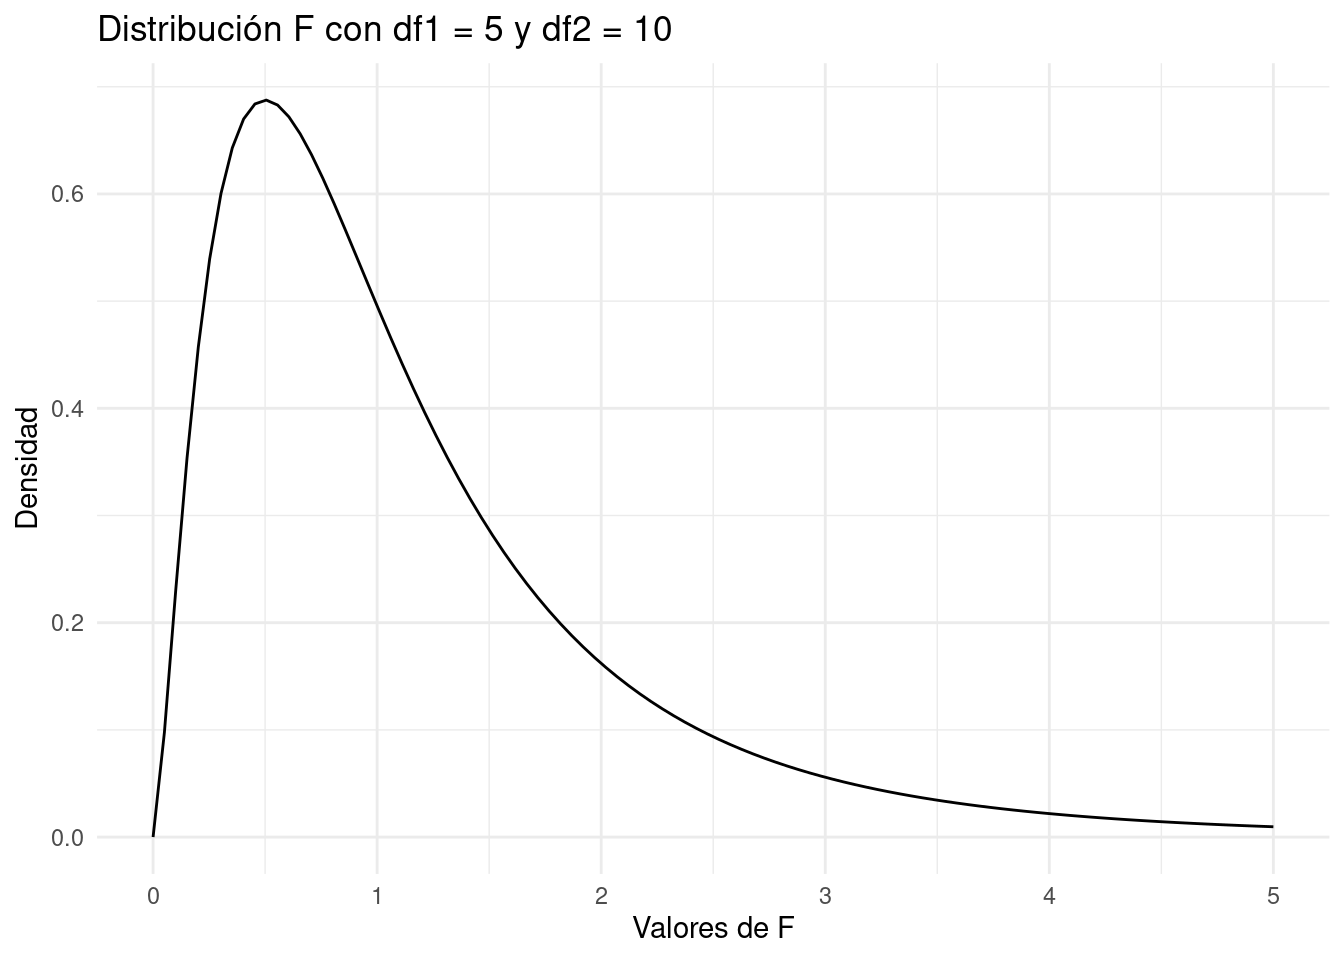
\includegraphics{anova_files/figure-pdf/Dist_f1-1.pdf}

}

\end{figure}

El gráfico muestra la densidad de la distribución F para los grados de
libertad especificados. La forma de la distribución F depende de los
valores de df1 y df2. Te animamos a que pruebes diferentes valores de
esos dos parámetros usando el código anterior.

Ahora, vamos a calcular valores específicos de la función de
distribución acumulativa (CDF) y la función de densidad (PDF) para un
valor de F.

\begin{Shaded}
\begin{Highlighting}[]
\CommentTok{\# Calcular el valor de la función de densidad (PDF) para F = 2}
\NormalTok{f\_value }\OtherTok{\textless{}{-}} \DecValTok{2}
\NormalTok{pdf\_value }\OtherTok{\textless{}{-}} \FunctionTok{df}\NormalTok{(f\_value, df1, df2)}
\FunctionTok{cat}\NormalTok{(}\StringTok{"PDF en F ="}\NormalTok{, f\_value, }\StringTok{"es"}\NormalTok{, pdf\_value, }\StringTok{"}\SpecialCharTok{\textbackslash{}n}\StringTok{"}\NormalTok{)}
\end{Highlighting}
\end{Shaded}

\begin{verbatim}
PDF en F = 2 es 0.1620057 
\end{verbatim}

\begin{Shaded}
\begin{Highlighting}[]
\CommentTok{\# Calcular el valor de la función de distribución acumulativa (CDF) para F = 2}
\NormalTok{cdf\_value }\OtherTok{\textless{}{-}} \FunctionTok{pf}\NormalTok{(f\_value, df1, df2)}
\FunctionTok{cat}\NormalTok{(}\StringTok{"CDF en F ="}\NormalTok{, f\_value, }\StringTok{"es"}\NormalTok{, cdf\_value, }\StringTok{"}\SpecialCharTok{\textbackslash{}n}\StringTok{"}\NormalTok{)}
\end{Highlighting}
\end{Shaded}

\begin{verbatim}
CDF en F = 2 es 0.835805 
\end{verbatim}

\begin{Shaded}
\begin{Highlighting}[]
\CommentTok{\# Calcular el valor crítico de F para un nivel de significancia del 5\%}
\NormalTok{alpha }\OtherTok{\textless{}{-}} \FloatTok{0.05}
\NormalTok{f\_critical }\OtherTok{\textless{}{-}} \FunctionTok{qf}\NormalTok{(}\DecValTok{1} \SpecialCharTok{{-}}\NormalTok{ alpha, df1, df2)}
\FunctionTok{cat}\NormalTok{(}\StringTok{"Valor crítico de F para un nivel de significancia del 5\% es"}\NormalTok{, f\_critical, }\StringTok{"}\SpecialCharTok{\textbackslash{}n}\StringTok{"}\NormalTok{)}
\end{Highlighting}
\end{Shaded}

\begin{verbatim}
Valor crítico de F para un nivel de significancia del 5% es 3.325835 
\end{verbatim}

El valor de la función de densidad para \(F = 2\) indica la densidad de
probabilidad en ese punto específico.

El valor de la CDF para \(F = 2\) indica la probabilidad acumulada de
obtener un valor de F menor o igual a \(2\).

El valor crítico de F para un nivel de significancia del \(\alpha=0.05\)
es el valor de F más allá del cual la probabilidad acumulada es \(5\%\).
Este valor se utiliza en pruebas estadísticas para decidir si se rechaza
o no la hipótesis nula.

\end{tcolorbox}

\hypertarget{modelo-con-un-factor}{%
\section{Modelo con un factor}\label{modelo-con-un-factor}}

El modelo de ANOVA de un factor se utiliza cuando se estudia el efecto
de un solo factor (variable independiente) en una variable dependiente
continua. Este modelo permite comparar las medias de varios grupos para
determinar si existen diferencias significativas entre ellos.

\begin{itemize}
\tightlist
\item
  \textbf{Hipótesis}:

  \begin{itemize}
  \tightlist
  \item
    \textbf{Hipótesis Nula (}\(H_0\)): Todas las medias de los grupos
    son iguales (\(\mu_1 = \mu_2 = \cdots = \mu_k\)).
  \item
    \textbf{Hipótesis Alternativa (}\(H_a\)): Al menos una de las medias
    de los grupos es diferente.
  \end{itemize}
\end{itemize}

Tenemos una variable aleatoria \(Y\) que toma valores reales y una
variable cualitativa o factor \(X\) con \(k\) niveles
\(1,2,\ldots,i,\ldots,k\). La variable \(Y\) toma valores
\(Y_{ij}, j=1,\ldots,n_i\) en el nivel \(i\) del factor \(X\), siendo
\(n_i\) el número de observaciones en el nivel \(i\) del factor \(X\).

Tenemos los siguientes supuestos:

\begin{itemize}
\tightlist
\item
  Normalidad: Las distribuciones de las poblaciones de las que provienen
  las muestras son normales.
\item
  Homogeneidad de varianzas: Las varianzas de las poblaciones son
  iguales.
\item
  Independencia: Las observaciones son independientes entre sí.
\end{itemize}

Escribimos el modelo como sigue: \[
  Y_{ij} = \mu + \tau_i + \epsilon_{ij}
\] Donde:

\begin{itemize}
\tightlist
\item
  \(Y_{ij}\) es la observación \(j\)-ésima del grupo \(i\)-ésimo.
\item
  \(\mu\) es la media general.
\item
  \(\epsilon_{ij}\) es el término de error aleatorio.
\item
  \(\tau_i\) es el efecto del grupo i-ésimo en la media de la variable
  respuesta \(Y\). Esto es, cuánto aumenta o disminuye la media de \(Y\)
  por pertenecer la observación a la categoría \(i\). De modo que
  podemos llamar \[
  Y_i=\mu+\tau_i
  \] al efecto medio del grupo \(i\)-esimo.
\end{itemize}

La Suma de las diferencias al cuadrado de cada dato respecto a la media
general se calcula como sigue: \[
    \text{SST} = \sum_{i=1}^{k} \sum_{j=1}^{n_i} (Y_{ij} - \bar{Y}_{..})^2        
\] donde \(\bar{Y}_{..}\) es la media general de todas las
observaciones.

Teniendo en cuenta que: \[
Y_{ij} - \bar{Y}_{..}= Y_i  + \epsilon_{ij} - \bar{Y}_{..} 
\] Podemos descomponer la suma de cuadrados, como sigue:

\[
    \text{SST} = \sum_{i=1}^{k} \sum_{j=1}^{n_i} (Y_{ij} - \bar{Y}_{..})^2=  \sum_{i=1}^{k} n_i (\bar{Y}_i - \bar{Y}_{..})^2+\sum_{i=1}^{k} \sum_{j=1}^{n_i} (Y_{ij} - \bar{Y}_i)^2      
\]

Donde: La varianza entre grupos se calcula como la suma de las
diferencias al cuadrado de las medias de los grupos respecto a la media
general, ponderada por el tamaño de los grupos: \[
\text{SSB} = \sum_{i=1}^{k} n_i (\bar{Y}_i - \bar{Y}_{..})^2
\] donde \(\bar{Y}_i\) es la media del grupo \(i\).

Además, la varianza dentro de los grupos, se calcula como la suma de las
diferencias al cuadrado de cada dato respecto a la media de su grupo se
obtiene como: \[
\text{SSW} = \sum_{i=1}^{k} \sum_{j=1}^{n_i} (Y_{ij} - \bar{Y}_i)^2
\] Esto es, se descompone la variabilidad total de los datos en dos
componentes, SSB que refleja la diferencia de cada grupo respecto a la
media global y SSW que refleja la variabilidad intrínseca dentro de cada
grupo: \[
\text{SST} = \text{SSB} + \text{SSW}
\]

\textbf{Cálculo del Estadístico F}: \[
F = \frac{\text{Varianza Entre Grupos (MSB)}}{\text{Varianza Dentro de los Grupos (MSW)}}
\] Donde:

\begin{itemize}
\tightlist
\item
  MSB (Mean Square Between): Media cuadrática entre grupos.
\item
  MSW (Mean Square Within): Media cuadrática dentro de los grupos.
\end{itemize}

Esto es: \[
F=\frac{SSB/df_B}{SSW/df_W}
\] donde:

\begin{itemize}
\tightlist
\item
  \(df_B=k-1\) son los grados de libertad entre los grupos
\item
  \(df_W=N-k\) son los grado sd elibertado dentro de los grupos, siendo
  \(N\) el número total de observaciones.
\end{itemize}

Una vez se dispone de toda esta información, es común representarla en
forma de tabla, en la llamada \emph{Tabla ANOVA}:

\begin{longtable}[]{@{}
  >{\raggedright\arraybackslash}p{(\columnwidth - 6\tabcolsep) * \real{0.3750}}
  >{\raggedright\arraybackslash}p{(\columnwidth - 6\tabcolsep) * \real{0.2083}}
  >{\raggedright\arraybackslash}p{(\columnwidth - 6\tabcolsep) * \real{0.2083}}
  >{\raggedright\arraybackslash}p{(\columnwidth - 6\tabcolsep) * \real{0.2083}}@{}}
\toprule\noalign{}
\begin{minipage}[b]{\linewidth}\raggedright
Fuente de variación
\end{minipage} & \begin{minipage}[b]{\linewidth}\raggedright
Suma de cuadrados
\end{minipage} & \begin{minipage}[b]{\linewidth}\raggedright
Grados de libertad
\end{minipage} & \begin{minipage}[b]{\linewidth}\raggedright
Cuadrado Medio
\end{minipage} \\
\midrule\noalign{}
\endhead
\bottomrule\noalign{}
\endlastfoot
Disferencias entre grupos & SSB & k-1 & MSB \\
Diferencias dentro de los grupos, Residual o Error & SSW & N-k & MSW \\
Total & SST & N-1 & \\
\end{longtable}

\begin{tcolorbox}[enhanced jigsaw, arc=.35mm, breakable, coltitle=black, left=2mm, opacityback=0, bottomtitle=1mm, colbacktitle=quarto-callout-caution-color!10!white, title=\textcolor{quarto-callout-caution-color}{\faFire}\hspace{0.5em}{Para el futuro}, titlerule=0mm, colback=white, colframe=quarto-callout-caution-color-frame, bottomrule=.15mm, rightrule=.15mm, opacitybacktitle=0.6, toptitle=1mm, toprule=.15mm, leftrule=.75mm]

La proporción de variabilidad explicada por los grupos se calcula como:
\[
R^2=1-SSW/SST
\] Este valor, será muy importante en la asignatura de \emph{Regresión}
del Grado en Ciencia e Ingeniería de Datos.

\end{tcolorbox}

El estadístico de prueba \(F \sim F_{df_B,df_W}\) bajo la hipótesis nula
de igualdad de medias.

El \(p-valor\) se obtiene a partir de la distribución \(F\),
considerando los grados de libertad de los numeradores y denominadores.
Esto es: \[
p-valor=P(F_{df_b,df_W}>F_{muestral})
\]

Como en otros contrastes, si el \(p-valor\) p es menor que el nivel de
significancia (\(\alpha\)), se rechaza la hipótesis nula, concluyendo
que al menos una de las medias de los grupos es diferente.

\begin{tcolorbox}[enhanced jigsaw, arc=.35mm, breakable, coltitle=black, left=2mm, opacityback=0, bottomtitle=1mm, colbacktitle=quarto-callout-tip-color!10!white, title=\textcolor{quarto-callout-tip-color}{\faLightbulb}\hspace{0.5em}{Ejemplo. ANOVA de un factor}, titlerule=0mm, colback=white, colframe=quarto-callout-tip-color-frame, bottomrule=.15mm, rightrule=.15mm, opacitybacktitle=0.6, toptitle=1mm, toprule=.15mm, leftrule=.75mm]

Vamos a realizar un ejemplo completo de ANOVA de un factor, donde
calcularemos todos los pasos del contraste, incluidos el valor de F y el
p-valor.

Supongamos que tenemos tres tratamientos (A, B y C) y sus
correspondientes muestras de datos son:

\begin{itemize}
\tightlist
\item
  Grupo A: \([5, 7, 6, 9, 6]\)
\item
  Grupo B: \([8, 12, 9, 11, 10]\)
\item
  Grupo C: \([14, 10, 13, 15, 12]\)
\end{itemize}

Nuestro objetivo es determinar si existe una diferencia significativa
entre las medias de estos tres grupos.

En primer lugar calculamos la media de cada grupo y la media general:

\begin{itemize}
\item
  Media de Grupo A (\(\bar{Y}_A\)): \[
  \bar{Y}_A = \frac{5 + 7 + 6 + 9 + 6}{5} = \frac{33}{5} = 6.6
  \]
\item
  Media de Grupo B (\(\bar{Y}_B\)): \[
  \bar{Y}_B = \frac{8 + 12 + 9 + 11 + 10}{5} = \frac{50}{5} = 10.0
  \]
\item
  Media de Grupo C (\(\bar{Y}_C\)): \[
  \bar{Y}_C = \frac{14 + 10 + 13 + 15 + 12}{5} = \frac{64}{5} = 12.8
  \]
\item
  Media General (\(\bar{Y}\)): \[
  \bar{Y} = \frac{6.6 + 10.0 + 12.8}{3} = \frac{29.4}{3} \approx 9.8
  \]
\end{itemize}

Calculamos la Suma de Cuadrados entre Grupos (SSB)

\[
\text{SSB} = n_A (\bar{Y}_A - \bar{Y})^2 + n_B (\bar{Y}_B - \bar{Y})^2 + n_C (\bar{Y}_C - \bar{Y})^2
\] donde \(n_A = n_B = n_C = 5\) (número de observaciones en cada
grupo). Fíjate que el número de observaciones en cada grupo podría ser
diferente. En este ejemplo, son iguales.

\[
\text{SSB} = 5 (6.6 - 9.8)^2 + 5 (10.0 - 9.8)^2 + 5 (12.8 - 9.8)^2 =96.4
\]

A continuación calculamos la Suma de Cuadrados Dentro de los Grupos
(SSW)

\[
\text{SSW} = \sum_{i=1}^{k} \sum_{j=1}^{n_i} (Y_{ij} - \bar{Y}_i)^2
\]

Para cada grupo, calculamos la suma de las diferencias al cuadrado entre
cada dato y la media del grupo:

\begin{itemize}
\item
  Grupo A: \[
  (5 - 6.6)^2 + (7 - 6.6)^2 + (6 - 6.6)^2 + (9 - 6.6)^2 + (6 - 6.6)^2 = 9.2
  \]
\item
  Grupo B: \[
  (8 - 10.0)^2 + (12 - 10.0)^2 + (9 - 10.0)^2 + (11 - 10.0)^2 + (10 - 10.0)^2 = 10.0
  \]
\item
  Grupo C: \[
  (14 - 12.8)^2 + (10 - 12.8)^2 + (13 - 12.8)^2 + (15 - 12.8)^2 + (12 - 12.8)^2 = 14.8
  \]
\end{itemize}

Entonces, la Suma de Cuadrados Dentro de los Grupos (SSW) es: \[
\text{SSW} = 9.2 + 10.0 + 14.8 = 34.0
\]

Tenemos, por tanto que la Suma Total de Cuadrados (SST) es: \[
\text{SST} = \text{SSB} + \text{SSW} = 96.4 + 34.0 = 130.4
\]

Para realizar el contraste, necesitamos calcular los Grados de Libertad
del estadístico:

\begin{itemize}
\tightlist
\item
  Grados de libertad entre los grupos (\(\text{df}_B = k-1=3-1=2\)):
\item
  Grados de libertad dentro de los grupos (\(\text{df}_W=N-k=15-3=12\)):
\end{itemize}

Calcularemos las varianzas como sigue:

\begin{itemize}
\item
  Varianza entre los grupos (MSB): \[
  \text{MSB} = \frac{\text{SSB}}{\text{df}_B} = \frac{96.4}{2} = 48.2
  \]
\item
  Varianza dentro de los grupos (MSW): \[
  \text{MSW} = \frac{\text{SSW}}{\text{df}_W} = \frac{34.0}{12} \approx 2.8333
  \]
\end{itemize}

Ya estamos en disposición de calcular el estadístico de contraste : \[
F = \frac{\text{MSB}}{\text{MSW}} = \frac{48.2}{2.8333} \approx 17.01
\]

El p-valor se obtiene utilizando la distribución \(F\) con
\(\text{df}_B = 2\) y \(\text{df}_W = 12\). Para este ejemplo, podemos
utilizar software estadístico o tablas de distribución F.

Usando R:

\begin{Shaded}
\begin{Highlighting}[]
\FunctionTok{pf}\NormalTok{(}\FloatTok{17.01}\NormalTok{, }\AttributeTok{df1 =} \DecValTok{2}\NormalTok{, }\AttributeTok{df2 =} \DecValTok{12}\NormalTok{, }\AttributeTok{lower.tail =} \ConstantTok{FALSE}\NormalTok{)}
\end{Highlighting}
\end{Shaded}

\begin{verbatim}
[1] 0.0003143459
\end{verbatim}

El p-valor es muy pequeño, mucho menor que el grado de significancia
\(\alpha=0.05\), indicando una diferencia significativa entre los
grupos.

\end{tcolorbox}

\hypertarget{modelo-con-dos-factores-con-y-sin-interacciuxf3n}{%
\section{Modelo con dos factores con y sin
Interacción}\label{modelo-con-dos-factores-con-y-sin-interacciuxf3n}}

El modelo de ANOVA de dos factores se utiliza cuando se estudian dos
factores simultáneamente para evaluar su efecto individual y conjunto en
una variable dependiente. Podemos verlo como una generalización del caso
de ANOVA con un único factor. Este modelo es más complejo y permite
entender no solo los efectos principales de cada factor, sino también si
hay una interacción entre ellos.

Sean A y B dos factores que se desean estudiar, con \(m_A\) y \(m_B\)
niveles. Trabajaremos con las siguientes hipótesis nulas:

\begin{itemize}
\tightlist
\item
  \textbf{Hipótesis}:

  \begin{itemize}
  \tightlist
  \item
    \textbf{Hipótesis Nula para los efectos principales (}\(H_0\)):

    \begin{itemize}
    \tightlist
    \item
      No hay efecto del primer factor.
    \item
      No hay efecto del segundo factor.
    \end{itemize}
  \item
    \textbf{Hipótesis Nula para la interacción (}\(H_0\)): No hay
    interacción entre los dos factores.
  \end{itemize}
\end{itemize}

\textbf{Modelo sin Interacción}:

\[ Y_{ijk} = \mu + \alpha_i + \beta_j + \epsilon_{ijk} \]

Donde:

\begin{itemize}
\tightlist
\item
  \(Y_{ijk}\) es la observación \(k\)-ésima del nivel \(j\)-ésimo del
  factor B y nivel \(i\)-ésimo del factor A. - \(\mu\) es la media
  general.
\item
  \(\alpha_i\) es el efecto del nivel \(i\)-ésimo del factor A.
\item
  \(\beta_j\) es el efecto del nivel \(j\)-ésimo del factor B. -
  \(\epsilon_{ijk}\) es el término de error aleatorio.
\end{itemize}

En este caso, la tabla ANOVA queda como sigue:

\begin{longtable}[]{@{}
  >{\raggedright\arraybackslash}p{(\columnwidth - 6\tabcolsep) * \real{0.3750}}
  >{\raggedright\arraybackslash}p{(\columnwidth - 6\tabcolsep) * \real{0.2083}}
  >{\raggedright\arraybackslash}p{(\columnwidth - 6\tabcolsep) * \real{0.2083}}
  >{\raggedright\arraybackslash}p{(\columnwidth - 6\tabcolsep) * \real{0.2083}}@{}}
\toprule\noalign{}
\begin{minipage}[b]{\linewidth}\raggedright
Fuente de variación
\end{minipage} & \begin{minipage}[b]{\linewidth}\raggedright
Suma de cuadrados
\end{minipage} & \begin{minipage}[b]{\linewidth}\raggedright
Grados de libertad
\end{minipage} & \begin{minipage}[b]{\linewidth}\raggedright
Cuadrado Medio
\end{minipage} \\
\midrule\noalign{}
\endhead
\bottomrule\noalign{}
\endlastfoot
Diferencias entre niveles del factor A & \(SSB_A\) & \(m_A-1\) &
\(MSB_A\) \\
Diferencias entre niveles del factor B & \(SSB_B\) & \(m_B-1\) &
\(MSB_B\) \\
Error & \(SSW\) & \(N-m_A-m_B+1\) & \(MSW\) \\
Total & \(SST\) & \(N-1\) & \\
\end{longtable}

Para estudiar la importancia de cada factor se calcula el estadístico
\(F\) particular para cada uno de ellos como sigue: \[
F_A=\frac{MSB_A}{MSW} \sim F_{m_A-1,N-m_A-m_B+1}
\] y \[
F_B=\frac{MSB_B}{MSW}\sim F_{m_B-1,N-m_A-m_B+1}
\] A partir de estos estadísticos de prueba podemos contrastar las
hipótesis nulas de no existencia de efectos asociados a los factores
\(A\) y \(B\) respectivamente.

\textbf{Modelo con Interacción}:
\[ Y_{ijk} = \mu + \alpha_i + \beta_j + (\alpha\beta)_{ij} + \epsilon_{ijk} \]

Donde: \((\alpha\beta)_{ij}\) representa el efecto de interacción entre
el nivel \(i\)-ésimo del factor A y el nivel \(j\)-ésimo del factor B.

En este caso, la tabla ANOVA añade el factor de interacción:

\begin{longtable}[]{@{}
  >{\raggedright\arraybackslash}p{(\columnwidth - 6\tabcolsep) * \real{0.3750}}
  >{\raggedright\arraybackslash}p{(\columnwidth - 6\tabcolsep) * \real{0.2083}}
  >{\raggedright\arraybackslash}p{(\columnwidth - 6\tabcolsep) * \real{0.2083}}
  >{\raggedright\arraybackslash}p{(\columnwidth - 6\tabcolsep) * \real{0.2083}}@{}}
\toprule\noalign{}
\begin{minipage}[b]{\linewidth}\raggedright
Fuente de variación
\end{minipage} & \begin{minipage}[b]{\linewidth}\raggedright
Suma de cuadrados
\end{minipage} & \begin{minipage}[b]{\linewidth}\raggedright
Grados de libertad
\end{minipage} & \begin{minipage}[b]{\linewidth}\raggedright
Cuadrado Medio
\end{minipage} \\
\midrule\noalign{}
\endhead
\bottomrule\noalign{}
\endlastfoot
Diferencias entre niveles del factor A & \(SSB_A\) & \(m_A-1\) &
\(MSB_A\) \\
Diferencias entre niveles del factor B & \(SSB_B\) & \(m_B-1\) &
\(MSB_B\) \\
Diferencias debidas la interacción & \(SSB_{AB}\) & \((m_A-1)*(m_B-1)\)
& \(MSB_{AB}\) \\
Error & \(SSW\) & \(N-m_A*m_B\) & \(MSW\) \\
Total & \(SST\) & \(N-1\) & \\
\end{longtable}

Para estudiar la importancia de cada de la interacción se calculan el
estadístico \(F\) correspondiente:

\[
F_{AB}=\frac{MSB_{AB}}{MSW}\sim F_{(m_A-1)*(m_B-1),N-m_A*m_B}
\]

A partir de este estadísticos de prueba podemos contrastar la hipótesis
nula de no existencia de interacción entre los dos factores \(A\),
\(B\). Si podemos rechazar esa hipótesis, es decir, si existe
interacción entre los factores, entonces hemos terminado. Es decir, no
podemos eliminar ningún factor del modelo. En cambio, si no rechazamos
la hipótesis nula, es decir, si no existe interacción entre los
factores, podemos eliminar dicho efecto (la interacción) del modelo y
pasar a un modelos sin interacción como el anteriormente descrito.

\begin{tcolorbox}[enhanced jigsaw, arc=.35mm, breakable, coltitle=black, left=2mm, opacityback=0, bottomtitle=1mm, colbacktitle=quarto-callout-tip-color!10!white, title=\textcolor{quarto-callout-tip-color}{\faLightbulb}\hspace{0.5em}{Ejemplo. ANOVA de dos factores con interacción}, titlerule=0mm, colback=white, colframe=quarto-callout-tip-color-frame, bottomrule=.15mm, rightrule=.15mm, opacitybacktitle=0.6, toptitle=1mm, toprule=.15mm, leftrule=.75mm]

Supongamos que estamos estudiando el efecto de dos factores sobre el
rendimiento de los estudiantes: el método de enseñanza (con dos niveles:
Tradicional y Experimental) y el tipo de material de estudio (con tres
niveles: Libro, Video, y Online). Queremos saber si estos factores, y su
posible interacción, tienen un efecto significativo en el rendimiento.

\begin{Shaded}
\begin{Highlighting}[]
\NormalTok{rendimiento }\OtherTok{\textless{}{-}} \FunctionTok{c}\NormalTok{(}\DecValTok{85}\NormalTok{, }\DecValTok{88}\NormalTok{, }\DecValTok{90}\NormalTok{, }\DecValTok{83}\NormalTok{, }\DecValTok{87}\NormalTok{, }\DecValTok{85}\NormalTok{, }\DecValTok{86}\NormalTok{, }\DecValTok{89}\NormalTok{, }\DecValTok{91}\NormalTok{, }\DecValTok{84}\NormalTok{, }\DecValTok{88}\NormalTok{, }\DecValTok{87}\NormalTok{,}
                 \DecValTok{78}\NormalTok{, }\DecValTok{79}\NormalTok{, }\DecValTok{80}\NormalTok{, }\DecValTok{76}\NormalTok{, }\DecValTok{77}\NormalTok{, }\DecValTok{75}\NormalTok{, }\DecValTok{78}\NormalTok{, }\DecValTok{79}\NormalTok{, }\DecValTok{81}\NormalTok{, }\DecValTok{76}\NormalTok{, }\DecValTok{77}\NormalTok{, }\DecValTok{76}\NormalTok{,}
                 \DecValTok{90}\NormalTok{, }\DecValTok{92}\NormalTok{, }\DecValTok{91}\NormalTok{, }\DecValTok{93}\NormalTok{, }\DecValTok{90}\NormalTok{, }\DecValTok{89}\NormalTok{, }\DecValTok{91}\NormalTok{, }\DecValTok{92}\NormalTok{, }\DecValTok{91}\NormalTok{, }\DecValTok{93}\NormalTok{, }\DecValTok{92}\NormalTok{, }\DecValTok{91}\NormalTok{)}
\NormalTok{metodo }\OtherTok{\textless{}{-}} \FunctionTok{factor}\NormalTok{(}\FunctionTok{rep}\NormalTok{(}\FunctionTok{c}\NormalTok{(}\StringTok{"Tradicional"}\NormalTok{, }\StringTok{"Experimental"}\NormalTok{), }\AttributeTok{each=}\DecValTok{18}\NormalTok{))}
\NormalTok{material }\OtherTok{\textless{}{-}} \FunctionTok{factor}\NormalTok{(}\FunctionTok{rep}\NormalTok{(}\FunctionTok{c}\NormalTok{(}\StringTok{"Libro"}\NormalTok{, }\StringTok{"Video"}\NormalTok{, }\StringTok{"Online"}\NormalTok{), }\AttributeTok{each=}\DecValTok{6}\NormalTok{, }\AttributeTok{times=}\DecValTok{2}\NormalTok{))}

\CommentTok{\# Crear un data frame}
\NormalTok{datos }\OtherTok{\textless{}{-}} \FunctionTok{data.frame}\NormalTok{(rendimiento, metodo, material)}

\CommentTok{\# Visualizar los datos}
\FunctionTok{library}\NormalTok{(}\StringTok{"ggpubr"}\NormalTok{)}
\FunctionTok{ggline}\NormalTok{(datos, }\AttributeTok{x =} \StringTok{"material"}\NormalTok{, }\AttributeTok{y =} \StringTok{"rendimiento"}\NormalTok{, }\AttributeTok{color =} \StringTok{"metodo"}\NormalTok{,}
       \AttributeTok{add =} \FunctionTok{c}\NormalTok{(}\StringTok{"mean\_se"}\NormalTok{, }\StringTok{"dotplot"}\NormalTok{),}
       \AttributeTok{palette =} \FunctionTok{c}\NormalTok{(}\StringTok{"\#00AFBB"}\NormalTok{, }\StringTok{"\#E7B800"}\NormalTok{))}
\end{Highlighting}
\end{Shaded}

\begin{verbatim}
Bin width defaults to 1/30 of the range of the data. Pick better value with
`binwidth`.
\end{verbatim}

\begin{figure}[H]

{\centering 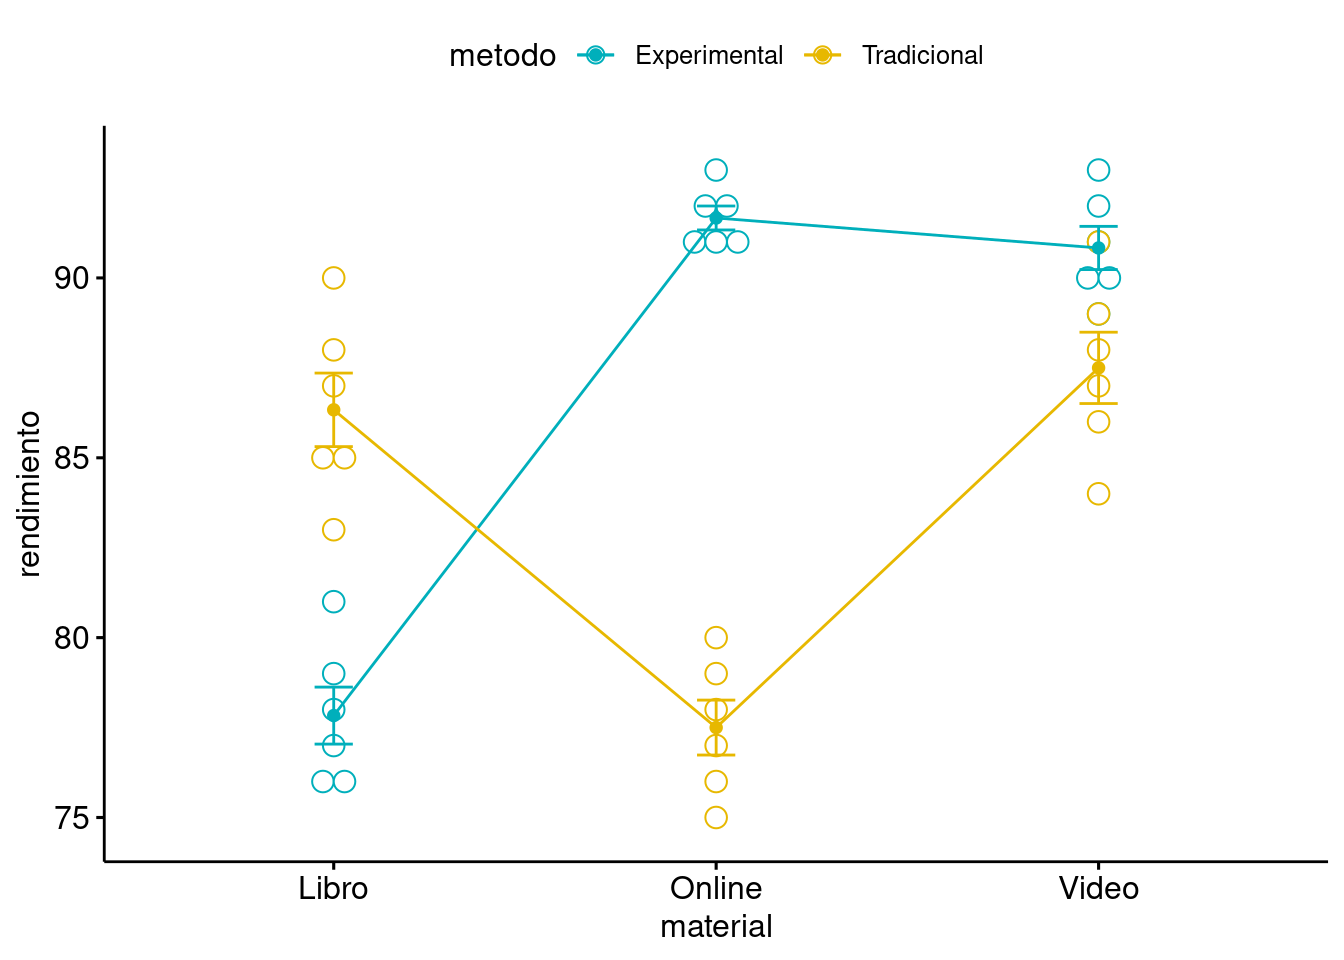
\includegraphics{anova_files/figure-pdf/datos_anova-1.pdf}

}

\end{figure}

Ahora que tenemos nuestros datos, vamos a realizar el ANOVA de dos
factores con interacción.

\begin{Shaded}
\begin{Highlighting}[]
\CommentTok{\# Realizar el ANOVA de dos factores con interacción}
\NormalTok{anova\_result }\OtherTok{\textless{}{-}} \FunctionTok{aov}\NormalTok{(rendimiento }\SpecialCharTok{\textasciitilde{}}\NormalTok{ metodo }\SpecialCharTok{*}\NormalTok{ material, }\AttributeTok{data=}\NormalTok{datos)}

\CommentTok{\# Mostrar los resultados del ANOVA}
\FunctionTok{summary}\NormalTok{(anova\_result)}
\end{Highlighting}
\end{Shaded}

\begin{verbatim}
                Df Sum Sq Mean Sq F value   Pr(>F)    
metodo           1   81.0    81.0   21.83 5.88e-05 ***
material         2  309.7   154.9   41.73 2.16e-09 ***
metodo:material  2  771.2   385.6  103.90 3.26e-14 ***
Residuals       30  111.3     3.7                     
---
Signif. codes:  0 '***' 0.001 '**' 0.01 '*' 0.05 '.' 0.1 ' ' 1
\end{verbatim}

Los resultados del ANOVA se interpretan observando los \(p-valores\)
para cada uno de los componentes del modelo:

\begin{itemize}
\tightlist
\item
  \textbf{metodo}: Efecto principal del método de enseñanza.
\item
  \textbf{material}: Efecto principal del tipo de material de estudio.
\item
  \textbf{metodo:material}: Interacción entre el método de enseñanza y
  el tipo de material de estudio.
\end{itemize}

El \(p-valor\) asociado a la interacción es menor que \(0.05\), lo que
indica que la interacción entre el método de enseñanza y el tipo de
material de estudio es significativa y por lo tanto no debe ser
eliminada del modelo.

Efectivamente, viendo la figura anterior concluimos que el rendimiento
depende de la interacción entre los dos factores. Así, por ejemplo,
cuando el matería es proporcionado de modo ``online'' o en ``vídeo'' el
rendimiento es más elevado en el método experimental que en el método
tradicional. La diferencia entre los dos métodos es especialmente
notable cuando el material es ``online''. Sin embargo, cuando el
material se ofrece en modo ``libro'' el método tradicional ofrece
mejores resultados que el método experimental.

\end{tcolorbox}

\begin{tcolorbox}[enhanced jigsaw, arc=.35mm, breakable, coltitle=black, left=2mm, opacityback=0, bottomtitle=1mm, colbacktitle=quarto-callout-tip-color!10!white, title=\textcolor{quarto-callout-tip-color}{\faLightbulb}\hspace{0.5em}{Ejemplo. ANOVA de dos factores no significativos}, titlerule=0mm, colback=white, colframe=quarto-callout-tip-color-frame, bottomrule=.15mm, rightrule=.15mm, opacitybacktitle=0.6, toptitle=1mm, toprule=.15mm, leftrule=.75mm]

Supongamos que estamos estudiando el efecto del tipo de fertilizante
(con dos niveles: \(A\) y \(B\)) y el tipo de riego (con tres niveles:
Goteo, Aspersión, Manual) sobre el crecimiento de las plantas.

En primer lugar observamos los datos:

\begin{Shaded}
\begin{Highlighting}[]
\CommentTok{\# Crear datos simulados}
\NormalTok{crecimiento }\OtherTok{\textless{}{-}} \FunctionTok{c}\NormalTok{(}\DecValTok{20}\NormalTok{, }\DecValTok{21}\NormalTok{, }\DecValTok{23}\NormalTok{, }\DecValTok{22}\NormalTok{, }\DecValTok{24}\NormalTok{, }\DecValTok{25}\NormalTok{, }\DecValTok{26}\NormalTok{, }\DecValTok{27}\NormalTok{, }\DecValTok{28}\NormalTok{, }\DecValTok{29}\NormalTok{, }\DecValTok{30}\NormalTok{, }\DecValTok{31}\NormalTok{,}
                 \DecValTok{22}\NormalTok{, }\DecValTok{23}\NormalTok{, }\DecValTok{25}\NormalTok{, }\DecValTok{24}\NormalTok{, }\DecValTok{26}\NormalTok{, }\DecValTok{27}\NormalTok{, }\DecValTok{28}\NormalTok{, }\DecValTok{29}\NormalTok{, }\DecValTok{30}\NormalTok{, }\DecValTok{31}\NormalTok{, }\DecValTok{32}\NormalTok{, }\DecValTok{33}\NormalTok{,}
                 \DecValTok{21}\NormalTok{, }\DecValTok{23}\NormalTok{, }\DecValTok{22}\NormalTok{, }\DecValTok{24}\NormalTok{, }\DecValTok{23}\NormalTok{, }\DecValTok{25}\NormalTok{, }\DecValTok{26}\NormalTok{, }\DecValTok{28}\NormalTok{, }\DecValTok{27}\NormalTok{, }\DecValTok{29}\NormalTok{, }\DecValTok{28}\NormalTok{, }\DecValTok{30}\NormalTok{)}
\NormalTok{fertilizante }\OtherTok{\textless{}{-}} \FunctionTok{factor}\NormalTok{(}\FunctionTok{rep}\NormalTok{(}\FunctionTok{c}\NormalTok{(}\StringTok{"A"}\NormalTok{, }\StringTok{"B"}\NormalTok{), }\AttributeTok{each=}\DecValTok{18}\NormalTok{))}
\NormalTok{riego }\OtherTok{\textless{}{-}} \FunctionTok{factor}\NormalTok{(}\FunctionTok{rep}\NormalTok{(}\FunctionTok{c}\NormalTok{(}\StringTok{"Goteo"}\NormalTok{, }\StringTok{"Aspersión"}\NormalTok{, }\StringTok{"Manual"}\NormalTok{), }\AttributeTok{each=}\DecValTok{6}\NormalTok{, }\AttributeTok{times=}\DecValTok{2}\NormalTok{))}

\CommentTok{\# Crear un data frame}
\NormalTok{datos }\OtherTok{\textless{}{-}} \FunctionTok{data.frame}\NormalTok{(crecimiento, fertilizante, riego)}

\CommentTok{\# Visualizar los datos}
\FunctionTok{library}\NormalTok{(}\StringTok{"ggpubr"}\NormalTok{)}
\FunctionTok{ggline}\NormalTok{(datos, }\AttributeTok{x =} \StringTok{"riego"}\NormalTok{, }\AttributeTok{y =} \StringTok{"crecimiento"}\NormalTok{, }\AttributeTok{color =} \StringTok{"fertilizante"}\NormalTok{,}
       \AttributeTok{add =} \FunctionTok{c}\NormalTok{(}\StringTok{"mean\_se"}\NormalTok{, }\StringTok{"dotplot"}\NormalTok{),}
       \AttributeTok{palette =} \FunctionTok{c}\NormalTok{(}\StringTok{"\#00AFBB"}\NormalTok{, }\StringTok{"\#E7B800"}\NormalTok{))}
\end{Highlighting}
\end{Shaded}

\begin{verbatim}
Bin width defaults to 1/30 of the range of the data. Pick better value with
`binwidth`.
\end{verbatim}

\begin{figure}[H]

{\centering 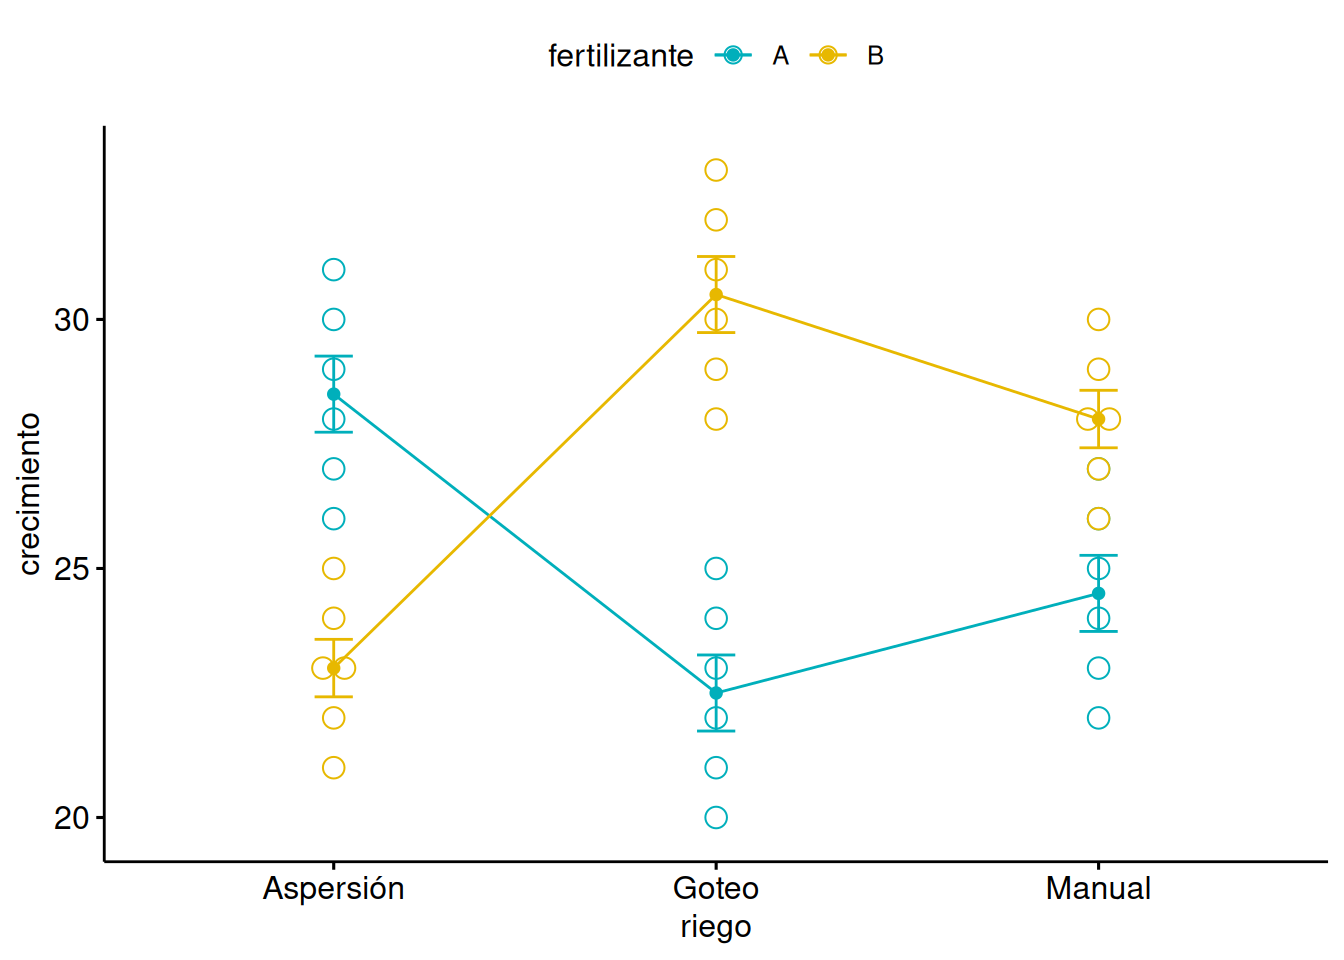
\includegraphics{anova_files/figure-pdf/datos_anova2-1.pdf}

}

\end{figure}

Realizamos el ANOVA de dos factores con interacción.

\begin{Shaded}
\begin{Highlighting}[]
\CommentTok{\# Realizar el ANOVA de dos factores con interacción}
\NormalTok{anova\_result }\OtherTok{\textless{}{-}} \FunctionTok{aov}\NormalTok{(crecimiento }\SpecialCharTok{\textasciitilde{}}\NormalTok{ fertilizante }\SpecialCharTok{*}\NormalTok{ riego, }\AttributeTok{data=}\NormalTok{datos)}

\CommentTok{\# Mostrar los resultados del ANOVA}
\FunctionTok{summary}\NormalTok{(anova\_result)}
\end{Highlighting}
\end{Shaded}

\begin{verbatim}
                   Df Sum Sq Mean Sq F value   Pr(>F)    
fertilizante        1   36.0   36.00  12.000  0.00162 ** 
riego               2    3.5    1.75   0.583  0.56424    
fertilizante:riego  2  283.5  141.75  47.250 5.36e-10 ***
Residuals          30   90.0    3.00                     
---
Signif. codes:  0 '***' 0.001 '**' 0.01 '*' 0.05 '.' 0.1 ' ' 1
\end{verbatim}

El \(p-valor\) asociado a la interaccióni es mayor que \(0.05\) lo, lo
que indica que la interacción entre el tipo de fertilizante y el tipo de
riego no es significativa y debe de ser eliminada del modelo.

Por tanto, obtenemos la tabla ANOVA para los dos factores sin
interacción:

\begin{Shaded}
\begin{Highlighting}[]
\CommentTok{\# Realizar el ANOVA de dos factores sin interacción}
\NormalTok{anova\_result }\OtherTok{\textless{}{-}} \FunctionTok{aov}\NormalTok{(crecimiento }\SpecialCharTok{\textasciitilde{}}\NormalTok{ fertilizante }\SpecialCharTok{+}\NormalTok{ riego, }\AttributeTok{data=}\NormalTok{datos)}

\CommentTok{\# Mostrar los resultados del ANOVA}
\FunctionTok{summary}\NormalTok{(anova\_result)}
\end{Highlighting}
\end{Shaded}

\begin{verbatim}
             Df Sum Sq Mean Sq F value Pr(>F)  
fertilizante  1   36.0   36.00   3.084 0.0886 .
riego         2    3.5    1.75   0.150 0.8614  
Residuals    32  373.5   11.67                 
---
Signif. codes:  0 '***' 0.001 '**' 0.01 '*' 0.05 '.' 0.1 ' ' 1
\end{verbatim}

Una vez eliminado el efecto de la interacción del modelo, podemos
observar como ninguno de los dos factores para estadísticamente
significativo, puesto que los \(p-valores\) asociados son mayores que
\(0.05\). Sin embargo, hemos de actuar con cautela. Veamos el modelo
cuando se elimina el factor menos significativo \texttt{riego}:

\begin{Shaded}
\begin{Highlighting}[]
\CommentTok{\# Realizar el ANOVA de un factor}
\NormalTok{anova\_result }\OtherTok{\textless{}{-}} \FunctionTok{aov}\NormalTok{(crecimiento }\SpecialCharTok{\textasciitilde{}}\NormalTok{ fertilizante, }\AttributeTok{data=}\NormalTok{datos)}

\CommentTok{\# Mostrar los resultados del ANOVA}
\FunctionTok{summary}\NormalTok{(anova\_result)}
\end{Highlighting}
\end{Shaded}

\begin{verbatim}
             Df Sum Sq Mean Sq F value Pr(>F)  
fertilizante  1     36   36.00   3.247 0.0804 .
Residuals    34    377   11.09                 
---
Signif. codes:  0 '***' 0.001 '**' 0.01 '*' 0.05 '.' 0.1 ' ' 1
\end{verbatim}

Al nivel de significancia estadística de \(0.05\) podríamos decir que el
factor \texttt{fertilizante} no es estadísticamente significativo y que
ninguno de los dos factores influye en el crecimiento de las planteas.

Ahora bien, si tuvieras que elegir un método de riego y un fertilizando,
¿cuál recomendarías al cliente? ¿por qué?

\end{tcolorbox}

\begin{tcolorbox}[enhanced jigsaw, arc=.35mm, breakable, coltitle=black, left=2mm, opacityback=0, bottomtitle=1mm, colbacktitle=quarto-callout-tip-color!10!white, title=\textcolor{quarto-callout-tip-color}{\faLightbulb}\hspace{0.5em}{Ejemplo. ANOVA de dos factores sin interacción}, titlerule=0mm, colback=white, colframe=quarto-callout-tip-color-frame, bottomrule=.15mm, rightrule=.15mm, opacitybacktitle=0.6, toptitle=1mm, toprule=.15mm, leftrule=.75mm]

Supongamos que estamos estudiando del tiempo de estudio y del tipo de
dieta en el rendimiento académico de un grupo de estudiantes. El tiempo
de estudio tiene \(3\) niveles (Alto, Medio y Bajo). El tipo de dieta
tiene \(3\) niveles (Normal, Vegana y Vegetariana).

En primer lugar observamos los datos:

\begin{Shaded}
\begin{Highlighting}[]
\CommentTok{\# Datos}
\NormalTok{datos }\OtherTok{\textless{}{-}} \FunctionTok{data.frame}\NormalTok{(}
  \AttributeTok{Tiempo\_estudio =} \FunctionTok{factor}\NormalTok{(}\FunctionTok{rep}\NormalTok{(}\FunctionTok{c}\NormalTok{(}\StringTok{"1. Alto"}\NormalTok{, }\StringTok{"2. Medio"}\NormalTok{, }\StringTok{"3. Bajo"}\NormalTok{), }\AttributeTok{each =} \DecValTok{9}\NormalTok{)),}
  \AttributeTok{Tipo\_dieta =} \FunctionTok{factor}\NormalTok{(}\FunctionTok{rep}\NormalTok{(}\FunctionTok{c}\NormalTok{(}\StringTok{"Vegetariana"}\NormalTok{, }\StringTok{"Normal"}\NormalTok{, }\StringTok{"Vegana"}\NormalTok{), }\AttributeTok{times =} \DecValTok{9}\NormalTok{)),}
  \AttributeTok{Rendimiento =} \FunctionTok{c}\NormalTok{(}\DecValTok{81}\NormalTok{, }\DecValTok{71}\NormalTok{, }\DecValTok{90}\NormalTok{, }\DecValTok{75}\NormalTok{, }\DecValTok{84}\NormalTok{, }\DecValTok{81}\NormalTok{, }\DecValTok{91}\NormalTok{, }\DecValTok{100}\NormalTok{, }\DecValTok{98}\NormalTok{, }\CommentTok{\# Datos para Nivel1 de Factor1}
                \DecValTok{60}\NormalTok{, }\DecValTok{83}\NormalTok{, }\DecValTok{70}\NormalTok{, }\DecValTok{54}\NormalTok{, }\DecValTok{65}\NormalTok{, }\DecValTok{73}\NormalTok{, }\DecValTok{82}\NormalTok{, }\DecValTok{92}\NormalTok{, }\DecValTok{73}\NormalTok{, }\CommentTok{\# Datos para Nivel2 de Factor1}
                \DecValTok{47}\NormalTok{, }\DecValTok{63}\NormalTok{, }\DecValTok{44}\NormalTok{, }\DecValTok{61}\NormalTok{, }\DecValTok{55}\NormalTok{, }\DecValTok{52}\NormalTok{, }\DecValTok{73}\NormalTok{, }\DecValTok{63}\NormalTok{, }\DecValTok{53}\NormalTok{) }\CommentTok{\# Datos para Nivel3 de Factor1}
\NormalTok{)}

\CommentTok{\# Visualizar}
\FunctionTok{library}\NormalTok{(}\StringTok{"ggpubr"}\NormalTok{)}
\FunctionTok{ggline}\NormalTok{(datos, }\AttributeTok{x =} \StringTok{"Tiempo\_estudio"}\NormalTok{, }\AttributeTok{y =} \StringTok{"Rendimiento"}\NormalTok{, }\AttributeTok{color =} \StringTok{"Tipo\_dieta"}\NormalTok{,}
       \AttributeTok{add =} \FunctionTok{c}\NormalTok{(}\StringTok{"mean\_se"}\NormalTok{, }\StringTok{"dotplot"}\NormalTok{),}
       \AttributeTok{palette =} \FunctionTok{c}\NormalTok{(}\StringTok{"\#00AFBB"}\NormalTok{, }\StringTok{"\#E7B800"}\NormalTok{,}\StringTok{"\#c94545"}\NormalTok{))}
\end{Highlighting}
\end{Shaded}

\begin{verbatim}
Bin width defaults to 1/30 of the range of the data. Pick better value with
`binwidth`.
\end{verbatim}

\begin{figure}[H]

{\centering 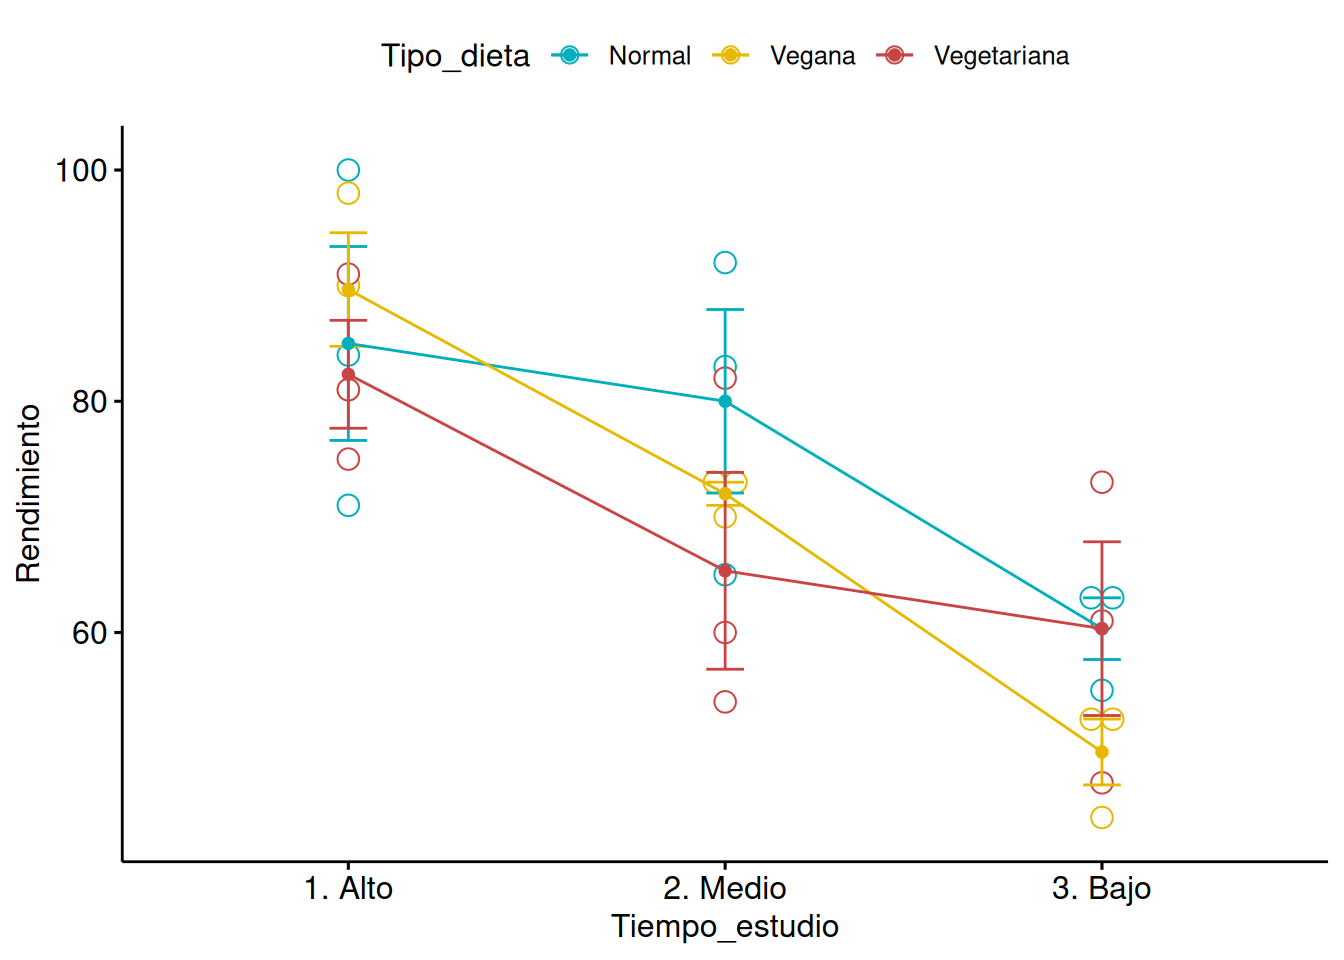
\includegraphics{anova_files/figure-pdf/datos_anova2_1-1.pdf}

}

\end{figure}

Realizamos el ANOVA de dos factores con interacción.

\begin{Shaded}
\begin{Highlighting}[]
\CommentTok{\# Realizar el ANOVA de dos factores con interacción}
\NormalTok{anova\_result }\OtherTok{\textless{}{-}} \FunctionTok{aov}\NormalTok{(Rendimiento }\SpecialCharTok{\textasciitilde{}}\NormalTok{ Tiempo\_estudio }\SpecialCharTok{*}\NormalTok{ Tipo\_dieta, }\AttributeTok{data =}\NormalTok{ datos)}

\CommentTok{\# Mostrar los resultados del ANOVA}
\FunctionTok{summary}\NormalTok{(anova\_result)}
\end{Highlighting}
\end{Shaded}

\begin{verbatim}
                          Df Sum Sq Mean Sq F value  Pr(>F)    
Tiempo_estudio             2   3765  1882.3  17.410 6.2e-05 ***
Tipo_dieta                 2    169    84.6   0.782   0.472    
Tiempo_estudio:Tipo_dieta  4    465   116.1   1.074   0.398    
Residuals                 18   1946   108.1                    
---
Signif. codes:  0 '***' 0.001 '**' 0.01 '*' 0.05 '.' 0.1 ' ' 1
\end{verbatim}

La interacción entre los dos factores no es estadísticamente
significativa a nivel \(\alpha=0.05\) y por lo tanto eliminamos dicha
fuente de variabilidad del modelo.

\begin{Shaded}
\begin{Highlighting}[]
\CommentTok{\# Realizar el ANOVA de dos factores sin interacción}
\NormalTok{anova\_result }\OtherTok{\textless{}{-}} \FunctionTok{aov}\NormalTok{(Rendimiento }\SpecialCharTok{\textasciitilde{}}\NormalTok{ Tiempo\_estudio }\SpecialCharTok{+}\NormalTok{ Tipo\_dieta, }\AttributeTok{data =}\NormalTok{ datos)}

\CommentTok{\# Mostrar los resultados del ANOVA}
\FunctionTok{summary}\NormalTok{(anova\_result)}
\end{Highlighting}
\end{Shaded}

\begin{verbatim}
               Df Sum Sq Mean Sq F value   Pr(>F)    
Tiempo_estudio  2   3765  1882.3  17.178 3.21e-05 ***
Tipo_dieta      2    169    84.6   0.772    0.474    
Residuals      22   2411   109.6                     
---
Signif. codes:  0 '***' 0.001 '**' 0.01 '*' 0.05 '.' 0.1 ' ' 1
\end{verbatim}

Podemos observar que el tipo de dieta no es un factor significativo en
el rendimiento académico. Por tanto, eliminamos dicho factor del modelo.

\begin{Shaded}
\begin{Highlighting}[]
\CommentTok{\# Realizar el ANOVA de un factor}
\NormalTok{anova\_result }\OtherTok{\textless{}{-}} \FunctionTok{aov}\NormalTok{(Rendimiento }\SpecialCharTok{\textasciitilde{}}\NormalTok{ Tiempo\_estudio , }\AttributeTok{data =}\NormalTok{ datos)}

\CommentTok{\# Mostrar los resultados del ANOVA}
\FunctionTok{summary}\NormalTok{(anova\_result)}
\end{Highlighting}
\end{Shaded}

\begin{verbatim}
               Df Sum Sq Mean Sq F value   Pr(>F)    
Tiempo_estudio  2   3765  1882.3   17.51 2.04e-05 ***
Residuals      24   2580   107.5                     
---
Signif. codes:  0 '***' 0.001 '**' 0.01 '*' 0.05 '.' 0.1 ' ' 1
\end{verbatim}

En cambio, el tiempo de estudio sí es un factor determinante en el
rendimiento académico. Su \(p-valor\) asociado es claramente inferior al
nivel de significancia \(0.05\).

Podemos visualizar el resultado:

\begin{Shaded}
\begin{Highlighting}[]
\CommentTok{\# Visualizar}
\FunctionTok{library}\NormalTok{(}\StringTok{"ggpubr"}\NormalTok{)}
\FunctionTok{ggline}\NormalTok{(datos, }\AttributeTok{x =} \StringTok{"Tiempo\_estudio"}\NormalTok{, }\AttributeTok{y =} \StringTok{"Rendimiento"}\NormalTok{,}
       \AttributeTok{add =} \FunctionTok{c}\NormalTok{(}\StringTok{"mean\_se"}\NormalTok{, }\StringTok{"dotplot"}\NormalTok{))}
\end{Highlighting}
\end{Shaded}

\begin{verbatim}
Bin width defaults to 1/30 of the range of the data. Pick better value with
`binwidth`.
\end{verbatim}

\begin{figure}[H]

{\centering 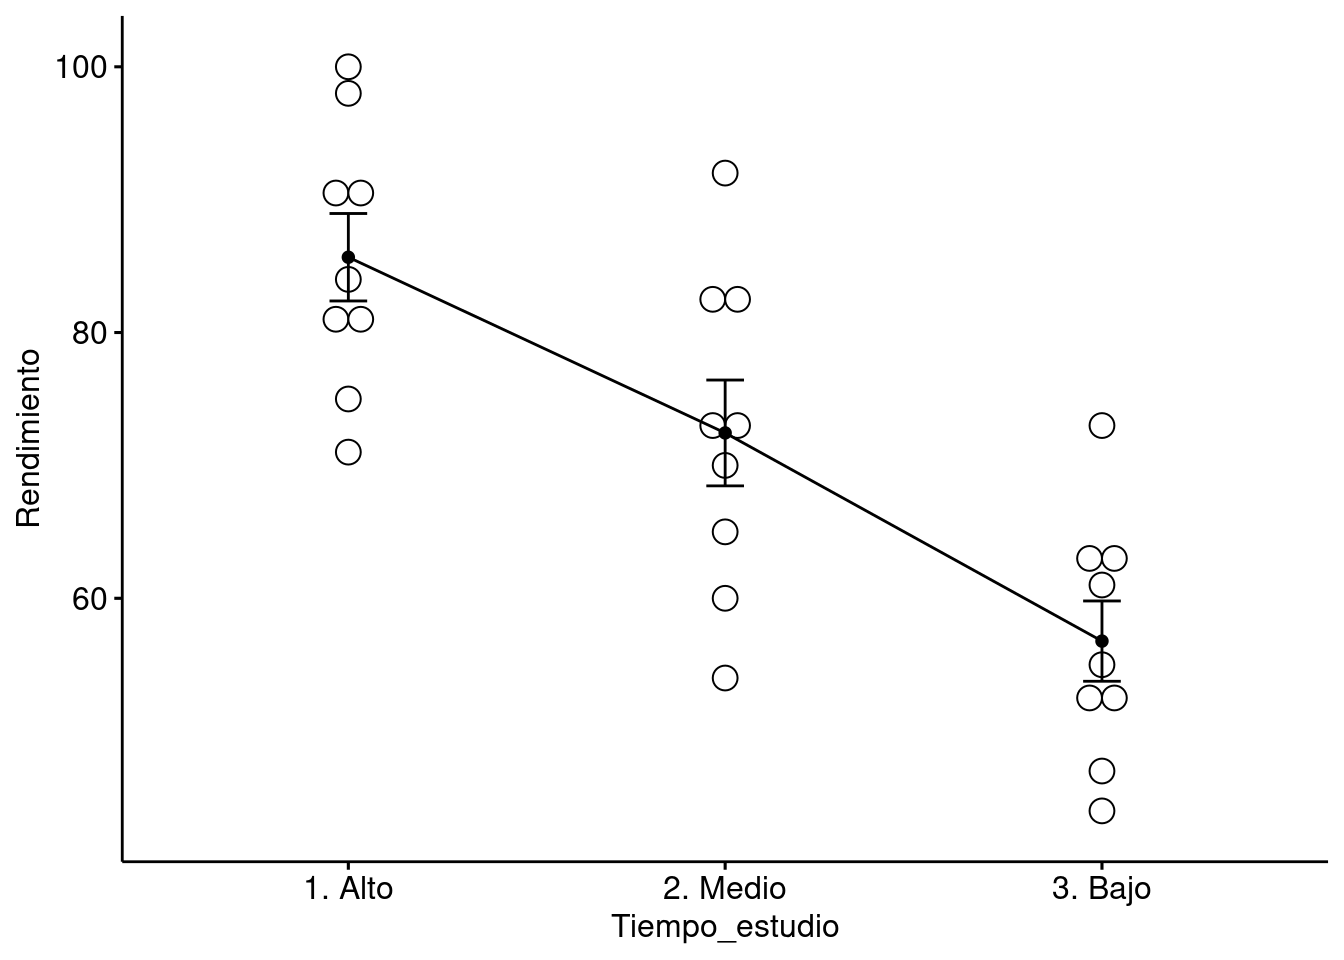
\includegraphics{anova_files/figure-pdf/anova_rend4-1.pdf}

}

\end{figure}

\end{tcolorbox}

\hypertarget{comparaciones-muxfaltiples}{%
\section{Comparaciones múltiples}\label{comparaciones-muxfaltiples}}

En el último ejemplo del apartado anterior hemos determinado que un
factor con \(3\) niveles era estadísticamente significativo. Es decir,
podemos rechazar la siguiente hipótesis nula:

\[H_O: \mu_1=\mu_2\ldots = \mu_k\] (con \(k\) igual al número de niveles
en el factor). Podemos plantearnos la pregunta siguiente: ¿En qué
niveles del factor se encuentran las principales diferencias? Es decir,
qué hipotesis (una o varias) de las siguientes son rechazadas:
\[H_O: \mu_1=\mu_2\] \[H_O: \mu_1=\mu_3\] \[\ldots\]
\[H_O: \mu_{k-1} = \mu_k\]

En un ejemplo con \(k=3\) niveles en el factor, es posible plantear
\(3\) contrastes de igualdad de medias, como los estudiados en capítulos
anteriores. En un ejemplo con \(k\) niveles en el factor, es posible
plantear \(k*(k-1)/2\) posibles contrastes de igualda de medias. Sin
embargo, si realizamos todos estos contrastes, aumenta la probabilidad
de cometer errores de tipo I (rechazar incorrectamente la hipótesis
nula). Este fenómeno se conoce como el \textbf{problema de las pruebas
múltiples}.

Como hemos venido viendo, cuando realizamos una sola prueba de hipótesis
(por ejemplo, una prueba \(t\) de Student o un ANOVA), generalmente
establecemos un nivel de significancia predeterminado, como
\(\alpha = 0.05\). Esto significa que estamos dispuestos a aceptar una
probabilidad de error de tipo I del \(5\%\), es decir, hay un \(5\%\) de
probabilidad de rechazar incorrectamente la hipótesis nula cuando es
verdadera.

Sin embargo, cuando realizamos múltiples pruebas de hipótesis, la
probabilidad acumulada de cometer al menos un error de tipo I aumenta
significativamente con cada prueba adicional. Por ejemplo, si realizamos
\(10\) pruebas de hipótesis independientes, cada una con un nivel de
significancia de \(\alpha = 0.05\), la probabilidad de cometer al menos
un error de tipo I aumenta a más del \(40\%\)
(\(1-(1-0.05)^{10}\approx 0.401\).

Existe una solución, \textbf{las comparaciones múltiples} necesarias
para controlar este aumento en el riesgo de error. Existen varios
métodos para controlar el problema de las pruebas múltiples, como los
ajustes de Bonferroni, Holm-Bonferroni, Holm, Hochberg,
Benjamini-Hochberg (FDR), entre otros. Estos métodos controlan la tasa
global de error de tipo I para todas las comparaciones realizadas,
manteniendo un nivel de significancia general específico.

\hypertarget{muxe9todo-de-bonferroni}{%
\subsection{Método de Bonferroni}\label{muxe9todo-de-bonferroni}}

El método de Bonferroni es una técnica comúnmente utilizada para
corregir el problema de las comparaciones múltiples y controlar el
riesgo de error de tipo I. Este método es relativamente simple y
conservador, lo que lo hace popular en muchas aplicaciones estadísticas.

La idea principal detrás del método de Bonferroni es ajustar el nivel de
significancia individual para cada prueba de hipótesis realizada. En
lugar de utilizar un nivel de significancia estándar (por ejemplo,
\(\alpha = 0.05\)), dividimos el nivel de significancia global deseado
(generalmente \(0.05\)) por el número total de pruebas realizadas
(\(m\)): \[
\alpha' = \frac{\alpha}{m}
\] Esta división produce un nivel de significancia más estricto
(\(\alpha'\)) para cada prueba individual, lo que ayuda a controlar el
riesgo global de error de tipo I.

Utilizamos el nivel de significancia individual ajustado para cada
prueba de hipótesis. Si el \(p-valor\) de una prueba es menor que el
nivel de significancia ajustado, rechazamos la hipótesis nula de la
prueba.

El método de Bonferroni es fácil de entender e implementar, y
proporciona un control conservador sobre el error de tipo I en
comparaciones múltiples. No obstante puede ser un método demasiado
conservador en situaciones donde se realizan muchas comparaciones, lo
que puede resultar en una pérdida de potencia estadística. Además, no
tiene en cuenta la correlación entre las pruebas realizadas.

\begin{tcolorbox}[enhanced jigsaw, arc=.35mm, breakable, coltitle=black, left=2mm, opacityback=0, bottomtitle=1mm, colbacktitle=quarto-callout-tip-color!10!white, title=\textcolor{quarto-callout-tip-color}{\faLightbulb}\hspace{0.5em}{Ejemplo. Comparaciones múltiples}, titlerule=0mm, colback=white, colframe=quarto-callout-tip-color-frame, bottomrule=.15mm, rightrule=.15mm, opacitybacktitle=0.6, toptitle=1mm, toprule=.15mm, leftrule=.75mm]

Continuamos con el ejemplo anterior anterior sobre la influencia del
tiempo de estudio en el rendimiento académico. Hemos visto que existe
una relación entre ambos factores. En otras palabras, hemos rechazado la
siguiente hipótesis nula:

\[
H_0: \mu_{Alto}=\mu_{Medio}=\mu_{Bajo}
\] Pero, ¿dónde se encuentran las diferencias relevantes?. Calculamos
las tres medias muestrales

\begin{Shaded}
\begin{Highlighting}[]
\FunctionTok{mean}\NormalTok{(datos[datos}\SpecialCharTok{$}\NormalTok{Tiempo\_estudio}\SpecialCharTok{==}\StringTok{"1. Alto"}\NormalTok{,]}\SpecialCharTok{$}\NormalTok{Rendimiento)}
\end{Highlighting}
\end{Shaded}

\begin{verbatim}
[1] 85.66667
\end{verbatim}

\begin{Shaded}
\begin{Highlighting}[]
\FunctionTok{mean}\NormalTok{(datos[datos}\SpecialCharTok{$}\NormalTok{Tiempo\_estudio}\SpecialCharTok{==}\StringTok{"2. Medio"}\NormalTok{,]}\SpecialCharTok{$}\NormalTok{Rendimiento)}
\end{Highlighting}
\end{Shaded}

\begin{verbatim}
[1] 72.44444
\end{verbatim}

\begin{Shaded}
\begin{Highlighting}[]
\FunctionTok{mean}\NormalTok{(datos[datos}\SpecialCharTok{$}\NormalTok{Tiempo\_estudio}\SpecialCharTok{==}\StringTok{"3. Bajo"}\NormalTok{,]}\SpecialCharTok{$}\NormalTok{Rendimiento)}
\end{Highlighting}
\end{Shaded}

\begin{verbatim}
[1] 56.77778
\end{verbatim}

Aplicamos el método de Bonferroni, y obtenemos:

\begin{Shaded}
\begin{Highlighting}[]
\FunctionTok{pairwise.t.test}\NormalTok{(datos}\SpecialCharTok{$}\NormalTok{Rendimiento, }\AttributeTok{g=}\NormalTok{datos}\SpecialCharTok{$}\NormalTok{Tiempo\_estudio,}\AttributeTok{p.adjust.method =} \StringTok{"bonferroni"}\NormalTok{)}
\end{Highlighting}
\end{Shaded}

\begin{verbatim}

    Pairwise comparisons using t tests with pooled SD 

data:  datos$Rendimiento and datos$Tiempo_estudio 

         1. Alto 2. Medio
2. Medio 0.037   -       
3. Bajo  1.3e-05 0.011   

P value adjustment method: bonferroni 
\end{verbatim}

Dado que todos los \(p-valores\) ajustados son menores que \(0.05\),
podemos rechazar las \(3\) hipótesis nulas. Es decir, rechazamos que el
rendimiento sea el mismo para los diferentes niveles de tiempos de
estudio.

Y en \texttt{R} podemos pintarlo como sigue (aquí empleamos otro método
de corrección diferente al de Bonferroni, revísalo)

\begin{Shaded}
\begin{Highlighting}[]
\NormalTok{comparaciones\_mult }\OtherTok{\textless{}{-}} \FunctionTok{TukeyHSD}\NormalTok{(anova\_result)}
\FunctionTok{plot}\NormalTok{(comparaciones\_mult)}
\end{Highlighting}
\end{Shaded}

\begin{figure}[H]

{\centering 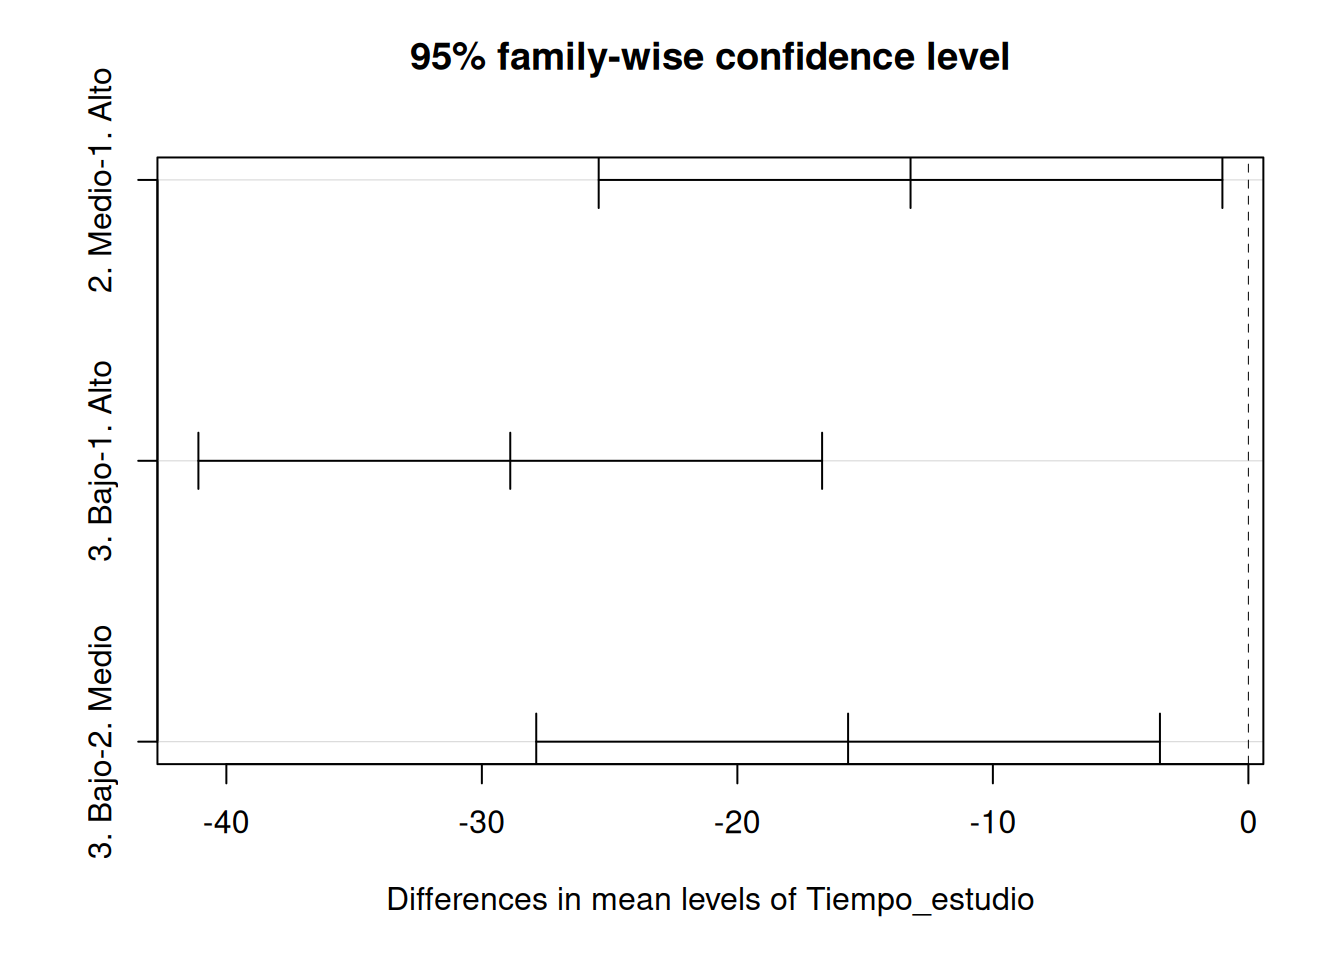
\includegraphics{anova_files/figure-pdf/plot_1-1.pdf}

}

\end{figure}

\end{tcolorbox}

\bookmarksetup{startatroot}

\hypertarget{sec-conclusiones}{%
\chapter{Conclusiones}\label{sec-conclusiones}}

A lo largo de cinco capítulos hemos presentado el material de la
asignatura de Inferencia Estadística del grado en Ciencia e Ingeniería
de Datos de la Universidad Rey Juan Carlos.

En este capítulo final, te proponemos reflexionar sobre las principales
lecciones aprendidas a lo largo del curso ``Inferencia Estadística'' y
destacaremos la importancia de las técnicas abordadas en la formación de
futuros profesionales en Ciencia e Ingeniería de Datos. Además,
alentaremos a los estudiantes a continuar explorando y ampliando sus
conocimientos en cursos posteriores.

Al finalizar este recorrido por los conceptos y técnicas de la
inferencia estadística, es evidente la importancia de esta disciplina en
el análisis y la interpretación de datos en el mundo moderno. A lo largo
de este libro, hemos explorado desde los fundamentos teóricos hasta las
aplicaciones prácticas, proporcionando a los estudiantes una base sólida
sobre la cual construir sus habilidades en ciencia de datos.

\hypertarget{resumen-de-los-aprendizajes}{%
\section{Resumen de los
aprendizajes}\label{resumen-de-los-aprendizajes}}

\begin{enumerate}
\def\labelenumi{\arabic{enumi}.}
\item
  \textbf{Comprensión de poblaciones y muestras}: Esperamos que hayas
  aprendido a distinguir entre población y muestra, comprendiendo la
  relevancia de los modelos probabilísticos y la importancia de asegurar
  un muestreo adecuado para obtener resultados representativos.
\item
  \textbf{Estimación de parámetros}: Juntos hemos abordado diversas
  técnicas de estimación puntual y por intervalos, permitiendo a los
  estudiantes realizar inferencias sobre parámetros de la población con
  un nivel de confianza adecuado.
\item
  \textbf{Contrastes de Hipótesis}: A lo largo del curso debes haber
  desarrollado la habilidad de plantear y resolver contrastes de
  hipótesis, una herramienta fundamental para la toma de decisiones
  informadas basadas en datos.
\item
  \textbf{Análisis de la Varianza (ANOVA)}: Se ha presentado, por
  primera vez en el Grado, el ANOVA como una técnica esencial para
  comparar múltiples grupos y entender las variaciones entre ellos,
  destacando su aplicación en diferentes contextos.
\item
  \textbf{Contrastes no paramétricos}: Para los casos donde las
  suposiciones paramétricas no se cumplen, se han introducido y aplicado
  métodos no paramétricos, ampliando el repertorio de herramientas
  disponibles para el trabajo futuro del científico e ingeniero de
  datos.
\end{enumerate}

\hypertarget{reflexiones-finales}{%
\section{Reflexiones finales}\label{reflexiones-finales}}

La inferencia estadística no solo es una herramienta académica, sino una
metodología aplicable en múltiples campos profesionales. Desde la
investigación científica hasta el análisis de mercados y la toma de
decisiones en negocios, la capacidad de interpretar datos y extraer
conclusiones válidas es una competencia esencial en la era de la
información.

Además, el enfoque en aplicaciones prácticas y el uso de R a lo largo de
este libro ha proporcionado a los estudiantes una experiencia directa
con herramientas de análisis de datos contemporáneas. Esta práctica no
solo refuerza los conceptos teóricos, sino que también prepara a los
estudiantes para enfrentar desafíos reales en su futura carrera
profesional.

\hypertarget{mirando-hacia-adelante}{%
\section{Mirando hacia adelante}\label{mirando-hacia-adelante}}

Con el conocimiento y las habilidades adquiridas, los estudiantes están
mejor equipados para explorar más a fondo el vasto campo de la ciencia
de datos. La estadística y la inferencia estadística seguirán
evolucionando con el avance de la tecnología y la disponibilidad de
datos. Por lo tanto, es crucial que los futuros profesionales mantengan
una mentalidad de aprendizaje continuo y estén abiertos a adoptar nuevas
metodologías y herramientas.

En conclusión, esperamos que este libro haya proporcionado una
comprensión profunda y práctica de la inferencia estadística, y que
inspire a los estudiantes a aplicar estos conocimientos con confianza y
creatividad en sus proyectos futuros. La capacidad de analizar datos de
manera crítica y tomar decisiones basadas en evidencias es una habilidad
poderosa y transformadora, que sin duda abrirá numerosas oportunidades
en el ámbito profesional.

Os recordamos que en próximos cursos os encontraréis con las asiganturas
de Regresión, Aprendizaje Automático I y Aprendizaje Automático II,
donde aplicaréis muchas de las técnicas y herramientas que hemos
aprendido juntos.

\textbf{¡Buena suerte!}

\bookmarksetup{startatroot}

\hypertarget{bibliografuxeda}{%
\chapter*{Bibliografía}\label{bibliografuxeda}}
\addcontentsline{toc}{chapter}{Bibliografía}

\markboth{Bibliografía}{Bibliografía}

\hypertarget{refs}{}
\begin{CSLReferences}{1}{0}
\leavevmode\vadjust pre{\hypertarget{ref-fox2018r}{}}%
Fox, John, and Sanford Weisberg. 2018. \emph{An r Companion to Applied
Regression}. Sage publications.

\leavevmode\vadjust pre{\hypertarget{ref-hao2019machine}{}}%
Hao, Jiangang, and Tin Kam Ho. 2019. {``Machine Learning Made Easy: A
Review of Scikit-Learn Package in Python Programming Language.''}
\emph{Journal of Educational and Behavioral Statistics} 44 (3): 348--61.

\leavevmode\vadjust pre{\hypertarget{ref-hastie2009elements}{}}%
Hastie, Trevor, Robert Tibshirani, Jerome H Friedman, and Jerome H
Friedman. 2009. \emph{The Elements of Statistical Learning: Data Mining,
Inference, and Prediction}. Vol. 2. Springer.

\leavevmode\vadjust pre{\hypertarget{ref-james2013introduction}{}}%
James, Gareth, Daniela Witten, Trevor Hastie, Robert Tibshirani, et al.
2013. \emph{An Introduction to Statistical Learning}. Vol. 112.
Springer.

\leavevmode\vadjust pre{\hypertarget{ref-kelleher2020fundamentals}{}}%
Kelleher, John D, Brian Mac Namee, and Aoife D'arcy. 2020.
\emph{Fundamentals of Machine Learning for Predictive Data Analytics:
Algorithms, Worked Examples, and Case Studies}. MIT press.

\leavevmode\vadjust pre{\hypertarget{ref-osmani2012learning}{}}%
Osmani, Addy. 2012. \emph{Learning JavaScript Design Patterns: A
JavaScript and jQuery Developer's Guide}. " O'Reilly Media, Inc.".

\leavevmode\vadjust pre{\hypertarget{ref-oualline2003practical}{}}%
Oualline, Steve. 2003. \emph{Practical c++ Programming}. " O'Reilly
Media, Inc.".

\leavevmode\vadjust pre{\hypertarget{ref-tukey1977exploratory}{}}%
Tukey, John W et al. 1977. \emph{Exploratory Data Analysis}. Vol. 2.
Reading, MA.

\leavevmode\vadjust pre{\hypertarget{ref-wirth2000crisp}{}}%
Wirth, Rüdiger, and Jochen Hipp. 2000. {``CRISP-DM: Towards a Standard
Process Model for Data Mining.''} In \emph{Proceedings of the 4th
International Conference on the Practical Applications of Knowledge
Discovery and Data Mining}, 1:29--39. Manchester.

\end{CSLReferences}

\hypertarget{refs}{}
\begin{CSLReferences}{1}{0}
\leavevmode\vadjust pre{\hypertarget{ref-fox2018r}{}}%
Fox, John, and Sanford Weisberg. 2018. \emph{An r Companion to Applied
Regression}. Sage publications.

\leavevmode\vadjust pre{\hypertarget{ref-hao2019machine}{}}%
Hao, Jiangang, and Tin Kam Ho. 2019. {``Machine Learning Made Easy: A
Review of Scikit-Learn Package in Python Programming Language.''}
\emph{Journal of Educational and Behavioral Statistics} 44 (3): 348--61.

\leavevmode\vadjust pre{\hypertarget{ref-hastie2009elements}{}}%
Hastie, Trevor, Robert Tibshirani, Jerome H Friedman, and Jerome H
Friedman. 2009. \emph{The Elements of Statistical Learning: Data Mining,
Inference, and Prediction}. Vol. 2. Springer.

\leavevmode\vadjust pre{\hypertarget{ref-james2013introduction}{}}%
James, Gareth, Daniela Witten, Trevor Hastie, Robert Tibshirani, et al.
2013. \emph{An Introduction to Statistical Learning}. Vol. 112.
Springer.

\leavevmode\vadjust pre{\hypertarget{ref-kelleher2020fundamentals}{}}%
Kelleher, John D, Brian Mac Namee, and Aoife D'arcy. 2020.
\emph{Fundamentals of Machine Learning for Predictive Data Analytics:
Algorithms, Worked Examples, and Case Studies}. MIT press.

\leavevmode\vadjust pre{\hypertarget{ref-osmani2012learning}{}}%
Osmani, Addy. 2012. \emph{Learning JavaScript Design Patterns: A
JavaScript and jQuery Developer's Guide}. " O'Reilly Media, Inc.".

\leavevmode\vadjust pre{\hypertarget{ref-oualline2003practical}{}}%
Oualline, Steve. 2003. \emph{Practical c++ Programming}. " O'Reilly
Media, Inc.".

\leavevmode\vadjust pre{\hypertarget{ref-tukey1977exploratory}{}}%
Tukey, John W et al. 1977. \emph{Exploratory Data Analysis}. Vol. 2.
Reading, MA.

\leavevmode\vadjust pre{\hypertarget{ref-wirth2000crisp}{}}%
Wirth, Rüdiger, and Jochen Hipp. 2000. {``CRISP-DM: Towards a Standard
Process Model for Data Mining.''} In \emph{Proceedings of the 4th
International Conference on the Practical Applications of Knowledge
Discovery and Data Mining}, 1:29--39. Manchester.

\end{CSLReferences}



\end{document}
